
\green{}

The Swarm project is set out to build permissionless storage and communication infrastructure for tomorrow's self-sovereign digital society. From a developer's perspective, Swarm is best seen as public infrastructure that powers real-time interactive web applications familiar from the \gloss{Web 2.0} era. It provides a low-level API to primitives that serve as building blocks of complex applications, as well as the basis for the tools and libraries for a Swarm-based \gloss{Web 3.0} development stack. The API and the tools are designed to allow access to the Swarm network from any traditional web browser, so that Swarm can immediately provide a private and decentralised alternative to today's \gloss{World Wide Web} (\gloss{WWW}).

\begin{figure}[htbp]
  \centering
    \includegraphics[width=0.8\textwidth]{fig/swarm-layered-design.pdf}
  \caption[Swarm's layered design \statusgreen]{Swarm's layered design}
\label{fig:Swarm-layered-design}
\end{figure}

This part details the design and architecture of the system. In accordance with the principles laid out in \ref{sec:design-principles}, we put an emphasis on modular design, and conceive of Swarm as having clearly separable layers, each dependent on the previous one (see Figure \ref{fig:Swarm-layered-design}):

\begin{itemize}[noitemsep]
\item (1) \emph{a peer-to-peer network protocol to serve as underlay transport,}
\item (2) \emph{an overlay network with protocols powering a distributed immutable storage of \glossplural{chunk} (fixed size data blocks),}
\item (3) \emph{a component providing high-level data access and defining APIs for base-layer features, and}
\item (4) \emph{an application layer defining standards, and outlining best practices for more elaborate use-cases.}
\end{itemize}

We regard (2) and (3) as the core of Swarm. Since the network layer relies on it, we will formulate also the requirements for (1), but we consider the detailed treatment of both (1) and (4) outside the scope of this book.


Central to the design, the architecture of Swarm's overlay network (layer 2 in Figure \ref{fig:Swarm-layered-design}) is discussed in Chapter \ref{sec:network} and complemented by Chapter \ref{sec:incentivisation}, describing the system of economic incentives which makes Swarm self-sustaining. In Chapter \ref{sec:high-level-functionality}, we introduce the algorithms and conventions that allow Swarm to map data concepts on to the chunk layer to enable the high-level functionalities for storage and communication, notably data structures such as filesystems and databases, \gloss{access control}, indexed \gloss{feeds} and direct messaging  which comprise layer 3 of Swarm.
In Chapter \ref{sec:persistence}, we present ways to prevent garbage collected chunks from disappearing from the network, including: \glossplural{erasure code}, \gloss{pinning} and insurance, and also provide ways to monitor, recover and re-upload them using missing chunk notifications and insurance challenges. 
Finally, in Chapter \ref{sec:ux}, we will look at functionality from a user-experience perspective.

\chapter{Network}\label{sec:network}

This chapter elaborates on how the Swarm overlay network is built on top of a \gloss{peer-to-peer} network protocol to form a topology that allows for the routing of messages between nodes (\ref{sec:topology-routing}). In \ref{sec:kademlia-storage}, we describe how such a network can serve as a scalable \gloss{distributed storage} solution for data chunks (\ref{sec:chunks}) and present the logic underpinning the protocols for retrieval/download and syncing/upload (\ref{sec:push-and-pull}).

\section{Topology and routing \statusgreen}\label{sec:topology-routing}

This section sets the scene (\ref{sec:underlay-transport}) for the \gloss{overlay network} (layer 2) of Swarm by making explicit the assumptions about the underlay network (layer 1). \ref{sec:overlay-addressing} introduces the \gloss{overlay address space} and explains how nodes are assigned an address. In  \ref{sec:kademlia-routing}, we present the \gloss{Kademlia} \gloss{overlay topology} (connectivity pattern) and explain how it solves routing between nodes. In \ref{sec:bootstrapping} we show how nodes running the Swarm client can discover each other, bootstrap and then maintain the overlay topology.

\subsection{Requirements for underlay network \statusyellow}\label{sec:underlay-transport} 

\yellow{}

Swarm is a network operated by its users. Each node in the network is supposed to run a client complying with the protocol specifications. On the lowest level, the nodes in the network connect using a peer-to-peer network protocol as their transport layer. This is called the \gloss{underlay network}. 
In its overall design, Swarm is agnostic of the particular underlay transport used as long as it satisfies the following requirements.

\begin{enumerate}[noitemsep]
    \item \emph{addressing} -- Nodes are identified by their \gloss{underlay address}.
    \item \emph{dialling} -- Nodes can initiate a direct connection to a peer by dialing them on their underlay address.
    \item \emph{listening} -- Nodes can listen to other peers dialing them and can accept incoming connections. Nodes that do not accept incoming connections are called \glossplural{light node}.
    \item \emph{live connection} -- A node connection establishes a channel of communication which is kept alive until explicit disconnection, so that the existence of a connection means the remote peer is online and accepting messages.
    \item \emph{channel security} -- 
    The channel provides identity verification and implements encrypted and authenticated transport resisting man-in-the-middle attacks.
    \item \emph{protocol multiplexing} -- 
    The underlay network service can accommodate several protocols running on the same connection. Peers communicate the protocols with the name and versions that they implement, and the underlay service identifies compatible protocols and starts up peer connections on each matched protocol. 
    \item \emph{delivery guarantees} -- 
    Protocol messages have \gloss{guaranteed delivery}, i.e. delivery failures due to network problems result in direct error response. 
    Order of delivery of messages within each protocol is guaranteed. 
    Ideally, the underlay protocol provides prioritisation. 
    If protocol multiplexing occurs on the same transport channel, this most likely implies framing to prevent long messages from blocking higher priority messages.
    \item \emph{serialisation} -- 
    The protocol message construction supports arbitrary data structure serialisation conventions.
    
\end{enumerate}

The \gloss{libp2p} library can provide all the needed functionality and is the designated underlay connectivity driver in the specification.%
%
\footnote{Swarm's initial Golang implementation uses Ethereum's \gloss{devp2p}/rlpx which satisfies the above criteria and uses TCP/IP with custom cryptography added for security. The underlay network address that devp2p uses is represented using the \gloss{enode URL scheme}. Devp2p dispatches protocol messages based on their message ID. It uses RLP serialisation which is extended with higher level data type representation conventions. In order to provide support for the Ethereum 1.x blockchain and for storing its state on Swarm, we may provide a thin devp2p node that proxies queries to the new libp2p-based Swarm client, or just uses its API. Otherwise we expect the devp2p networking support to be discontinued.}

\subsection{Overlay addressing\statusgreen}\label{sec:overlay-addressing} 
\green{}

While clients use the \gloss{underlay address} to establish connections to peers, each node running Swarm is additionally identified with an \gloss{overlay address}. It is this address that determines which peers a node will connect to and directs the way that messages are forwarded. The overlay address is assumed to be stable as it defines a node's identity across sessions and ultimately affects which content is most worth storing in the node's local storage.

The node's \gloss{overlay address} is derived from an Ethereum account by hashing the corresponding elliptic curve public key with the \gloss{BZZ network ID}, using the 256-bit Keccak algorithm. The decision to include the BZZ network ID is rooted in the fact that there can be multiple Swarm networks (e.g.\ test net, main net, or private Swarms), and serves to ensure that the same address cannot be used across different networks. Assuming any sample of base accounts are independently selected, the resulting overlay addresses are expected to have a uniform distribution in the address space of 256-bit integers. It is important to derive the address from a public key, as it allows the nodes to issue commitments associated with an overlay location using cryptographic signatures that are verifiable by 3rd parties. 

Using the long-lived communication channels of the \gloss{underlay network}, Swarm nodes form a network with \emph{quasi-permanent} peer connections. The resulting connectivity graph can then realise a particular topology defined over the address space. The \gloss{overlay topology} chosen is called \gloss{Kademlia}: It enables communication between any two arbitrary nodes in the Swarm network by providing a strategy to relay messages using only underlay peer connections. The protocol that describes how nodes share information with each other about themselves and other peers is called 'Hive'. How nodes use this protocol to bootstrap the \gloss{overlay topology} is discussed in \ref{sec:bootstrapping}. 
% The  theoretical basis for \gloss{Kademlia topology} is formalised rigorously in \ref{sec:kademlia-connectivity}. 

Crucially, the overlay address space encompasses the full range of 256-bit integers. Central to Swarm is the concept of \gloss{proximity order} (\gloss{PO}), which quantifies the relatedness of two addresses on a discrete scale.%
%
\footnote{Proximity order is the discrete logarithmic scale of proximity, which, in turn is the inverse of normalised XOR distance.% \cite{specs}. 
% See \ref{sec:proximity} for a formal definition.
}
%
Given two addresses, $x$ and $y$, $\mathit{PO}(x,y)$ counts the matching bits of their binary representation starting from the most significant bit up to the first one that differs. The highest proximity order is therefore 256, designating the maximum relatedness, i.e. where $x=y$.

\subsection{Kademlia routing \statusgreen}\label{sec:kademlia-routing}
\yellow{rework together with appendix}

\glossupper{Kademlia topology} can be used to route messages between nodes in a network using overlay addressing. It has excellent scalability as it allows for universal routing such that both (1) the number of hops and (2) the number of peer connections are always logarithmic to the size of the network. 

In what follows, we show the two common flavours of routing: \emph{iterative/zooming} and \emph{recursive/forwarding}. Swarm's design crucially relies on choosing the latter, forwarding flavour. However, this is unusual, and, as the iterative flavour predominates within much of the peer-to-peer literature and most other implementations are using iterative routing  (see \cite{maymounkov2002kademlia,baumgart2007s,lua2005survey}), we consider it useful to walk the reader through both approaches so their idiosyncrasies may be revealed.

\subsubsection{Iterative and forwarding Kademlia}

Let $R$ be an arbitrary binary relation over nodes in a network. Nodes that are in relation $R$ with a particular node $x$ are called \glossplural{peer} of $x$. Peers of $x$ can be indexed by their \gloss{proximity order} (\gloss{PO}) relative to $x$%
% (see \ref{sec:proximity})%
.
The equivalence classes of peers are called \glossplural{proximity order bin}, or just bins for short. Once arranged in bins, these groups of peers form the \gloss{Kademlia table} of the node $x$ (see Figure \ref{fig:kademlia-table}). 



\begin{figure}[htbp]
   \centering
    \includegraphics[width=.8\textwidth]{fig/kademlia-35.pdf}
   \caption[From overlay address space to Kademlia table \statusgreen]{From overlay address space to Kademlia table. \textbf{Top}: the overlay address space is represented with a binary tree, colored leaves are actual nodes. The path of the pivot node (+) is shown with thicker lines. \textbf{Centre}: peers of the pivot nodes are shown keyed by the bits of their xor distance measured from the pivot. Here, $0$s represent a matching bit with the pivot, and $1$s show a differing bit. The leaf nodes are ordered by their xor distance from the pivot (leftmost node). \textbf{Bottom}: the Kademlia table of the pivot: the subtrees branching off from the pivot path on the left are displayed as the rows of the table representing proximity order bins in increasing order.}
   \label{fig:kademlia-table}
\end{figure}

Node $x$ has a \gloss{saturated Kademlia table} if there is a $0\leq d_x\leq \mathit{maxPO}$ called the  \gloss{neighbourhood depth} such that (1) the node has at least one peer in each bin up to and excluding \gloss{proximity order} bin $d_x$ and (2) all nodes at least as near as $d_x$ (called the \gloss{nearest neighbours}) are peers of $x$. If each node in a network has a saturated Kademlia table, then we say that the network has \gloss{Kademlia topology}.

\begin{figure}[htbp]
   \centering
    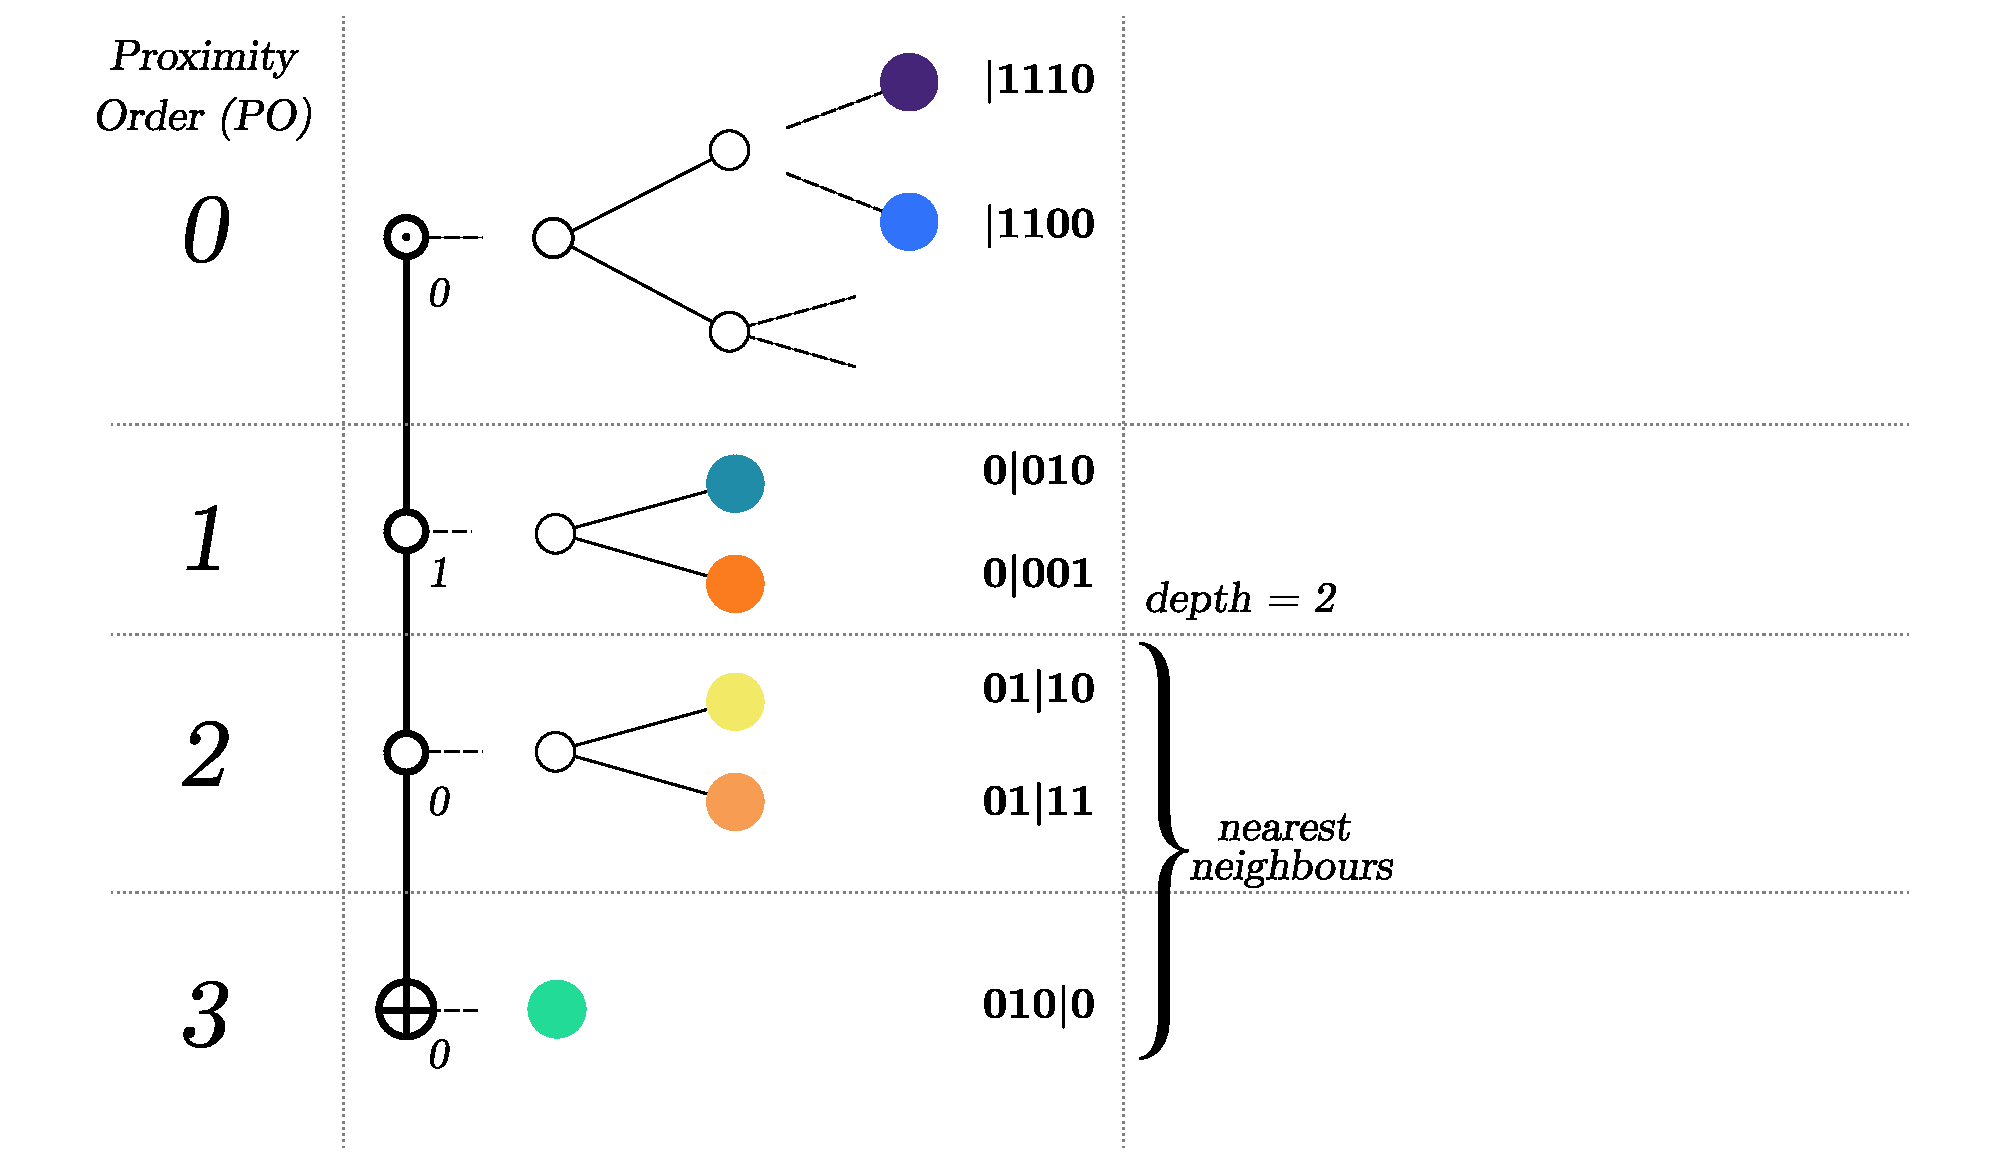
\includegraphics[width=\textwidth]{fig/kademlia-3.pdf}
   \caption[Nearest neighbours \statusgreen]{Nearest neighbours in a 4 bit network with $d = 2$ }
   \label{fig:bin-density}
\end{figure}

Let $R$ be the "is known to" relation:  $y$ "is known to" $x$ if $x$ has both overlay and underlay addressing information for $y$. 
In iterative Kademlia routing, the \gloss{requestor node} iteratively extends the graph of peers that are known to it. Using their \gloss{underlay address}, the requestor node will contact the peers that they know are nearest the destination address for peers that are further away (commonly using UDP). On each successive iteration, the peers become at least one order closer to the destination (see Figure \ref{fig:iterative-forwarding-kademlia}). Because of the Kademlia criteria, the requestor will eventually discover the destination node's underlay address and can then establish direct communication with it. This iterative strategy%
%
\footnote{The iterative protocol is equivalent to the original Kademlia routing that is described in \cite{maymounkov2002kademlia}.
}
%
critically depends on the nodes' ability to find peers that are currently online. In order to find such a peer, a node needs to collect several candidates for each bin. The best predictor of availability is the recency of the peer's last response, so peers in a bin should be prioritised according to this ordering.

\begin{figure}[htbp]
   \centering
   \vspace{-2cm} 
   \includegraphics[width=.8\textwidth]{fig/iterative-kademlia.pdf}\\\vspace{-1.3cm}
   \includegraphics[width=.8\textwidth]{fig/forwarding-kademlia-3.pdf}
   \caption[Iterative and Forwarding Kademlia routing \statusgreen]{Iterative and Forwarding Kademlia routing: A requestor node shown with a cross in the circle at address $...0000...$ wants to route to a destination address $...1111...$ to which the closest peer online is the blue circle at $...1110...$ These initial ellipses represent the prefix shared by requestor and destination addresses which is $n$ bits long. \textbf{Top:} In the iterative flavour, the requestor contacts the peers (Step 1, dotted black arrows) that they know are nearest the destination address. Peers that are online (yellow) respond with information about nodes that are even closer (green arrow, Step 2) so the requestor can now repeat the query using these closer peers (green, Step 3). On each successive iteration, the peers (yellow, green and blue) are at least one PO closer to the destination until eventually the requestor is in direct contact with the node that is nearest to the destination address. \textbf{Bottom:} In the forwarding flavour, the requestor forwards a message to the connected peer they know that is nearest to the destination (yellow). The recipient peer does the same. Applying this strategy recursively relays the message via a chain of peers (yellow, green, blue) each at least one PO closer to the destination.}
   \label{fig:iterative-forwarding-kademlia}
\end{figure}


Swarm uses an alternative flavour of Kademlia routing, which is first described in \cite{heep2010r} and then expanded on and worked out in \cite{tronetal2019-network}. Here, a recursive method is employed, whereby the successive steps of the iteration are "outsourced" to a \gloss{downstream peer}.
Each node recursively passes a message to a direct peer at least one \gloss{proximity order} closer to the destination. Thus, \gloss{routing} using this approach simply means relaying messages via a chain of peers which are ever closer to the destination, as shown in Figure \ref{fig:iterative-forwarding-kademlia}.


In this way, Swarm's underlay transport offers quasi-stable peer connections over TCP with communication channels that are kept alive. These open connections can then be used as $R$ to define another notion of a \gloss{peer}. The two criteria of healthy \gloss{Kademlia connectivity} in Swarm translate as: For each node $x$, there exists a \gloss{neighbourhood depth} $d_x$ such that (1) node $x$ has an open connection with at least one node for each \gloss{proximity order bin} up to but excluding $d_x$, and (2) is connected to all the online nodes that are at least as near as $d_x$. If each node in the network has a saturated Kademlia table of peers, then the network is said to have \gloss{Kademlia topology}. Since connected peers are guaranteed to be online, the recursive step consists solely of forwarding the message to a connected peer strictly closer to the destination. We can call this alternative \gloss{forwarding Kademlia}.


In a \gloss{forwarding Kademlia} network, a message is said to be \emph{routable} if there exists a path from sender to destination through which the message can be relayed. In a mature subnetwork with \gloss{Kademlia topology} every message is routable. 

If all peer connections are stably online, a \gloss{thin Kademlia table}, i.e.\ a single \gloss{peer} for each bin up to $d$, is sufficient to guarantee routing between nodes. In reality, however, networks are subject to \gloss{churn}, i.e.\ nodes are expected to go offline regularly. In order to ensure \gloss{routability} in the face of churn, the network needs to maintain \gloss{Kademlia topology}. This means that each individual node needs to have a \gloss{saturated Kademlia table} at all times. By keeping several connected peers in each \gloss{proximity order bin}, a node can ensure that node dropouts do not damage the saturation of their Kademlia table. Given a model of node dropouts, we can calculate the minimum number of peers needed per bin to guarantee that nodes are saturated with a probability that is arbitrarily close to 1. The more peers a node keeps in a particular proximity order bin, the more likely that the message destination address and the peer will have a longer matching prefix. As a consequence of forwarding the message to that peer, the \gloss{proximity order} increases more quickly, and the message ends up closer to the destination than it would with less peers in each bin (see also Figure \ref{fig:bindensity}).



With \gloss{Kademlia} saturation guaranteed, a node will always be able to forward a message and ensure \gloss{routability}. If nodes comply with the forwarding principles (and that is ensured by aligned incentives), the only case when relaying could possibly break down is when a node drops out of the network after having received a message but before it managed to forward it.%
%
\footnote{Healthy nodes could commit to being able to forward within a (very short) constant time; let's call this the \gloss{forwarding lag}. In the case that a \gloss{downstream peer} disconnects before this forwarding lag passes, then the \gloss{upstream peer} can re-forward the message to an alternative peer, thereby keeping the message passing unbroken. See \ref{sec:retrieval} for more detail.
} 

An important advantage of forwarding Kademlia is that this method of routing requires a lot less bandwidth than the iterative algorithm. In the iterative version, known peers are not guaranteed to be online, so finding one that is available adds an additional level of unpredictability.

\subsubsection{Sender anonymity}
\glossupper{sender anonymity} is a crucial feature of Swarm. It is important that peers further down in the request cascade can never know who the originator of the request was, because requests are relayed from peer-to-peer. 

The above rigid formulation of Kademlia routing would suggest that if a node receives a message from a peer and that message and peer have a proximity order of $0$, then the recipient would be able to conclude that the peer it received the message from must be the sender. If we allow \gloss{light node} Swarm clients, i.e. clients that due to resource constraints do not keep a full Kademlia saturation but instead have just a local neighbourhood, then even a message from a peer in bin $0$ remains of ambiguous origin. 

\subsubsection{Bin density and multi-order hops} \label{sec:bindensity}

As a consequence of logarithmic distance and uniform node distribution, the population of peers exponentially increases as we move further away from a particular node.
This means that unless the number of required connections in a bin doubles as bins increase in distance from the node, shallower bins will always allow more choice of nodes for potential connection. In particular, nodes have a chance to increase the number of connections per bin in such a way that peer addresses maximise density (i.e., in proximity order bin $b$, the subsequent bits of peer addresses form a \gloss{balanced binary tree}). Such an arrangement is optimal in the sense that for a bin depth of $d$, nodes are able to relay all messages so that in one hop the proximity order of the destination address will increase by $d$ (see Figure \ref{fig:bindensity}). 


\begin{figure}[htbp]
   \centering
   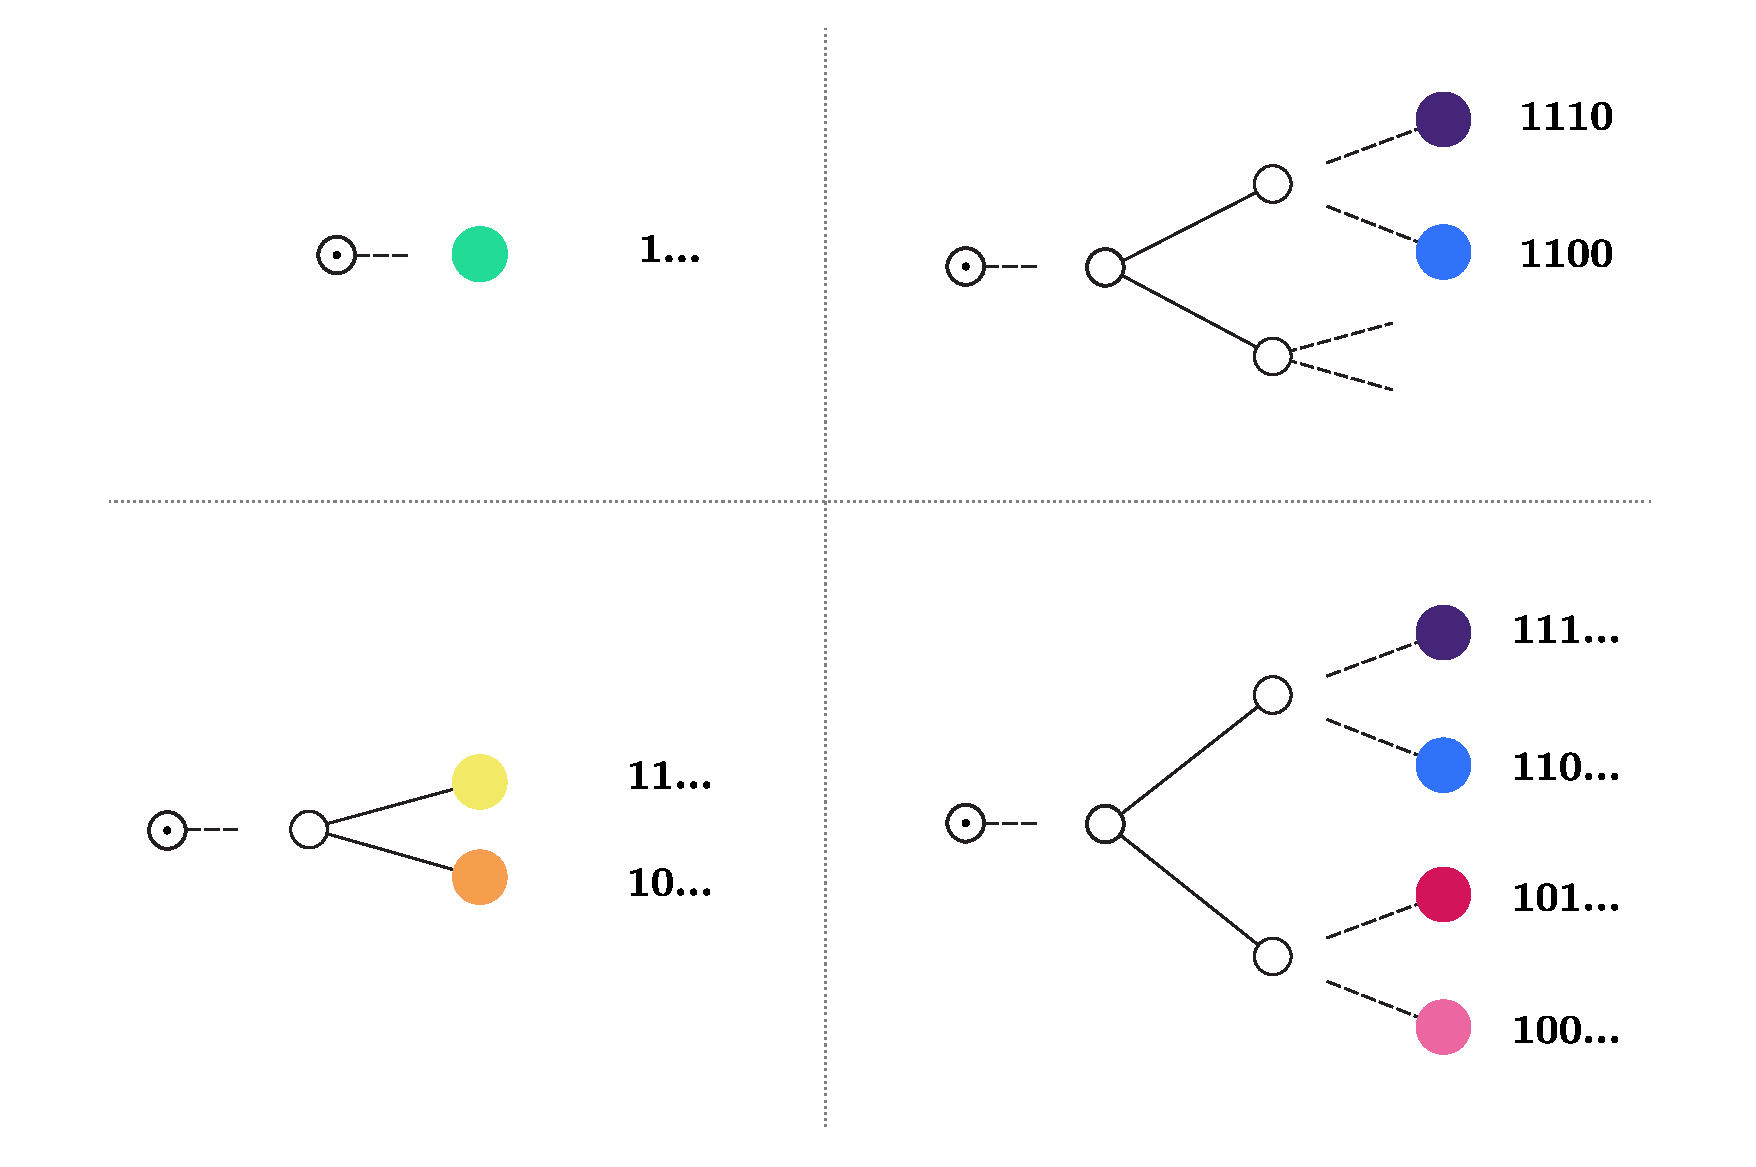
\includegraphics[width=\textwidth]{fig/bindensity.pdf}
   \caption[Bin density \statusgreen]{Bin density:  types of saturation for PO bin $0$ for a node with overlay address starting with bit $0$. \textbf{Top left}: A "thin" bin with a single peer is not resilient to churn and only increases PO by $1$ in one hop. \textbf{Top right:} At least two peers are needed to maintain Kademlia topology in case of churn; two peers when not balanced cannot guarantee multi-order hops. \textbf{Bottom left:} Two peers balanced guarantees an increase of 2 POs in one hop. \textbf{Bottom right:} Four peers, when balanced, can guarantee an increase of $3$ POs in one hop.}
   \label{fig:bindensity}
\end{figure}

\subsubsection{Factoring in underlay proximity}
It is expected that as Swarm clients continue to evolve and develop, nodes may factor in throughput when they select peers for connection. All things being equal, nodes physically closer to each other tend to have higher throughput, and therefore will be preferred in the long run. This is how forwarding Kademlia is implicitly aware of the underlay topology \cite{heep2010r}. 


\subsection{Bootstrapping and maintaining Kademlia topology \statusgreen}\label{sec:bootstrapping}
 
\orange{rework based on new hive protocol}
 
This section discusses how a stable Kademlia topology can emerge. In particular, it outlines the exact bootstrapping protocol that each node must follow to reach and maintain a saturated Kademlia connectivity. Nodes joining a \gloss{decentralised network} are supposed to be initially naive, potentially initiating connection via only a single known peer with no prior knowledge. For this reason, the bootstrapping process needs to include an initial step that helps naive nodes to begin exchanging information about each other. This discovery process is called the \gloss{hive protocol}.

\subsubsection{Bootnodes}

Swarm has no distinct node type or operation mode for bootnodes. This means that naive nodes should be able to connect to any node on the  network and bootstrap their desired connectivity. In order not to overburden any single node, electing one particular node as an initial connection should be avoided, and the role of being a bootnode for the newly connecting naive nodes should ideally be distributed among participant nodes. This is achieved either with an invite system, or a centralised bootnode service running a public gateway that responds to an API call with the bzz address of a randomly chosen node among online peers. 

Once connected to a node in the network, the hive protocol kicks in and the naive node begins to learn about the bzz addresses of other nodes, and thus it can start bootstrapping its connectivity.

\subsubsection{Building up connections}

Initially, each node begins with zero as their \gloss{saturation depth}. Nodes keep advertising their saturation depth to their connected peers as it changes. When a node $A$ receives an attempt to establish a new connection from a node $B$, she notifies each of her other peers about $B$ connecting to her only in the case that each peer's proximity order relative to the connecting node $A$ is not lower than that peer's advertised saturation depth. The notification is always sent to a peer that shares a proximity order bin with the new connection. Formally, when $y$ connects to $x$, $x$ notifies a subset of its connected peers. A peer $p$ belongs to this subset if $\mathit{PO}(x, p) = \mathit{PO}(x, y)$ or $d_p\leq \mathit{PO}(y, p)$. The notification takes the form of a protocol message and includes the full \gloss{overlay address} and \gloss{underlay address} information.%
%
\footnote{Light nodes that do not wish to relay messages and do not aspire to build up a healthy Kademlia are not included, see Section \ref{sec:light}. }

    

% \begin{figure}[htbp]
%   \centering
%   \caption[Hive protocol: bootstrapping and maintaining Kademlia topology \statusred]{Hive protocol: bootstrapping and maintaining Kademlia topology}
%   \label{fig:bootstrapping-kademlia}
% \end{figure}

\subsubsection{Mature connectivity}

After a sufficient number of nodes are connected, a bin becomes saturated and the node's neighbourhood depth can begin to increase. Nodes keep their peers up to date by advertising their current depth if it changes. As their depth increases, nodes will get notified of fewer and fewer peers. Once the node finds all their nearest neighbours and has saturated all the bins, no new peers are to be expected. For this reason, a node can conclude a saturated Kademlia state if it receives no new peers for some time.%
%
\footnote{Note that the node does not need to know the total number of nodes in the network. In fact, some time after the node stops receiving new peer addresses, the node can effectively estimate the size of the network: the depth of network is $\log_2(n+1)+ d$ where $n$ is the number of remote peers in the nearest neighbourhood and $d$ is the depth of that neighbourhood. It then follows that the total number of nodes in the network can be estimated simply by taking this to the power of 2.}
%
Instead of having a hard deadline and a binary state of saturation, we can quantify the certainty of saturation by considering the time elapsed since the arrival of the most recent new peer. Assuming stable connections, eventually each node online will get to know its nearest neighbours and connect to them while keeping each bin up to $d$ non-empty. Therefore each node will converge on the saturated state. To maintain a robust Kademlia topology in the face of changing peer connections, it is crucial to include multiple peers within each proximity order bin. This prevents the node from regressing to a lower saturation state, even when there are no new nodes joining the network. 

\section{Swarm storage\statusgreen}\label{sec:kademlia-storage}

In this section, in \ref{sec:disc}, we first show how a network with quasi-permanent connections in a Kademlia topology can support a \gloss{load balancing}, \gloss{distributed storage} of fixed-sized data blobs. In \ref{sec:chunks}, we detail the generic requirements on chunks and introduce actual chunk types. Finally, in \ref{sec:redundancy-by-local-replication}, we turn to \gloss{redundancy} by neighbourhood replication as a first line of defense against node churn.

\subsection{Distributed immutable store for chunks\statusgreen}\label{sec:disc}
 
In this section, we discuss how networks using Kademlia overlay routing are a suitable basis on which to implement a serverless storage solution using \glossplural{distributed hash table} (\glossplural{DHT}). Then we introduce the \gloss{DISC}%
%
\footnote{DISC is \gloss{distributed immutable store for chunks}. In earlier work, we have referred to this component as the 'distributed preimage archive' (DPA), however, this phrase became misleading since we now also allow chunks that are not the preimage of their address.}
% 
model, Swarm's narrower interpretation of a DHT for storage. This model 
imposes some requirements on chunks and necessitates 'upload' protocols. 

As is customary in Swarm, we provide a few resolutions of this acronym, which summarise the most important features:


\begin{itemize}
\item \emph{decentralised infrastructure for storage and communication}, 
\item \emph{distributed immutable store for chunks}, 
\item \emph{data integrity by signature or content address},
% \item \emph{downloadable incentivised secure communications}
\item \emph{driven by incentives with smart contracts}. 

\end{itemize}
 
\subsubsection{From DHT to DISC}
Swarm's \gloss{DISC} shares many similarities with widely known \glossplural{distributed hash table}. The most important difference is that Swarm does not keep track of \emph{where} files are to be found, instead it actually \emph{stores pieces of the file itself} directly with the closest node(s). 
In what follows, we review DHTs, as well as dive into the similarities and differences with DISC in more detail. 
 
\glossupperplural{distributed hash table} use an overlay network to implement a key--value container distributed over the nodes (see Figure \ref{fig:DHT}). The basic idea is that the keyspace is mapped onto the overlay address space, and the value for a key in the container is to be found with nodes whose addresses are in the proximity of the key. In the simplest case, let us say that this is the single closest node to the key that stores the value. In a network with Kademlia connectivity, any node can route to a node whose address is closest to the key, therefore a \emph{lookup} (i.e.\ looking up the value belonging to a key) is reduced simply to routing a request. 

\begin{figure}[htbp]
   \centering
   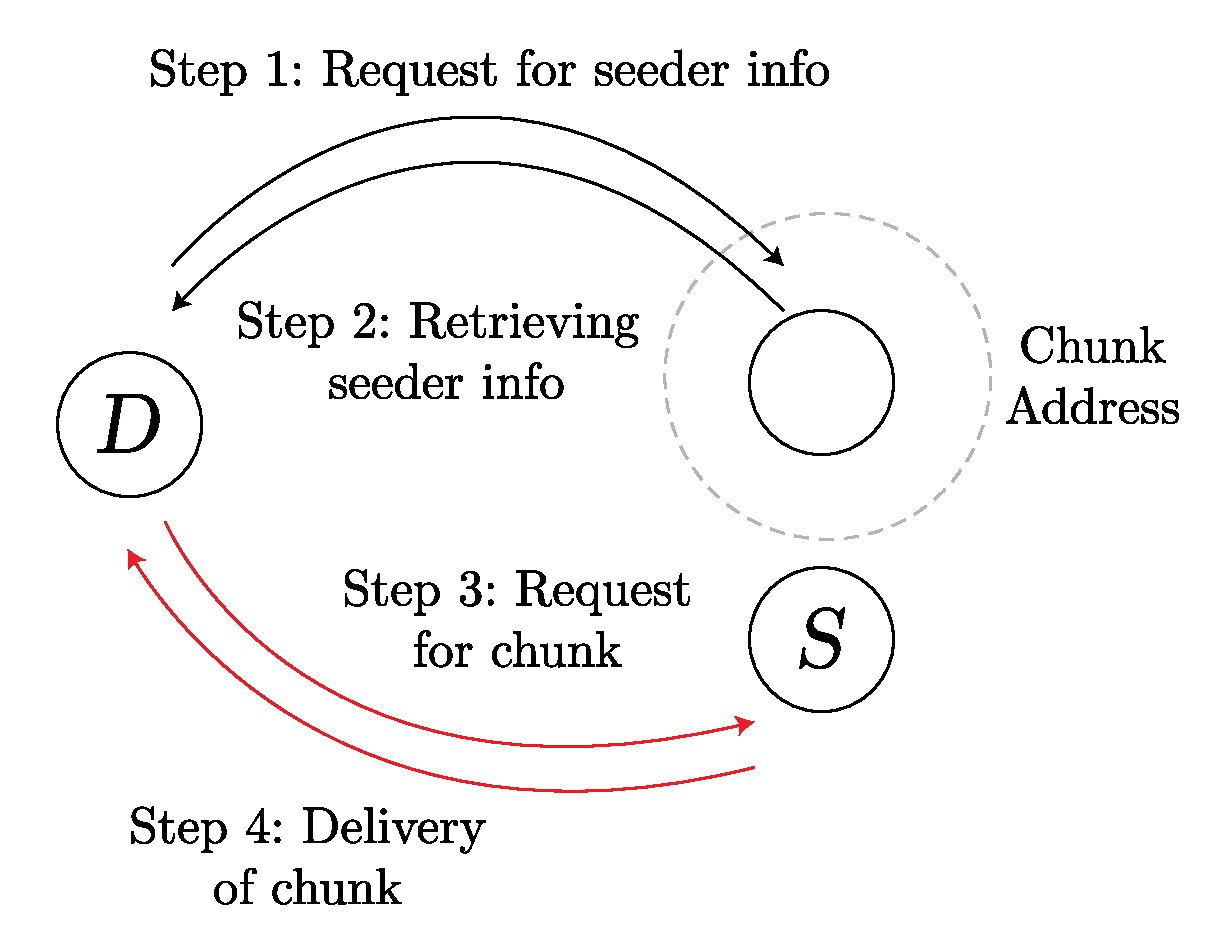
\includegraphics[width=0.7\textwidth]{fig/dht.pdf}
   \caption[Distributed hash tables (DHTs) \statusgreen]{Distributed hash tables (DHTs) used for storage:  node $D$ (downloader) uses Kademlia routing in Step $1$ to query nodes in the neighbourhood of the chunk address to retrieve seeder info in Step $2$. The seeder info is used to contact node $S$ (seeder) directly to request the chunk and deliver it in Steps $3$ and $4$.}
   \label{fig:DHT}
\end{figure}

DHTs used for \gloss{distributed storage} typically associate content identifiers (as keys/addresses) with a changing list of seeders (as values) that can serve that content \cite{ipfs2014, crosby2007analysis}. However, the same structure can be used directly: in Swarm, it is not information about the location of content that is stored at the node closest to the address, but the content itself (see Figure \ref{fig:disc}). 


\begin{figure}[htbp]
   \centering
   \includegraphics[width=0.7\textwidth]{fig/disc.pdf}
   \caption[Swarm DISC: Distributed Immutable Store for Chunks \statusgreen]{Swarm DISC:  Distributed Immutable Store for Chunks. In Step $1$, downloader node $D$ uses forwarding Kademlia routing to request the chunk from a storer node $S$ in the neighbourhood of the chunk address. In Step $2$ the chunk is delivered along the same route using forwarding step just backwards.}
   \label{fig:disc}
\end{figure}

\subsubsection{Constraints}
The \gloss{DISC} storage model is opinionated about which nodes store what content and this implies the following restrictions: 

\begin{enumerate}
    \item \emph{fixed-size chunks} -- Load balancing of content is required among nodes and is realised by splitting content into equal-sized units called \glossplural{chunk} (see \ref{sec:chunks}).
    \item \emph{syncing} -- There must be a process whereby chunks get to where they are supposed to be stored, no matter which node uploads them (see \ref{sec:push-syncing}).
    \item \emph{plausible deniability} -- Since nodes do not have a say in what they store, measures should be employed that serve as the basis of legal protection for node operators. They need to be able to plausibly deny knowing (or even being able to know) anything about the chunks' contents (see \ref{sec:chunk-encryption}).
    \item \emph{garbage collection} -- Since nodes commit to store any data close to them, there needs to be a strategy to select which chunks are kept and which are discarded in the presence of storage space constraints. 
\end{enumerate}

\subsubsection{Chunks}\label{sec:chunks}

\glossupperplural{chunk} are the basic storage units used in Swarm's network layer. They are an association of an address with content. Since retrieval in Swarm (\ref{sec:retrieval}) assumes that chunks are stored with nodes close to their address, fair and equal \gloss{load balancing} requires that the addresses of chunks should also be uniformly distributed in the address space, and have their content limited and roughly uniform in size.  

When chunks are retrieved, the downloader must be able to verify the correctness of the content given the address. Such integrity translates to guaranteeing uniqueness of content associated with an address. In order to protect against frivolous network traffic, a third party of \glossplural{forwarding node} should be able to verify the integrity of chunks using only local information available to the node.

The deterministic and collision-free nature of addressing implies that chunks are unique as a key--value association: If there exists a chunk with an address, then no other valid chunk can have the same address; this assumption is crucial as it makes the chunk store \gloss{immutable}, i.e.\ there is no replace/update operation on chunks. Immutability is beneficial in the context of relaying chunks as nodes can negotiate information about the possession of chunks simply by checking their addresses. This plays an important role in the stream protocol (see \ref{sec:pull-syncing}) and justifies the DISC resolution as a \emph{distributed immutable store for chunks}.

To sum up, chunk addressing needs to fulfill the following requirements:

\begin{enumerate}
    \item \emph{deterministic} -- To enable local validation.
    \item \emph{collision-free} -- To provide integrity guarantee.
    \item \emph{uniformly distributed} -- To deliver load balancing.
\end{enumerate}

In the current version of Swarm, we support two types of chunks: \glossplural{content addressed chunk} and \glossplural{single owner chunk}. 

\subsection{Content addressed  chunks\statusgreen}\label{sec:content-addressed-chunks}

A \gloss{content addressed chunk} is not assumed to be a meaningful storage unit, i.e. they can be just blobs of arbitrary data resulting from splitting a larger data blob, a file. The methods by which files are disassembled into chunks when uploading and then reassembled from chunks when downloading are detailed in \ref{sec:datastructures}. The data size of a content addressed Swarm chunk is limited to 4 kilobytes. One of the desirable consequences of using this small chunk size is that concurrent retrieval is available even for relatively small files, reducing the latency of downloads. 

\begin{figure}[htbp]
   \centering
   
\includegraphics[width=\textwidth]{fig/content-addressed-chunk-3.pdf}
   \caption[Content addressed chunk\statusgreen]{Content addressed chunk. An at most 4KB payload with a 64-bit little-endian encoded span prepended to it constitutes the chunk content. The BMT hash of the payload concatenated with the span then yields the content address.}
   \label{fig:content-addressed-chunk}
\end{figure}

\subsubsection{Binary Merkle tree hash}

The canonical content addressed chunk in Swarm is called a \gloss{binary Merkle tree chunk} (\gloss{BMT chunk}).
The address of BMT chunks is calculated using the \gloss{binary Merkle tree hash} algorithm (\gloss{BMT hash}). The base hash used in \gloss{BMT} is Keccak256, properties of which such as uniformity, irreversibility, and collision resistance all carry over to the \gloss{BMT hash} algorithm. As a result of uniformity, a random set of chunked content will generate addresses evenly spread in the address space, i.e.\ imposing storage requirements balanced among nodes.


\begin{figure}[htbp]
   \centering
   \resizebox{1\textwidth}{!}{
   \input{fig/bmthash.tex}}
   \caption[BMT: Binary Merkle Tree hash used as chunk hash in Swarm \statusgreen]{BMT (Binary Merkle Tree) chunk hash in Swarm: the 1337 bytes of chunk data is segmented into 32-byte segments. Zero padding is used to fill up the rest up to 4 kilobytes. Pairs of segments are hashed together using Keccak256 to build up the binary tree. On level 8, the binary Merkle root is prepended with the 8-byte span and hashed to yield the BMT chunk hash.}
   \label{fig:BMT}
\end{figure}

The BMT chunk address is the hash of the 8-byte span and the root hash of a \gloss{binary Merkle tree} (\gloss{BMT}) built on the 32-byte segments of the underlying data (see Figure \ref{fig:BMT}). If the chunk content is less than 4k, the hash is calculated as if the chunk was padded with all zeros up to 4096 bytes.

This structure allows for compact \gloss{inclusion proofs} with a 32-byte resolution. An inclusion proof is a proof that one string is a substring of another string, for instance, that a string is included in a chunk. Inclusion proofs are defined on a data segment of a particular index, see Figure \ref{fig:chunk-inclusion}. Such Merkle proofs are also used as proof of custody when storer nodes provide evidence that they possess a chunk (see \ref{sec:redistribution}). Together with the Swarm file hash (see \ref{sec:files}), they allow for logarithmic inclusion proofs for files, i.e.,\ proof that a string is found to be part of a file.


\begin{figure}[htbp]
\centering
\includegraphics[width=\textwidth]{fig/inclusion-proof.pdf}
\caption[Compact segment inclusion proofs for chunks \statusgreen]{Compact segment inclusion proofs for chunks. Assume we need proof for segment 26 of a chunk (yellow). The orange hashes of the BMT are the sister nodes on the path from the data segment up to the root and constitute what needs to be part of a proof. When these are provided together with the root hash and the segment index, the proof can be verified. The side on which proof item $i$ needs to be applied depends on the $i$-th bit (starting from least significant) of the binary representation of the index. Finally, the span is prepended and the resulting hash should match the chunk root hash.}
\label{fig:chunk-inclusion}
\end{figure}


\subsection{Single owner chunks\statusgreen}\label{sec:single-owner-chunks}

With \glossplural{single owner chunk}, a user can assign arbitrary data to an address and attest chunk integrity with their digital signature. The address is calculated as the hash of an \gloss{identifier} and an \gloss{owner}. The chunk content is presented in a  structure composed of the identifier, the \gloss{payload}, and a signature attesting to the association of identifier and payload (see Figure \ref{fig:single-owner-chunks}).

\begin{itemize}
    \item \emph{content}: 
\begin{itemize}
    \item \emph{identifier} -- 32 bytes arbitrary identifier, 
    \item \emph{signature} -- 65 bytes $\langle r,s,v \rangle$ representation of an EC signature (32+32+1 bytes),
    \item \emph{span} -- an 8-byte little-endian binary of uint64 chunk span,
    \item \emph{payload} -- maximum 4096 bytes of regular chunk data.
\end{itemize}
    \item \emph{address} -- Keccak256 hash of identifier + owner account.
\end{itemize}

\begin{figure}[htbp]
   \centering
   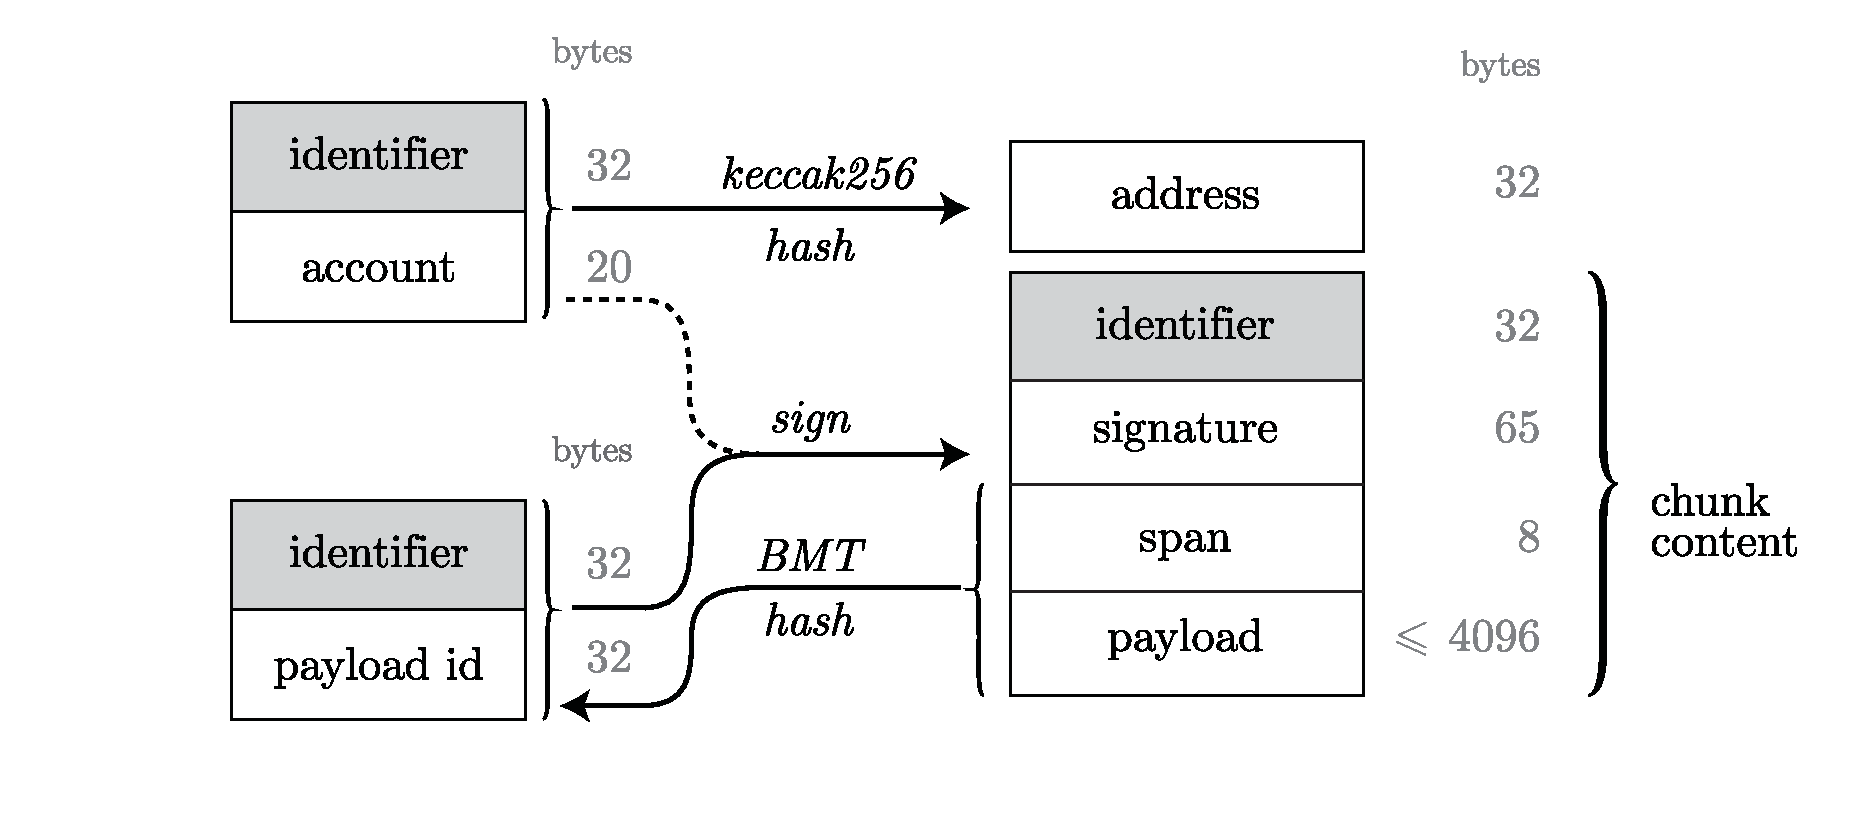
\includegraphics[width=\textwidth]{fig/single-owner-chunk.pdf}
   \caption[Single owner chunk\statusgreen]{Single owner chunk. The chunk content is composed of headers followed by an at most 4KB payload. The last header field is the 8-byte span prepended just like in content addressed chunks. The first two header fields provide single-owner attestation of integrity: an identifier and a signature signing off on the identifier and the BMT hash of span and payload. The address is the hash of the ID and the signer account.}
   \label{fig:single-owner-chunks}
\end{figure}

The validity of a \gloss{single owner chunk} is checked with the following process:

\begin{enumerate}
    \item Deserialise the chunk content into fields for identifier, signature, and payload.
    \item Construct the expected plain text composed of the identifier and the \gloss{BMT hash} of the payload.
    \item Recover the owner's address from the signature using the plain text.
    \item Check the hash of the identifier and the owner (expected address) against the chunk address.
\end{enumerate}

Single owner chunks offer a virtual partitioning of part of the address space into subspaces associated with the single owner. Checking their validity is actually an authentication verifying that the owner has write access to the address with the correct identifier.

As suggested by the span and the length of the payload, a single owner chunk can encapsulate a regular content addressed chunk. Anyone can simply reassign a regular chunk to an address in their subspace designated by the identifier (see also \ref{sec:notification-requests}).


It should be noted that the notion of integrity is somewhat weaker for single owner chunks than in the case of content addressed chunks: After all, it is, in principle, possible to assign and sign any payload to an identifier. Nonetheless, given the fact that the chunk can only be created by a single owner (of the private key that the signature requires), it is reasonable to expect uniqueness guarantees because we hope the node will want to comply with application protocols to get the desired result. However, if the owner of the private key signs two different payloads with the same identifier and uploads both chunks to Swarm, the behaviour of the network is unpredictable. Measures can be taken to mitigate this in layer (3) and are discussed later in detail in \ref{sec:feed-integrity}.

With two types of chunks, integrity is linked to collision-free hash digests, derived from either a single owner and an arbitrary identifier attested by a signature or directly from the content. This justifies the resolution of the DISC acronym as \emph{data integrity through signing or content address}.

\subsection{Chunk encryption\statusgreen}\label{sec:chunk-encryption}

Chunks should be encrypted by default. Beyond client needs for confidentiality, encryption has two further important roles. (1) Obfuscation of chunk content by encryption provides a degree of \gloss{plausible deniability}; using it across the board makes this defense stronger. (2) The ability to choose arbitrary encryption keys together with the property of uniform distribution offer predictable ways of \gloss{mining chunks}, i.e.,\ generating an encrypted variant of the same content so that the resulting chunk address satisfies certain constraints, e.g. is closer to or farther away from a particular address. This is an important property used in (1) price arbitrage (see \ref{sec:pricing}) and (2) efficient utilisation of postage stamps (see \ref{sec:postage-stamps}).


\begin{figure}[htbp]
    \centering
    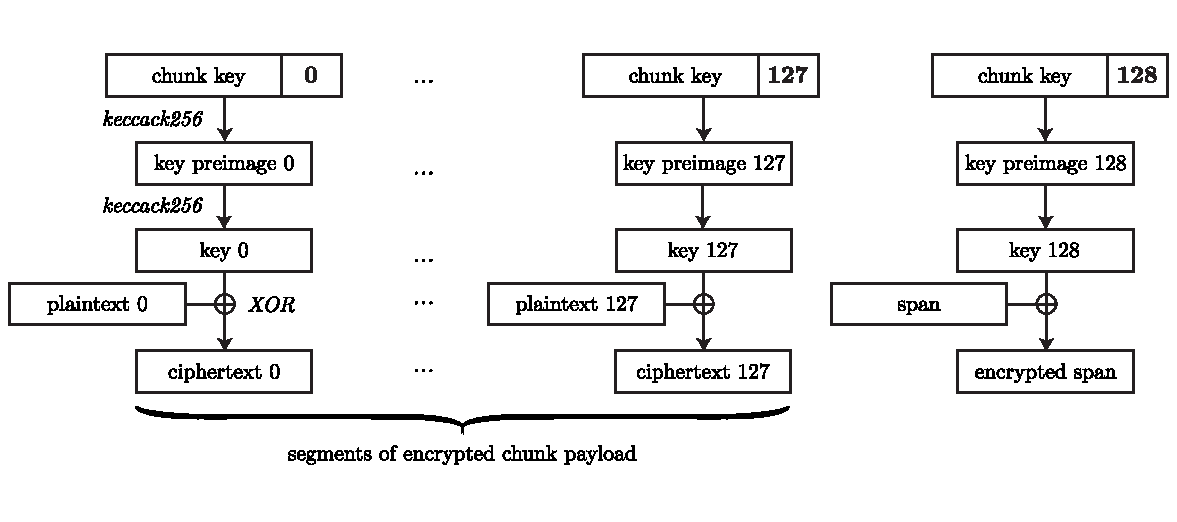
\includegraphics[width=\textwidth]{fig/chunk-encryption.pdf}
    \caption[Chunk encryption in Swarm \statusgreen]{Chunk encryption in Swarm. Symmetric encryption with a modified counter-mode block cipher. The plaintext input is the content padded with random bytes to 4 kilobytes. The span bytes are also encrypted as if they were continuations of the payload.}
    \label{fig:chunk-encryption}
\end{figure}


Chunks shorter than 4 kilobytes are padded with random bytes (generated from the chunk encryption seed). The full chunk plaintext is encrypted and decrypted using a XOR-based block cipher seeded with the corresponding symmetric key. In order not to increase the attack surface by introducing additional cryptographic primitives, the block cipher of choice is using Keccak256 in counter mode, i.e. hashing together the key with a counter for each consecutive segment of 32 bytes. In order to allow selective disclosure of individual segments that are part of an encrypted file, yet leak no information about the rest of the file, we add an additional step of hashing to derive the encryption key for a segment within the chunk. This scheme is easy and cheap to implement in the \gloss{EVM}, lending itself to use in smart contracts containing the plaintext of encrypted Swarm content. 

The prepended metadata encoding the chunk span is also encrypted as if it was a continuation of the chunk, i.e. with counter 128. Encrypted chunk content is hashed using the \gloss{BMT hash} digest just as unencrypted ones are. The fact that a chunk is encrypted may be guessed from the \gloss{span value}, but apart from this, in the network layer, encrypted chunks behave in exactly the same way as unencrypted ones.

\glossupperplural{single owner chunk} can also be encrypted, which simply means that they wrap an encrypted regular chunk. Therefore, their payload and span reflect the chunk content encryption described above, the hash signed with the identifier is the \gloss{BMT hash} of the encrypted span and payload, i.e. the same as that of the wrapped chunk.

\subsection{Redundancy by replication\statusgreen}\label{sec:redundancy-by-local-replication}

It is important to have a resilient means of requesting data. To achieve this, Swarm implements the approach of defence in depth. In the case that a request fails due to a problem with forwarding, one can retry the request with another peer. Alternatively, to guard against these occurrences, a node can initiate concurrent \glossplural{retrieve request} right away. However, such fallback options are not available if the single last node that stores the chunk drops out from the network. Therefore, redundancy is of major importance to ensure data availability. If the closest node is the only storer of the requested data and it drops out of the network, then there is no way to retrieve the content. This basic scenario is handled by ensuring that each set of \gloss{nearest neighbours} hold replicas of each chunk that is closest to any one of them, duplicating the storage of chunks and therefore providing data redundancy. 

\subsubsection{Size of nearest neighbourhoods}

If the Kademlia connectivity is defined over storer nodes, then in a network with Kademlia topology there exists a depth $d$ such that (1) each \gloss{proximity order bin} less than $d$ contains at least $k$ storer peers, and (2) all \glossplural{storer node} with \gloss{proximity order} $d$ or higher are actually connected peers. In order to ensure data redundancy, we can add to this definition a criterion that (3) the nearest neighbourhood defined by $d$ must contain at least $r$ peers.

Let us define \gloss{neighbourhood size} $\mathit{NHS}_x(d)$  as the cardinality of the neighbourhood defined by depth $d$ of node $x$. 
Then, a node has Kademlia connectivity with redundancy factor $r$ if there exists a depth $d$ such that (1) each proximity order bin lower than $d$ contains at least $k$ storer peers ($k$ is the bin density parameter, see \ref{sec:bindensity}), and (2) all storer nodes with proximity order $d$ or higher are actually connected peers, and (3) $\mathit{NHS}_x(d)\geq r$.

We can then take the highest depth $d'$ such that (1) and (2) are satisfied. Such a $d$ is guaranteed to exist and the \glossupper{hive protocol} is always able to bootstrap it. As we decrease $d'$, the number of distinct neighbourhoods grow proportionally, so for any redundancy parameter not greater than the network size $r\leq N=\mathit{NHS}_x(0)$, there will be a highest $0<d_r\leq d'$ such that $\mathit{NHS}_x(d_r)\geq r$. Therefore, \gloss{redundant Kademlia connectivity} is always achievable. 



For a particular redundancy, the area of the fully connected neighbourhood defines an \gloss{area of responsibility}. The proximity order boundary of the area of responsibility defines a \gloss{radius of responsibility} for the node. A storer node is said to be \emph{responsible} for (storing) a chunk if the chunk address falls within the node's radius of responsibility.

It is already instructive at this point to show neighbourhoods and how they are structured, see Figure \ref{fig:nearest-neighbours}. 

\begin{figure}[htbp]
   \centering
   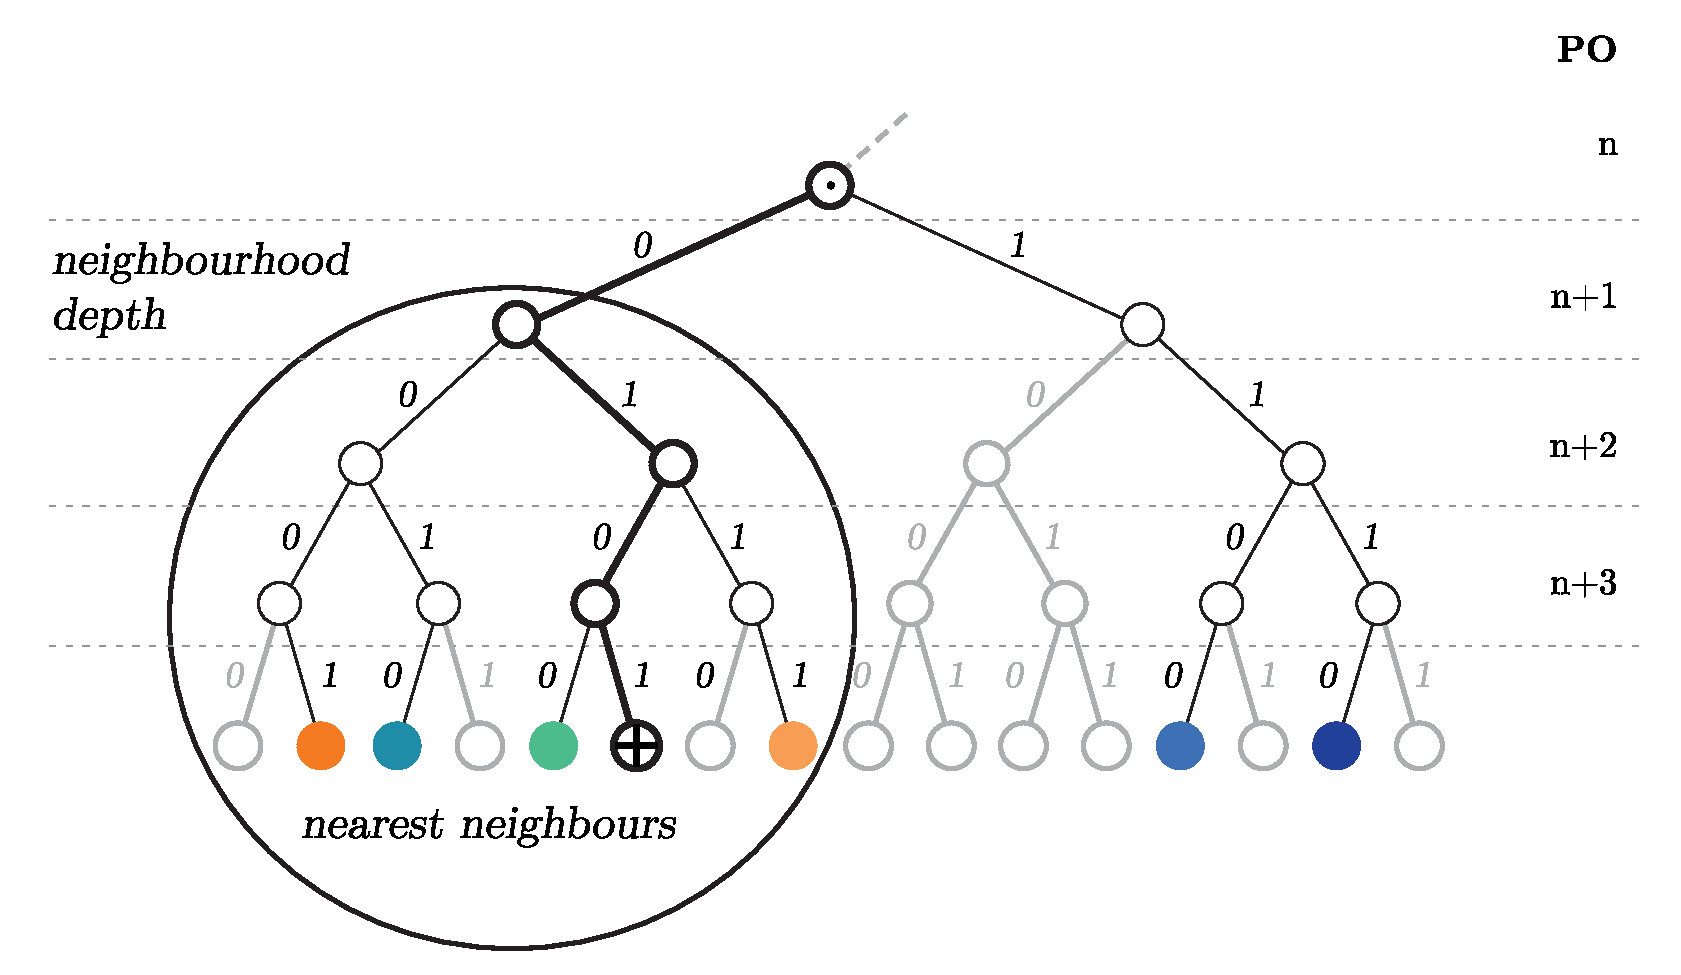
\includegraphics[width=\textwidth]{fig/nearest-neighbours-2.pdf}\\
   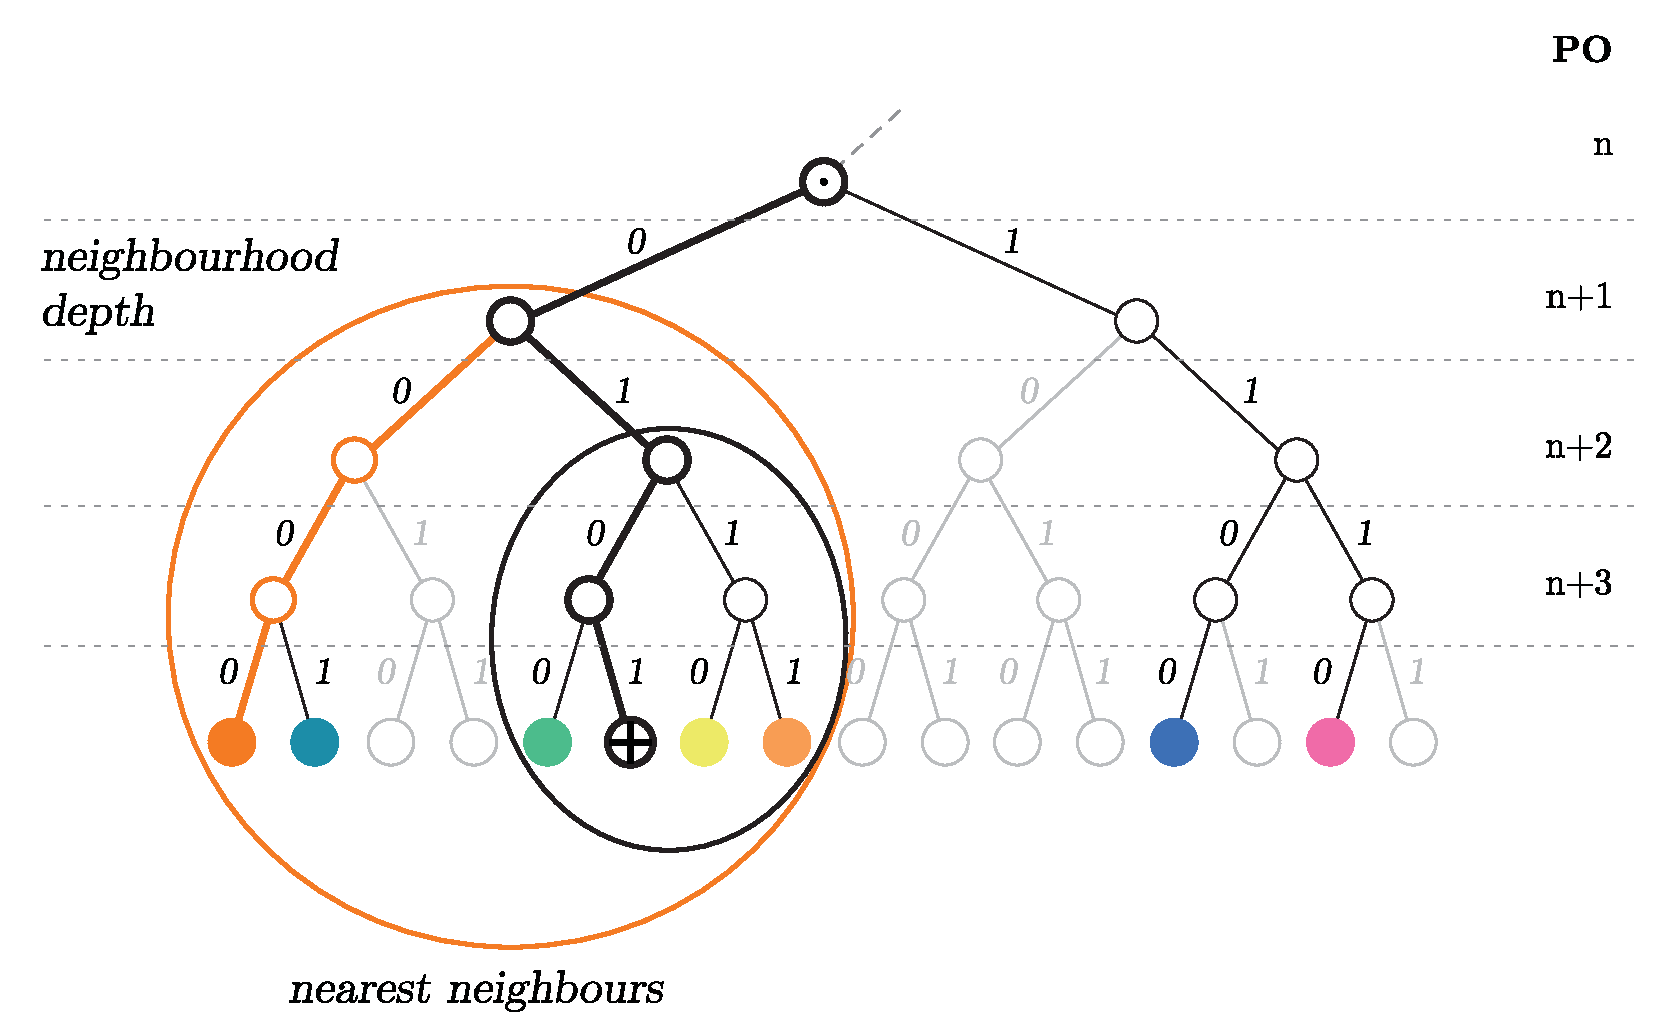
\includegraphics[width=\textwidth]{fig/asymmetric-nodes2.pdf}
   \caption[Nearest neighbours \statusgreen]{Nearest neighbours. \textbf{Top}: Each PO defines a neighbourhood, the neighbourhood depth of the node (black circle) is defined as the highest PO such that the neighbourhood has at least R=4 peers (redundancy parameter) and all shallower bins are non-empty. \textbf{Bottom}: An asymmetric neighbourhood. Nearest neighbours of the orange node include the black node but not the other way round.}
   \label{fig:nearest-neighbours}
\end{figure}


\subsubsection{Redundant retrievability}

A chunk is said to have \gloss{redundant retrievability} with degree $r$ if it is retrievable and would remain so even after any $r$ nodes responsible for it leave the network. The naive approach presented so far requiring the single closest node to keep the content can be interpreted as degree zero retrievability. If nodes in their area of responsibility fully replicate their content (see \ref{sec:pull-syncing}), then every chunk in the Swarm DISC is redundantly retrievable with degree $r$. Let us take the node $x$ that is closest to a chunk $c$. Since it has Kademlia connectivity with redundancy $r$, there are $r+1$ nodes responsible for the chunk in a neighbourhood fully connected and replicating content. After $r$ responsible nodes drop out, there is just one node remaining which still has the chunk. However, if Kademlia connectivity is maintained as the $r$ nodes leave, this node will continue to be accessible by any other node in the network, and therefore the chunk is still retrievable. Now, for the network to ensure that all chunks remain redundantly retrievable with degree $r$, the nodes comprising the new neighbourhood formed due to the reorganising of the network must respond by re-syncing their content to satisfy the protocol's replication criteria. This is called the guarantee of \gloss{eventual consistency}.

\subsubsection{Resource constraints}

Let us assume then that (1) the forwarding strategy that relays requests along \glossplural{stable node} and (2) the storage strategy that each node in the nearest neighbourhood (of $r$ storer nodes) stores all chunks whose addresses fall within their radius of responsibility. As long as these assumptions hold, each chunk is retrievable even if $r$ storer nodes drop offline simultaneously. As for (2), we still need to assume that every node in the nearest neighbour set can store each chunk. Realistically, however, all nodes have resource limitations. With time, the overall amount of distinct chunks ever uploaded to Swarm will increase indefinitely. Unless the total storage capacity steadily increases, we should expect that the nodes in Swarm are able to store only a subset of chunks. Some nodes will reach the limit of their storage capacity and therefore face the decision whether to stop accepting new chunks via syncing or to make space by deleting some of their existing chunks. 

The process that purges chunks from their local storage is called \gloss{garbage collection}. The process that dictates which chunks are chosen for garbage collection is called the \gloss{garbage collection strategy}. For a profit-maximizing node, it holds that it is always best to garbage-collect the chunks that are predicted to be the least profitable in the future and, in order to maximize profit, it is desired for a node to get this prediction right (see \ref{sec:postage-stamps}). So, in order to factor in these capacity constraints, we will introduce the notion of \gloss{chunk value} and modify our definitions using the minimum value constraint:

In Swarm's DISC, at all times, there is a chunk value $v$ such that every chunk with a value greater than $v$ is both retrievable and eventually (after syncing) redundantly retrievable with degree $r$. 

This value ideally corresponds to the relative importance of preserving the chunk that uploaders need to indicate. In order for storer nodes to respect it, the value should also align with the profitability of a chunk and is therefore expressed in the pricing of uploads (see \ref{sec:depths}).

% \subsection{}\label{sec:}

\section{Push and pull: chunk retrieval and syncing\statusgreen}\label{sec:push-and-pull}
\green{}
In this section, we demonstrate how chunks actually move around in the network: How they are pushed to the storer nodes in the neighbourhood they belong to when they are uploaded, as well as how they are pulled from the storer nodes when they are downloaded.

\subsection{Retrieval\statusgreen}\label{sec:retrieval}

In a distributed chunk store, we say that a chunk is an \gloss{accessible chunk} if a message is routable between the requester and the node that is closest to the chunk. Sending a retrieve request message to the chunk address will reach this node.  Because of \gloss{eventual consistency}, the node closest to the chunk address will store the chunk. Therefore, in a \gloss{DISC} distributed chunk store with healthy Kademlia topology, all chunks are always accessible for every node.

\subsubsection{Chunk delivery}

For retrieval, accessibility needs to be complemented with a process to have the content delivered back to the requesting node, preferably using only the chunk address. There are at least three alternative ways to achieve this (see Figure \ref{fig:chunk-delivery}):

\begin{enumerate}
    \item \gloss{direct delivery} -- The chunk delivery is sent via a direct underlay connection. 
    \item \gloss{routed delivery} -- The chunk delivery is sent as message using routing.
    \item \gloss{backwarding} -- The chunk delivery response simply follows the route along which the request was forwarded, just backwards all the way to the originator.
\end{enumerate}


\begin{figure}[htbp]
   \centering
   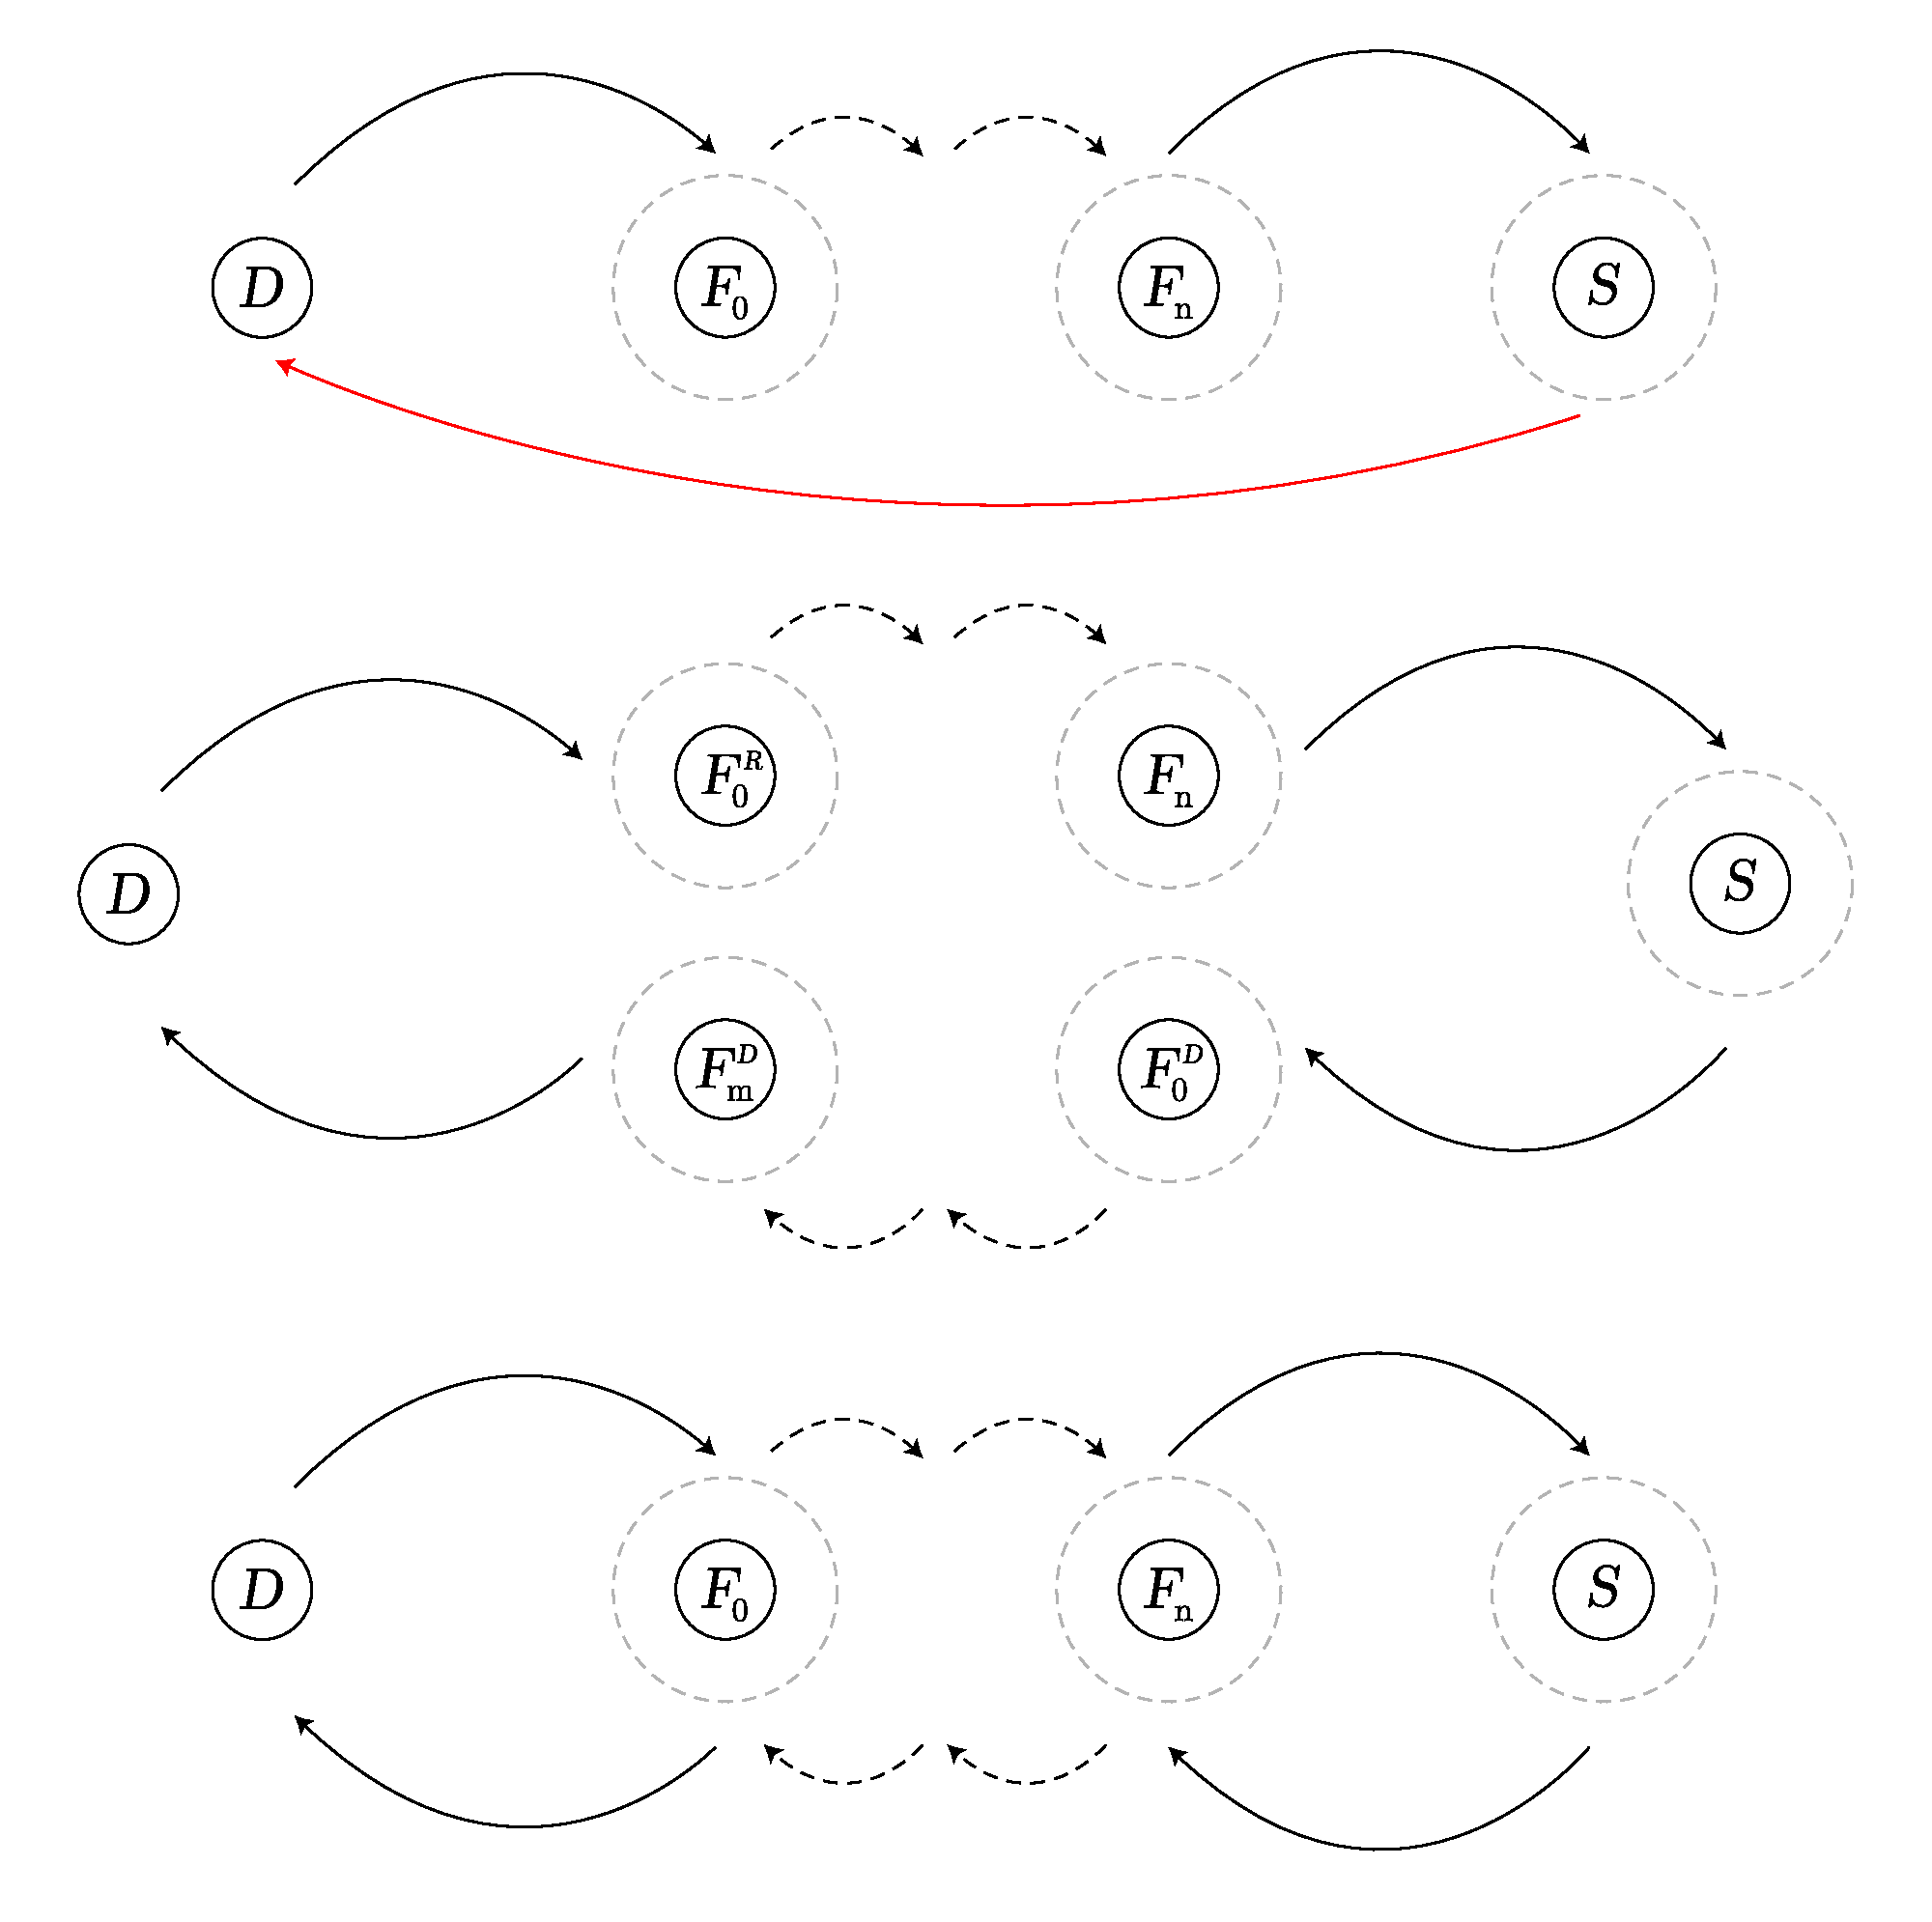
\includegraphics[width=\textwidth]{fig/chunk-delivery.pdf}
   \caption[Alternative ways to deliver chunks: direct, routed and backward \statusgreen]{Alternative ways to deliver chunks. \textbf{Top:} \emph{direct delivery}: via direct underlay connection. \textbf{Centre:} \emph{routed delivery}: chunk is sent using Kademlia routing. \textbf{Bottom:} \gloss{backwarding} re-uses the exact peers on the path of the request route to relay the delivery response.}
   \label{fig:chunk-delivery}
\end{figure}

Firstly, using the obvious direct delivery, the chunk is delivered in one step via a lower-level network protocol. This requires an ad-hoc connection with the associated improvement in latency traded off for worsened security of privacy.%
%
\footnote{Beeline delivery has some merit, i.e. bandwidth saving and better latency, so we do not completely rule out the possibility of implementing it. 
}
Secondly, using routed delivery, a chunk is delivered back to its requestor using ad-hoc routing as determined from the storer's perspective at the time of sending it. Whether direct or routed, allowing deliveries routed independently of the request route presupposes that the requestor's address is (at least partially) known by the storer and routing nodes. Consequently, these methods disclose information that can identify the requestor. However, with forwarding--backwarding Kademlia this is not necessary: The storer node responds back to their requesting peer with the delivery, while intermediate \glossplural{forwarding node} remember which of their peers requested what chunk. When the chunk is delivered, they pass it on back to their immediate requestor, and so on until it eventually arrives at the node that originally requested it. In other words, the chunk delivery response simply follows the request route back to the originator (see Figure \ref{fig:request-response}).  Since it is the reverse of the forwarding, we can playfully call this \gloss{backwarding}. Swarm uses this option, which makes it possible to disclose no requestor identification in any form, and thus Swarm implements completely \gloss{anonymous retrieval}. 

\begin{figure}[htbp]
   \centering
   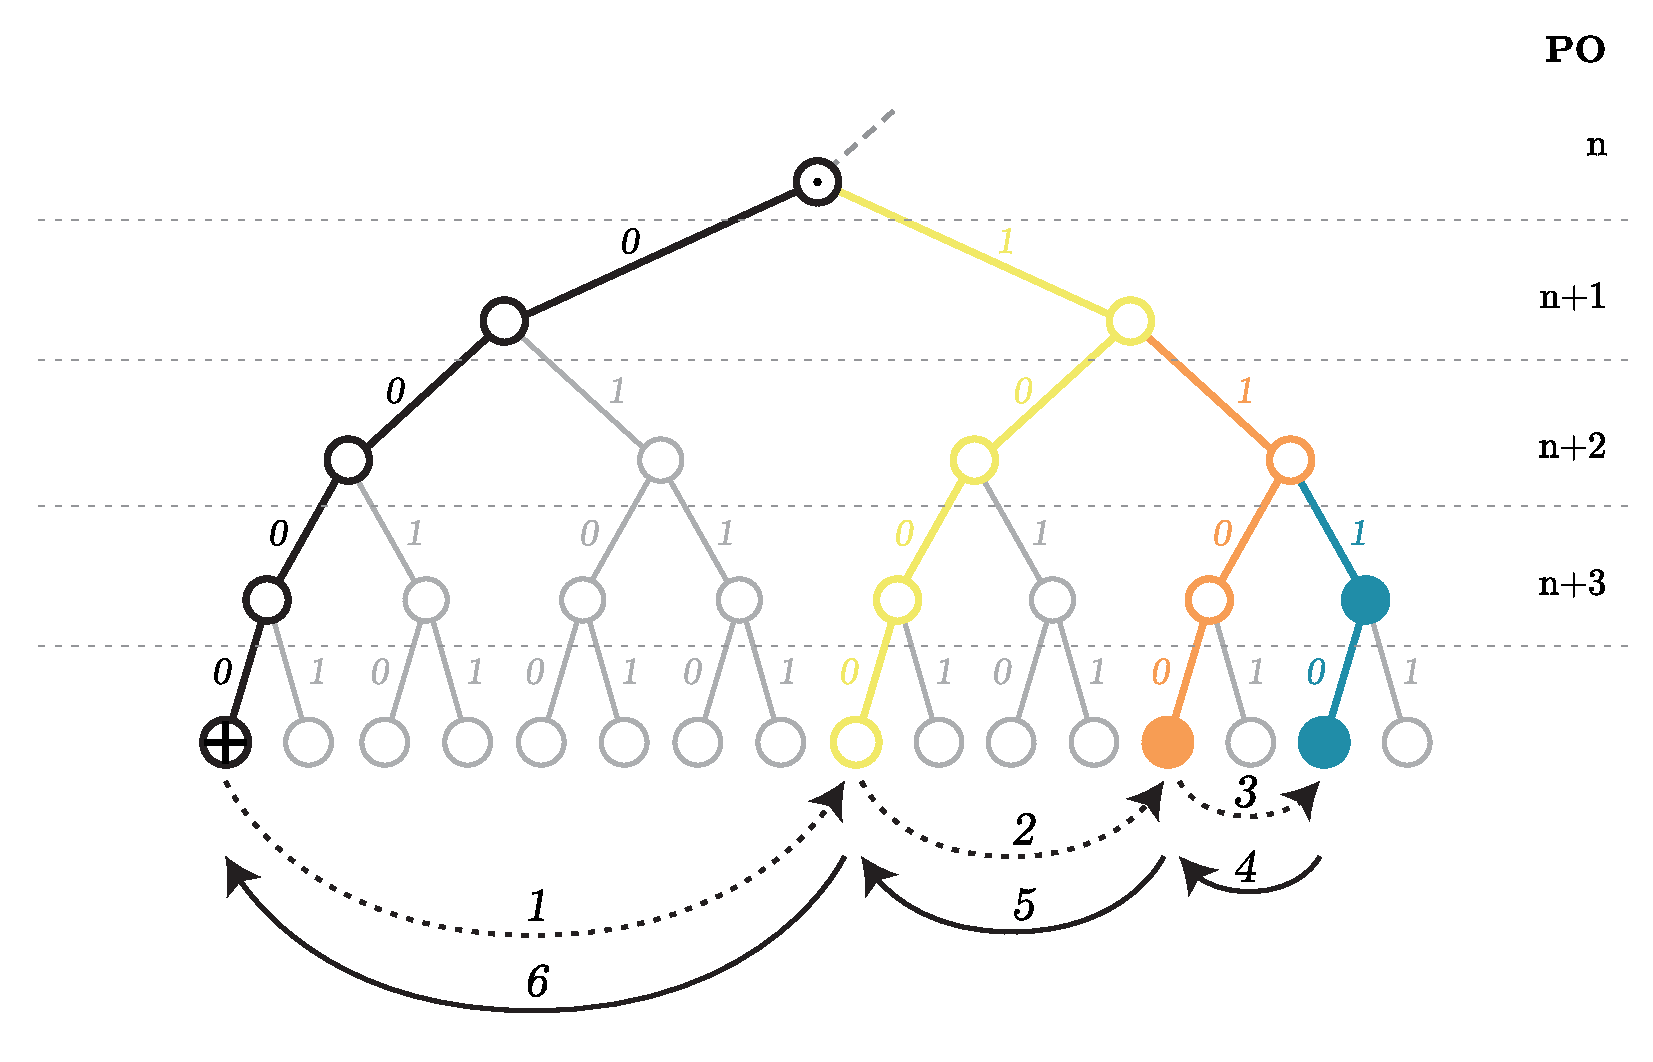
\includegraphics[width=\textwidth]{fig/request-response-forwarding.pdf}
   \caption[Backwarding: a pattern for anonymous request-response round-trips in forwarding Kademlia \statusgreen]{Backwarding: pattern for anonymous request--response round-trips in forwarding Kademlia. Here a node with overlay address $...0000...$ sending a request to target $....1111...$ to which the closest online node is $...1110...$ The leading ellipsis represents the prefix shared by the requestor and target and has a length of $n$ bits. The trailing ellipsis represents part of the address that is not relevant for routing as at that depth nodes are already unique. The request uses the usual Kademlia forwarding, but the relaying nodes on the way remember the peer the request came from so that when the response arrives, they can \emph{backward} it (i.e.\ pass it back) along the same route.}
   \label{fig:request-response}
\end{figure}

Ensuring requestor anonymity by default in the retrieval protocol is a crucial feature that Swarm insists upon. This feature aims to safeguard user privacy and enables censorship-resistant access.

\begin{figure}[htbp]
   \centering
   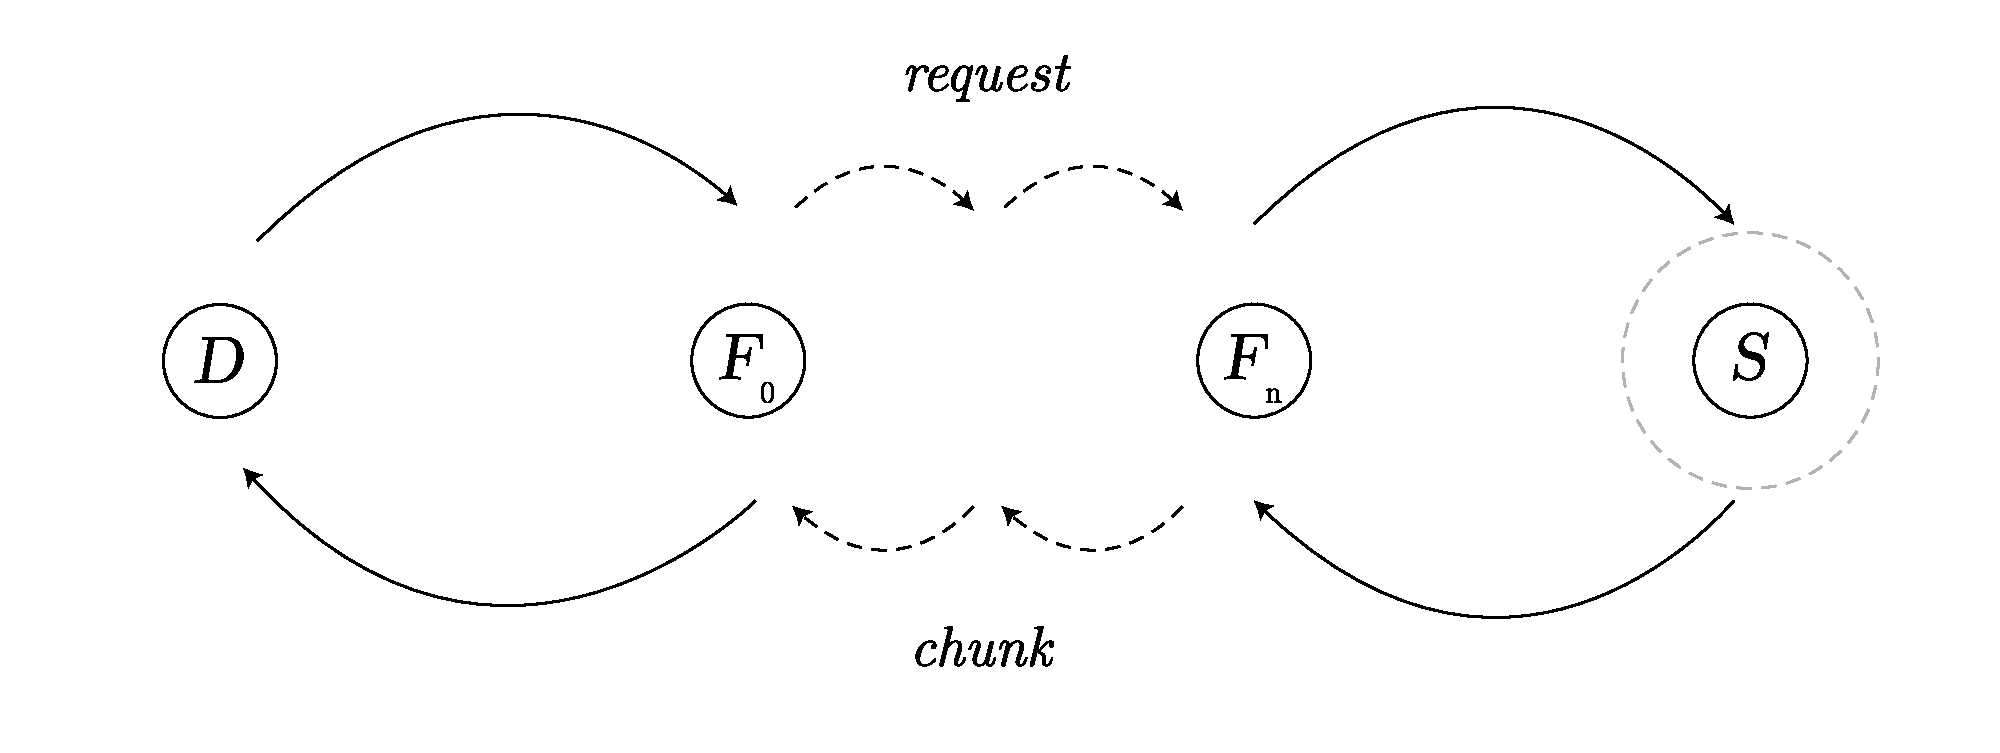
\includegraphics[width=\textwidth]{fig/retrieval.pdf}
   \caption[Retrieval \statusgreen]{Retrieval. Node $D$ (Downloader) sends a retrieve request to the chunk's address. Retrieval uses forwarding Kademlia, so the request is relayed via forwarding nodes $F_0$, ..., $F_n$ all the way to node $S$, the storer node closest to the chunk address. The chunk is then delivered by being passed back along the same route to the downloader.}
   \label{fig:retrieval}
\end{figure}

The generic solution of implementing retrieval by backwarding as depicted in Figure \ref{fig:retrieval} has further benefits relating to spam protection, scaling and incentivisation, which will be discussed in the remainder of this section.

\subsubsection{Protection against unsolicited chunks}

In order to remember requests, the \gloss{forwarding node} needs to allocate resources that come with a certain cost (they occupy space in memory). The requests that are not followed by a corresponding delivery should eventually be garbage collected, so there needs to be a defined time period during which they are active. Downstream peers also need to be informed about the timeout of this request. This makes sense, since the originator of the request will want to attach a time-to-live duration to the request to indicate how long it will wait for a response.  

Sending unsolicited chunks is an offence as it can lead to \gloss{denial of service (DoS)}. By remembering a request, nodes are able to recognise unsolicited chunk deliveries and penalise the peers sending them. Chunks that are delivered after the request expires will be treated as unsolicited. Since there may be some discrepancy assessing the expiry time between nodes, there needs to be some tolerance for unsolicited chunk deliveries, but if they go above a particular (but still small) percentage of requests forwarded, the offending peer is disconnected and blacklisted. Such local sanctions are the easiest and simplest way to incentivise adherence to the protocol (see \ref{sec:sanctions}). 

\subsubsection{Re-requesting}

There is the potential for a large proportion of Swarm nodes to not be always stably online. Such a high churn situation would be problematic if we used the naive strategy of forwarding requests to any one closer node: If a node on the path were to go offline before delivery is completed, then the request-response round trip is broken, effectively rendering the chunk requested not retrievable. Commitment to pay for a chunk is considered void if the connection to the requested peer is dropped, so there is no harm in re-requesting the chunk from another node.


\subsubsection{Timeout vs not found}

Note that in Swarm there is no explicit negative response for chunks not being found. In principle, the node that is closest to the retrieved address can determine the absence of a chunk at that address and could issue a "not found" response. However, this is not desirable for the following reason: While the closest node to a chunk can verify its absence from its expected location in the network, nodes further away from the chunk cannot reliably conclude the same. They lack first-hand verification, and any positive evidence regarding the chunk's retrievability obtained later can be retrospectively plausibly deniable. 

All in all, as long as delivery has the potential to create earnings for the storer, the best strategy is to keep a pending request open until it times out and be prepared in case the chunk should appear. There are several ways the chunk could arrive after the request: (1) syncing from existing peers (2) appearance of a new node or (3) if a request precedes upload, e.g. the requestor has already "subscribed" to a single owner address (see \ref{sec:messaging}) to decrease latency of retrieval. This is conceptually different from the usual server-client based architectures where it makes sense to expect a resource to be either on the host server or not. 
 

\subsubsection{Opportunistic caching}

Using backwarding for chunk delivery responses to retrieve requests also enables \gloss{opportunistic caching}, where a \gloss{forwarding node} receives a chunk and the chunk is then saved in case it will be requested again. This mechanism is crucial in ensuring that Swarm scales the storage and distribution of popular content automatically (see \ref{sec:caching}).

\subsubsection{Incentives}

So far, we have shown that by using the retrieval protocol and maintaining Kademlia connectivity, nodes in the network are capable of retrieving chunks. However, since forwarding is expending a scarce resource (bandwidth), without providing the ability to account for this bandwidth use, network reliability will be contingent on the proportion of freeriding and altruism. To address this, in Section \ref{sec:incentivisation} we will outline a system of economic incentives that align with the desired behaviour of nodes in the network. When these profit-maximising strategies are employed by node operators, they give rise to emergent behaviour that is beneficial for users of the network as a whole.
 
\subsection{Push syncing\statusgreen}\label{sec:push-syncing}
 
In the previous sections, we presented how a network of nodes maintaining a Kademlia overlay topology can be used as a distributed chunk store and how Forwarding Kademlia routing can be used to define a protocol for retrieving chunks.
When discussing retrieval, we assumed that chunks are located with the node whose address is closest to theirs. This section describes the protocol responsible for realising this assumption: ensuring delivery of the chunk to its prescribed storer after it has been uploaded to any arbitrary node.

This network protocol, called \gloss{push syncing}, is analogous to chunk retrieval: First, a chunk is relayed to the node closest to the chunk address via the same route as a retrieval request would be, and then in response a \gloss{statement of custody receipt} is passed back along the same path (see Figure \ref{fig:push-syncing}). The statement of custody sent back by the storer to the \gloss{uploader} indicates that the chunk has reached the neighbourhood from which it is universally retrievable. By tracking these responses for each constituent chunk of an upload, uploaders can make sure that their upload is fully retrievable by any node in the network before sharing or publishing the address of their upload. Keeping this count of chunks push-synced and receipts received serves as the back-end for a \emph{progress bar} that can be displayed to the uploader to give feedback of the successful propagation of their data across the network (see \ref{sec:upload}).


\begin{figure}[htbp]
   \centering
   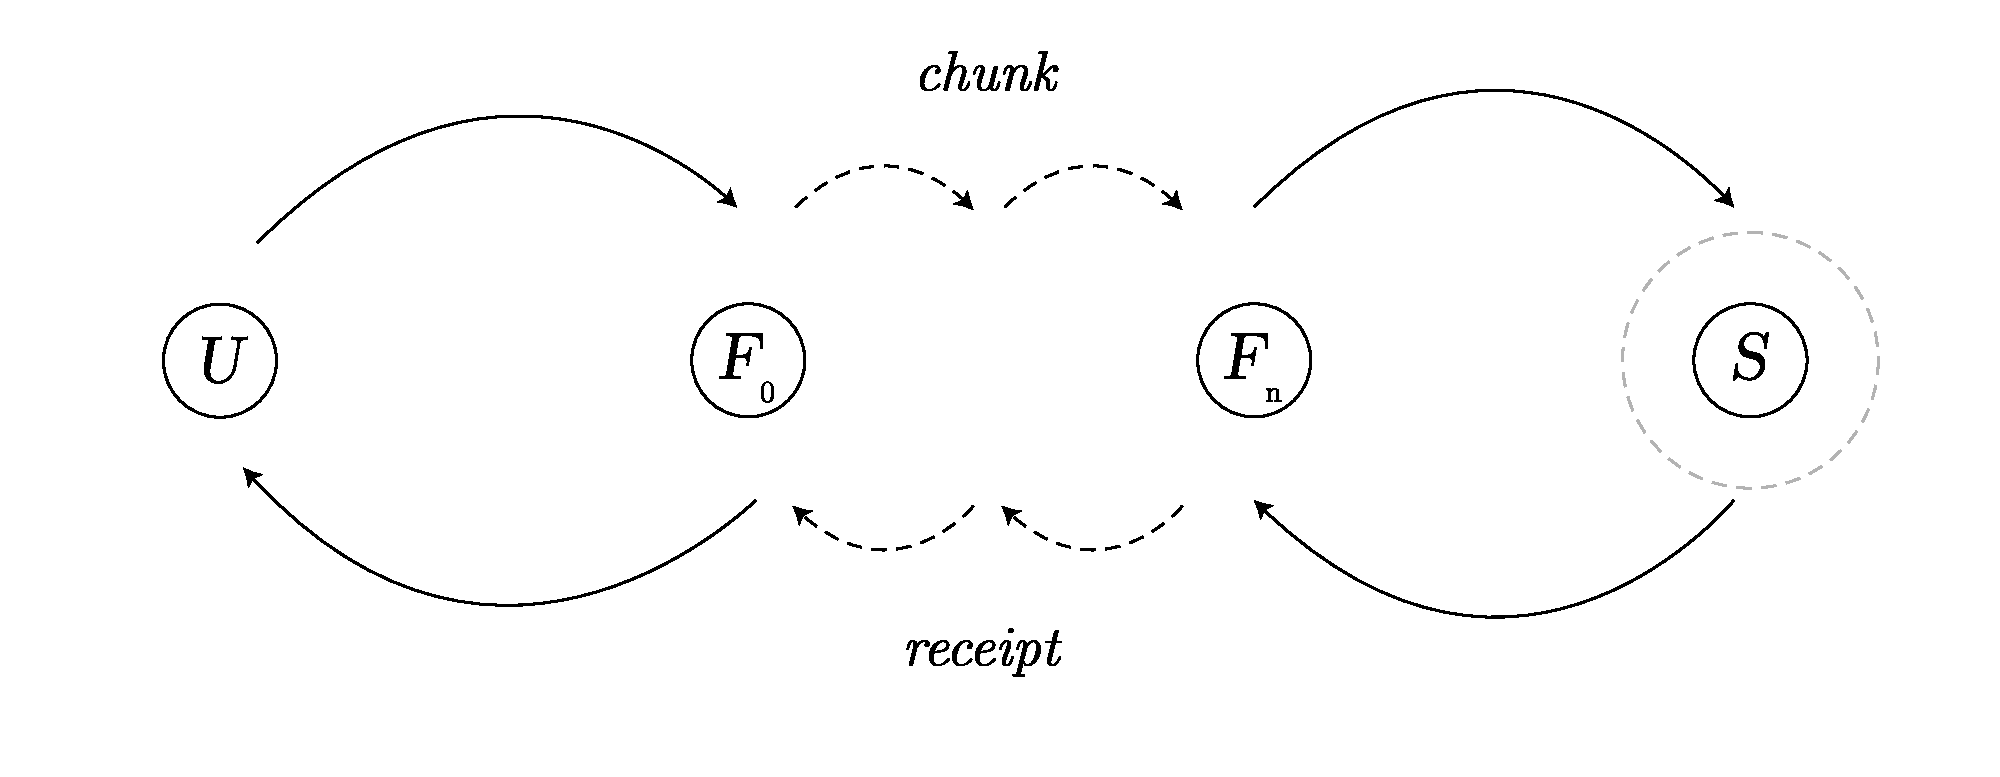
\includegraphics[width=\textwidth]{fig/push-sync.pdf}
   \caption[Push syncing \statusgreen]{Push syncing. Node $U$ (Uploader) push-syncs a chunk to the chunk's address. Push-sync uses forwarding, so the chunk is relayed via forwarding nodes $F_0$, ..., $F_n$ all the way to node $S$, the storer node closest to the chunk address (the arrows represent transfer of the chunk  via direct peer-to-peer connection). A statement of custody receipt signed by $S$ is then passed back along the same route as an acknowledgment to the uploader.}
   \label{fig:push-syncing}
\end{figure}

Statements of custody are signed by the nodes that claim to be the closest to the address. 
Similarly to downloaders in the retrieval protocol, the identity of uploaders can also remain hidden, hence forwarding Kademlia can implement \gloss{anonymous uploads}.

Another similarity is that in order to allow backwarding for responses, nodes should remember which peer sent a particular chunk. This record should persist for a short period while the statement of custody responses are expected. When this period ends, the record is removed. A statement of custody not matching a record is considered unsolicited and is allowed only up to a small percentage of all push-sync traffic with a peer. Going above this tolerance threshold is sanctioned with disconnection and blacklisting (see \ref{sec:sanctions}).

In this section, we described how the logistics of chunk uploads can be organised with a network protocol using Forwarding Kademlia routing with response backwarding. However, this solution is not complete until it is secured with aligned incentives: The strategy to follow this protocol should be incentivised and DoS abuse should be disincentivised. These are discussed later in detail in \ref{sec:postage-stamps} and \ref{sec:push-sync-incentives}).

\subsection{Pull syncing\statusgreen}\label{sec:pull-syncing}

\glossupper{pull syncing} is the protocol that is responsible for the following two properties: 

\begin{itemize}
    \item \emph{eventual consistency} -- Syncing neighbourhoods as and when the topology changes due to churn or new nodes joining.
    \item \emph{maximum resource utilisation} -- Nodes can pull chunks from their peers to fill up their surplus storage.%
%
\footnote{Maximum storage utilisation may not be optimal in terms of the profitability of nodes. Put differently, storer nodes have an optimal storage capacity based on how often content is requested from them. This means that in practice, profit-optimised maximum utilisation of storage capacity requires operators to run multiple node instances.}
\end{itemize}

Pull syncing is node-centric as opposed to chunk-centric, i.e. it makes sure that a node's storage is filled if needed, as well as syncing chunks within a neighbourhood. When two nodes are connected, they will start syncing both ways so that on each peer connection there is bidirectional chunk traffic. The two directions of syncing are managed by distinct and independent \emph{streams}. In the context of a stream, the consumer of the stream is called \gloss{downstream peer} or client, while the provider is called the \gloss{upstream peer} or server. 

When two nodes connect and engage in \gloss{chunk synchronisation}, the upstream peer offers all the chunks it stores locally in a data stream per proximity order bin. To receive chunks closer to the downstream peer than to the upstream peer, a downstream peer can subscribe to the chunk stream of the proximity order bin that the upstream peer belongs to in their Kademlia table. If the peer connection is within the nearest neighbour depth $d$, the client subscribes to all streams with proximity order bin $d$ or greater. As a result, peers eventually replicate all chunks belonging to their area of responsibility.

A pull syncing server's behaviour is referred to as being that of a \gloss{stream provider} in the stream protocol. Nodes maintain a record of the time when they stored a chunk locally by indexing them with an ascending storage count known as the \gloss{bin ID}. For each proximity order bin, upstream peers offer to stream chunks in descending order of storage timestamp. As a result of syncing streams on each peer connection, a chunk can be synced to a downstream peer from multiple upstream peers. In order to save bandwidth by not sending data chunks to peers that already have them, the stream protocol implements a round-trip: Before sending chunks, the upstream peer presents a batch of chunks identified by their address. The downstream peer then responds with indicating which chunks from the offered batch they actually need (see Figure \ref{fig:pull-syncing}). Note that the downstream peer determines whether they have the chunk based on the chunk address. Thus, this method critically relies on the chunk integrity assumption discussed in \ref{sec:chunks}.


\begin{figure}[htbp]
   \centering
   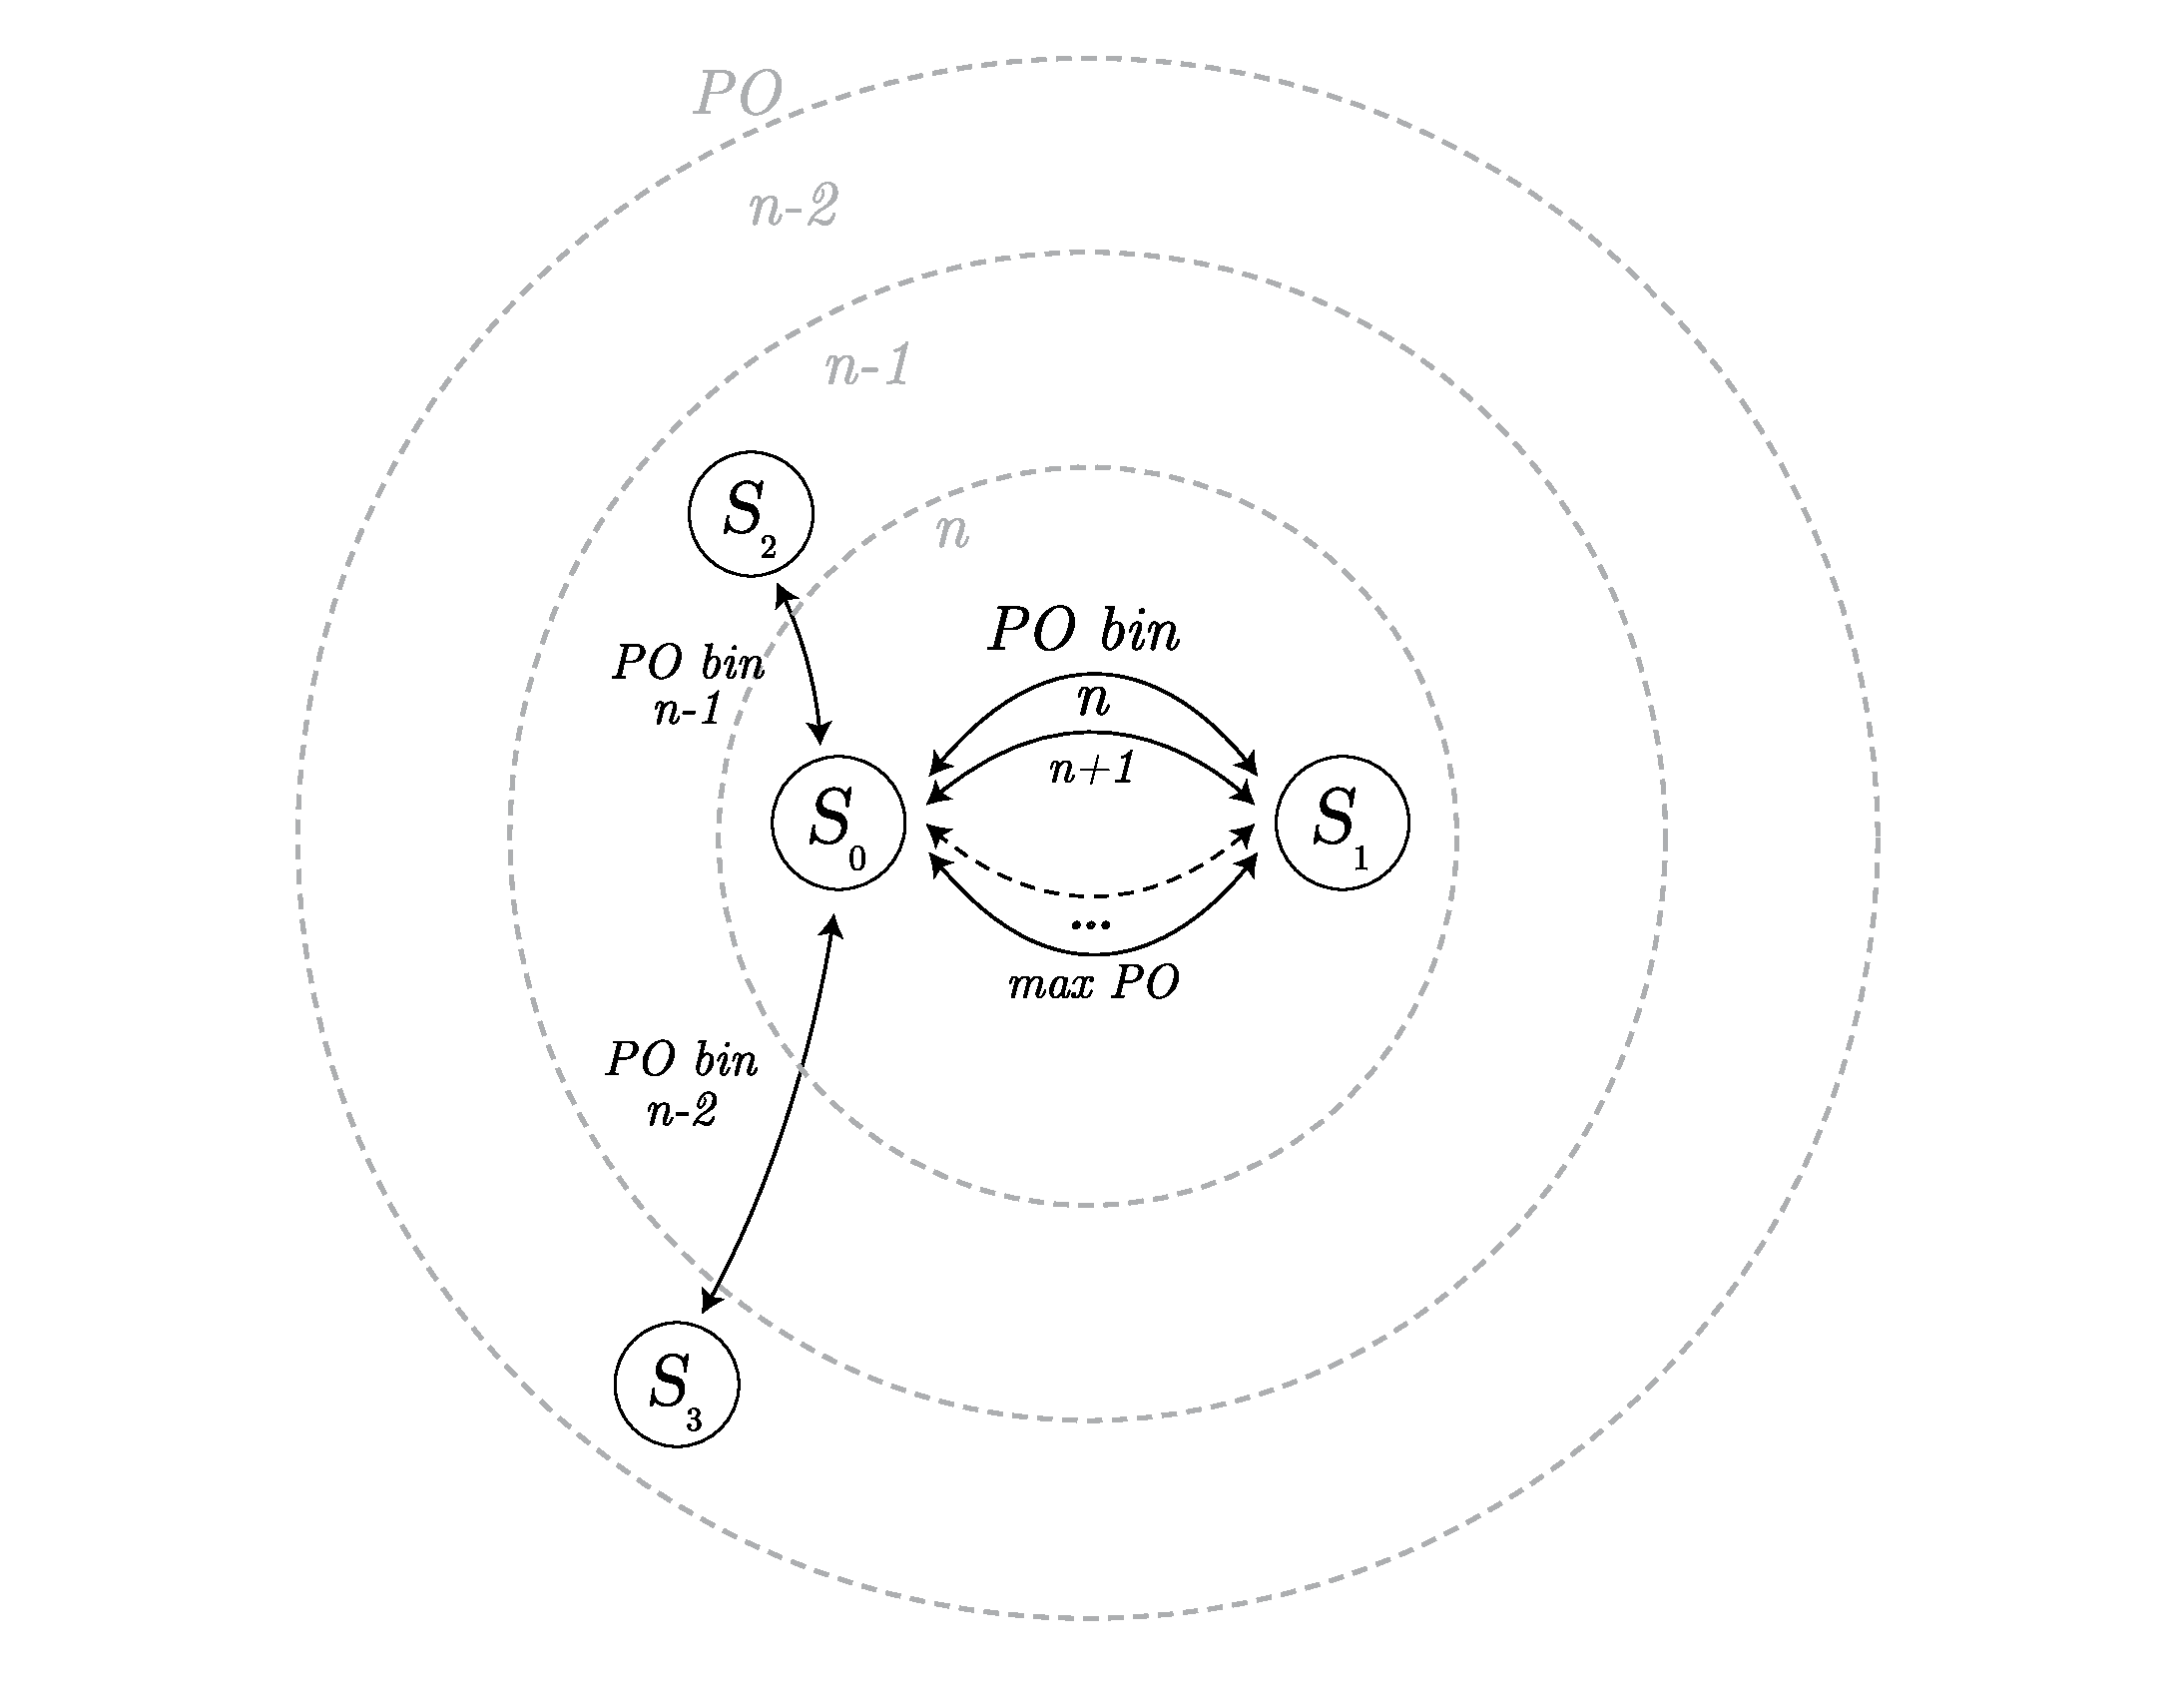
\includegraphics[width=\textwidth]{fig/pull-sync.pdf}
   \caption[Pull syncing \statusgreen]{Pull syncing. Nodes continuously synchronise their nearest neighbourhood. If they have free capacity, they also pull sync chunks belonging to shallower bins from peers falling outside the neighbourhood depth.}
   \label{fig:pull-syncing}
\end{figure}

In the context of a peer connection, a client is said to be \emph{synced} if it has synced all the chunks of the upstream peer. Note that due to disk capacity limitations, nodes must impose a value cutoff, and as such, "all chunks" reads as shorthand for "all chunks having a value greater than $v$" ($v$ is a constant ranking function, the origin of which is discussed later in \ref{sec:reserve}). In order for a node to promise they store all chunks with value greater than $v$, it is necessary for all its neighbours to have also stored all chunks greater than value $v$. In other words, nodes syncing inherit the maximum such value from among their storer peers. 

If chunks are synced in the order they are stored, this may not result in the node always having the most profitable (most often requested) chunks. Thus it may be advisable to sync chunks starting with the most popular ones according to upstream peers and finish syncing when storage capacity is reached. In this way, a node's limited storage will be optimised. Syncing and garbage collection are discussed further in \ref{sec:postage-stamps} and \ref{sec:depths}.

To conclude this section, we show how the criteria of \gloss{eventual consistency} are met in a healthy Swarm. Chunks found in the local store of any node will become retrievable after being synced to their storers. This is because as long as those as peers in the network pull chunks closer to them than to the upstream peer, each chunk travels a route that would also qualify as valid a forwarding path in the push-sync protocol. If new nodes are added and old nodes drop out, neighbourhoods change, but as long as local redundancy is high enough that churn can not render previously retrievable chunks non-retrievable, neighbourhoods eventually replicate their content and redundancy is restored. Consider the unlikely event that a whole new neighbourhood is formed and the nodes that originally held the content belonging to this neighbourhood end up outside of it, resulting in a temporary unavailability of those chunks. Even in this scenario, as long as there is a chain of nodes running pull-syncing streams on the relevant bins, redundant retrievability is eventually restored.

\subsection{Light nodes\statusgreen}
\label{sec:light}

The concept of a \gloss{light node} refers to a special mode of operation necessitated by poor bandwidth environments, e.g. mobile devices on low throughput networks or devices allowing only transient or low-volume storage.

A node is said to be light by virtue of not participating fully in the usual protocols detailed in the previous sections, i.e. retrieval, push syncing, or pull syncing. 

A node that has restricted bandwidth environment or in whatever way has limited capacity to maintain underlay connections is not expected to be able to forward messages conforming to the rules of Kademlia routing. This needs to be communicated to its peers so that they do not relay messages to it. 

As all protocols in Swarm are modular, a node may switch on or off any protocol independently (depending on capacity and earnings requirements). To give an example: a node that has no storage space available, but has spare bandwidth, may participate as a forwarding node only. Of course, while switching off protocols is technically feasible, a node must at all times take into account the fact that his peers expect a certain level of service if this is advertised and may not accept that some services are switched off and choose not to interact with that node. 

Since forwarding can earn revenue, these nodes may still be incentivised to accept retrieve requests. However, if the light node has Kademlia connectivity above proximity order bin $p$ (i.e. they  are connected to all storer nodes within their nearest neighbourhood of $r$ peers at depth $d$, and there is at least one peer in each of their proximity order bin from $p$ to $d$), they can advertise this and therefore participate in forwarding. 

When they want to retrieve or push chunks, if the chunk address falls into a proximity order bin where there are no peers, they can just pick a  peer in another bin. Though this may result in a spurious hop (where the proximity of the message  destination to the latest peer does not increase as a result of the relaying), the Kademlia assumption that routing can be completed in logarithmic steps still holds valid.

A node that is advertised as a storer/caching node is expected to store all chunks  above a certain value. In order to maintain consistency, they need to synchronise content within their area of responsibility, which requires them to run the pull-sync protocol. The same applies to aspiring storer nodes that come online with available storage and open up to pull-sync streams to fill their storage capacity. In the early stages of this, it does not make sense for a node to sync to other full storer nodes. However, it can still be useful for them to sync with other similar newcomer nodes, especially if storer nodes are maxing out on their bandwidth.

The crucial thing here is that for redundancy and hops to work, light nodes with incomplete, unsaturated Kademlia tables should not be considered by other peers when calculating the level of saturation of the network.


\chapter{Incentives}\label{sec:incentivisation}
The Swarm network comprises many independent nodes, running software which implements the Swarm protocol. It is important to realize that even though nodes run the same protocol, the emergent behavior of the network is not guaranteed by the protocol alone; as nodes are autonomous, they are essentially "free" to react in any way they desire to incoming messages of peers.
It is, however possible to make it profitable for a node to react in a way that is beneficial for the desired emergent behavior of the network, while making it costly to act in a way that is detrimental. Broadly speaking, this is achieved in Swarm by enabling a transfer of value from those nodes who are using the resources of the network (\glossplural{net user}) to those who are providing it (\glossplural{net provider}). 


\begin{figure}[htbp]
\centering
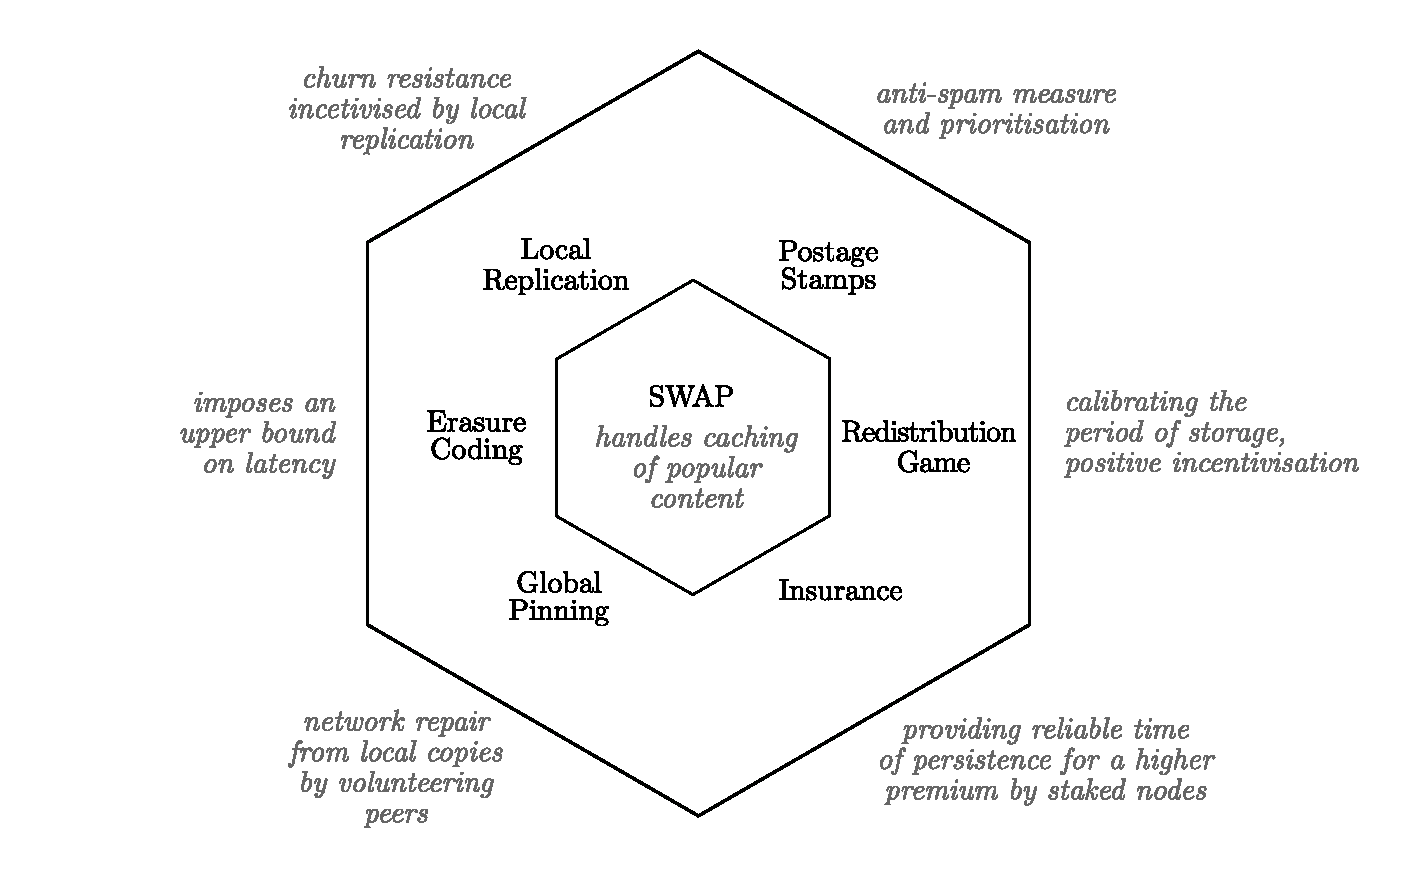
\includegraphics[width=\textwidth]{fig/incentive-design-3.pdf}
\caption[Incentive design \statusgreen]{Incentive design}
\label{fig:incentives}
\end{figure}

% The rest of this chapter is concerned with describing the desired emergent behaviour of the network (\ref{sec:emergent_behavior}), after which we describe the actions which incur costs and those that provide value (\ref{sec:cost_benefit}). Finally, we proceed by describing the incentive mechanisms which ensures that costs are borne as directly as possible by the initiator of the action, with benefits flowing to the nodes who provided the initiator with the expected outcome, ultimately facilitating the desired emergent behavior (see \ref{sec:incentive_mechanisms}).

% \section{Incentive design \statusred}
% \wip{foundational requirement + analysis} 
% \subsection{WIP Desired emergent behavior \statusred}\label{sec:emergent_behavior}
% \subsection{WIP Analysis on expected costs and benefits of actions \statusred}\label{sec:cost_benefit}
% \subsection{WIP Proposed incentive mechanisms \statusred}\label{sec:incentive_mechanisms}
% This section will constitute most of the sections which are already described below.


\section{Sharing bandwidth\statusgreen}

\green{}

\subsection{Incentives for serving and relaying\statusgreen}\label{sec:incentives-relaying}

\green{}

\subsubsection{Forwarding Kademlia and repeated dealings}

The retrieval of a chunk is ultimately initiated by someone accessing content, and therefore all costs related to this retrieval should be borne by them. While paid retrievals may not sound like a popular idea when today's web is "free", many of the problems with the current web stems from consumers' inability to share the costs of hosting and distribution with content publishers directly. In principle, the retrieval of a chunk can be perceived as a functional unit where the storer acts as a service provider and the requestor as consumer. The provider renders a service to the consumer, and in return, the consumer should provide compensation. Such a direct transaction would normally require that transactors are known to each other, so if we are to maintain the anonymity requirement on downloads, we must conceptualise compensation in a novel way. 

As we use forwarding Kademlia, chunk retrieval subsumes a series of relaying actions performed by forwarding nodes. Since these are independent actors, it is already necessary to incentivise each act of relaying independently. Importantly, if only instances of relaying matter, then transactors are restricted to connected peers, regardless of the specifics of accounting and compensation (see \ref{sec:accounting}). Given that the set of ever connected peers forms a quasi-permanent set across sessions, we are able to frame the interaction within the context of repeated dealings. Such a setting always creates extra incentive for the parties involved to play nice. It is reasonable to exercise preference for peers showing an untainted historical record. Moreover, since the set of connected peers is logarithmic in the network size, any book-keeping or blockchain contract that the repeated interaction with a peer might necessitate is kept manageable, offering a scalable solution. Turning the argument around, we could say that keeping balances with a manageable number of peers, as well as the ambiguity of request origination are the very reasons for nodes to have limited connectivity, i.e., that they choose leaner Kademlia bins.

\subsubsection{Charging for backwarded response}

If accepting a retrieve request already constitutes revenue for forwarding nodes, i.e. an accounting event crediting the downstream peer is triggered before the response is delivered, then it creates a perverse incentive not to forward the requests. Conditioning the request revenue fulfilment on successful retrieval is the natural solution: The accounting event is triggered only when a requested chunk is delivered back to its requestor, see Figure \ref{fig:retrieval-payment}.


\begin{figure}[htbp]
   \centering
   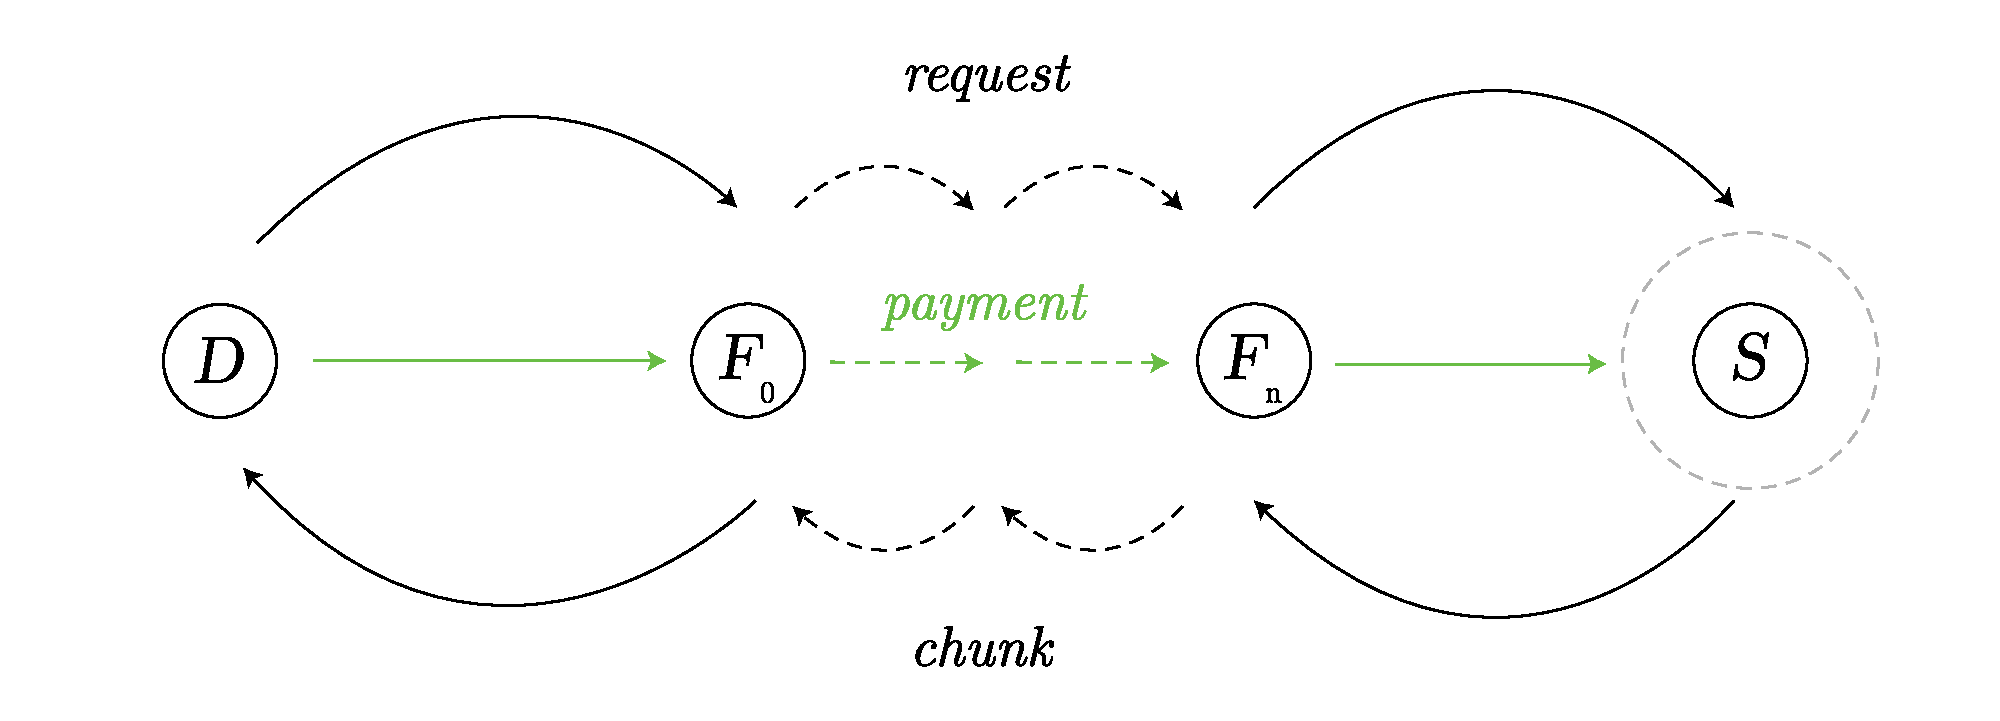
\includegraphics[width=\textwidth]{fig/retrieval-payment.pdf}
   \caption[Incentivising retrieval \statusgreen]{Incentivising retrieval. Node $D$ (Downloader) sends a retrieve request to the chunk's address. Retrieval uses forwarding, so the request is relayed via forwarding nodes $F_0$, ..., $F_n$ all the way to node $S$, the storer node closest to the chunk address. The chunk is delivered by being passed back along the same route to the downloader. Receiving the chunk response triggers an accounting event.}
   \label{fig:retrieval-payment}
\end{figure}

If, however, there is no cost to a request, then sending many illegitimate requests for non-existing chunks (random addresses) becomes possible. This is easily mitigated by imposing sanctions on peers that send too many requests for chunks that do not exist (see \ref{sec:sanctions}).

Once a node initiates (starts or forwards) a request, it commits to pay for that chunk if it is delivered within the defined \gloss{time to live} (\gloss{TTL}), therefore there is never an incentive to block timely deliveries when the chunk is passed back.  This commitment also dissuades nodes from frivolously asking too many peers for a chunk, since, if multiple peers respond with delivery, each must be paid.


\subsection{Pricing protocol for chunk retrieval\statusgreen}\label{sec:pricing}

\green{}

Next, we describe the protocol which nodes use to communicate their price for delivering chunks in the Swarm network. Building on top of this protocol, strategies can then be implemented by nodes who wish to compete in the market with other nodes in terms of quality of service and price. 

\subsubsection{Price discovery}\label{sec:retrieval-price-discovery}

The main merit of the protocol is that it allows for the mechanisms of price discovery to be based only on local decisions, which is essential for the following reasons: (1) Bandwidth costs are not homogeneous around the world: Allowing nodes to express their cost structure via their price will enable competition on price and quality, ultimately benefiting the end-user. (2) The demand for bandwidth resource is constantly changing due to fluctuations in usage or connectivity. (3) Being able to react directly to changes creates a self-regulating system. 

Practically, without this possibility, a node operator might decide to shut down their node when costs go up or, conversely, end-users might overpay for an extended period of time when costs or demand decrease and there is no competitive pressure for nodes to reduce their price accordingly. 

Bandwidth is a service that comes with "instant gratification" and therefore immediate acknowledgement and accounting of its cost are justified. Since it is hard to conceive of any externalities or non-linearities in the overall demand and supply of bandwidth, a pricing mechanism which provides for both (1) efficient and immediate signalling and (2) competitive choice with minimal switching and discovery costs is most likely to accommodate strategies that result in a globally optimal resource allocation.

To facilitate this, we introduce a protocol message that can communicate these prices to upstream peers. We can conceptualise this message as an alternative response to a request. Nodes maintain the prices associated with each peer for each proximity order. Therefore, when they issue a retrieve request, they already know the price they commit to pay as long as the downstream peer successfully delivers the valid chunk within the time-to-live period. However, there is no point in restricting the price signal just to responses: If, for whatever reason, a peer decides to change the prices, it is in the interest of both parties to exchange this information even if there is a request to respond to. In order to prevent DoS attacks by flooding upstream peers with price change messages, the rate of price messages is limited. Well-behaved and competitively priced nodes are favoured by their peers; if a node's prices are set too high or their prices exhibit a much higher volatility than others in the network, then peers will be less willing to request chunks from them.%
%
\footnote{While this suggests that unreasonable pricing is taken care of by market forces, in order to prevent catastrophic connectivity changes as a result of radical price fluctuations, limiting the rate of change may need to be enforced on the protocol level. }

For simplicity of reasoning, we posit that the default price is zero, corresponding to a free service (altruistic strategy). 

\subsubsection{Differential pricing of proximities}\label{sec:diff-pricing-prox}

If the price of a chunk is the same at all proximities, then there is no real incentive for nodes to forward requests other than the potential to cache the chunk and earn revenue by reselling it. This option is hard to justify for new chunks, especially if they are in the shallow proximity orders of a node where they are unlikely to be requested. More importantly, if the pricing of chunks is uniform across proximity orders, colluding nodes can generate chunk traffic and pocket exactly as much as they send, virtually a free DoS attack (see Figure \ref{fig:ddos-uniform-price}).

\begin{figure}[htbp]
   \centering
   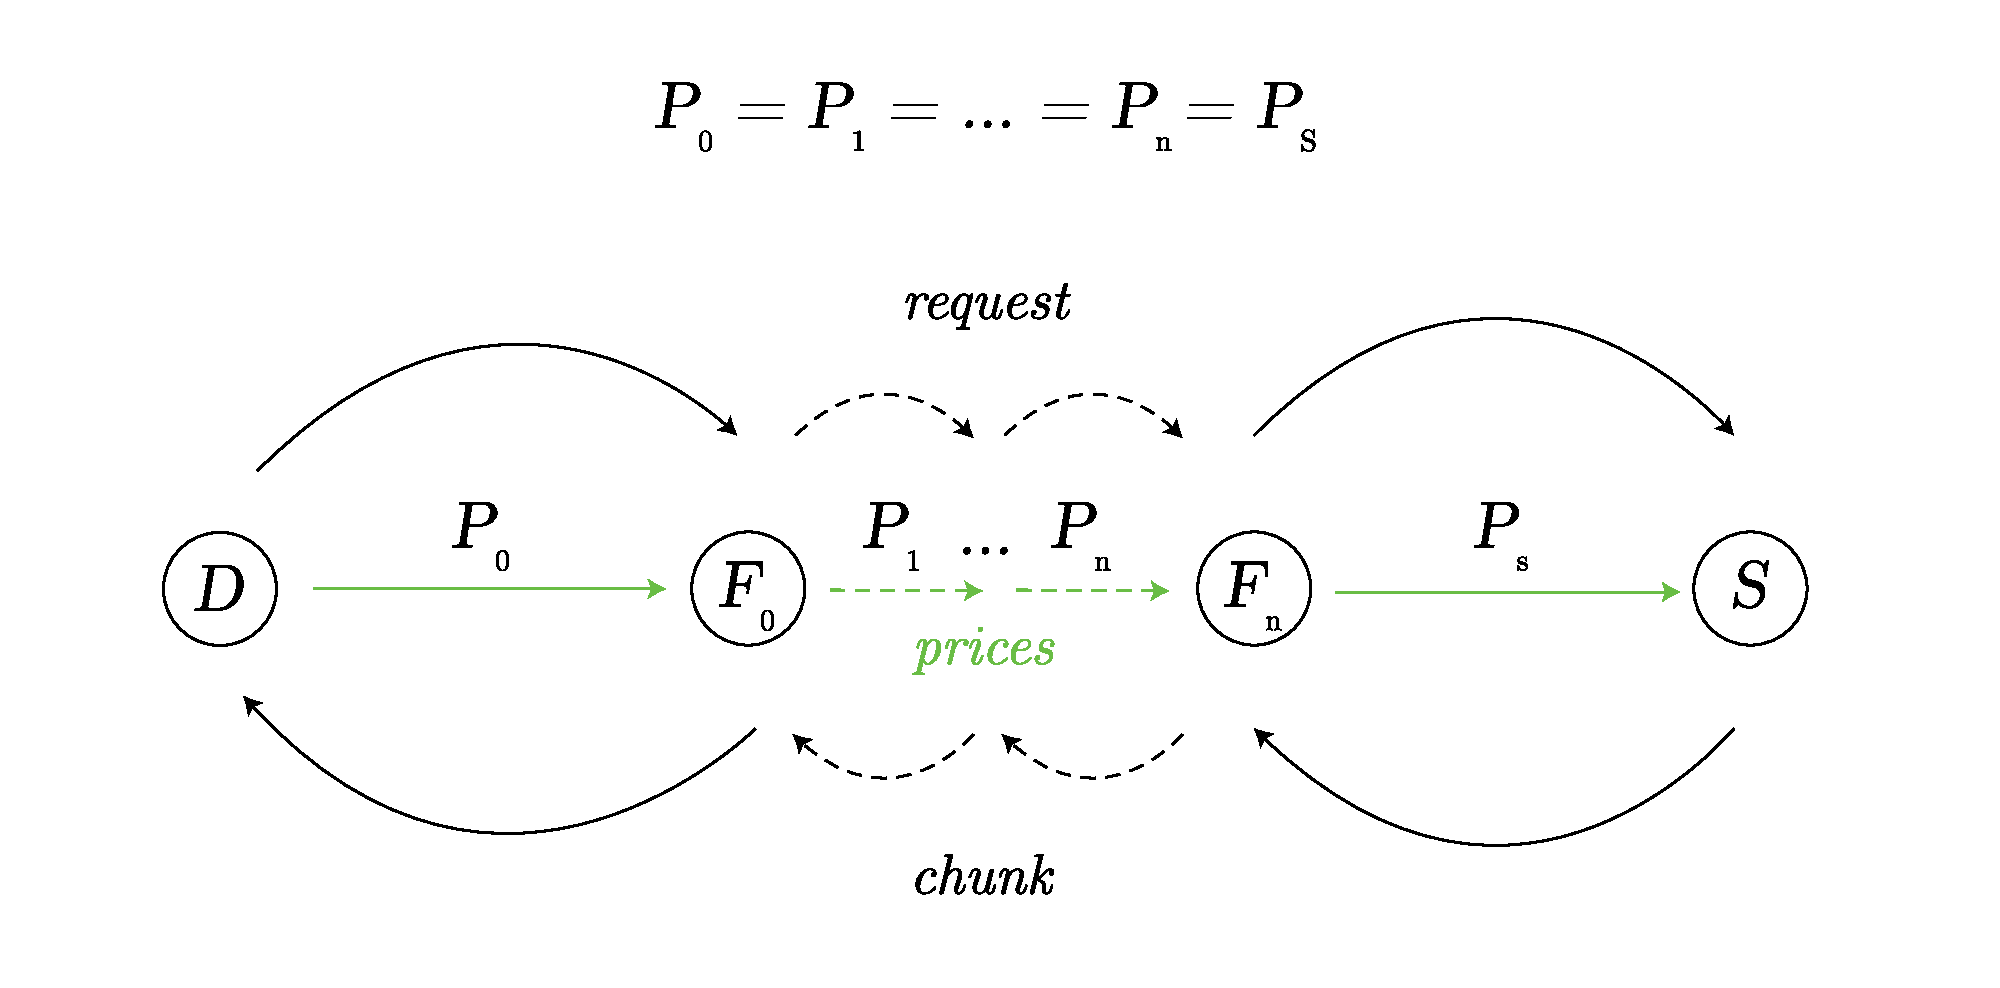
\includegraphics[width=\textwidth]{fig/ddos-uniform-price.pdf}
   \caption[Uniform chunk price across proximities would allow a DoS \statusgreen]{Uniform chunk price across proximities would allow a DoS attack. An attacker can create a flow of traffic between two nodes $D$ and $S$ by sending retrieve requests towards $S$ which only $S$ can serve. If prices are the same across proximities, such an attack would incur no cost for the attacker.}
   \label{fig:ddos-uniform-price}
\end{figure}

To mitigate this attack, the price a requestor pays for a chunk needs to be strictly greater than what the storer node would receive as compensation when a request is routed from requestor to storer. We need to establish a pricing scheme that rewards forwarding nodes, hence, this necessitates the implementation of differential pricing based on node proximity. If the price of delivery is lower as a node gets further from the chunk, then the request can always be sent that way because the forwarder will pocket the difference and therefore make a profit. This means that an effective differential scheme will converge to a pricing model where delivery costs more if the peer is further from the chunk address, i.e. rewards for chunk deliveries are a decreasing function of proximity. 

Due to competitive pressure along the delivery path and in the neighborhood, we expect that the differential a node is applying to the downstream price to converge towards the marginal cost of an instance of forwarding.
The downstream price is determined by the bin density of the node. Assuming balanced bins with cardinality $2^n$, a node can guarantee to increase the proximity order by $n$ in one hop. At the same time, it also means that they can spread the cost over $n$ proximity bins pushing the overall price down.


\subsubsection{Uniformity of price across peers}

Take a node $A$ that needs to forward a request for a chunk which falls into $A$'s PO bin $n$. Notice that all other peers of $A$ in bins $n+1, n+2, ...$, just like $A$ also have the chunk in their PO $n$. If any of these peers, say $B$, has a price  for proximity order $n$ cheaper than $A$, $A$ can lower its price for PO bin $n$, forward all increased traffic to $B$ and still pocket the difference, see Figure  \ref{fig:price-arbitrage}. Note that this is not ideal for the network as it introduces a \gloss{spurious hop} in routing, i.e., in relaying without increasing the proximity. 


\begin{figure}[htbp]
   \centering
   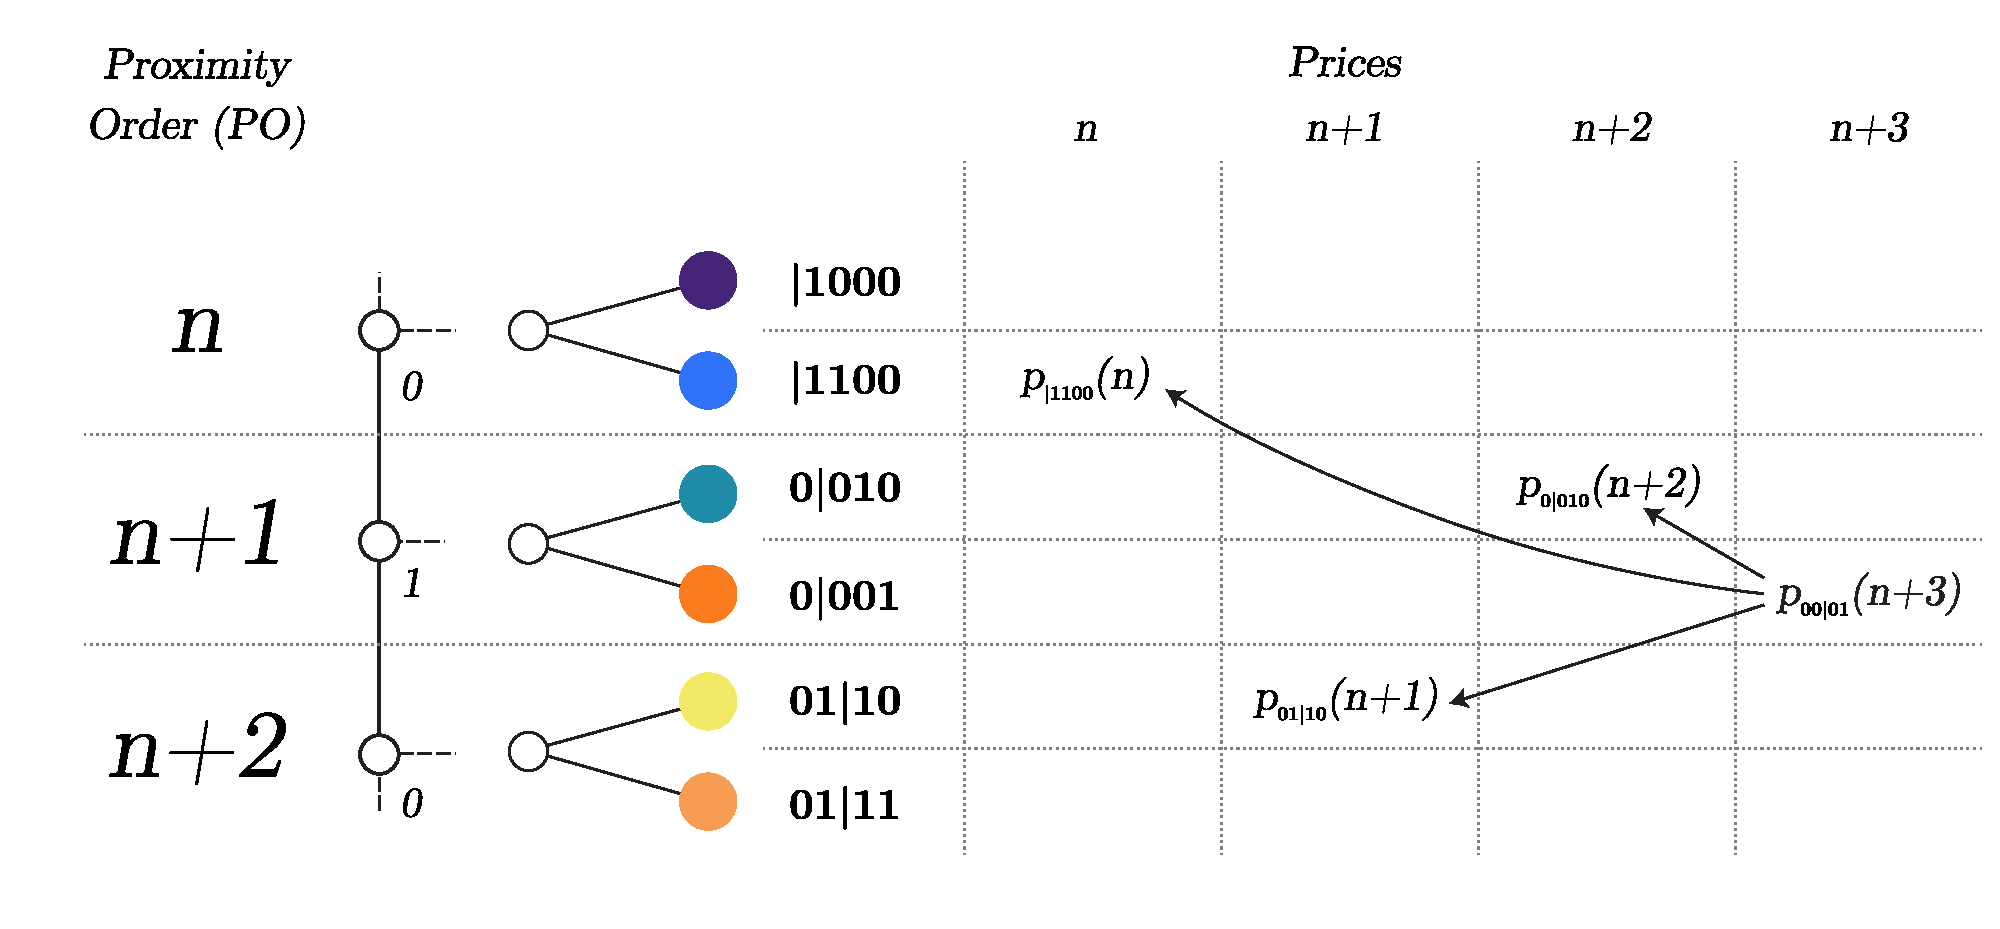
\includegraphics[width=\textwidth]{fig/price-arbitrage-3.pdf}
    \caption[Price arbitrage \statusgreen]{Price arbitrage. Nodes keep a price table for prices of every proximity order for each peer. The diagram shows node $0101$ trying to forward a retrieve request for $0000$. The arrows originate from the closest node, and point to cells where other peers although further from the chunk, offer cheaper to forward. Choosing the cheaper peer will direct traffic away from the overpriced peer and lead to a pressure on both to adjust.}
   \label{fig:price-arbitrage}
\end{figure}
 


Similarly, peers of $A$ in shallower bins that have lower price than $A$ for their respective bins, e.g., $B$ in bin $n-1$ being cheaper than $A$ in bin $n$, then $A$ can always forward any request to $B$ and pocket the difference.

Now let's assume that all peers have price tables which are monotonically decreasing as PO decreases. Also assume that shallower bins have higher prices for bins less than $n$, and all deeper peers in bins higher than $n$ have the same prices for $n$. Let $B$, $C$, $D$ and $E$ be the peers in bin $n$ densely balanced. $A$ wants to  forward a chunk to a peer so that the PO with its target address increases by 3. If peers $B$ and $C$ attempt to collude against $A$ and raise the price of forwarding chunks to bin $n+3$, they are still bound by $D$ and $E$'s price on PO bin $n+2$. In particular, if they are lower than $B$ and $C$ for $n+3$.

Such price discrepancies offer nodes an arbitrage opportunity; the strategy to forward to the cheapest peer will direct traffic away from expensive peers and increase traffic for cheaper ones. As a consequence, prices will adjust. 

All else being equal, this price arbitrage strategy will achieve (1) uniform prices for the same proximity order across the network, (2) prices that linearly decrease as a function of proximity (3) nodes can increase connectivity and keep prices lower. In this way, incentivisation is designed so that strategies that are beneficial to individual nodes are also neatly aligned in order to benefit the health of the system as a whole.


\subsubsection{Bin density}

Charging based on the downstream peer's proximity to the chunk has the important consequence that the net revenue earned from a single act of non-local delivery to a single requestor is a monotonically increasing function of the difference between the chunk's proximity to the node itself and to the peer the request was forwarded to. In other words, the more distance we can cover in one forward request, the more we earn. 

This incentive aligns with downloaders' interest to save hops in serving their requests, leading to lower-latency delivery and reduced bandwidth overhead. This scheme incentivises nodes to keep a gap-free balanced set of addresses in their Kademlia bins as deep as possible (see Figure \ref{fig:bindensity}), i.e, it is better for a node to keep dense Kademlia bins than thin ones.


Nodes that are able to maintain denser bins actually have the same cost as thinner ones, but saving hops will improve latency and make the peer more efficient. This will lead to the peer being preferred over other peers that have the same prices. Increased traffic essentially can also lead to bandwidth contention, which eventually allows the raising of prices. 

Note that such arbitrage is more efficient in \glossplural{shallow bin} where the number of peers to choose from is higher. This is in major opposition to \glossplural{deep bin} in the area of responsibility. If a node does not replicate its neighbourhood's chunks, some of these chunks will need to be requested by the node closer to the address, but further from the node. This will only be possible at a loss. An added incentive for neighbours to replicate their area of responsibility is discussed in \ref{sec:redistribution}. With the area of responsibility stored however, a node can choose to set their price arbitrarily. 


\subsubsection{Caching and auto-scaling}\label{sec:caching}

Nodes receive a reward every time they serve a chunk, therefore the profitability of a chunk is proportional to its popularity: the more often a chunk is requested, the higher the reward relative to the fixed cost of storage per time unit. When nodes reach storage capacity limits and need to decide which chunks to delete, a rational agent seeking to maximise profit would opt to remove chunks with the lowest profitability. A reasonably%
%
\footnote{Better metrics for predicting chunk profitability than the age of last request will continue to be identified and developed.}
good predictor for this is the age of last request. In order to maximise the set of chunks to select from, nodes engage in opportunistic caching of the deliveries they relay as well as the chunks they sync. This results in popular chunks being more widely spread and faster served, transforming the whole of Swarm into an auto-scaled and auto-balanced \emph{content distribution network}.


\subsubsection{Non-caching nodes}

Any scheme that ensures \glossplural{relaying node} make a profit creates a positive incentive for forwarding-only non-caching nodes to enter the network. Such nodes are not inherently beneficial to the network as they are creating unnecessary bandwidth overhead. On the one hand, their presence could, in principle, unburden storer nodes from relaying traffic, so using them in shallow bins may not be detrimental. On the other hand, closer to neighbourhood depth, their peers will favour a caching/storing node to them because of their disadvantage at least for chunks in their hypothetical area of responsibility. Non-caching nodes can also contribute to increase anonymity (see \ref{sec:retrieval}).

\subsection{Incentivising push-syncing\statusgreen}\label{sec:push-sync-incentives}

\green{}

The push-sync (see \ref{sec:push-syncing}) protocol ensures that chunks uploaded into the network arrive at their designated address. In what follows, we will explain how forwarding is incentivised.
%
%
\footnote{To complement our solution for bandwidth compensation, further measures are needed for spam protection and storage incentivisation which are discussed later in \ref{sec:postage-stamps} and \ref{sec:redistribution}, respectively.}



Push-syncing is analogous to the retrieval protocol in the sense that their respective message exchange sequences travel the same route.
The delivery of the chunk in the push-sync protocol is analogous to a retrieval request and, conversely, the statement of custody receipt in push-sync is analogous to the chunk delivery response in retrieval.

In principle, push-syncing could be left without explicit forwarding incentives. Due to the retrieval protocol, as nodes expect chunks to be found in the neighbourhood of their address, participants in Swarm are at least weakly incentivised to help deliver uploaded chunks to their destination. However, we  need to provide the possibility that chunks are uploaded via nodes further from it than the requestor (light  nodes or retries). Thus, if push-syncing was free, nodes could generate wasteful amounts of bandwidth. 

Requiring payment only for push-sync delivery by downstream peers would put the forwarder in a position to bargain with a storer node regarding the delivery of the chunk. The possession of a chunk is valuable for the prospective storer node because there is also a system of rewards for storage (see \ref{sec:redistribution}). Based on this, the forwarder node could, in theory, hold onto the chunk unless the storer node pays marginally more than the value of possessing that chunk, factoring in the profit potential due to storage incentives. In particular, since forwarders on the route from the uploader are not numerous, any profits generated from a storage reward mechanism might be captured by these forwarding nodes.

Instead, in push-sync, by making the statement of custody receipt a paid message, the roles switch. The forwarder node is no longer in the position to bargain. To understand why, let's consider a scenario where a forwarding node tries to hold on to a chunk to negotiate a price for pushing it to a storer node. In this case, the uploader will not get a statement of custody receipt within the expected time frame. As a result, the uploader will assume that the attempt has failed and re-upload the chunk via a different route. Now, suddenly the original forwarding node is forced to compete with another forwarding node in getting compensation for their bandwidth costs. Since all forwarding nodes are aware of this dynamic, emergent behavior will produce a series of peers that are willing to forward the chunk to the storer node for a relatively small compensation and the bandwidth costs incurred. This eliminates the need for the original forwarding node to try and bargain with the storer node in the first place: Instead, they can generate a small profit immediately by simply returning the statement of custody receipt. 


\begin{figure}[htbp]
\centering
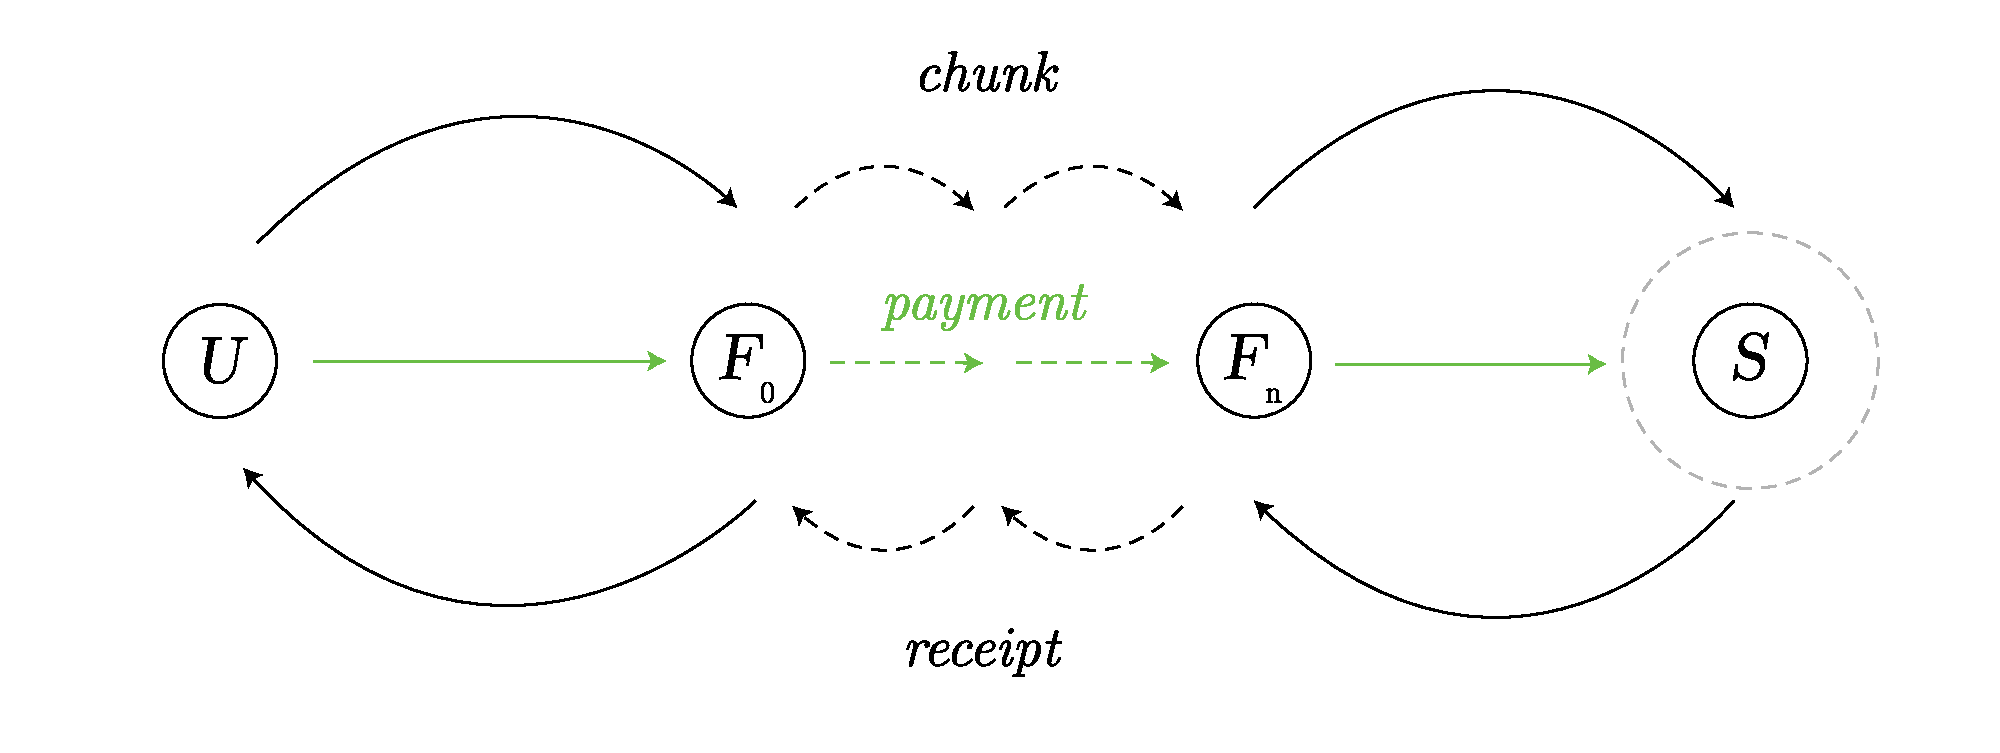
\includegraphics[width=\textwidth]{fig/push-payment.pdf}
\caption[Incentives for push-sync protocol \statusgreen]{Incentives for push-sync protocol. Node $U$ (uploader) sends the chunk towards its address, the closest node to which is node $S$ (storer) via forwarding nodes $F_0, \ldots F_n$. The storer node responds with a statement of custody receipt which is passed back to the uploader via the same forwarding nodes $F_n, \ldots F_0$. Receiving the statement of custody receipt triggers an accounting event.}
\label{fig:syncing-swap}
\end{figure}

This scheme highlights why the incentivisation of the two protocols relies on the same premises: there are many sellers (forwarders) and only one buyer (uploader) for a homogeneous good (the statement of custody receipt). As a result, the price of the service (delivering the chunk to the storer) is determined by the sum of the marginal costs of forwarding for each node along the route. At the same time, the storer node can capture all the profits from the storage compensation scheme.

In this way, we can make sure that (1) storers actually respond with receipts, and (2) have a way to detect timed out or unsolicited receipt responses to protect against DoS, see Figure \ref{fig:syncing-swap}.

Similar to the retrieval protocol, the pricing in this scheme is expected to vary based on different proximities (see \ref{sec:diff-pricing-prox}). Additionally, as the costs of the nodes in the network fluctuate (depending on capacity utilization and node efficiency), the pricing will also be subject to change over time. Given that the compensation is calculated for one chunk and one shorter message (retrieve request and custody receipt) during the accounting process, we can safely conclude that the price structure for forwarding for both protocols is identical. Consequently, a unified pricing scheme for forwarding can be applied to both protocols, as discussed in \ref{sec:retrieval-price-discovery}. 
What distinguishes push-sync from the retrieval protocol is that, unlike in retrieval where the chunk is delivered back and its integrity can be validated, the accounting event in push-sync is a statement of custody which can be spoofed. Due to the forwarding incentive, nodes may be motivated to withhold forwarding and impersonate a storer node by issuing the statement of  custody. This makes it advisable to query (retrieve) a chunk via alternative routes. If  such  retrieval attempts fail, it may be necessary to try push-syncing chunks through alternative routes. 
 

\section{Swap: accounting and settlement\statusgreen}\label{sec:accounting-and-settlement}

\green{}

This section covers aspects of incentivisation relating to bandwidth sharing. 
In \ref{sec:accounting}, we introduce a mechanism to keep track of the data traffic between peers and offer peer-to peer-accounting for message relaying.
Subsequently, in \ref{sec:cheques}, we describe the conditions of compensating for unbalanced services and show how settlement can be achieved.
In particular we introduce the concept of a. \glossplural{cheque} and the \gloss{chequebook contract}. In \ref{sec:waiver}, we discuss waivers as an optimisation that allows for additional savings on transaction costs. In \ref{sec:zero-cash-entry} we discuss how an incentivised service of sending in cashing transactions enables zero-cash entry to Swarm and, finally, in \ref{sec:sanctions} we delve into the fundamental set of sanctions that serve as incentives for nodes to play nice and adhere to the protocols.

\subsection{Peer to peer accounting\statusgreen}\label{sec:accounting}


\cite{ethersphere2016sw3} introduces a protocol for peer-to-peer accounting, called \gloss{swap}. Swap is a tit-for-tat accounting scheme that scales microtransactions. The scheme allows directly connected peers to swap payments or payment commitments. The system's key characteristics are captured playfully with different mnemonic resolutions of the acronym SWAP:

\begin{itemize}[noitemsep]
    \item \emph{Swarm accounting protocol} for \emph{service wanted and provided} -- An account service for service exchange.
    \item \emph{settle with automated payments} -- Send a \gloss{cheque} when \gloss{payment threshold} is exceeded.
    \item \emph{send waiver as payment} -- Debt can be waived in the value of un-cashed cheques. 
    \item \emph{start without a penny} and \emph{send with a peer} -- Zero-cash entry is supported by unidirectional swap.
\end{itemize}

\subsubsection{Service for service}

\gloss{swap} allows service for service exchange between connected peers. When there is equal consumption with low variance over time, bidirectional services can be accounted for without the need for any payments. Data relaying is an example of such a service, making Swap well-suited for implementing bandwidth incentives in content delivery or mesh networks.

\begin{figure}[htbp]

\begin{center}
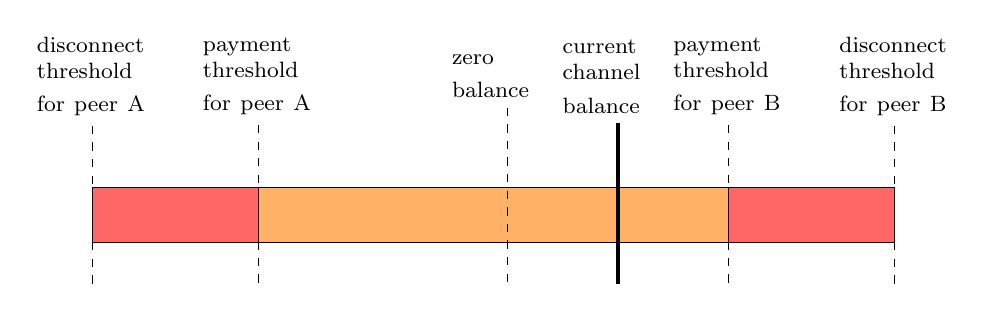
\begin{tikzpicture}
\node (middle)[draw, rectangle, fill=orange!60, minimum height=2em, minimum width=18em]{};
\node (leftred) [draw, rectangle, fill=red!60, minimum height=2em, minimum width=6em, node distance=12em,left of=middle]{};
\node (rightred)[draw, rectangle, fill=red!60, minimum height=2em, minimum width=6em, node distance=11em,right of=middle]{};
\node (zero) [above of=middle,node distance=5em, text width=4em, align=left] {\footnotesize zero\\ balance};
\node (zerod) [below of=middle] {};
\draw [dashed](zero)--(zerod);
\node (rtol) [node distance=8em,right of=zero,text width=4em, align=left] {\footnotesize payment\\threshold\\for peer B};
\node (rtold) [node distance=8em,right of=zerod] {};
\node (ltol) [node distance=9em,left of=zero,text width=4em, align=left] {\footnotesize payment\\threshold\\for peer A};
\node (ltold) [node distance=9em,left of=zerod] {};
\node (rdis) [node distance=14em, right of=zero,text width=4em, align=left] {\footnotesize disconnect\\threshold\\for peer B};
\node (rdisd) [node distance=14em,right of=zerod] {};
\node (ldis) [node distance=15em, left of=zero,text width=4em, align=left] {\footnotesize disconnect\\threshold\\for peer A};
\node (ldisd) [node distance=15em,left of=zerod] {};
\node (rbal) [node distance=4em,right of=zero,text width=4em, align=left] {\footnotesize current\\channel\\balance};
\node (rbald) [node distance=4em,right of=zerod] {};

\draw [dashed](rtol)--(rtold);
\draw [dashed](ltol)--(ltold);
\draw [dashed](rdis)--(rdisd);
\draw [dashed](ldis)--(ldisd);
\draw [very thick](rbal)--(rbald);
\end{tikzpicture}
\end{center}
\caption[Swap balance and swap thresholds \statusgreen]{Swap balance and swap thresholds.
Zero balance in the middle indicates the equal consumption and provision of services.
The current channel balance represents the difference in uncompensated service provision:
If the balance is to the right of zero, it tilts in favour of A with peer B being in debt, whereas to the left,
the balance tilts in favour of B with A being in debt.
The orange interval represents loss tolerance. When the balance exceeds the payment threshold, the party in
debt sends a \gloss{cheque} to its peer. If it reaches the \gloss{disconnect threshold}, the peer in debt is disconnected.}
\label{fig:swap}
\end{figure}

\subsubsection{Settling with payments}

In situations where there is high variance or unequal consumption of services, the balance will eventually tilt significantly toward one peer. In such cases, the indebted party issues a payment to the creditor to restore the nominal balance to zero. This process is automatic and justifies the concept of swap as \emph{settle (the balance) with automated payments} (see Figure \ref{fig:swap}). These payments can be in the form of commitments rather than immediate transactions.


\subsubsection{Payment thresholds}

To quantify what counts as "significant tilt", the swap protocol requires peers to advertise a \gloss{payment threshold} as part of the handshake: When their relative debt to their peer goes above this threshold, they send a message containing a payment to their peer. It is reasonable for any node to send a message when the debt reaches this level, as there is also a disconnect threshold in place. The disconnect threshold can be set freely by any peer, but it is recommended to choose a value that takes into account the usual 
variance in accounting balances between the two peers. This can be done by considering the difference between the payment threshold and the disconnect threshold.


\subsubsection{Atomicity}

Sending the \gloss{cheque} and updating the balance on the receiving side cannot be made an atomic operation without substantial added complexity. For instance, a client could crash between receiving and processing the message, so even if the sending returns with no error, the sending peer can not be sure the payment was received, this can result in discrepancies in accounting on both sides. The tolerance expressed by the difference between the two thresholds ($\mathit{DisconnectThreshold}-\mathit{PaymentThreshold}$) guards against this, i.e. if the occurrence of such crashes is infrequent and happens with roughly equal probability for both peers, the resulting minor discrepancies are filtered out. This mechanism protects nodes from facing sanctions.

\begin{center}
\begin{figure}[htbp]
\input{fig/chequeswap.tex}
\caption[Cheque swap \statusgreen]{Peer B's swap balance (with respect to A) reaches the payment threshold (left),
B sends a cheque to peer A. B keeps the cheque and restores the swap balance to zero.}
\label{fig:chequeswap}
\end{figure}
\end{center}

\subsection{Cheques as off-chain commitments to pay\statusgreen}\label{sec:cheques}

One of the major challenges with conducting direct \glossplural{on-chain payment} in a blockchain network is the high transaction costs associated with processing each transaction by every participating node. It is, however, possible to create a payment without presenting this payment on-chain. Such payments are called \gloss{second-layer payment} strategies. One such strategy is deferring payments and processing them in bulk. In exchange for reduced cost, the beneficiary must be willing to incur a higher risk of settlement failure. We argue that this is perfectly acceptable in the case of bandwidth incentivisation in Swarm, where peers will engage in repeated dealings.


\subsubsection{The chequebook contract}

A simple smart contract called the \gloss{chequebook contract}, introduced in \cite{ethersphere2016sw3}, allows the beneficiary to determine the timing of payments. This contract acts as a wallet that can process \glossplural{cheque} issued by its owner. Similar to traditional financial transactions, the issuer signs a \emph{cheque} specifying the \emph{beneficiary}, \emph{date}, and \emph{amount}, providing it to the recipient as a token of promise to pay at a later date. The smart contract plays the role of the bank. When the recipient wishes to get paid, they "cash the cheque" by submitting it to the smart contract. The contract, after validating the signature, date and the amount specified on the cheque, transfers the amount to the beneficiary's account (see Figure \ref{fig:swap-chequebook}). Analogous to the person taking the cheque to the bank to cash it, anyone can send a digital cheque in a transaction to the owner's chequebook account, initiating the transfer. 

The swap protocol specifies that when the \emph{payment threshold} is exceeded, a cheque is sent over by the creditor peer. Such cheques can be immediately cashed by sending them to the issuer's chequebook contract. Alternatively, cheques can also be held, which effectively serves as a form of lending on credit, enabling parties to save on transaction costs. 

The amount deposited in the chequebook (\gloss{global balance}) serves as collateral for the cheques and is pooled over the beneficiaries of all outstanding cheques. In this simplest form, the chequebook provides the same guarantees as real-world cheques: None. Since funds can be freely moved out of the chequebook wallet at any time, solvency at the time of cashing can never be guaranteed: If the chequebook's balance is less than the amount specified in a submitted cheque, the cheque will bounce. This is the trade-off between transaction costs and risk of settlement failure.

While, strictly speaking, there are no guarantees for solvency, nor is there an explicit punitive measure in the case of insolvency, a bounced cheque can negatively impact the issuer's reputation as the chequebook contract records such incidents. On the premise that cheques are swapped in the context of repeating dealings, peers will refrain from issuing cheques beyond their balance. In other words, a node's interest in keeping a good reputation with their peers serves as a sufficient incentive to maintain its solvency.


\begin{figure}[htbp]
\centering
\input{fig/swap.tex}
\caption[The basic interaction sequence for swap chequebooks \statusgreen]{The basic interaction sequence for swap chequebooks}
\label{fig:swap-chequebook}
\end{figure}


\subsubsection{Double cashing}

Since these digital cheques are files and can therefore be copied, it is crucial to implement measures to prevent the cashing of the same cheque multiple times. Such "double cashing" can be prevented by assigning each cheque given to a particular beneficiary a serial number which the contract will store when the cheque is cashed. The chequebook contract can then rely on the serial number to make sure cheques are cashed in sequential order, thus needing to store only a single serial number per beneficiary.

Alternatively, to address repeated payments to the same beneficiary, the cheques can contain the \emph{cumulative} total amount ever credited to that beneficiary. The contract maintains a record of the total amount that has been cashed out for each beneficiary, and when a new cheque is submitted, the contract compares the amount on the cheque to the stored total. Cheques with an amount equal to or less than the stored total are ignored, while cheques with a higher total will result in the transfer of the difference to the beneficiary.


This simple trick also makes it possible to cash cheques in bulk because only the most recent "last cheque" needs to be processed, leading to a significant reduction of transaction costs.

\subsubsection{Cashing without Ether}\label{sec:zero_eth}
Not all peers in Swarm are expected to have the Ether needed to pay for the transaction costs to cash out a cheque. The chequebook allows third parties to cash cheques. The sender of the transaction is incentivised with a reward for the service performed.

\subsection{Waivers\statusgreen}\label{sec:waiver}

If the imbalance in the swap channel is due to high variance rather than unequal consumption, after a period of accumulating cheques, the channel balance starts tilting in the opposite direction. Normally, it is now up to the other party to issue cheques to its peer, resulting in uncashed cheques accumulating on both sides.
To allow for further savings in transaction costs, it might be desirable to be able to offset these cheques against each other.

Such a process is possible, but it requires certain important changes within the chequebook contract. In particular, cashing cheques can no longer be immediate and must incur a security delay, a concept familiar from other payment channel implementations \cite{poon2015bitcoin, diferrante2017payment, mcdonald2017payment, tremback2015universal}. 

Let us imagine a system analogous to cheques being returned to the issuer. Assume peer $A$ issued cheques to $B$ and the balance was brought back to zero. Later, the balance tilts in $A$'s favour, but the cheques from $A$ to $B$ have not been cashed. In the traditional financial world, $B$ could either simply return the last cheque to $A$ or provably destroy it. In our case, it is not so simple; we need some other mechanism by which $B$ \emph{commits not to cash} that particular cheque. Such a commitment could take several forms; it could be implemented by $B$ signing a message allowing $A$ to issue a new `last cheque` with a lower cumulative total amount than before, or perhaps $B$ could issue a form of `negative` cheque for A's chequebook, effectively offsetting the amount as if a cheque with the same amount had been paid. 

These implementations share the characteristics of not allowing the instantaneous cashing of cheques in the chequebook. Upon receiving a cheque-cashing request, the contract must wait to allow the other party to submit potentially missing information about cancelled cheques or reduced totals. To accommodate (semi-)bidirectional payments using a single chequebook, we introduce the following modifications:

\begin{enumerate}[noitemsep]
    \item All cheques from user A to user B must contain a serial number.
    \item Each new cheque issued by A to B must have a serial number higher than the previous one.
    \item A's chequebook contract records the serial number of the last cheque that B cashed.
    \item During the cashing delay, any valid cheque with a higher serial number supersedes any previously submitted cheques, regardless of their face value.
    \item Any submitted cheque which decreases the payout of the previously submitted cheque is only valid if it is signed by the beneficiary.
\end{enumerate}


\begin{figure}[htbp]
\centering
\includegraphics[width=\textwidth]{fig/waivers-diagram-2.pdf}
\caption[Example sequence of mixed cheques and waivers exchange \statusgreen]{Example sequence of mixed cheques and waivers exchange}
\label{fig:waivers-diagram}
\end{figure}

With these rules in place, it is easy to see how cheque cancellation would work. Let's consider the scenario where user $A$ has issued cheques $c_0 \ldots c_n$ with cumulative totals $t_0 \ldots t_n$ to user $B$. Suppose that the last cheque $B$ cashed was $c_i$. The chequebook contract has recorded that $B$ has received a payout of $t_i$ and that the last cheque cashed had serial number $i$.

Let us further suppose that the balance starts tilting in $A$'s favour by some amount $x$. If $B$ had already cashed cheque $c_n$, then $B$ would be required to issue a cheque of her own using $B$'s chequebook as the source and naming $A$ as the beneficiary. However, since cheques $c_{i+1} \ldots c_n$  are still uncashed, $B$ can instead send to $A$ a cheque with $A$'s chequebook as the source, $B$ as the beneficiary, with serial number $n+1$ and cumulative total $t_{n+1} = t_n - x$. Due to the rules enumerated above, $A$ will accept this as an equivalent payment of amount $x$ from $B$.  In this scenario, instead of sending a cheque to $A$, $B$ waives part of their earlier entitlement. This justifies the concept of SWAP as \emph{send waiver as payment}.

This process can be repeated multiple times until the cumulative total is brought back to $t_i$. At this point, all outstanding debt has effectively been cancelled, and any further payments must be made in the form of a proper cheque from $B$'s chequebook to $A$ (see Figure \ref{fig:waivers-diagram}).

% \subsection{Best effort settlement strategy}

% Abels text

\subsection{Zero cash entry\statusgreen}\label{sec:zero-cash-entry}


Swap accounting can also work in a one-directional manner. When a party enters the system with zero liquid capital (a \gloss{newcomer}) but connects to a peer with funds (an \gloss{insider}), the newcomer can begin to provide a service (and not use any) in order to earn a positive swap balance. 

If the insider has a chequebook, they are able to simply pay the newcomer with a cheque. However, this has a caveat: The newcomer will be able to earn cheques for the services provided but will not have the means to cash them. Cashing cheques requires sending a transaction to the blockchain, and therefore requires gas, unless the node can convince one of its peers to execute the transaction on its behalf. To facilitate this, nodes are able to sign off on a structure that they want to be sent, and then extend the Swap contract with a preprocessing step that triggers payment to the newcomer, covering the transaction’s gas cost plus a service fee for the sender of the transaction. The newcomer's cheque may be cashed by any insider (see Figure \ref{fig:zero-cash-entry}). This feature justifies the concept of SWAP as \emph{start without a penny, send with a peer}.

\begin{figure}[htbp]
\centering
\input{fig/zero-cash-entry.tex}
\caption[Zero cash entry \statusorange]{Bootstrapping or how to launch as a swap capable node consuming and providing a
service and earn money.}
\label{fig:zero-cash-entry}
\end{figure}

The possibility to earn small amounts of money without starting capital is crucial, as it provides a way for new users to get access to Swarm without the need to purchase the token. This benefit extends to the Ethereum ecosystem in general: using Swarm, anybody can earn small amounts of money to start paying the gas to fuel their dapps, without the need to go through a painful process of acquiring tokens prior to onboarding. 


% \subsection{Cashing out and risk of insolvency\statusred}



\subsection{Sanctions and blacklisting \statusgreen}\label{sec:sanctions}
\red{}

This section complements the SWAP scheme with additional incentives and protection against foul play. 

\subsubsection{Protocol breach}

In a peer-to-peer trustless setting, implementing nuanced sanctions against undesired peer behaviour can be challenging. However, when the basic rules of interaction are violated, the node that detects it can simply disconnect from that peer. In order to avoid deadlocks due to attempted reconnection, the sanctions imposed on transgressive nodes also include recording the peer's address into a blacklist. This simple measure is enough to provide a clear disincentive to nodes seeking to exploit the protocol. 

\subsubsection{Excessive frivolity}

Both retrieval and push-sync protocols have an incentive structure where only the response to a request generates income. Although this creates a strong incentive to play ball, it may also be necessary to take measures to ensure that nodes are not able to spam the network with frivolous requests that have no associated cost. In the case of push-syncing, it is especially important not to allow chunks to expunge others at no cost. This will form the topic of a later section where we introduce postage stamps (see \ref{sec:postage-stamps}).

In the case of pull-sync retrieval, the potential attack consists of requesting non-existing chunks and causing downstream peers to initiate a lot of network traffic, as well as some memory consumption, due to requests being persisted during the time-to-live period.
Surely, there is a possibility that a requestor may unknowingly request non-existing chunks, and what is more, the requested chunk could have been be garbage-collected in the network, in which case, the requestor may have acted in good faith. 

To mitigate this, each node maintains a record of the number of retrieve requests from each of its peers and then updates the relative frequency of failed requests, i.e. requests that have timed out even though the node in question had forwarded it. If the proportion of failed requests to successful requests exceeds a certain threshold, sanctions are imposed on the peer: it is disconnected and blacklisted.

% 
% \footnote{Note that policing frivolous requestors is much easier than policing forwarders, since the latter requires positive evidence from other nodes while the former only requires forwarding.}
%

By remembering the requests they have forwarded, nodes can distinguish legitimate responses from a potential DoS attack: for retrieval, if the chunk delivered does not fulfil an open request, it is considered unsolicited; for push-sync, if a statement of custody response does not match an existing entry for forwarded chunk, it is considered unsolicited.

Timeouts are crucial here. After the time-to-live period for a request has passed, the record of the open request can be removed. Any response received after this point is considered unsolicited, as it is indistinguishable from messages that were never requested. 

To account for slight discrepancies in time measurement, once again a small percentage of illegitimate messages are tolerated from a peer before they are disconnected and blacklisted.

\subsubsection{Quality of service}

Beyond the rate of unsolicited messages, nodes can cause grievances on other ways, such as by setting high prices, having low network throughput, or long response latencies. Similarly to excessively frivolous requests, there is no need for a distinction between malicious attacks or sub-optimal (poor quality, overpriced) service provided in good faith. As a result, mitigating quality of service issues is discussed in the context of peer selection strategies in forwarding and connectivity.

\subsubsection{Blacklisting}

Blacklisting is a strategy that complements disconnection as a measure against peers. It is supposed to extend our judgment expressed in the act of disconnection that the peer is unfit for business.
Blacklists serve as a reference when accepting incoming connections as well as in the peer suggestion strategy of the connectivity driver. On the one hand, blacklisting can save the node from being deadlocked in a cycle of malicious peers trying to reconnect. On the other hand, care must be taken not to blacklist peers acting in good faith, as this could negatively impact network connectivity.


\section{Postage stamps}\label{sec:postage-stamps}

A postage stamp is a verifiable proof of payment associated with a chunk witnessed by the signature of its owner. On the one hand, postage stamps prevent frivolous uploads by imposing an advance cost. On the other hand, by ascribing a quantity of BZZ, they signal a chunk's relative importance which storer nodes can then use to rank chunks when selecting which ones to retain and serve, and which ones to garbage collect in the event of capacity shortage.

In this section we first introduce the concept of postage batch enabling the bulk purchase of stamps (\ref{sec:purchasing-upload}). In \ref{sec:limited-issuance}, we explain how limited issuance is represented and enforced. In \ref{sec:reserve}, we introduce the notion of reserve and detail the rules governing how storer nodes keep it maximally utilised. We conclude in \ref{sec:depths} with exploring the relationship between reserved capacity, effective demand and the number of nodes and their impact on the data availability.

\subsection{Purchasing upload capacity}\label{sec:purchasing-upload}

% \subsubsection{Postage batches and the postage smart contract}

Uploaders purchase postage stamps in bulk in the form of a \gloss{postage batch} from the postage smart contract on the Ethereum blockchain. Postage batches are created by this contract when a transaction is sent to its batch creation endpoint, together with an amount of BZZ tokens and transaction data specifying some parameters. As the transaction executes, a new batch entry is registered in the postage contract with the following pieces of information:

\begin{itemize}[noitemsep]
\item[--] \emph{batch identifier} -- A random ID that is generated to provide reference for this batch.
\item[--] \emph{batch depth} -- Base 2 logarithm of the \gloss{issuance volume}, i.e., number of chunks that can be stamped using this batch. 
\item[--] \emph{owner address} -- The Ethereum address of the owner entitled to issue stamps, as per the transaction data sent along with the creation or the  transaction sender if not specified.
\item[--] \emph{per-chunk balance} -- The total amount sent along with the transaction divided by the issuance volume.
\item[--] \emph{mutability} -- A boolean flag indicating if the storage slots of the batch can be reassigned to another chunk with a stamp if its timestamp is older. 
\item[--] \emph{uniformity depth} -- the base 2 logarithm of the number of equal-size buckets the storage slots are arranged in.
\end{itemize}

The postage contract provides endpoints to users to modify the per-chunk balance of batches, i.e., add funds to extend the validity period of the stamps issued by the batch (\/\emph{top-up}) or add volume to decrease it (\/\emph{dilute}).
Anyone can then choose to top up the balance of a batch at a later date but only the owner can dilute it.%
%
\footnote{As a planned feature, the remaining balance of a batch can be reassigned to a new batch, resulting in the immediate expiry of the original.}


% \subsubsection{Stamp validity}

\begin{figure}[!ht]
  \centering
    
\includegraphics[width=\textwidth]{fig/postage-stamp-structure.pdf}
  \caption[Postage stamp]{Postage stamp is a data structure comprised of the postage contract batch id, storage slot index, timestamp the chunk address and a witness signature attesting to the association of these four. Uploaders and forwarders must attach a valid postage stamp to every chunk uploaded. }
  \label{fig:postage-stamp}
\end{figure}

Owners issue postage stamps in order to attach them to chunks%
% (see definition \ref{def:postage-stamp} in appendix \ref{sec:appendix-disc})%
. A batch has a number of \glossplural{storage slot} effectively arranged over a number of equal sized buckets. Issuing a stamp means to assign a chunk to a storage slot. A stamp is a data structure comprising the following fields (see figure  \ref{fig:postage-stamp}):

\begin{itemize}[noitemsep]
    \item[--] \emph{chunk address} -- The address of the chunk the stamp is attached to. 
    \item[--] \emph{batch identifier} --  The ID referencing the issuing batch (generated at its creation).
    \item[--] \emph{storage slot} -- An bucket index referencing one of the equal sized buckets of the batch and a within-bucket index referencing the storage slot the chunk is assigned to.
    \item[--] \emph{timestamp} -- The time the chunk is stamped. 
    \item[--] \emph{witness} -- The batch owner's signature attesting to link between the storage slot and the chunk.
\end{itemize}

A postage stamp's validity can be checked by verifying that it scores all true on the following five attributes%
% (see definition \ref{def:postage-stamp-validity} in appendix \ref{sec:appendix-disc})%
:

\begin{itemize}[noitemsep]
\item[--] \emph{authentic} -- The batch identifier is registered in the postage contract's storage.
\item[--] \emph{alive} -- The referenced batch has not yet exhausted its balance.
\item[--] \emph{authorised} -- The postage stamp is signed by the address specified as the owner of the batch. 
\item[--] \emph{available} -- The referenced storage slot is within range given the batch depth, and, in the case of an immutable batch, has no duplicates.
\item[--] \emph{aligned} -- The referenced storage slot has the bucket specified and it aligns with the chunk address stamped.
\end{itemize}

All this can be easily checked by nodes in the swarm only using information available on the public blockchain (read-only endpoints of the postage contract). When a chunk is uploaded, the validity of attached postage stamp is verified by forwarders along the push-syncing route  (see figure \ref{fig:postage-stamps}).


\begin{figure}[!th]
\centering
  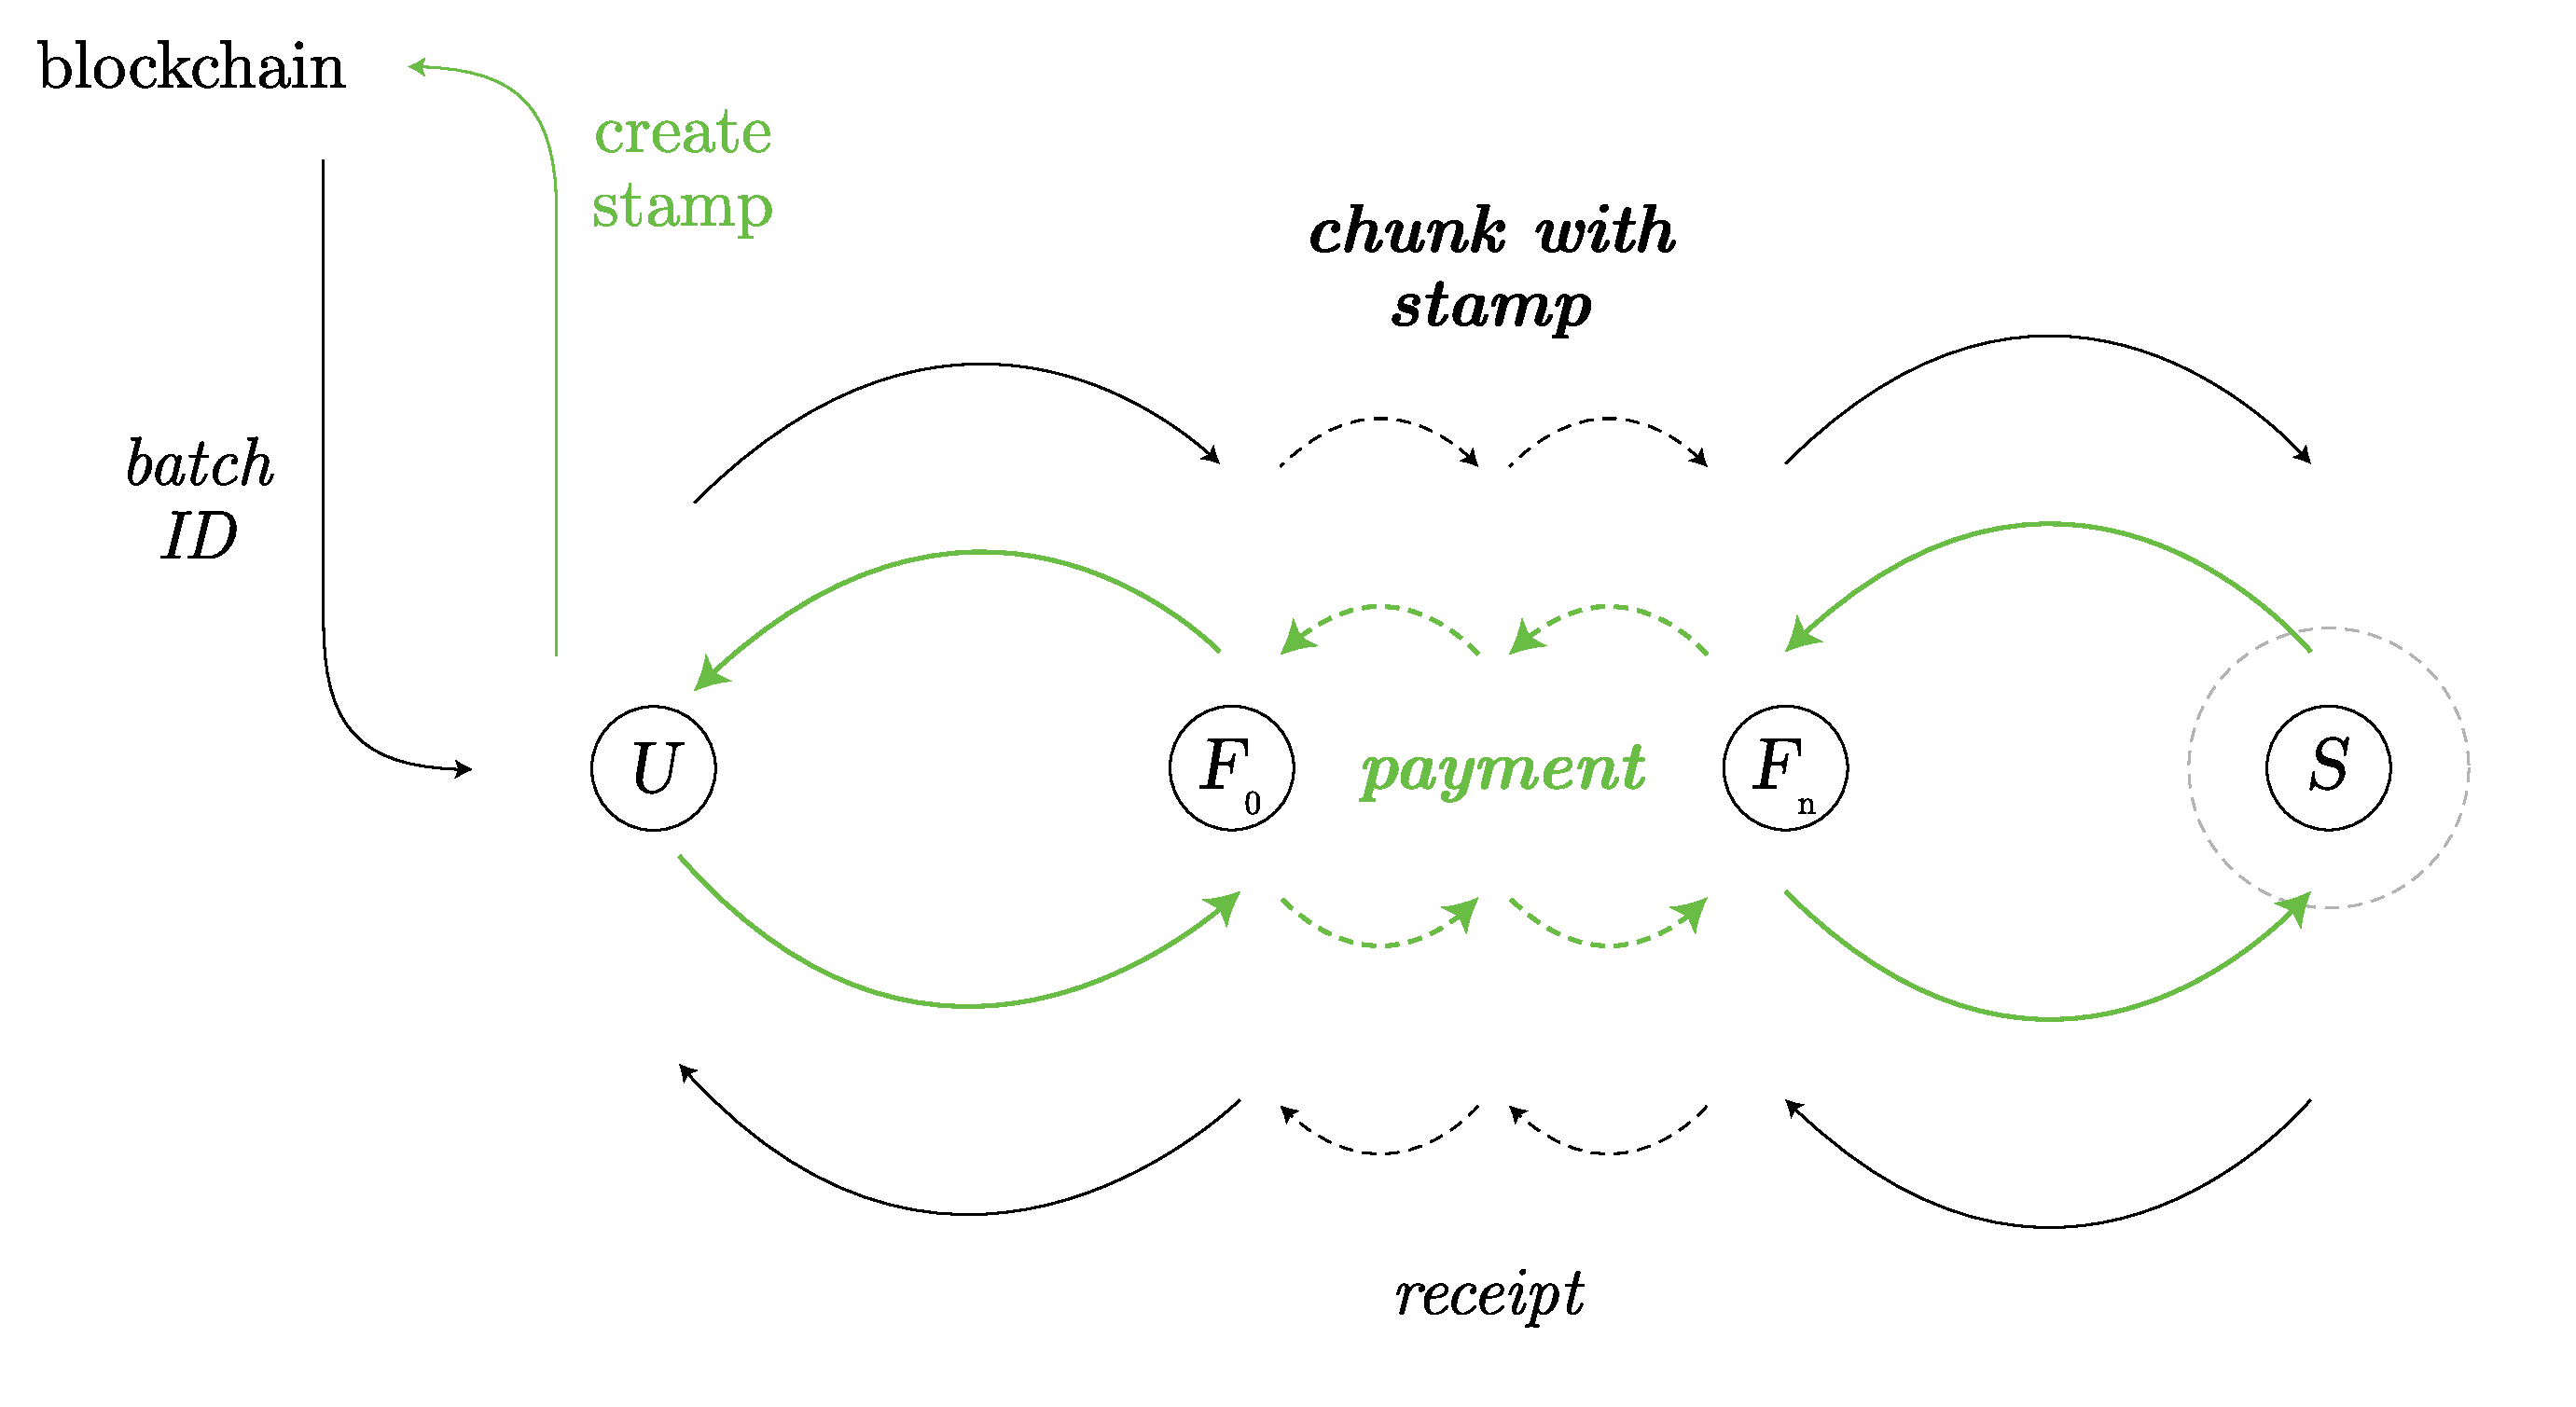
\includegraphics[width=\textwidth]{fig/postage-stamp.pdf}
\caption[Postage stamps]{Postage stamps are purchased in bulk on the blockchain and attached to chunks at upload. They are passed along the push-syncing route together and their validity is checked by forwarders at each hop. }
\label{fig:postage-stamps}
\end{figure}

The normalised per-chunk balance of a batch is calculated as the batch inpayment divided by the batch size in chunk storage slots. The chunk balance is interpreted as an amount pre-committed to be spent on storage. The balance decreases with time as if \emph{storage rent} was paid for each block at the price dictated by the price oracle contract.  

This system allows prepayment for storage without having to speculate on the future price of storage or fluctuations in the currency's exchange rate. At the cost of decreased certainty about the expiration date, one gains resilience against price volatility. On top of this, uploaders can enjoy the luxury of non-engagement by tying up more of the batch balance; while it serves as collateral against price increase, if that does not happen the funds can still be used up (for storing).


\subsection{Limited issuance}\label{sec:limited-issuance}

% \subsubsection{Issuing postage stamps}

Purchasing a postage batch effectively entitles the owner to issue a fixed amount of postage stamps against the batch ID called the \gloss{issuance volume} or \gloss{batch size}. It is restricted to the powers of 2 and is specified using the base 2 logarithm of the amount which is called \gloss{batch depth}. Storage slots of a batch are arranged in a number of buckets and are indexed within the bucket. The number of buckets is restricted to the powers of 2 and is specified using its base 2 logarithm called \gloss{uniformity depth}. The size limitation of a batch with batch depth $d$ and uniformity depth $u$ is equivalent to the conditions that 1) the bucket index ranges from 0 to $2^u-1$, 2) the within-bucket index ranges  from 0 to $2^{d-u}-1$ and 3) there are no duplicate indexes.  

While 1) and 2) is easily verifiable by any third party, 3) is not.
In order for index collisions to be detectable by individual storer nodes, uniformity depth must be large enough to fall within nodes' area of responsibility.
As long as this is maintained, all chunks in the same bucket are guaranteed to land in the same neighbourhood, and, as a result, duplicate assignments can be locally detected by nodes (see figure \ref{fig:over-issuance}).

In order to keep their stamps collision-free, uploaders need to maintain counters for how many stamps they have issued for each bucket of a batch and must not issue more than the allowed bucket size. 

\begin{figure}[!ht]
  \centering
    
\includegraphics[width=1\textwidth]{fig/batch-structure.pdf}
  \caption[Batch structure, uniformity and over-issuance]{Batches come with $2^u$ equal-sized buckets ($u$ is uniformity depth, orange circle) each containing an equal number of storage slots ($2^{d-u}$) adding up to batch capacity of $2^d$ chunks ($d$ is batch depth, red circle). Storage slots are indexed and the index is associated with a chunk via the stamp signature. Postage stamp over-issuance is detected locally by storer nodes as long as the buckets are deeper than their storage depth (green circle), as in the diagram on the left. In this case they will receive all the chunks that are correctly assigned to the relevant bucket (orange radii) and correctly identify collisions (red radii) by forbidding indexes that are either out of range ($\geq 2^{d-u}$) or multiply assigned. In contrast, the diagram on the right shows it is not possible for a node with storage depth 4 to identify duplicates for a batch with $u=2$.}
\label{fig:over-issuance}
\end{figure}    



In general, the most efficient utilisation of a batch is by filling each bucket fully. 
%
%
% \footnote{See appendix \ref{sec:batch-utilisation} for a detailed analysis of batch utilisation.
% \subsubsection{Efficiency of batch utilisation}
% }
%       
Continued non-uniformity (i.e., \emph{targeted issuance}) leads to underutilised batches, and therefore a higher unit price for uploading and storing each chunk. This feature has the desired side effect that it imposes an upfront cost to non-uniform uploads: the more concentrated the distribution of chunks of an upload, the more storage slots of the postage batch remain unused. In this way, we ensure that targeted denial-of-service attacks against a neighbourhood (i.e., uploading a disproportionate number of chunks in a particular address range) is costly since the \emph{inert cost} (due to the degree of under-utilisation of the batch) is exponential in the depth of the skew.

Beyond DoS protection, postage stamps can serve as a \emph{fiduciary signal} indicating how much it is worth for a user to persist a chunk in Swarm. In particular, the per-chunk balance of batches can provide the differential a priori bias determining which chunks should be protected from garbage collection in the absence of evidence to predict their profitability from swap. 



\subsection{Rules of the reserve}\label{sec:reserve}

% \subsubsection{Batch balance, rent and expiry}\label{sec:rent-expiry}

The \gloss{reserve} is a fixed size of storage space dedicated to storing the chunks in the node's \gloss{area of responsibility}. Chunks in the reserve are the chunks that are protected against garbage collection with valid postage stamps. When batches expire, i.e., their balance is completely depleted, the chunks they stamped are no longer protected from eviction. Their eviction from the reserve frees up some space that can accommodate new or farther chunks belonging to valid batches.


From the point of view of incentives, chunks which are of the same proximity order and the same batch are equivalent. When it comes to eviction due to batch expiry, these equivalence classes, called \gloss{batch bins} are handled as one unit: the chunks in a batch bin are evicted from the reserve and inserted to the cache in one atomic operation. 

Assuming a global oracle for the unit price of rent and a fixed reserve capacity  prescribed for nodes, the content of the reserve is coordinated with  a set of constraints on batch bins called the \gloss{rules of the reserve}:
\begin{itemize}[noitemsep]
    \item[--] if a batch bin of a certain PO is reserved then the batch bins are reserved also for all closer bins (higher PO). 
    \item[--] if a batch bin is reserved at a certain proximity order (PO), then all the batch bins at the same PO belonging to batches with a greater per-chunk balance are also reserved. 
    \item[--] the reserve should not exceed capacity.
    \item[--] the reserve is maximally utilised, i.e, cannot be extended and have 1-3 remain true.
\end{itemize}

The first rule means the reserve is closed upwards for PO, which encodes a global preference for  chunks closer to the node's address. This is incentivised by routing: keeping the closest chunks, a node will maximise the number of receipts it can issue and the number of retrieve requests it can respond to and at the same time provides the widest coverage within the neighbourhood even after the neighbourhood is no longer supporting the desired redundancy.

The second rule expresses the constraint that the reserve for a PO is upward closed for per-chunk balance, which encodes a secondary preference among chunks of the same proximity for those stamped using a batch with higher per-chunk balance. This is incentivised by the differential absolute profit chunks promise: due to the  constraint that balances are not revocable, chunks with higher balance expire later and therefore contribute more to storers' absolute profit than those expiring earlier despite the same rent paid during their period of validity.%
%
\footnote{Note that even if there was no scheme for redistributing postage revenue and the inpayments are frozen/burnt, this strategy is still mildly incentivised in as much as it is aligned with token-holders interest: batches with higher balance exert more deflationary force on the token (per chunk, i.e, the unit of invested resource) by keeping their balance frozen which is expected to realise in a proportional price increase.}


\begin{figure}[!ht]
  \centering
    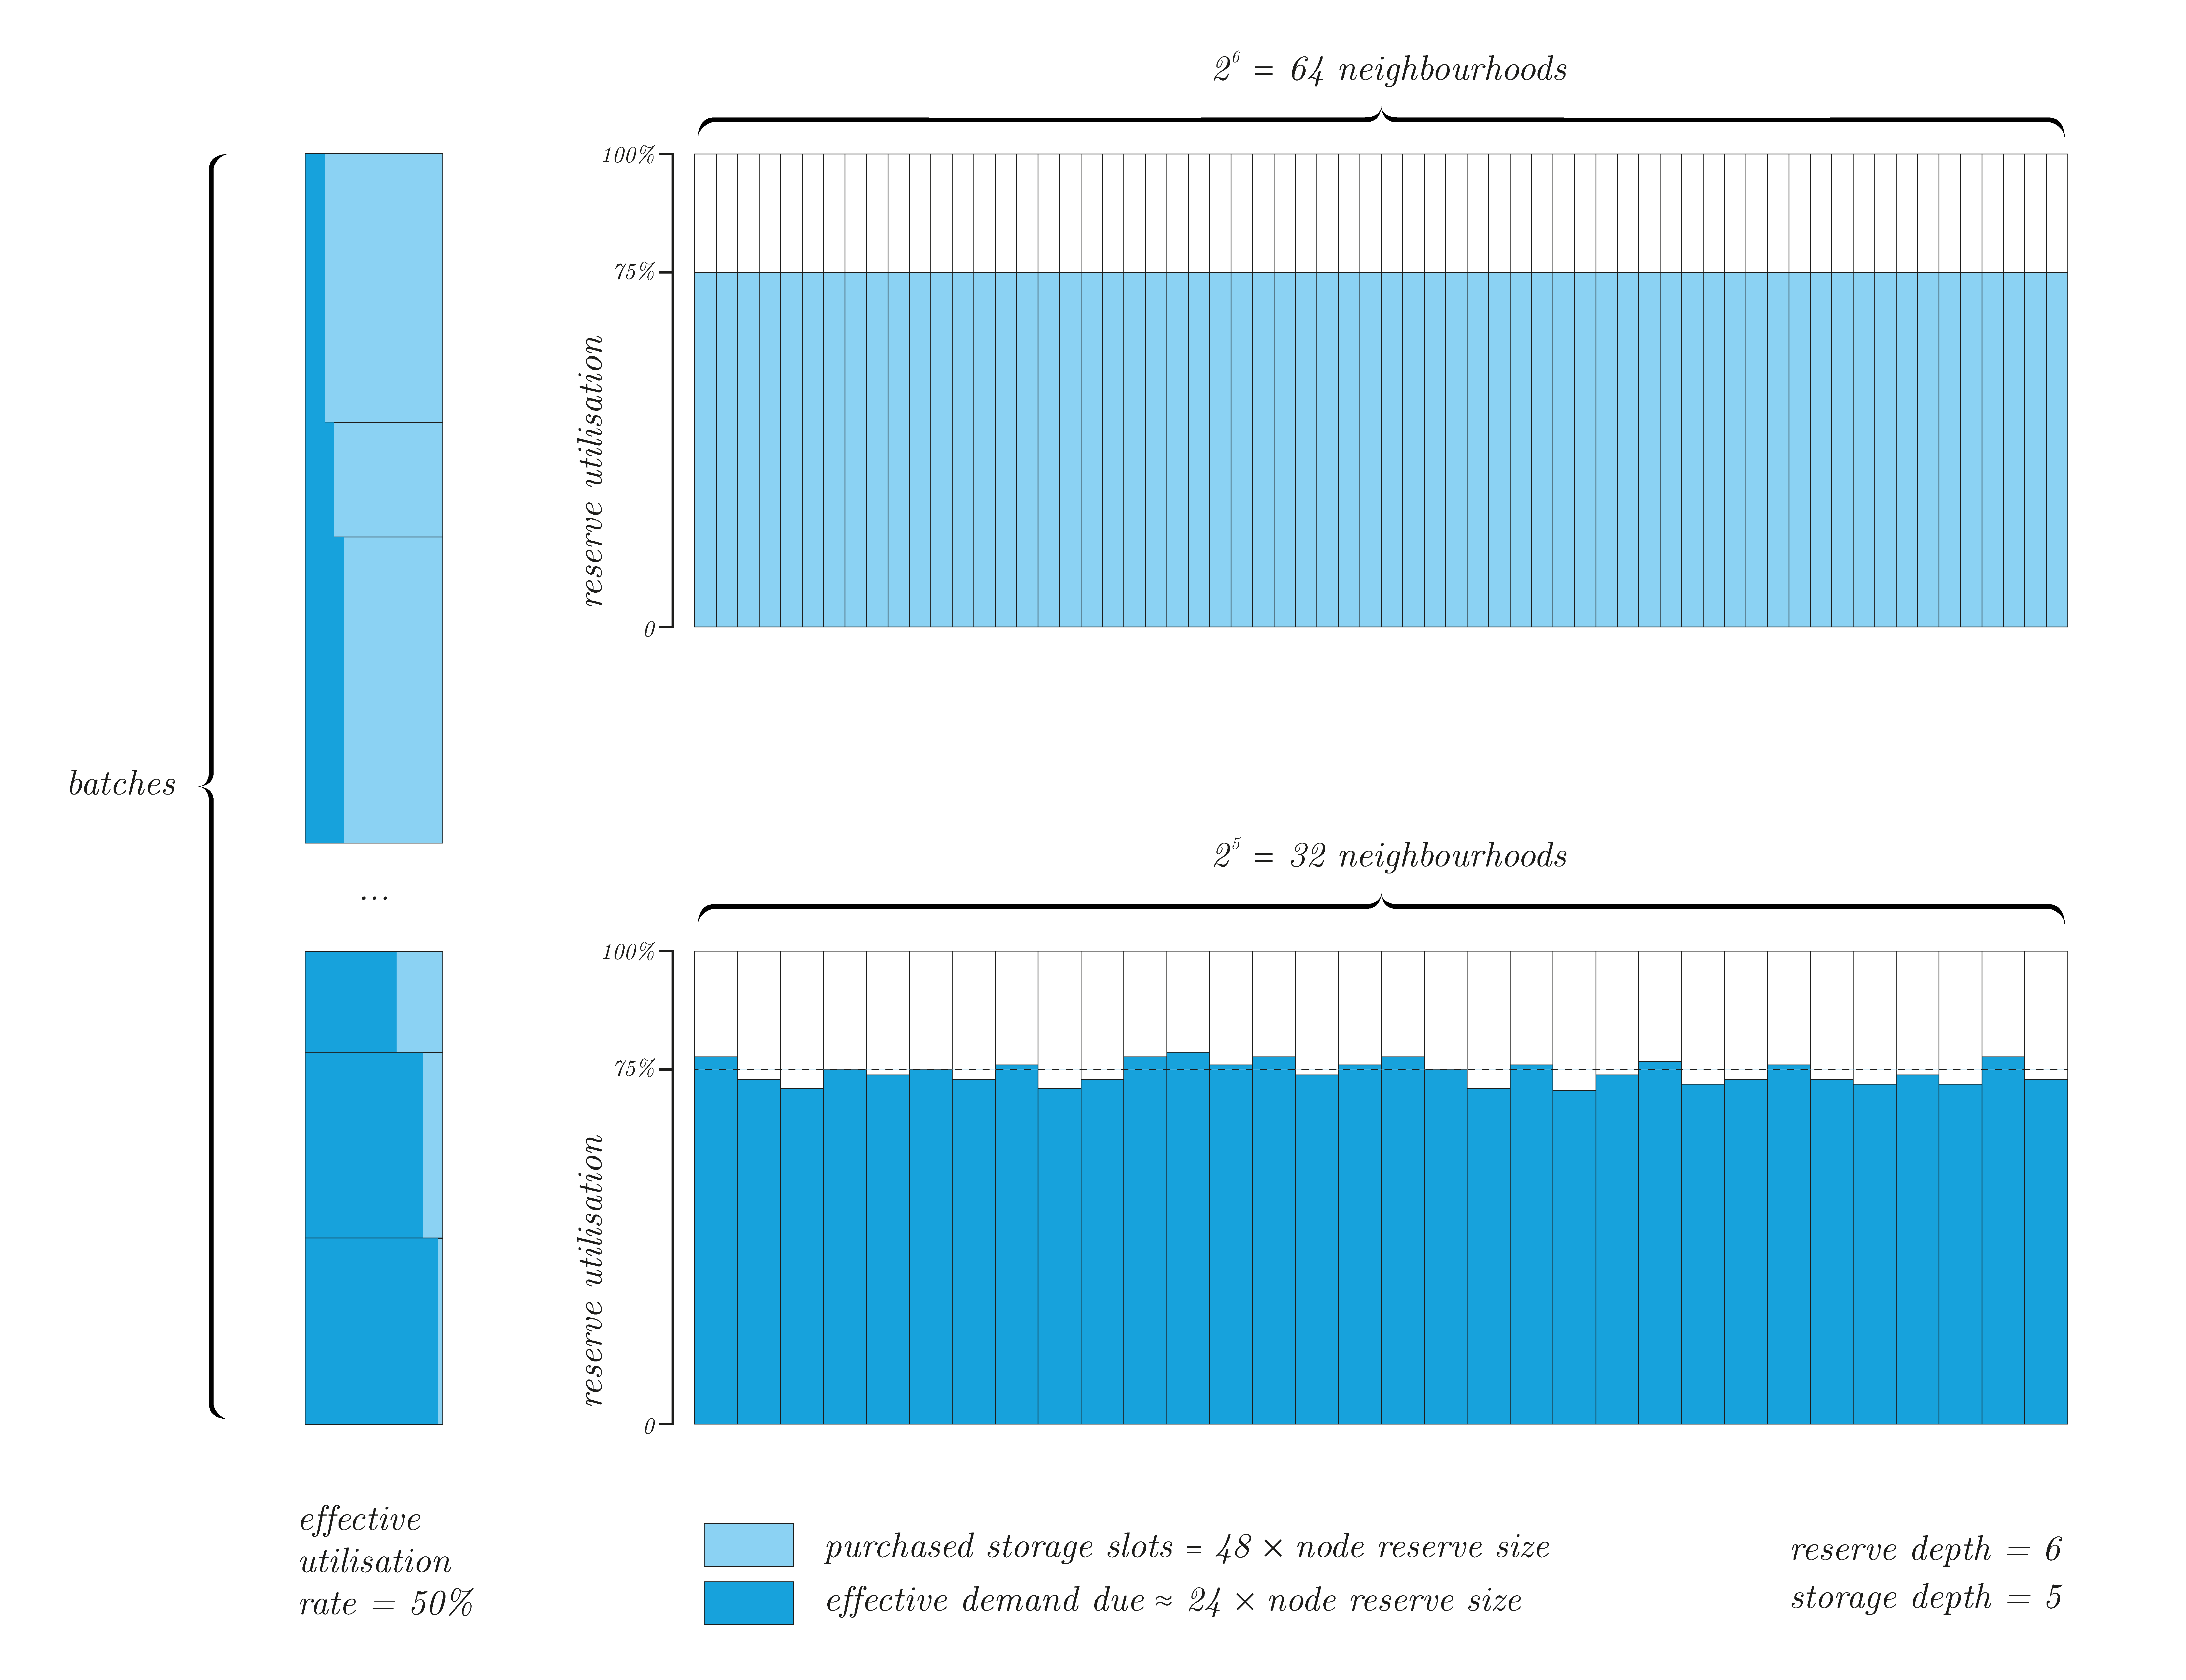
\includegraphics[width=.9\textwidth]{fig/supply-demand.pdf}
  \caption[Reserve capacity]{Potential demand for chunk storage is expressed by the total size of all batches with non-zero balance on the blockchain (left). The lower bound on neighbourhood depth to store this capacity is the reserve depth (top right). Storage depth marks the effective volume of chunks uploaded and stored in a neighbourhood's reserve (bottom right). The difference between them is a result of partial batch utilisation. The uniformity of the volume of chunks across neighbourhoods is incentivised by the efficient utilisation of postage batches.}
\label{fig:reserve-capacity}
\end{figure}    

When a new chunk arrives in swarm through pull-sync, push-sync or upload, the validity  of the attached  postage stamp is verified. If the PO of the chunk is lower than the batch depth, the node inserts the chunk into the  garbage collection index, otherwise it is by definition in the reserve. 
If the reserve size is above capacity, a number of batch bins are identified so that their total size covers the excess so that after these batch bins are \emph{evicted} from the reserve, the reserve size will be within capacity. 


\subsection{Reserve depth, storage depth, neighbourhood depth}\label{sec:depths}



\subsubsection{Reserve depth}

The potential demand for chunks to be stored in the DISC is quantified by the total storage slots of valid batches. This is calculated as the sum of the sizes of non-expired batches. Since the batches and their balances are recorded in the postage contract, the reserved DISC size is under consensus.%
%
\footnote{The volume is best explicitly maintained by the contract by adding the size of newly created batches and deduct the sizes of newly expired batches. DISC reserve size is updated each time a batch is created or topped up and expired batches are removed during each redistribution round, executed as part of the process triggered by the claim transaction.}  

The base 2 logarithm of the DISC reserve size rounded up to the nearest integer is called the \gloss{reserve depth}. The reserve depth is the shallowest PO such that disjoint neighbourhoods of this depth are collectively able to accommodate the volume of data corresponding to the total number of chunks paid for, assuming that nodes in the neighbourhood have a fixed prescribed storage capacity to store their share of the reserve. 

The reserve depth is also the \emph{safe lower bound} for pull-syncing, i.e, the farthest bin a neighbourhood needs to synchronise to guarantee storing the reserve.
Conversely, if any neighbourhood marked by reserve depth has no nodes in it, the swarm is not working correctly, i.e., chunks with valid stamps are not protected from getting lost. See figure \ref{fig:depths}.

\subsubsection{Storage depth}

The \gloss{effective demand} for chunks to be stored in the DISC is the total number of chunks actually uploaded. While each chunk in the reserve has a valid postage batch and therefore is assigned to a storage slot, a postage batch can always have some of its storage slots unassigned. This entails that the number of chunks actually stored in the DISC can in fact be a fraction of the DISC reserve size. 

The effective area of responsibility is  marked by the proximity order of the farthest batch bin of the reserve assuming the node complies with the rules of the reserve. 

A node's \gloss{storage depth} is defined as the shallowest \emph{complete} bin, i.e., the lowest PO that compliant reserves stores all batch bins at. Unless the farthest bin in the node's reserve is complete, the storage depth equals the reserve's edge PO plus one.

The storage depth is the \emph{optimal lower bound} for pull-syncing, i.e, the farthest bin the node needs to synchronise with its neighbours to achieve maximum reserve   utilisation.%
%
\footnote{The nodes will have full connectivity up to the shallowest bin that they are pull syncing. This choice is incentivised by the risk of having two disjoint connected sets of pull-syncing nodes resulting in non-consensual reserve. As a consequence, we can say that storage depth is an upper bound on the depth of full connectivity.}
%
Maximum reserve utilisation should be incentivised as part of the storage incentives. 

% See figure \ref{fig:reserve-depth-vs-storage-depth}.

% \begin{figure}[!ht]
%   \centering
%     % \includegraphics[width=\textwidth]{fig/reserve-depth-vs-storage-depth.pdf}
%   \caption[Reserve depth vs storage depth]{Reserve depth vs storage depth.}
% \label{fig:reserve-depth-vs-storage-depth}
% \end{figure}    




% \subsubsection{Batch utilisation rate}\label{sec:utilisation-rate}

The gap between actual storage depth and the  reserve depth exists because of the bulk purchase of stamps. Since entire batches of stamps reserve storage slots that are assigned to  chunks only at later times when they are actually uploaded, the batch \emph{utilisation rate} can be substantially less than 1%
% (see appendix \ref{sec:batch-utilisation})%
. Storage depth and reserve depth are the same only if all batches are fully utilised. 


\subsubsection{Neighbourhood depth}

Swarm's requirements on local replication is that each neighbourhood designated by the storage depth contains at least four nodes. 
If neighbourhoods were made of one node, then the outage of that one node will make  the chunks in the node's area of responsibility not retrievable.
With two nodes in a neighbourhood, we significantly improve resilience against ad-hoc outages, but because of connectivity latencies a two-peer neighbourhood still displays unstable user experience.
The ideal scenario is to have four nodes per full connectivity neighbourhood, which prompts the following definition: \gloss{neighbourhood depth} for a particular node is the highest PO $d$ such that the address range designated by the $d$-bit-long prefix of the node's overlay contains at least 3 other peers.


Figure \ref{fig:depths} details the potential relative orders of the three depths and their consequences on the health, efficiency and redundancy of the swarm.

\begin{figure}[!ht]
  \centering
    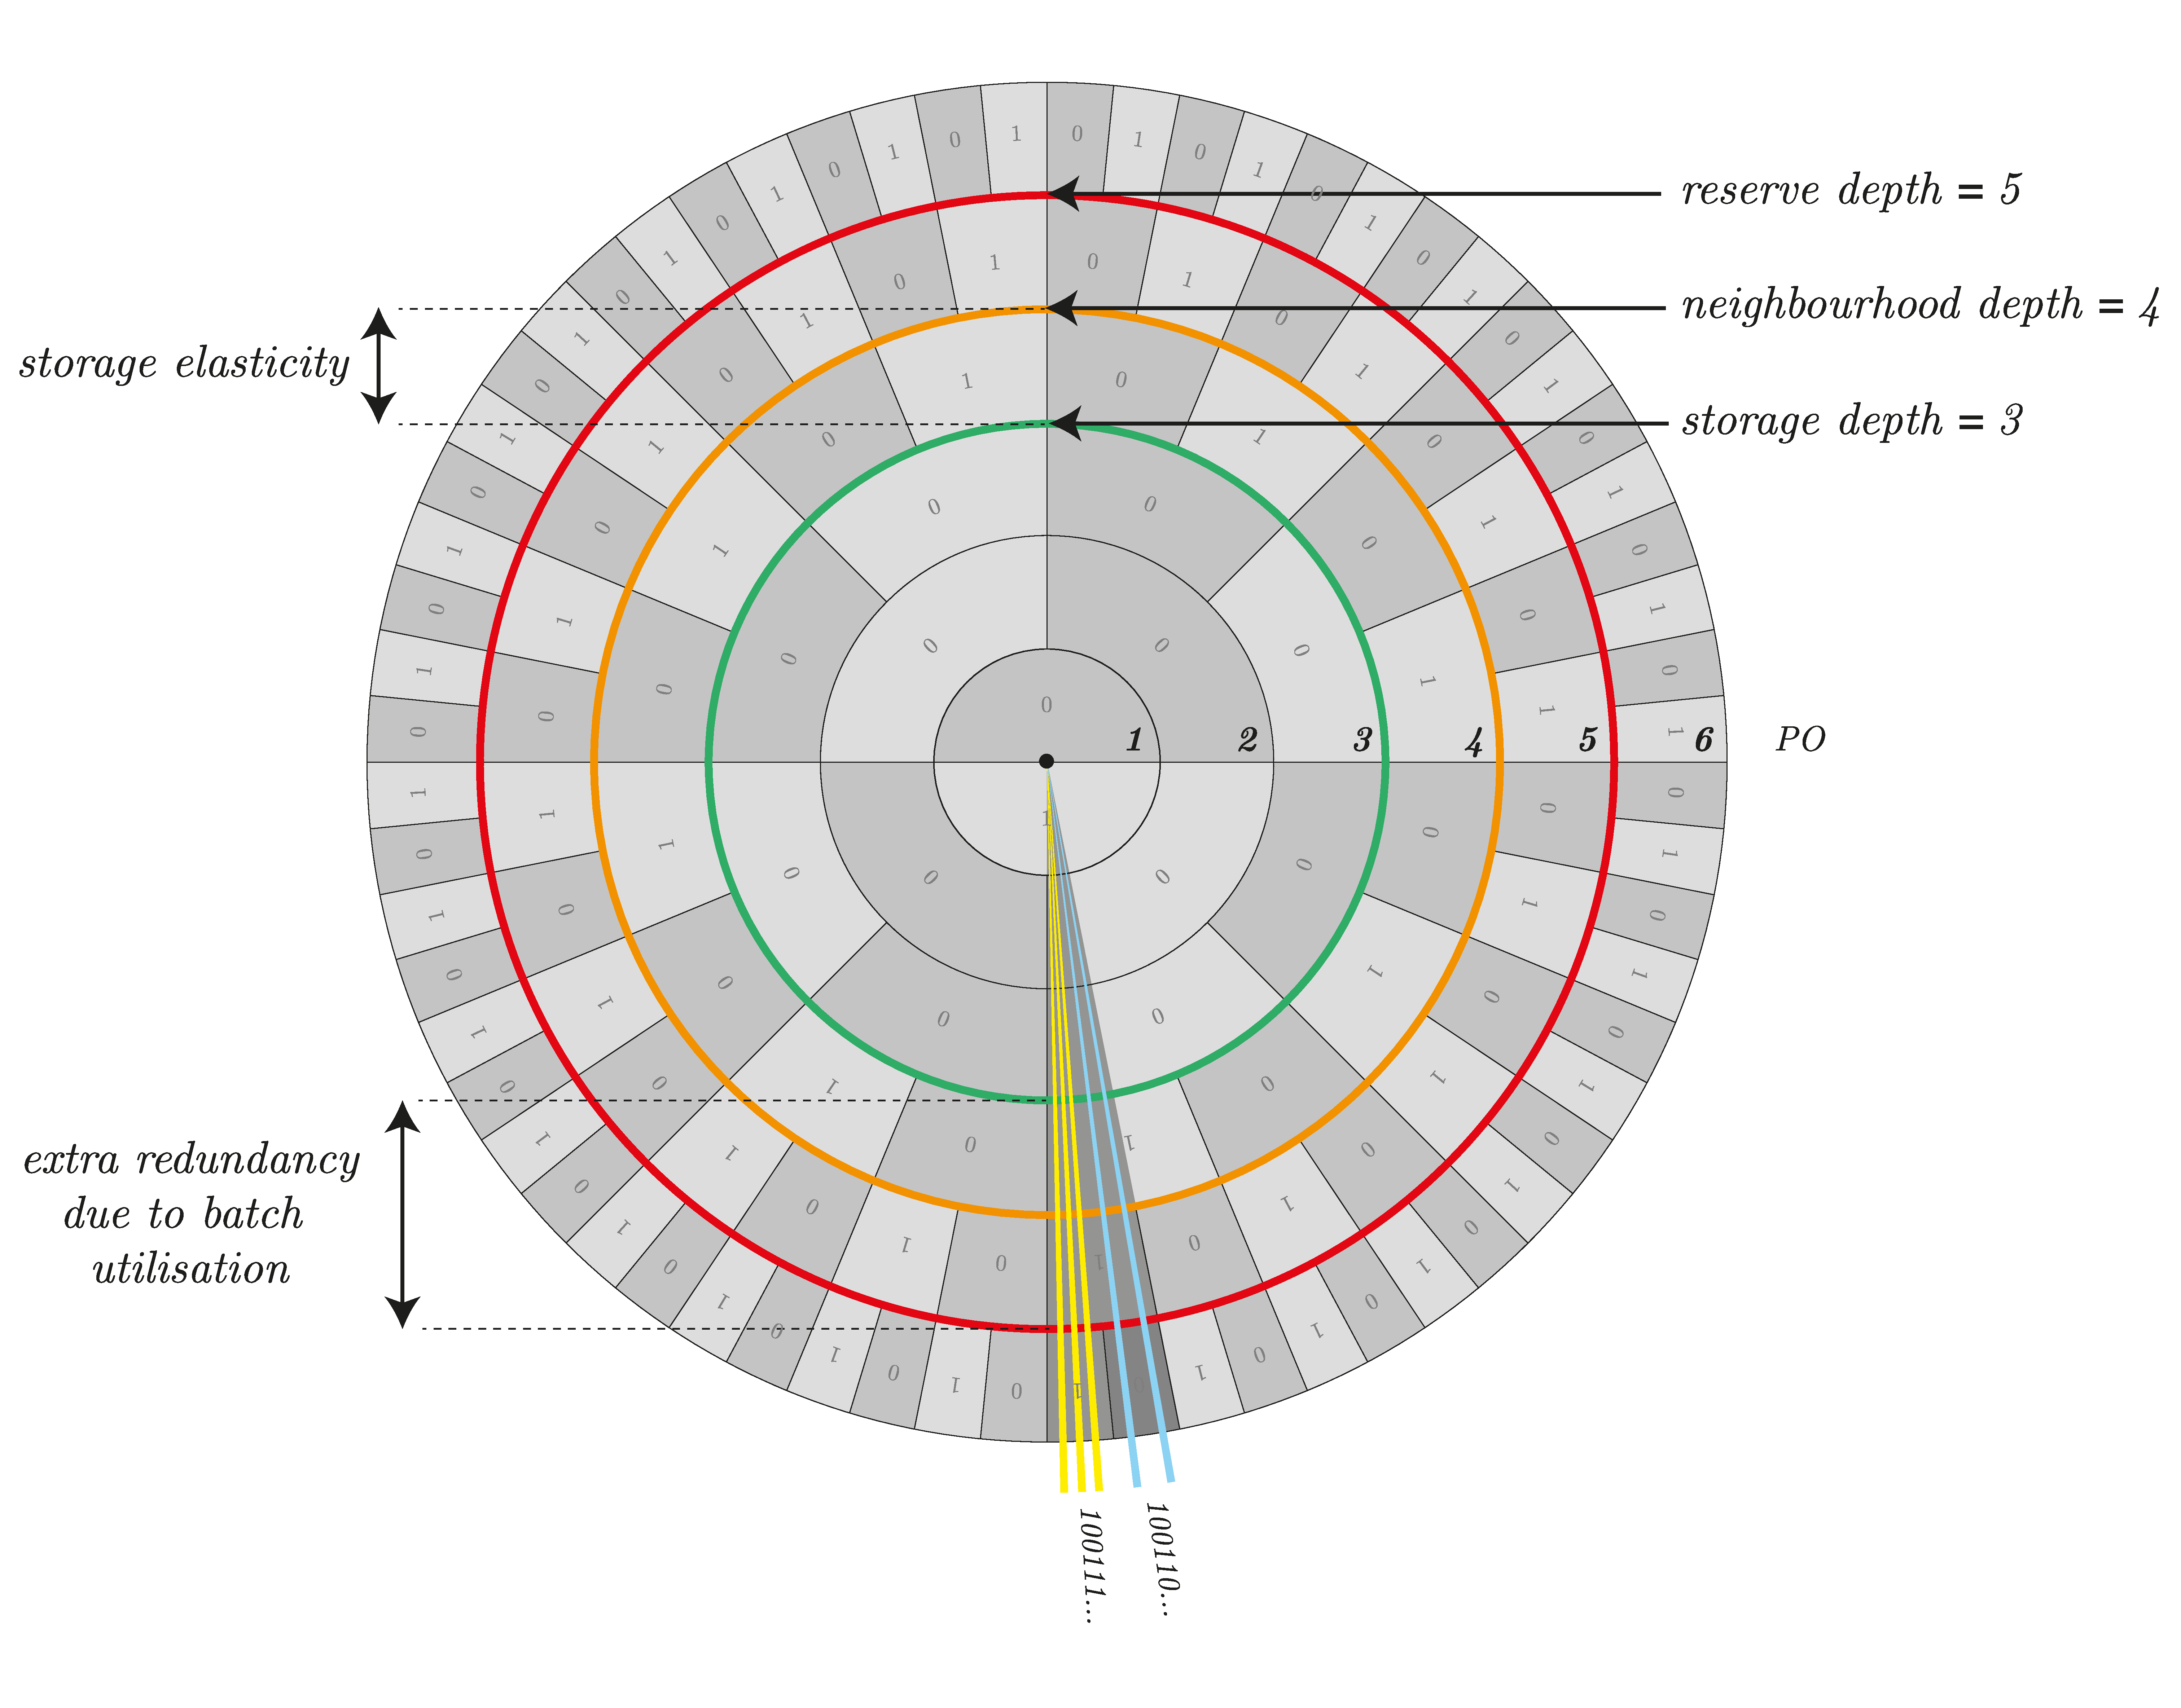
\includegraphics[width=.7\textwidth]{fig/depths-2.pdf}
  \caption[Depths]{The 3 depths (reserve, storage and neighbourhood) express the order of magnitude of reserved capacity (potential demand, red circle), uploaded chunks (effective demand, green circle) and the number of nodes (effective supply, orange circle), respectively. Their possible orderings express different scenarios with characteristic impact on data availability. Storage depth cannot be greater than reserve depth. A gap between storage depth and reserve depth quantifies the average batch utilisation rate. The gap between storage depth and a deeper neighbourhood depth quantifies the elasticity of the storage: the difference expresses how many times the effective volume can double before redundancy goes below required. While such oversupply may be anticipatory of growth in demand, if neighbourhood depth remains deeper than storage depth long term, it may indicate excessive profits. The opposite order indicates undersupply (redundancy below the desired level).}
\label{fig:depths}
\end{figure}    
%%%%%%%%%%%%%%%%%%%%%%%%%%%%%%%

% In the introduction we concluded that Swarm needs to have a subsystem for users to signal the importance/relevance of chunks. Postage stamps (and batches) were presented as a framework to implement storage incentives to ensure rarely accessed content remains available. 

%%%%%%%%%%%%%%%%%%%%%%%%%%%%%%%%%%%%%%%%%%%%%%%%%%%%%%%
\section{Fair redistribution}\label{sec:redistribution}


The system of positive%
%
\footnote{The concept of \emph{positive incentives} refers to a scheme whereby providers of a service are entitled to reward but there is no loss involved if they discontinue their service or are not online.}
%
storage incentives in Swarm is concerned with redistributing  to storage providers the BZZ tokens that uploaders deposited within the postage contract.%
%
\footnote{As explained earlier, uploaders pay in an unwithdrawable amount to the postage contract which serves as the balance to pay storage rent. In exchange they obtain the right to issue a fixed number of postage stamps which they attach to chunks they want the network to store.}
%
The overall balance on the contract covers the \gloss{reward pot} which represents the total \gloss{storage rent} cumulated over all postage batches for a particular period. The storage rent must be redistributed to storage providers in a way that guarantees that their earnings are proportional to their contribution weighing in storage space, quality of service and length of commitment.

The procedure for redistribution is best conceived of as a game orchestrated by a suite of smart contracts on the blockchain. Nodes earn the right to play through participation in storing and syncing chunks. 
The winners claim their reward by sending a transaction to the game contract. 

In section \ref{sec:uniformity-pot}, we formulate the idea of redistribution in terms of probabilistic outpayments to allow an easy proof of fairness. Next, in \ref{sec:mechanics}, we introduce the mechanics of the redistribution game.
Then, in \ref{sec:staking} and \ref{sec:por} we explain how we enforce maximum utilisation of dedicated storage for persisting  relevant content redundantly. We conclude in \ref{sec:price-oracle} by discussing how to read certain aspects of the game as price signals that render the network self-regulating through automatic price discovery. 

\subsection{Neighbourhoods, uniformity and probabilistic outpayments}\label{sec:uniformity-pot} 

In this section we argue that the efficient use of postage batches incentivises a balanced chunk distribution which in turn gives rise to uniform storage depth across neighbourhoods. We then explain how this enables a fair system of redistribution using probabilistic outpayments.
% \subsubsection{Uniformity}


Assuming an oracle that sets the unit price of storage, the storage rent due for a period of time for a batch can be calculated. The number of rent units for a batch is the result of multiplying the size of the batch with the number of blocks in the period. The price of rent is calculated from the number of rent units multiplied by the unit price.%
%
\footnote{If this theoretical amount is less than the the current balance of the batch, then the batch is expired and the effective rent is only the remaining balance.}
%
The total storage rent cumulated over all batches for the period between two outpayments constitutes the \emph{reward pot} for the round.

Instead of dividing the reward pot among neighbourhoods regularly, the entire reward pot can be transferred to (representative nodes in) one target neighbourhood in each round. This probabilistic outpayment scheme is fair on the level of neighbourhoods as long as we can make sure that over a large number of rounds the probability with which a  
neighbourhood is selected as the target corresponds to its relative contribution to the overall network storage. Given a constant prescribed reserve capacity and replication of the reserve content by nodes in a neighbourhood, each neighbourhood defined by storage depth contributes equally to the network. 

In section \ref{sec:postage-stamps}, we wrote that uploaders are strongly incentivised to use their postage batch in a way that the chunks they stamp with it are uniformly distributed across the address space. This being true of all batches creates a situation that chunks are uniformly distributed across the DISC. In particular, the sets of chunks sharing a prefix are expected to be roughly equal in size. Therefore we expect nodes to fill their prescribed reserve capacity with chunks at the same proximity order, irrespective of their location in the address space, i.e., the storage depth is uniform across  nodes and therefore across neighbourhoods.%
%
\footnote{Differences do occur due to variance but over many rounds, deviation from the mean is meant to be independent of the location.}
%
With neighbourhoods at equal depth, uniform sampling of neighbourhoods can be modelled by choosing the neighbourhood which contains an anchor (called the \emph{the neighbourhood selection anchor}%
%
% \footnote{one of the random nonces (see definition \ref{def:nonce-round}) from the \emph{random seed} of the round, see appendix \ref{sec:randomness}.}
%
) randomly dropped in the address space (see figure \ref{fig:neighbourhood-selection}).


\begin{figure}[!ht]
  \centering
    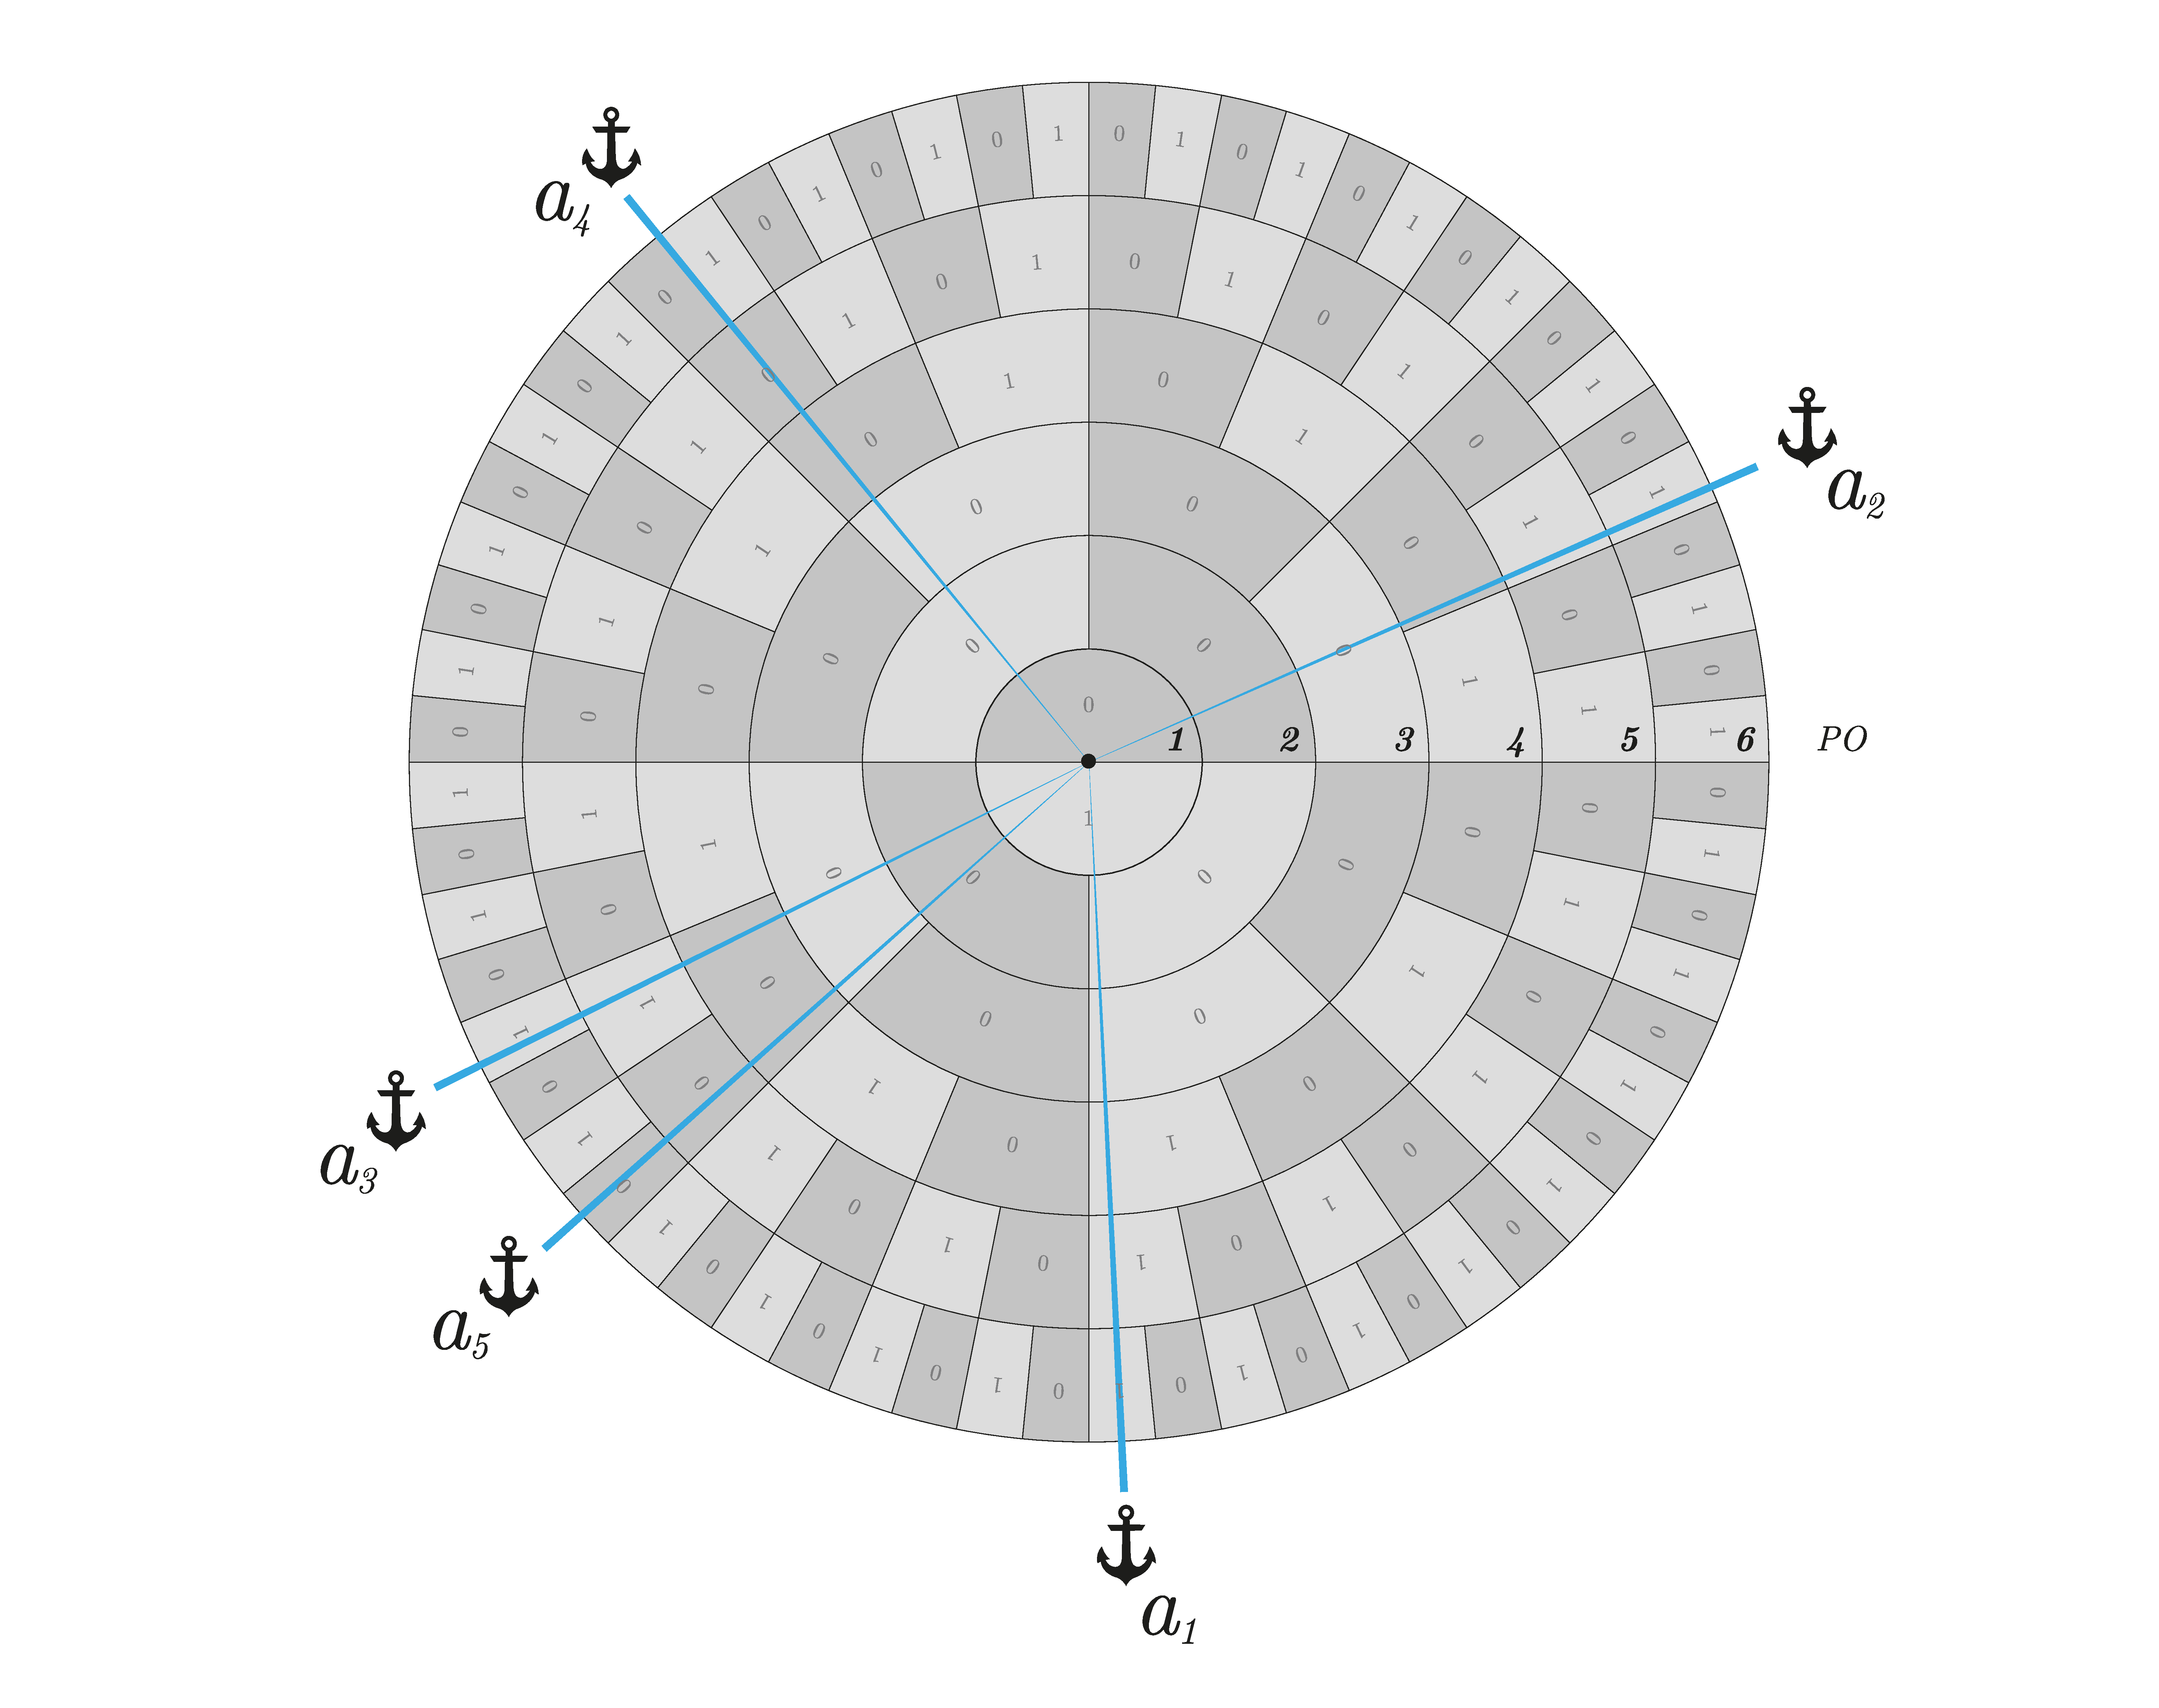
\includegraphics[width=\textwidth]{fig/nhd-selection.pdf}
  \caption[Neighbourhood selection and pot redistribution]{Neighbourhood selection and pot redistribution. The winning locality is selected by the neighbourhood selection anchor. Neighbourhoods that contain the anchor within their storage depth are invited to submit an application by committing to a consensual reserve sample. }
\label{fig:neighbourhood-selection}
\end{figure}    

    


\subsection{The mechanics of the redistribution game}\label{sec:mechanics}

The cooperation of peers to redundantly store for the network's benefit is underpinned by a \gloss{Schelling game}
% (defined formally in appendix \ref{sec:redistribution-game}) 
aimed at proving that the peers agree on the chunks they need to store and they do, in fact, store them. The redistribution game itself is orchestrated by the game contract, one of the building blocks of the system of 4 smart contracts which collectively drive the swarm storage incentive system (see figure \ref{fig:smart-contracts}):

\begin{itemize}
    \item[--] Postage contract -- serving as the batch store to sell postage batches to uploaders, keeping track of batch balances, batch expiry, storage rent and the reward pot itself.
    \item[--] Game contract -- orchestrates the redistribution rounds interacting with potential winners accepting commit, reveal and claim transactions from storage providers in selected neighbourhoods.
    \item[--] Staking contract -- operates a stake registry, maintaining committed stake and stake balance for nodes by their overlay; enables freezing and slashing of stake as well as withdrawal of surplus balance for stakers.
    \item[--] Price oracle -- maintains the unit price of  storage rent, accepts signals from the game contract to dynamically adjust according to supply and demand and provides current price oracle service for the other three contracts.
\end{itemize}


\begin{figure}[!ht]
  \centering
     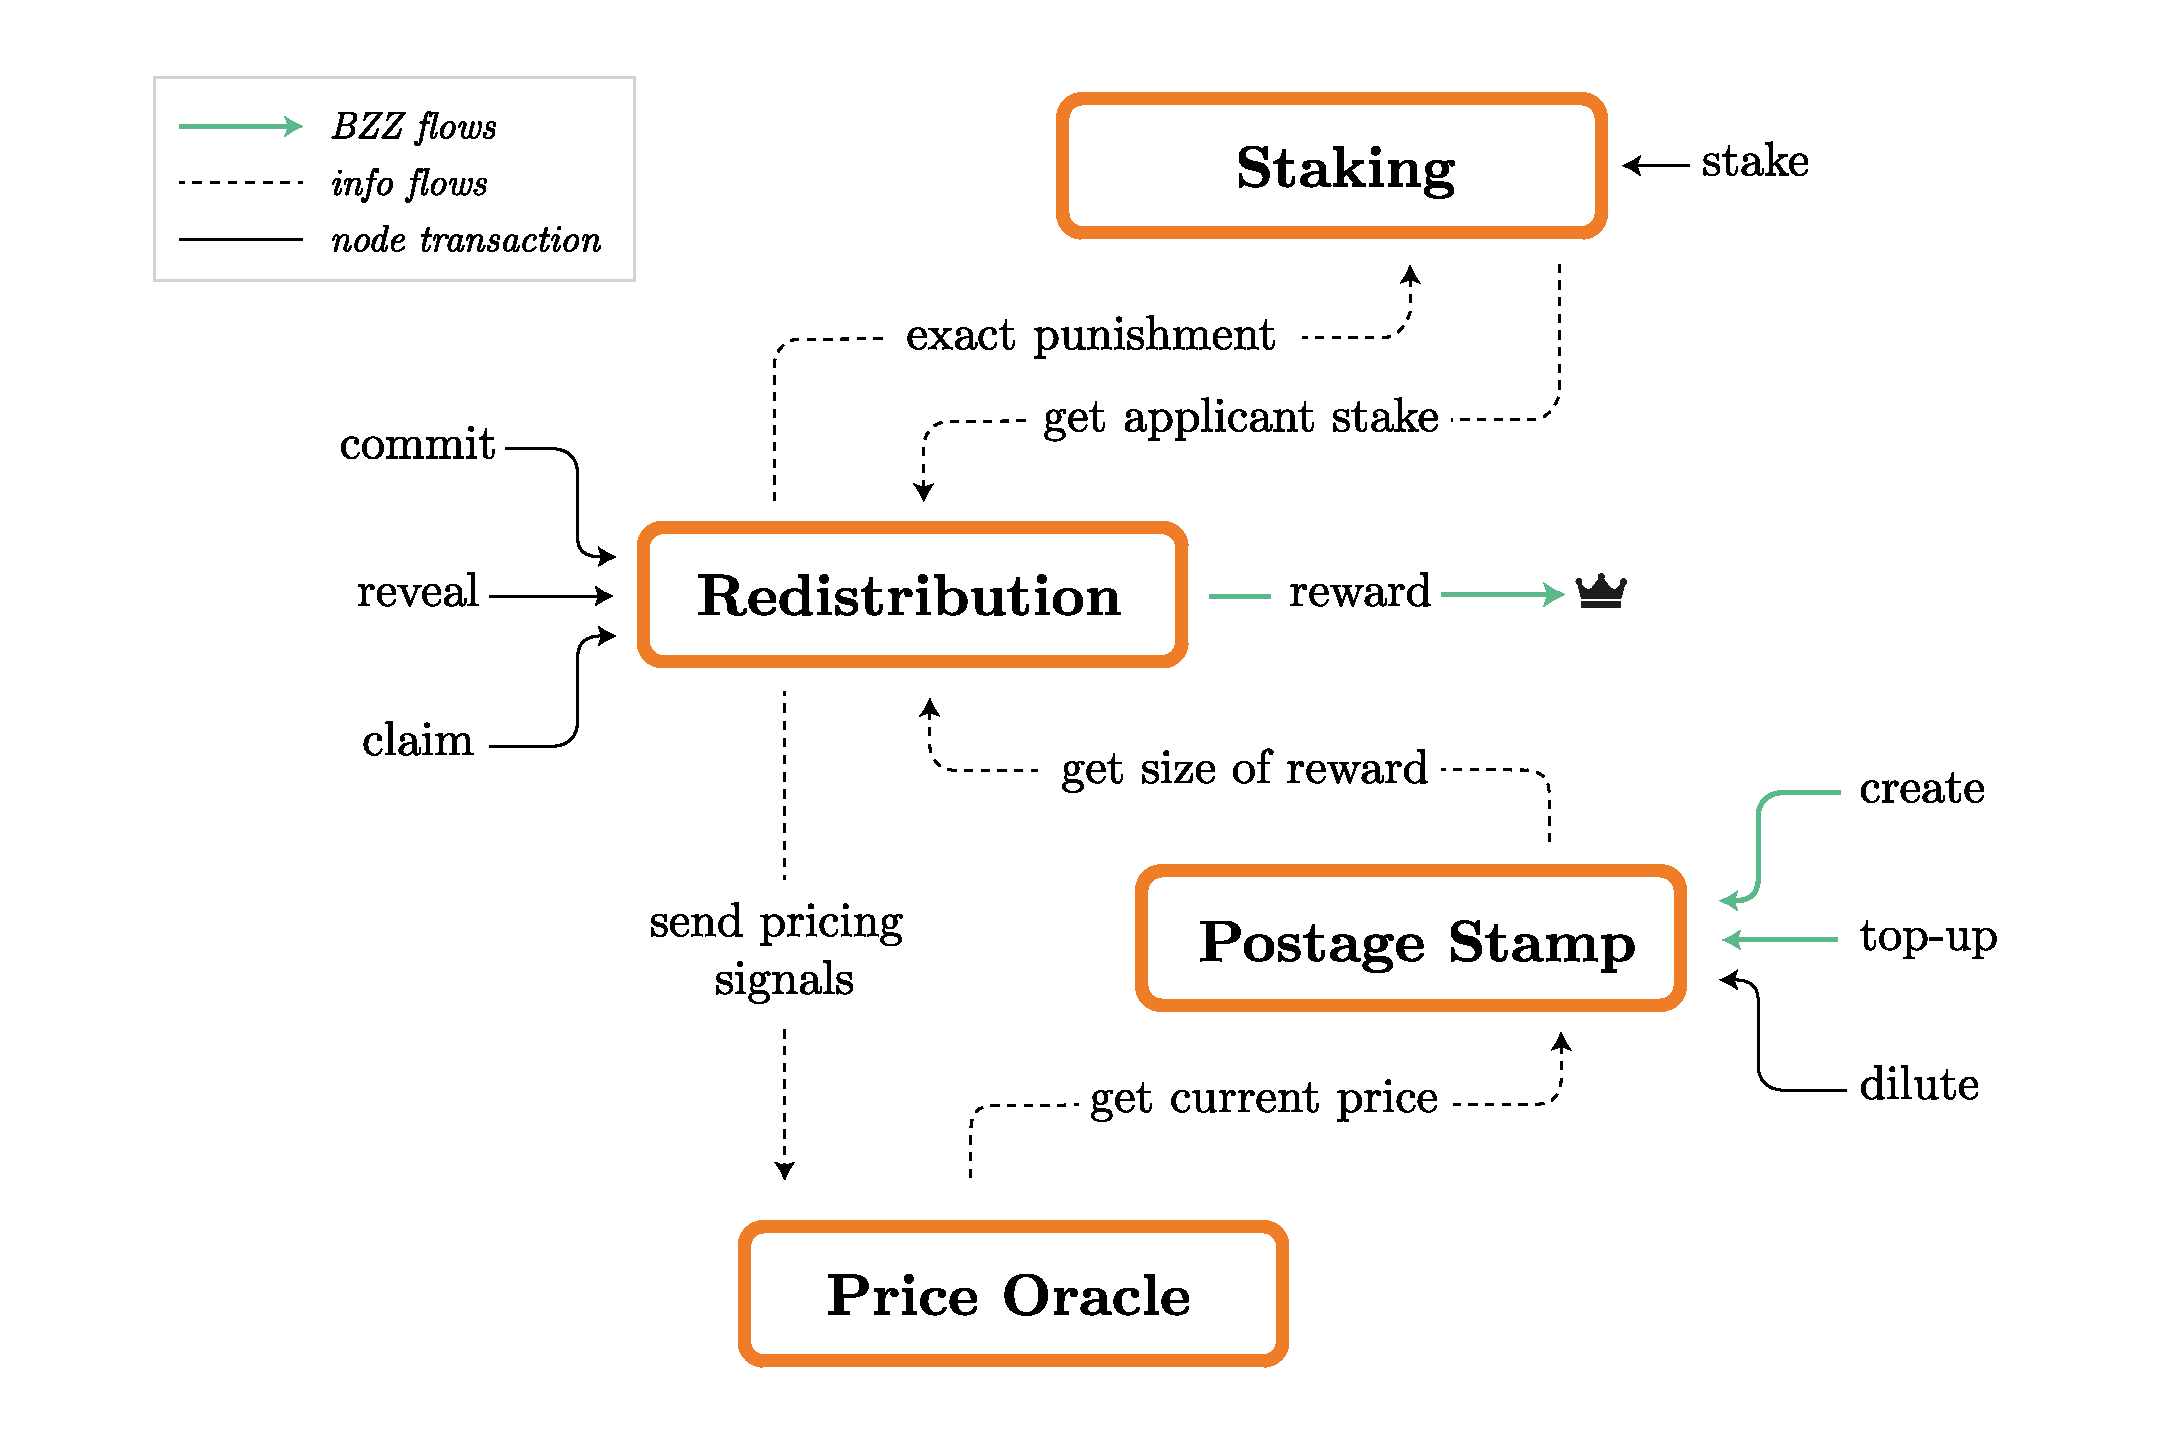
\includegraphics[width=\textwidth]{fig/smart-contract-interaction.pdf}
  \caption[Interaction of smart contracts for swarm storage incentives]{Interaction of smart contracts for swarm storage incentives. The figure shows with the dotted line the information flow between the four contracts comprising the storage incentive smart contract suite as well as the public transaction types they accept. }
\label{fig:smart-contracts}
\end{figure}    

The game is structured as a sequence of \emph{rounds}. Each round lasts for a fixed number of blocks and recur periodically. A round consists of 3 phases: \emph{commit}, \emph{reveal}, and \emph{claim}.%
%
\footnote{The commit and reveal phases are one quarter of the round length while the claim phase is one half.
}
%
The phases are named after the type of transaction the smart contract expects during that phase, and that nodes from the selected neighbourhood need to submit.%
%
\footnote{Both commit and reveal are simple and cheap transactions. The only expensive transaction is claim but that only the winner needs to submit.}
%
See figure \ref{fig:phases}

\begin{figure}[!ht]
  \centering
    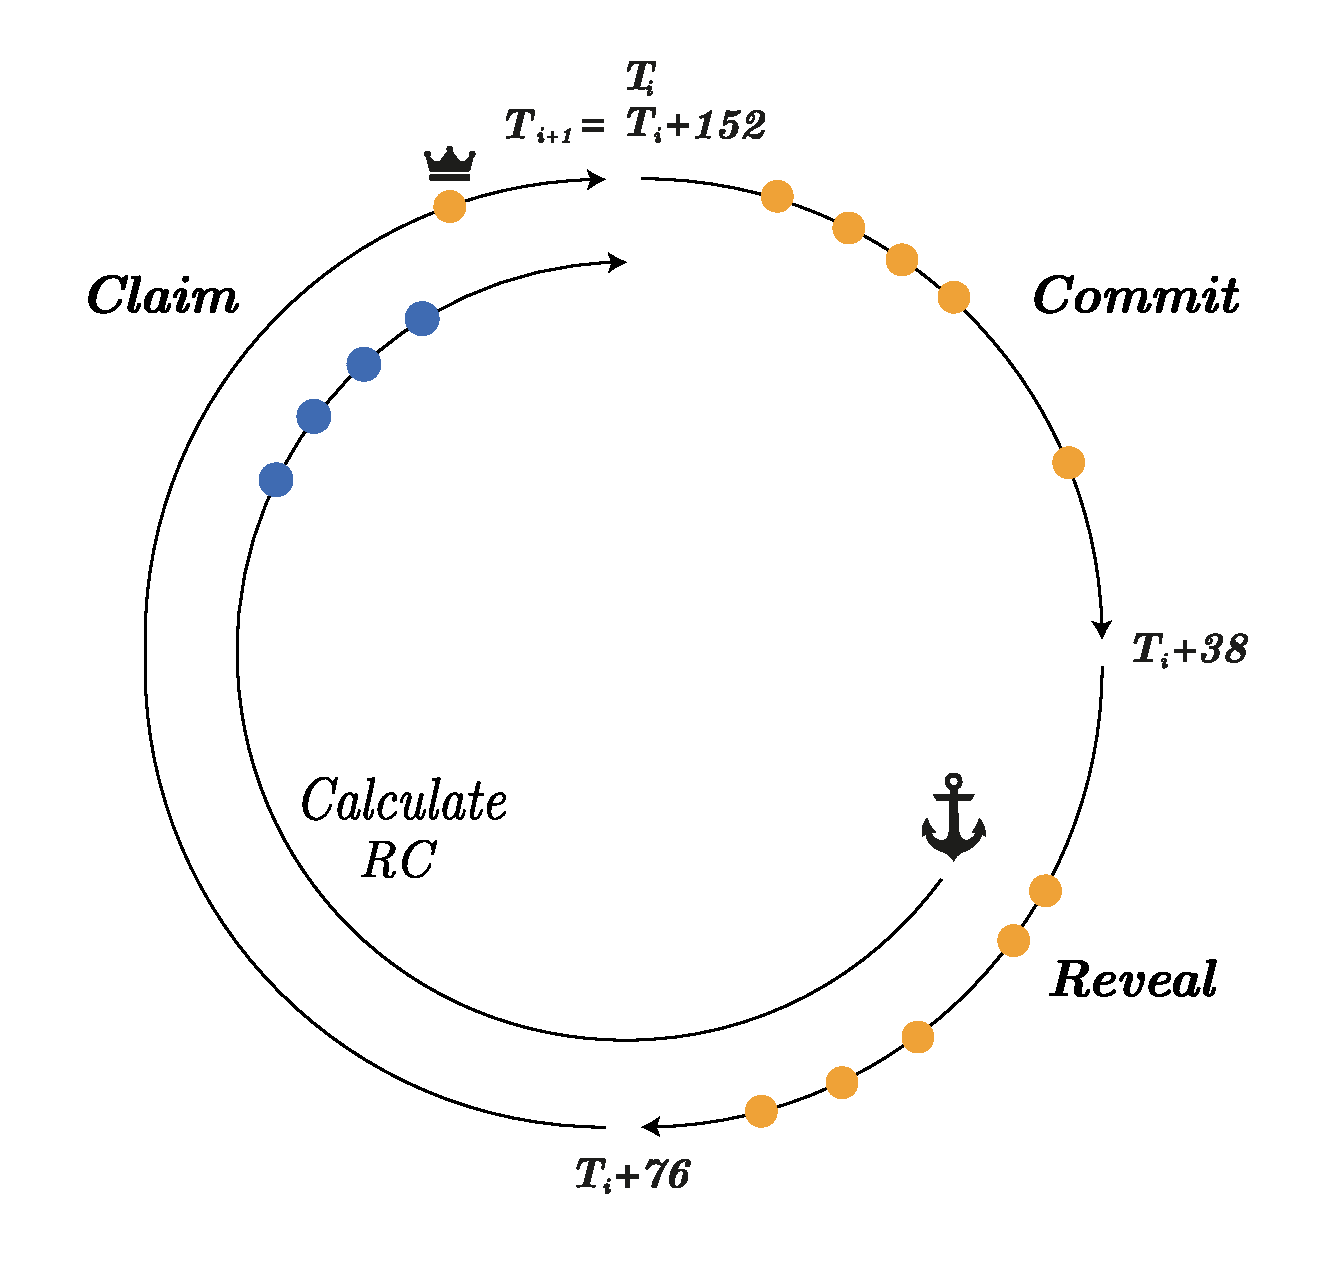
\includegraphics[width=.5\textwidth]{fig/round-lifecycle.pdf}
  \caption[Phases of a round of the redistribution game]{Phases of a round of the redistribution game. The figure displays the timeline of the repeating rounds of the redistribution game with its phases. In the context of smart contract interaction, logically starting with the commit phase, followed by reveal and claim. From the point of view of client node engagement starting with the end of the reveal phase with the neighbourhood selection anchor revealed, those in the selected neighbourhood start calculating their reserve sample only to submit it by the end of the next commit phase. If they are selected as an honest node and as a winner, they submit their proof of entitlement in a claim transaction.}
\label{fig:phases}
\end{figure}    

Once the reveal phase is over, the  \gloss{neighbourhood selection anchor} becomes known. Nodes that have the anchor within their neighbourhood%
%
\footnote{If storage depth is less than the anchor's proximity order relative to the overlay address.}
%
are  allowed to participate in the following round (see figure \ref{fig:neighbourhood-selection}).



The storer nodes in a neighbourhood are assumed to have  consensus over the chunks that make up their reserve and provide evidence called \gloss{proof of entitlement} to the blockchain (discussed below in detail in \ref{sec:por}). In such a game, the Nash-optimal strategy for each node is to follow the protocols and coordinate to guarantee that from the same information, all neighbouring peers will arrive at the same proof of entitlement. Since the proof of entitlement needs to be consensual but unstealable,%
%
\footnote{%
Any explicit communication between independent nodes about this reserve before the end of the commit phase constitutes risk in that it may leak the proof to a node not doing storage work. Therefore nodes are incentivised to keep the proof a secret. Making these proofs unstealable helps detect opportunistic peers that pose as storers but do not provide adequate storage.}
%
a commit/reveal scheme must be used.

In the \gloss{commit phase}, nodes in a neighbourhood will apply by submitting the \gloss{reserve commitment} obfuscated with an arbitrary key that they later reveal% 
% (see definition \ref{def:chc} in appendix \ref{sec:appendix-game})%
. The smart contract receiving the commit transaction verifies that the node is staked, i.e., the registry of the staking contract contains an entry for the node's overlay with a stake that is higher than the minimum stake.

In the \gloss{reveal phase}, each node that previously committed to a reserve, now reveal their commitment by submitting a transaction containing
their reserve commitments, their storage depth,
their overlay address, and the key they used to obfuscate  the commit.
When receiving the reveal transaction, the contract  verifies that the revealed data serialised does indeed hash to their commitment. It is also checked if the node belongs to the neighbourhood designated by the neighbourhood selection anchor, i.e., is within the storage depth provided in the reveal.

In the \gloss{claim phase}, the winner node must submit a claim transaction.%
%
\footnote{Every node in the selected neighbourhood needs to perform the corresponding calculations to determine whether or not they are the winner.}
%
First, in order to decide the outcome of the Schelling game, one reveal is selected  from among the reveals submitted during the reveal phase.%
%
\footnote{This is relevant only if the depth and/or the commitment are non-uniform across applicants.}
%
The selected reveal represents the truth; the set of applications agreeing with the selected one represent the \gloss{honest peers} of the neighbourhood, the ones disagreeing are the \gloss{liars}, while those committers that did not reveal or revealed invalid data are the \gloss{saboteurs}. Honesty is incentivised by the fact that liars and saboteurs get punished. In what follows we introduce staking that is needed for both the selection processes and the punitive measure.


\subsection{Staking}\label{sec:staking}

\subsubsection{Neighbours with shared storage}

In order to provide robust protection against accidental node churn, i.e., ensure retrievability of chunks from a neighbourhood in the face of some nodes being offline, the swarm require a number of independent storers in each neighbourhood physically replicating content.
If payout was given to each node that shows proof of entitlement, then operators would be incentivised to create spurious nodes with the sole purpose of applying for the reward. Measures can be introduced to enforce that these spurious nodes must be operating on the network, but ultimately, operators may choose to actually run several nodes yet share their storage on a single hardware. 
The incentive system must ensure that storage providers do not  adopt this strategy. To this end, we introduce \gloss{staking}.  

Stakes are used as weights by the contract to determine the true reserve commitment (truth selection) as well as the winner among the honest nodes (winner selection). Since peers' relative stake determine their chance of winning, stake is additive, i.e., operators' profit only depends on their total stake within the neighbourhood. Given the cost of running a node, operators will have no  motivation to divide their stake between multiple nodes sharing storage hardware.



\subsubsection{Committed stake and stake balance}

When registering in the staking contract, stakers commit to a stake denominated in rent units called 
\gloss{committed stake}.  The committed stake must have a lower bound.%
%
\footnote{A large number of staked nodes could cause the claim transaction to fail due to gas cost needed for iterating over them. This presents a potential attack where the adversary registers stakes for many nodes and commits for all of them. Such an attack is made prohibitively costly by enforcing a minimum stake.}
%
The  amount sent with the transaction is recorded and serves as collateral called \gloss{stake balance}. Stakes can be created or topped up any time, but the update time is recorded together with the amount.
Participation is restricted to peers whose stake has not changed recently, thereby excluding the possibility of changing stakes after knowing the selected neighbourhood.
Every time the stake of a node is queried, the contract returns  the  absolute committed stake in BZZ calculated as (1) the committed stake in rent units multiplied by the unit price of rent  or (2) the entire stake balance, whichever is smaller%
% (see definition \ref{def:stakes} in appendix \ref{sec:appendix-game})
.  

Stakes must be transferable between overlay addresses to facilitate neighbourhood hopping in case the distribution of stake per neighbourhood is unbalanced. 

\subsubsection{Withdrawability of surplus stake balance}



The committed stake lets operators express their  profit margin together with time preference for realising this profit. Since the profit is only transparent once the relative stakes within the neighbourhood are known, it is possible that nodes take a while to discover their optimal stake. 

If the BZZ token price increases and the unit price of rent drops, the entry for the node in the stake registry will show excess balance. This surplus can always be withdrawn,
and, as a consequence, stakers can realise their profit from BZZ appreciation.%
%
\footnote{In case the token price goes up substantially, the stake balance ends up worth much more than what nodes can ever expect to earn. If the stake balance was not at all withdrawable, participation would be disincentivised due to fear of losing the potential gains in the event of BZZ token appreciation.}
% 

 
%%%%%%%%%%%%%%%%%%%%%%%%%%%%%%%%%%%
\subsection{Neighbourhood consensus over the reserve}\label{sec:por}

Peers applying for the round must agree on which chunks belong to their respective reserves. For this, at the very least, the applicants must consent on their area of responsibility, which can be derived from their storage depth and their overlay address.  
The consensus over the reserve content is tested with the identity of a \gloss{reserve sample}.
The sample is the first $k$ chunks in the reserve using an ordering based on a modified hash of the chunks%
% (see \ref{def:transformed-reserve} in appendix \ref{sec:appendix-game})
.  The modified chunk hash is  obtained using the chunk contents and a \emph{salt} specific to the round.%
%
\footnote{This modified hash is the BMT hash of the chunk data using Keccak-256 prefixed with the reserve sample salt as a base hash%
% (defined in \ref{def:prefixed-hash} in appendix \ref{sec:appendix-game})
. The ordering is the ascending integer order reading the 32-byte modified hash as a big-endian encoded 256-bit integer%
% (see \ref{def:sampler} in appendix \ref{sec:appendix-game})
.}
%
It is impossible for any node to construct this set unless they store all (or a substantial number of the) valid chunks together with their data at or after the time the salt is revealed. 

\subsubsection{Recency and sampling}

The reserve sample must exclude too recent chunks because, otherwise, malicious uploaders could bombard nodes in the neighbourhood with a non-identical set of chunks  that are going to be sampled thereby breaking the consensus about the reserve. One way to guard against this attack is to save each chunk together with its time of storage%
%
\footnote{Using the timestamp within the postage stamp to define the minimum age on would not solve the consensus problem since chunks with old postage stamp could be circulated towards the end of sampling and cause disagreement between neighbours.}
% 
in the local database.
Pairwise synchronisation of chunks between neighbours with the pull-sync protocol respects this ordering by time of storage. 
We require that live syncing, i.e., syncing of chunks received after the peer connection started has a latency not longer than an agreed constant duration called \gloss{maximum syncing latency} (or \emph{max sync lag} for short). Peer connections lagging more with syncing are by protocol not counted as legit storer nodes. This restriction ensures that malicious nodes can not back-date new chunks more than the max sync lag without losing their storer status. 

In order to reach consensus, we must ensure that all chunks received by any node in the neighbourhood not later than $l$ should reach every node of the neighbourhood before the claim phase.
% This means that after receiving the chunk with a lag, the client still has time to include it in their sample and safely submit the commit transaction.
%
If we choose $l$ as 2 times the allowed sync lag then every chunk landing first with a node has time to arrive at each node to be safely included in a consensual sample.%
%
\footnote{Instead of actually monitoring neighbour connections and abstain from committing to a sample in case of excessive lag, one can just choose a small enough sample size.}%
%

\subsubsection{Storage depth and honest neighbourhood size}

In order to decide which reveal represents the truth for the current round, one submission out of all reveals is selected randomly with a probability proportional to the amount of stake the revealer has. More precisely: the amount of stake per neighbourhood size, i.e.,    \gloss{stake density}. The reserve sample hash and the reported storage depth thus revealed are considered the truth for the current round. 

Now we can understand why nodes will report actual storage depth correctly. If a node chooses to play with a larger neighbourhood than the neighbours, it will be selected more often than the others. However, as the committed storage depth decreases as compared to peers, the node's stake is counted with an exponentially deflated  value relative to the peers reporting a deeper storage radius, making such an attack costly.  

Overreporting storage depth is possible as long as the the node falls into this narrower proximity of the neighbourhood selection anchor. Therefore, a systematic exploit requires the malicious actor to control a staked node in each subneighbourhood of the true honest neighbourhood. 
On top of this, the winners also need to show evidence that the set of chunks within their storage depth do fill their reserve. 
The actual integer values of the transformed chunk addresses in the sample hold information regarding the size of the original sampled set.  
Requiring the size of the sampled set to fall within the expected range (with sufficient certainty) translates to imposing a constraint on the upper bound of the values of the sample. This construct is called \gloss{proof of density}% 
% (see definition \ref{def:chunk-density-validition} and appendix \ref{sec:density})%
.
%

Note that the sample-based density proof can be spoofed if the attacker is mining content filtering chunks in such a way that the transformed chunk addresses form a dense enough sample, then uses its own postage batches to stamp them. 
Further hardening against such attacks can be achieved by requiring  additionally a commitment to the entire set of postage stamps and similarly proving from a randomised sample the custody of a sufficient quantity. Due to this requirement, fraudulent claimants must not only generate the content, but must also have enough storage slots to fake the sample. This would require the attacker to purchase postage batches in the magnitude of the entire network 
or keep track of and store the actual postage stamps existing in the network. The former imposes a prohibitive cost on the attacker, whereas, in the latter case, the malicious claimant must bear the risk of relying on honest  neighbours for the post-hoc retrieval of witness chunk data needed for the proof of entitlement.
% See figure \ref{fig:proof-of-density}

% \begin{figure}[!ht]
%   \centering
%     % \includegraphics[width=\textwidth]{fig/rproof-of-density.pdf}
%   \caption[Proof of density]{Proof of density.}
% \label{fig:proof-of-density}
% \end{figure}    


\subsubsection{Skipped rounds and rollover}

If there is no claim in a given round, the pot simply rolls over and increase the outpayment for the next round of the redistribution. This policy is by far the easiest to implement, resulting in the lowest gas expenditures.% 
%
\footnote{One might argue for reimbursing honest nodes for their transaction costs. Thereby,  nodes with really small stakes can still participate and in general nodes are less exposed to variance in the probabilistic outpayments.}

\subsubsection{The eight rules of entitlement}

Here we summarise the eight rules of validating a claim (with committing and revealing a reserve commitment and then submitted evidence as proof of entitlement; see also table~\ref{tab:gr8}):%
%
% \footnote{The first three criteria are part of the conditions for staking, committing, and revealing (see definitions \ref{def:chc} and \ref{def:chs} for replication, \ref{def:stakes} and \ref{def:commits} for redundancy, \ref{def:reveals} for responsibility in appendix \ref{sec:appendix-game}. Relevance, retention, recency and  retrievability are proved as part of the proof of reserve (definition \ref{def:por}) and validated as part of the claim (\ref{def:por-validation}). Finally, proof of resources involves density proofs for chunks and stamps (definitions \ref{def:chc} and \ref{def:chs}) validated as part of the claim (definitions \ref{def:chunk-density-validition} and \ref{def:stamp-density-validition}, respectively). The specific construct of proof of entitlement is defined in \ref{def:poe} and its validation in \ref{def:claim-validation} in appendix \ref{sec:appendix-game}).}
%
\begin{itemize}[noitemsep]
%
\item[\hbox to 2em{\textsc{replication}}] \hspace{1cm}\\ Since liars get frozen (i.e., nodes that had revealed reserve commitment hash or storage depth different  from the winner are excluded from the game for a period), nodes in a neighbourhood are incentivised to replicate their reserve by syncronising the chunks they store using the pull-sync protocol.
%
\item[\hbox to 2em{\textsc{redundancy}}] \hspace{1cm}\\ The stake is used as weights in determining the within-neighbourhood probability of a node being selected as winner%
% (see \ref{def:winner-selection})%
. This implies no benefit in submitting multiple claims. Operators running multiple nodes in one neighbourhood (sharing storage) therefore have no advantage over running a single node with the same total stake. Assuming this disincentive to proliferate is effective, staking can be regarded as guarantee for true redundancy.
%
\item[\hbox to 2em{\textsc{responsibility}}] \hspace{1cm}\\  At the time of revealing it is checked if the neighbourhood selection anchor falls within the node's radius of responsibility, i.e., belong to the covered range of addresses whose proximity to the node's overlay address is not less than their reported storage depth. 
%
\item[\hbox to 2em{\textsc{relevance}}] \hspace{1cm}\\ Using a witness proof with the reserve commitment hash as root, we show evidence that an arbitrarily chosen segment in the reserve sample packed address chunk is the address of a witness chunk. 
A valid postage stamp signed off on this witness chunk address is presented to show that storing that chunk  in the reserve is relevant to someone (and is paid for). 
\item[\hbox to 2em{\textsc{retention}}] \hspace{1cm}\\ A segment inclusion proof is provided as evidence that the chunk data has been retained in full integrity. 
\item[\hbox to 2em{\textsc{recency}}] \hspace{1cm}\\ The salt used for the transformed reserve sample is derived from the current round's random nonce proving that the RS must have been compiled recently. The witness and segment indexes are derived from the next game's random seed ensuring that at the time of compilation and commitment, no compressed or partial retention of chunk data would have been
sufficient.
\item[\hbox to 2em{\textsc{retrievability}}] \hspace{1cm}\\  The chunk is shown to be retrievable by proximity based routing, i.e. its address belongs to the range of addresses covered by the neighbourhood: the chunk's proximity order to the node's overlay address is not less than their reported storage depth. 
\item[\hbox to 2em{\textsc{resources}}] \hspace{1cm}\\ Resource retention checks the volume of resources constituting the reserve by estimating the sampled set size via chunks density and stamps density. 
\end{itemize}


{\small \begin{longtable}{l|p{.4\textwidth}|p{.4\textwidth}}
\toprule
 {proof of} & {construct used} & {attacks mitigated}\\\midrule
 \textsc{replication}& Shelling-game over reserve sample& non-syncing, laggy syncing\\
 \textsc{redundancy}& share of reward proportional to stake & shared storage, over-application\\
 \textsc{responsibility}& proximity to anchor & depth/neighbourhood misreporting \\
 \textsc{relevance}& scarcity of postage stamps & generated data \\
 \textsc{retention}& segment inclusion proof & non-storage, partial storage\\
 \textsc{recency}& round-specific salt for reserve sample & create proof once and forget data\\
 \textsc{retrievability}& proximity of chunk & depth over-reporting\\ 
 \textsc{resources}& density-based reserve size estimation & targeted chunk generation (mining) \\\bottomrule
  \caption[r8: proofs used as evidence for entitlement to reward]{r8: proofs used as evidence for entitlement to reward.}
\label{tab:gr8}
 \end{longtable}
 }


\subsection{Pricing and network dynamics}\label{sec:price-oracle}

In this section, we first put the redistribution scheme in the context of self-sustainability, and provide a simple solution for price discovery.

For Swarm to be a truly self-sustaining system, the unit price of storage rent must be set in a way that is responsive to demand and supply. Ideally, the price is automatically adjusted based on reliable signals resulting in dynamic self-regulation. The guiding insight here is that the information storer nodes provide when  they apply for the redistribution game, also serves as a price signal. In other words, the redistribution game serves as a decentralised price oracle.



\subsubsection{Splitting and merging of neighbourhoods}

The storage depth represents the proximity radius within which the neighbourhood's storer nodes keep all chunks with valid postage stamps and fill their reserve. 


If the volume of newly issued storage slots from recently purchased batches (\emph{ingress rate}\/) and the volume of expired storage slots (\emph{outgress rate}\/) balance out, the storage depth remains unchanged.
But see what happens  if the volume of  reserved chunks increase?
Now, since the client's reserve capacity is constant, after a while, nodes are able to fill up their capacity with chunks that are at most one proximity order closer to them than the farthest chunks were previously, i.e.,  their storage depth increases.
When the volume of reserved chunks doubles,  the storage depth increases by one.  

In order to store this excess data under the same redundancy constraints the network requires double the number of nodes. If all else is equal, double the network-wide reserve, double the postage revenue and therefore double the overall pot that gets redistributed. When neighbourhoods split as they are absorbing the new volume, they simultaneously release the chunks in the PO bin of their old depth, i.e., the chunks now stored by their \gloss{sister nodes}. 

Utilisation rate is an organic way to  introduce pressure against fully maxing out a node's reserve with critical content, and thereby enable early detection of capacity pressure. This provides  sufficient safety buffer for the triggered incentives to take effect. For instance,  if utilisation rate is $1/8$, the storage depth is up to 3 PO-s shallower than the reserve depth.%
%
\footnote{The narrative of this scenario is that uploaders with underutilised batches subsidise extra redundancy for everyone.}
%
Now the ingress can be really high and bring the reserve depth down to storage depth. When the tendency of a closing gap between the potential (reserved) and actual (observed) utilisation of the DISC is detected, any incentive change will have the buffer to take effect without target redundancy being threatened. 

% See figure \ref{fig:pricing-demand}.


% \begin{figure}[!th]
%   \centering
%     % \includegraphics[width=.5\textwidth]{fig/pricing-demand.pdf}
%   \caption[Batch utilisation rate as a price signal]{Batch utilisation rate as a price signal.}
% \label{fig:pricing-demand}
% \end{figure}


\subsubsection{Number of honest nodes as price signal}

Since the storage capacity is maxed out, the ratio of supply and demand is directly seen in the number of honest nodes playing the Schelling game. 

We assume that if nodes are staying in the network for a longer period, their doing so testifies to their profitability. For a stable swarm, neighbourhoods need only 4 (balanced) nodes within as neighbourhood. Assuming equal stake (or more precisely, assuming that relative stake equalises profitability of node operators) if there are $n$ nodes in a neighbourhood, their long term profit is equally shared, this amount is optimised if there are exactly four nodes ($n=4$). This number can be more, since opportunistic operators may start their nodes in a complete neighbourhood in anticipation of a neighbourhood split due to capacity demand. As these nodes stay in, the same long term winnings of the neighbourhood gets distributed among more nodes than optimal.
However, the fact that nodes tolerate this implies that the reward is too much (the price is too high), and the network can tolerate a decreasing price.

On the other hand, if the number of honest revealers is less than the neighbourhood redundancy requirement, it signals capacity shortage and therefore requires the storage rent to increase. 

% See figure \ref{fig:pricing-supply}.

% \begin{figure}[!th]
%   \centering
%     % \includegraphics[width=.5\textwidth]{fig/pricing-supply.pdf}
%   \caption[Price signal for supply of storage capacity] {Price signal for supply of storage capacity.}
% \label{fig:pricing-supply}
% \end{figure}


\subsubsection{Parameterisation of the price oracle}

The rule for updating the price from one round to the next is that the current price is multiplied by a value $m$ which depends on the number of honest revealers in the round%
% (formally defined in appendix \ref{sec:appendix-price-oracle})%
. Mathematically, $p_{t+1} = m p_t$, where $p_t$ is the price in round $t$ (and $p_{t+1}$ is then the price in the following round). We define the multiplier $m$ in terms of the number of honest revealers $r$ and a stability parameter $\sigma$ governing how quickly the price should increase or decrease, all other things equal. 

\begin{figure}[!ht]
  \centering
  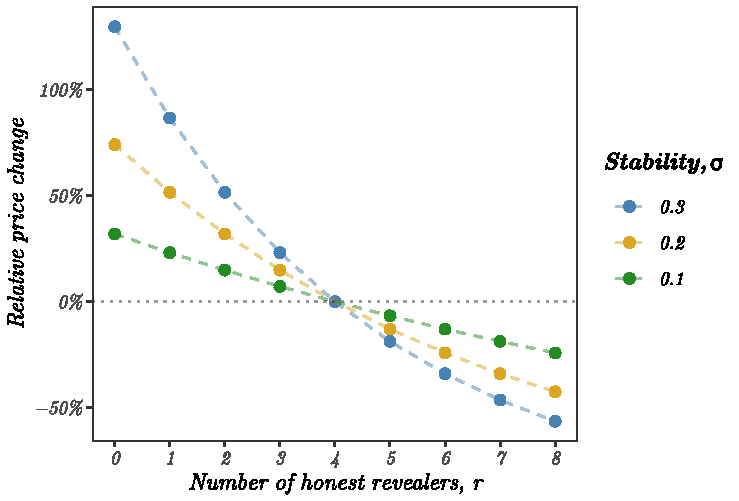
\includegraphics[width=.7\textwidth]{fig/adaptive-pricing.pdf}
  \caption[Adaptive pricing]{Adaptive pricing. The relative change in price (y-axis), mathematically expressed as the price in the next round divided by the price this round minus one ($p_{t+1} / p_t - 1$), is displayed against the number of honest revealers $r$ in the current round (x-axis). This is done so for three different values of the stability parameter $\sigma$ (colours). The points are the actual price change values; the connecting dashed lines are for visual aid only. The dotted horizontal line highlights the point at which no price change happens. Price change is exactly zero for any $\sigma$ when the number of honest revealers is four. Otherwise, larger values of $\sigma$ lead to larger relative price changes as the number of honest revealers is varied.}
  \label{fig:adaptive-pricing}
\end{figure}

In particular, we choose $m = 2^{\sigma(4 - r)}$, and therefore we have $p_{t+1} = 2^{\sigma(4 - r)} p_t$. This expresses how the deviation $4 - r$ of the number of revealers from the optimal value of 4 maps to an exponential change in price. The stability parameter $\sigma$ determines the generic smoothness of price changes across rounds, i.e., how many rounds it takes for the price of rent to double in case of a consistent signal of the lowest degree of undersupply (or halve in case of a consistent oversupply). Figure \ref{fig:adaptive-pricing} illustrates how the price model works.

Two minor adjustments are applied to this simple model. First, $r$ is capped at some value $r_{\text{max}}$ (chosen to be 8 in our case). That is, $r$ should actually be interpreted as the minimum of the number of honest revealers and $r_{\text{max}}$. Second, the price is never allowed to drop below some predetermined minimum $p_{\text{min}}$. That is, in case the price drop from one round to the next would bring the price below $p_{\text{min}}$, it will instead be kept at $p_{\text{min}}$. 




\section{Summary}


In the first two chapters of the architecture part of the book, we introduced the core of Swarm: the peer-to peer-network layer described in Chapter \ref{sec:network} implements a distributed immutable storage for chunks, which is complemented by the incentive system described in the following chapter. The resulting base layer system provides:

\begin{enumerate}[noitemsep]
    \item permissionless participation and access,
    \item zero-cash entry for node operators,
    \item maximum resource utilisation, 
    \item load-balanced distribution of data,
    \item scalability, 
    \item censorship-resistance and privacy for storage and retrieval,
    \item auto-scaling popular content,
    \item basic plausible deniability and confidentiality,
    \item churn-resistance and eventual consistency in a dynamic network with node dropouts,
    \item sustainability without intervention due to built-in economic incentives,
    \item robust private peer-to-peer accounting, 
    \item incentivised bandwidth sharing,
    \item off-chain micro-commitments with on-chain settlement,
    \item DoS resistance and spam protection,
    \item positive (i.e., motivated by reward) incentives for storage,
    \item negative (i.e., discouraged through threat of punitive measures) incentives against data loss.
\end{enumerate}


\chapter{High-level functionality}\label{sec:high-level-functionality}


This chapter builds on the distributed chunk store and introduces data structures and processes that enable higher-level functionality, offering a rich experience handling data. In particular, we show how chunks can be organised to represent files (\ref{sec:files}) and how files can be organised to represent collections (\ref{sec:collections}). We also introduce key--value maps (\ref{sec:maps}) and briefly discuss the potential of arbitrary functional data structures. We then shift our attention to presenting our solution for providing confidentiality and access control (\ref{sec:access-control}). 

In \ref{sec:feeds}, we introduce Swarm feeds, which are designed to represent a wide variety of sequential data, such as versioning updates of mutable resources or indexing messages for real-time data exchange: offering a system of persisted pull messaging. To implement push notifications of all kinds, \ref{sec:pss} introduces the novel concept of \glossplural{Trojan chunk} that allow messages to be disguised as chunks and directed to their intended recipient in the swarm. We explain how Trojan chunks and feeds can be combined to form a fully-fledged communication system with robust privacy features.                                                       

\section{Data structures\statusgreen}\label{sec:datastructures}

\green{}

In the first two chapters, we made the assumption that data is structured in the form of chunks, i.e. fixed-size data blobs. However, in this section, we will present the algorithms and structures that enable the representation of data of arbitrary length. We will introduce \glossplural{Swarm manifest}, which form the basis of representing collections, indexes, and routing tables, allowing Swarm to host websites and offer URL-based addressing.

\subsection{Files and the Swarm hash\statusgreen}\label{sec:files}

In this section, we introduce the concept of the \emph{Swarm hash}, which provides a mechanism for combining chunks to represent larger sets of structured data, such as files. The idea behind the Swarm hashing algorithm is that chunks can be arranged in a Merkle tree. In this structure, leaf nodes correspond to chunks from consecutive segments of input data, while intermediate nodes correspond to chunks that are composed of the chunk references of their children. These combined chunks are packaged together to form another chunk, as illustrated in Figure \ref{fig:Swarm-hash}. 



\begin{figure}[htbp]
\centering
\resizebox{1\textwidth}{!}{
    \input{fig/Swarm-hash.tex}
}
\caption[Swarm hash \statusgreen]{Swarm hash: data input is segmented to 4-kilobyte chunks (gray), that are BMT hashed. Their hashes are packaged into intermediate chunks starting on level $0$, all the way until a single chunk remains on level $n$. }
\label{fig:Swarm-hash}
\end{figure}

\subsubsection{Branching factor and reference size}

The branching factor of the tree is calculated as the chunk size divided by the reference size. For unencrypted content, the chunk reference is simply the \gloss{BMT hash} of the chunk, which is 32 bytes, so the branching factor is just 4096/32 =  128. A group of chunks referenced under an intermediate node is referred to as a \gloss{batch}. If the content is encrypted, the chunk reference consists of the concatenation of the chunk hash and the decryption key. Both are 32 bytes long, so an encrypted chunk reference will be 64 bytes, and therefore the branching factor is 64. 


\begin{figure}[htbp]
\centering
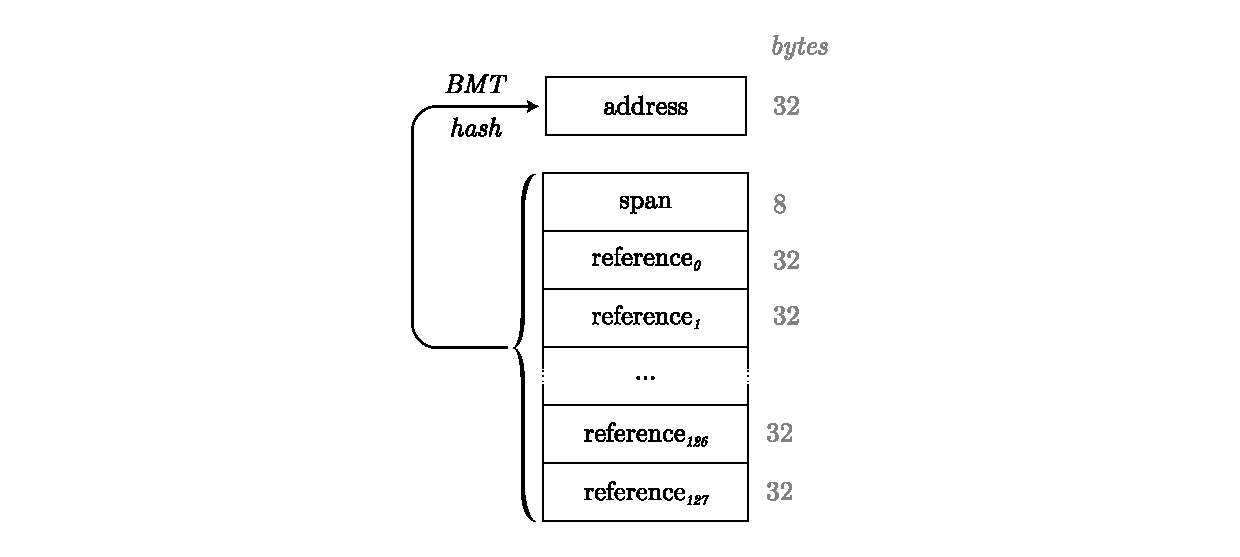
\includegraphics[width=\textwidth]{fig/intermediate-chunk-3.pdf}
\caption[Intermediate chunk \statusgreen]{Intermediate chunk. It encapsulates references to its children.}
\label{fig:intermediate-chunk}
\end{figure}

As a result, a single chunk can represent an intermediate node in the Swarm hash tree, in which case its content can be segmented to references, allowing retrieval of their children. These child nodes themselves may be intermediate chunks, as illustrated in Figure \ref{fig:intermediate-chunk}. By recursively unpacking these from the root chunk downwards, we can eventually obtain a sequence of data chunks. 

 \subsubsection{Chunk span and integrity of depth}

The length of data subsumed under an intermediate chunk is called the \gloss{chunk span}. In order to be able to tell if a chunk is a data chunk or not, the chunk span is prepended to the chunk data in a 64-bit little-endian binary representation. When calculating the BMT hash of a chunk, this span constitutes the metadata that needs to be added to the BMT root and hashed together, resulting in the chunk address. When assembling a file starting from a hash, it is possible to tell if a chunk is a data chunk or an intermediate chunk simply by looking at the span. If the span is larger than 4K, the chunk is an intermediate chunk and its content needs to be interpreted as a series of hashes of its children; otherwise it is a data chunk.

In theory, if the length of the file is already known, spans of intermediate chunks are unnecessary since we could calculate the number of intermediate levels required for the tree. However, using spans disallows reinstating the intermediate levels as data layers. In this way, we impose \emph{integrity of the depth}. 

\subsubsection{Appending and resuming aborted uploads}

The Swarm hash has the interesting property that any data span corresponding to an intermediate chunk is also a file and can therefore be referenced as if the intermediate chunk was its root hash. This property is significant because it enables appending to a file while retaining a historical reference to the earlier state, without duplicating chunks, except for the incomplete right edge of the Merkle tree. Appending data to a file is particularly useful for scenarios such as resuming uploads after a crash partway through uploading big files.

\subsubsection{Random access}

Note that all chunks in a file, except for the right edge, are completely filled. Given that chunks have a fixed size, it is possible to calculate the path to a specific chunk and the offset to search within that chunk for any arbitrary data offset ahead of time. Because of this, \emph{random access to files} is supported right away (see Figure \ref{fig:random-access}).


\begin{figure}[htbp]
\centering
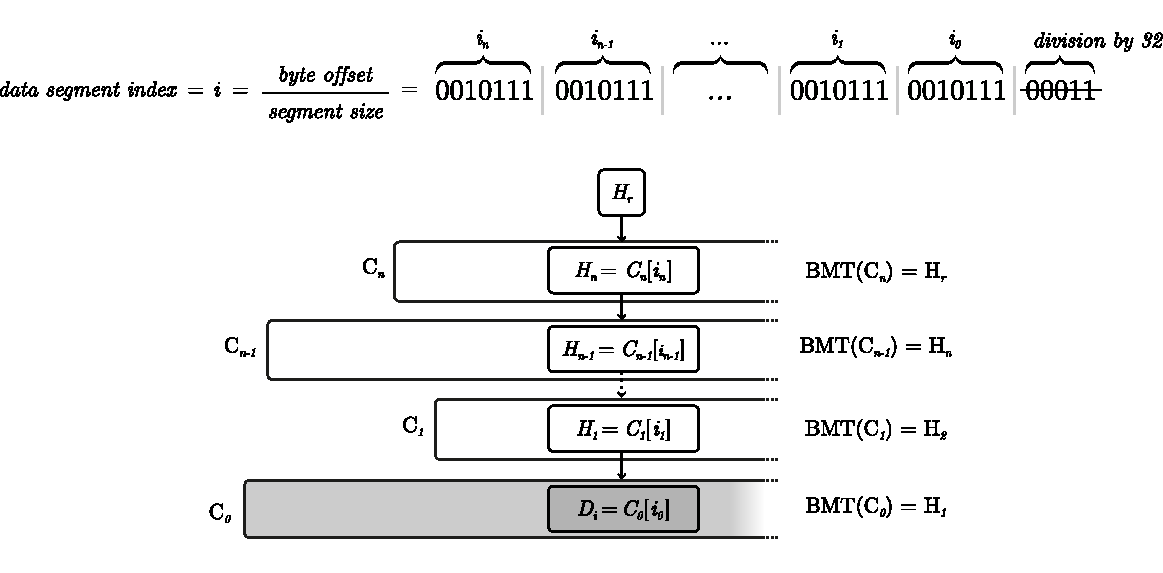
\includegraphics[width=\textwidth]{fig/random-access.pdf}
\caption[Random access at arbitrary offset with Swarm hash \statusgreen]{Random access at arbitrary offset with Swarm hash. The arbitrary offset informs us how to traverse the Swarm hash tree.}
\label{fig:random-access}
\end{figure}

\subsubsection{Compact inclusion proofs for files}


\begin{figure}[htbp]
\centering
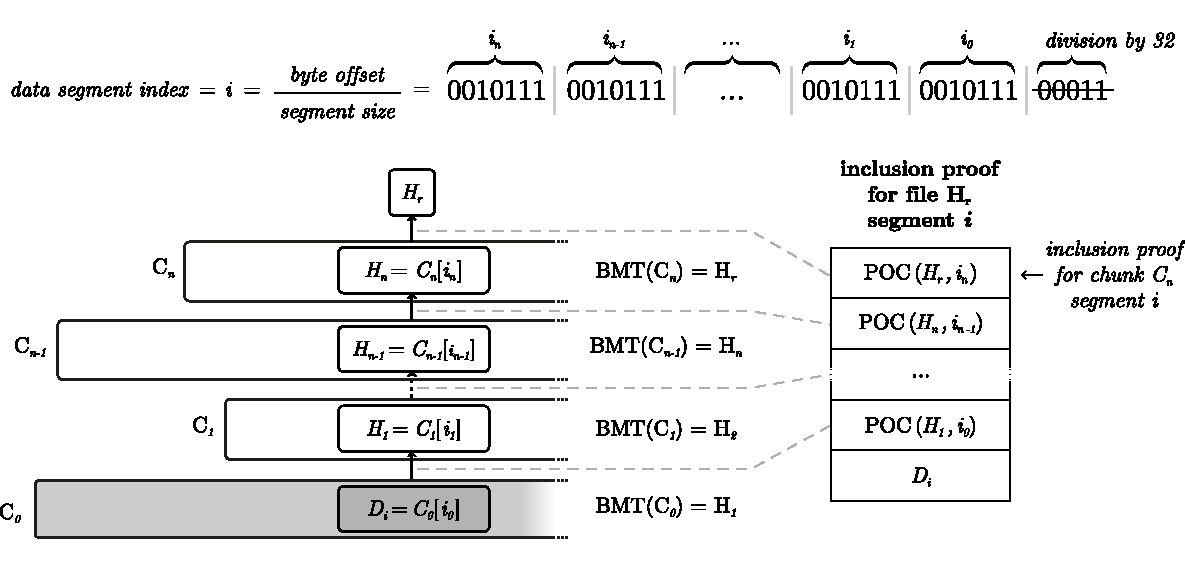
\includegraphics[width=\textwidth]{fig/file-inclusion.pdf}
\caption[Compact inclusion proofs for files \statusgreen]{Compact inclusion proofs for files. If we need to prove inclusion of segment   $i$, after division by 32 (within-segment position), we follow groups of 7 bits to find the respective segment of the intermediate node.}
\label{fig:file-inclusion}
\end{figure}


Suppose we were to prove the inclusion of a substring in a file at a particular offset. We have observed that the offset, when applied to the data, follows a deterministic path traversing the Swarm hash. Since a substring inclusion proof simply reduces to a series of proofs of data segment paths, the chunk addresses are a result of a BMT hash, where the base segments are 32 bytes long. This means that in intermediate chunks, BMT base segments align with the addresses of their children. As a consequence, proving that a child of an intermediate chunk at a particular span offset is equivalent to giving a segment inclusion proof on the child hash. Therefore, substring inclusion in files can be proved with a sequence of BMT inclusion proofs where the length of the sequence corresponds to the depth of the Swarm hash tree (see Figure \ref{fig:file-inclusion}). 


Note that such inclusion proofs are possible even in the case of encrypted data. This is because the decryption key for a segment position can be selectively disclosed without revealing any information that could compromise the encryption of other parts in the chunk.

In this section, we have presented the Swarm hash, a data structure over chunks that represents files, which supports the following functionalities:

\begin{itemize}[noitemsep]
    \item \emph{random access} -- The file can be read from any arbitrary offset with no extra cost.
    \item \emph{append} -- Supports appending without duplication. 
    \item \emph{length-preserving edits} -- Supports length-preserving edits without the duplication of unmodified parts.
    \item \emph{compact inclusion proofs} -- Allow inclusion proofs with resolution of 32 bytes in space logarithmic in file size.
\end{itemize}



\subsection{Collections and manifests\statusgreen}\label{sec:collections}

The \gloss{Swarm manifest} serves as a framework that defines a mapping between arbitrary paths and files to represent collections. It includes metadata associated with the collection and its objects (files). A \gloss{manifest entry} contains a reference to a file or, more precisely, a reference to the Swarm root chunk of the representation of file (see \ref{sec:files}) and also specifies the media mime type of the file to ensure that browsers can appropriately handle it. A manifest can be thought of as (1) a routing table, (2) a directory tree, or  (3) an index, which makes it possible for Swarm to implement (1) web sites, (2) file-system directories, or (3) key--value stores (see \ref{sec:maps}), respectively. The use of manifests is essential for URL-based addressing within Swarm (see \ref{sec:urls}). 

Manifests are represented as a compacted trie%
%
\footnote{See \url{https://en.wikipedia.org/wiki/Trie}}
%
in which individual trie nodes are serialised as chunks. The paths are associated with a \gloss{manifest entry} that specifies at least the \emph{reference}. The reference may point to an embedded manifest if the path is a common prefix of more than one path in the collection, thereby implementing branching in the trie, as depicted in Figure \ref{fig:manifest-structure}. 


\begin{figure}[htbp]
\centering
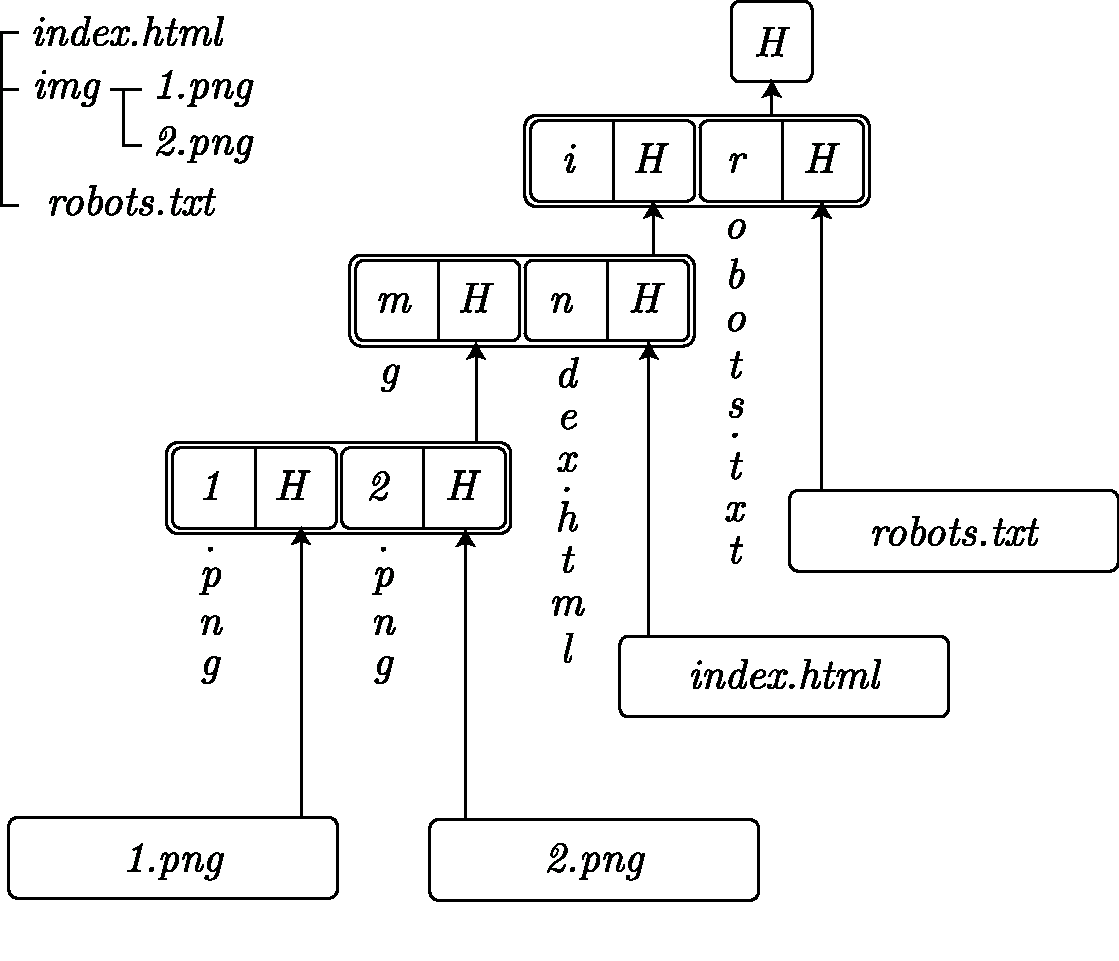
\includegraphics[width=0.7\textwidth]{fig/manifest-structure.pdf}
\caption[Manifest structure \statusgreen]{Manifest structure. Nodes represent a generic trie node: it contains the forks which describe continuations sharing a prefix. Forks are indexed by the next byte of the key, whose value contains the Swarm reference to the child node as well as the longest prefix (compaction).}
\label{fig:manifest-structure}
\end{figure}

\begin{figure}[htbp]
\centering
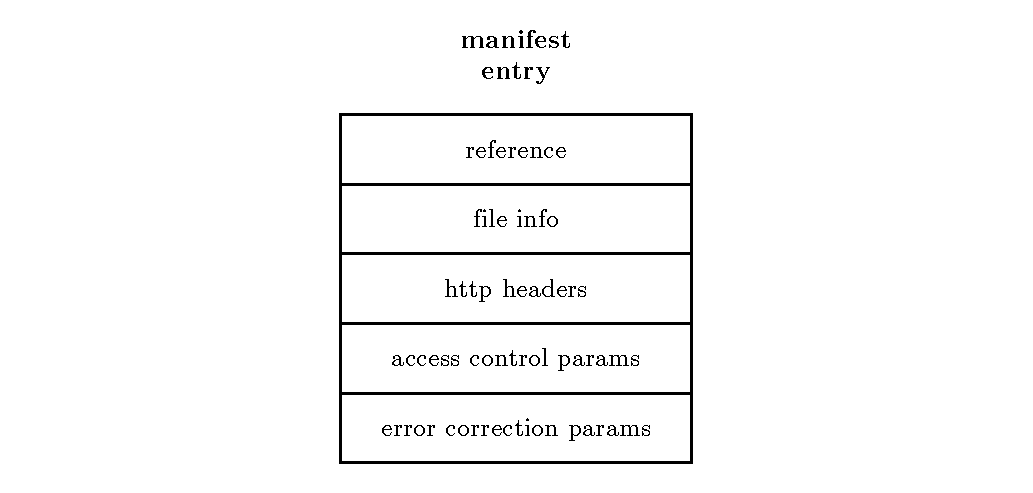
\includegraphics[width=\textwidth]{fig/manifest-entry.pdf}
\caption[Manifest entry \statusgreen]{Manifest entry is a data  structure that contains the reference to a file including metadata about a file or directory  pertaining to the assembler, access control, and http headers.}
\label{fig:manifest-entry}
\end{figure}

A manifest entry is essentially a reference that provides information about a file or directory.
The metadata pertains to the following areas of concern: 

\begin{itemize}
  \item Parameters for the downloader component, responsible for assembling chunks into a byte stream. This includes access control information, erasure coding parameters, and the publisher needed for chunk recovery.
  
  \item Information relevant to client-side rendering, handled by the browser. This may include content type headers, or generically HTTP headers, that are picked up by the local swarm client's API and set in the response header when the file is retrieved.
  
  \item File information mapped to the file system during downloading, such as file permissions.
\end{itemize}

The high-level API for manifests offers functionality for uploading and downloading files and directories. It also provides an interface for adding documents to a collection on a path and deleting a document from a collection. Note that deletion here only means that a new manifest is created in which the path in question is omitted. There is no other notion of deletion in Swarm, i.e. the referenced value in the deleted manifest entry still remains in Swarm. Swarm exposes the manifest API via the \emph{bzz URL scheme}.

\subsection{URL-based addressing and name resolution\statusgreen}\label{sec:urls}

Earlier, we introduced the low-level network component of Swarm as a distributed immutable store of chunks (DISC, see \ref{sec:disc}). In the previous two sections, we discussed how files (\ref{sec:files}) and collections (\ref{sec:collections}) can be represented in Swarm and identified using chunk references. Manifests provide a way to index individual documents in a collection, enabling them to serve as representations of websites hosted in Swarm. The root manifests serve as the entry-points to virtually hosted sites on Swarm and are therefore analogous to hosting servers. In the current web, domain names resolve to the IP addresses of host servers, and URL paths (of static sites) are mapped to entries in the directory tree based on their path relative to the document root set for the host.
Analogously, in Swarm, domain names resolve to references to the root manifests, and URL paths are mapped to manifest entries based on their path.  

When the HTTP API serves a URL, the following steps are performed:

\begin{enumerate}
    \item \emph{domain name resolution} -- Swarm resolves the host part to a reference to a root manifest,
    \item \emph{manifest traversal} -- recursively traverse embedded manifests along the path matching the URL path to arrive at a manifest entry,
    \item \emph{serving the file} -- the file referenced in the manifest entry is retrieved and rendered in the browser with headers (notably content type) obtained from  the metadata of manifest entry.
\end{enumerate}

Swarm supports domain name resolution using the \gloss{Ethereum Name Service} (\gloss{ENS}). \gloss{ENS} is the system that, analogously to the DNS of the old web, translates human-readable names into system-specific identifiers, i.e., references in the case of Swarm.
%
In order to use ENS, a Swarm node needs to be connected to an EVM-based blockchain that supports the Ethereum API (ETH mainnet, Ropsten, ETC, etc). 
Users of ENS can register a domain name on the blockchain and set it to resolve to a reference, most commonly the content hash of a public (unencrypted) manifest root. In the case that this manifest represents a directory containing the assets of a website, the default path for the hash may be set to be the desired root HTML page. When an ENS name is navigated to using a Swarm-enabled browser or gateway, Swarm will simply render the root HTML page and serve the rest of the assets provided in the relative path. Swarm facilitates easy website hosting, while also providing an interface to older pre-existing browsers and offering a decentralised improvement over the traditional DNS system.


\subsection{Maps and key--value stores\statusgreen}\label{sec:maps}

This section describes two methods for implementing a simple distributed key--value store in Swarm. Both rely solely on tools and APIs which have been already introduced.

The first technique involves using manifests: Paths represent keys and the reference in the manifest entry with the particular path point to the value. This approach benefits from a full API enabling insert, update and remove through the bzz manifest API. Since manifests are structured as a compacted trie, this key--value store is scalable. Index metadata requires storage logarithmic to the number of key--value pairs. Lookup requires logarithmic bandwidth. The data structure allows for iteration that respects key order. 

Single owner chunks also provide a way to define a key--value store.

The second technique simply posits that the index of the single owner chunk be constructed as a concatenation of the hash of the database name and the key. This structure only provides insert, without update or remove. Both insert and lookup are constant space and bandwidth. However, lookup is not safe against false negatives, i.e., if the chunk that represents the key--value pair is not found, this does not mean it has never been created (e.g. it may have been garbage collected). Thus, the single owner chunk based key--value store is best used as (1) a bounded cache of recomputable values, (2) mapping between representations such as a translation between a Swarm hash and a Keccak256 hash as used in the Ethereum blockchain state trie nodes, or (3) conventional relational links, such as likes, upvotes, and comments on social media posts. 


\section{Access control\statusgreen}\label{sec:access-control}

\green{}

This section first addresses the confidentiality of content using encryption. Encryption becomes especially useful once users are granted the ability to manage others' access to restricted content. This encompasses scenarios such as managing private shared content and granting authorisation for members to access specific areas of a web application. In this way, we provide a robust and simple API to manage access control, something that is traditionally handled through centralised gate-keeping which is subject to frequent and disastrous security breaches.

\subsection{Encryption\statusgreen}\label{sec:encryption}

This section focuses on achieving confidentiality in a distributed public data storage. We explore how to fulfill the natural requirement for many use cases to store private information while ensuring that it remains accessible only to specific authorised parties using Swarm. 

It is clear that the pseudo-confidentiality provided by the server-based access control predominantly used in current web applications is inadequate. In Swarm, nodes are expected to share the chunks with other nodes, in fact, storers of chunks are incentivised to serve them to anyone who requests them. This decentralised architecture makes it infeasible for nodes to act as the gatekeepers trusted with controlling access to the data. Moreover, since any node in the network could potentially be a storer, the confidentiality solution must not reveal any information that could distinguish a private chunk from random data. As a consequence of this, the only way to prevent unauthorized parties from accessing private chunks is through encryption. In Swarm, if a requestor is authorized to access a chunk, they must possess a decryption key that allows them to decrypt the chunk. Unauthorized parties, on the other hand, must not have access to the decryption key. Incidentally, this mechanism also serves as the basis for \gloss{plausible deniability}.

Encryption at the chunk level is described in \ref{sec:chunk-encryption}. It 
has the desirable property of being virtually independent of the chunk store layer, using the exact same underlying infrastructure for storing and retrieving chunks as unencrypted content.
The only difference between accessing private and public data is the presence of a decryption/encryption key in the chunk references and the associated minor cryptographic computational overhead.

%, a constant or linear factor.

The storage API's raw \lstinline{GET} endpoint allows both encrypted and unencrypted chunk references. 
Decryption is triggered if the chunk reference is double size; consisting of the address of the encrypted chunk and a decryption key. Using the address, the encrypted chunk is retrieved, stored, and decrypted using the supplied decryption key. The API responds with the resulting plaintext.

The storage API's \lstinline{POST} endpoint expects users to indicate if they want to have encryption on the upload or not. In both cases, the chunk will be stored and push-synced to the network, but if encryption is desired, the encrypted chunk needs to be created first. If no further context is given, a random encryption key is generated which is used as a seed to generate random padding to fill the chunk up to a complete 4096 bytes if needed, and finally this plaintext is encrypted with the key. In the case of encryption, the API \lstinline{POST} call returns the Swarm reference, which consists of the Swarm hash as the chunk address and the encryption key. 

In order to guarantee the uniqueness of encryption keys as well as to ease the load on the OS's entropy pool, it is recommended (but not required) to generate the key as the \gloss{MAC} of the plaintext using a (semi-) permanent random key stored in memory. 
This key can be permanent and generated using \lstinline{scrypt} \cite{percival2009stronger}
with a password provided upon startup. Instead of the plaintext, a namespace and path of the manifest entry can be used as context.
Using a \gloss{key derivation function} in this way has the consequence that chunk encryption will be deterministic as long as the context is the same: If we exchange one byte of a file and encrypt it with the same context, all data chunks of the file except the one that was modified will end up being encrypted exactly as the original. Encryption is therefore deduplication-friendly. 


\subsection{Managing access\statusgreen}\label{sec:managing-access}

This section describes the process the client needs to follow in order to obtain the full reference to the encrypted content. This protocol relies on basic meta-information, which is simply encoded as plaintext metadata and explicitly included in the root manifest entry for a document. This level of access, known as \gloss{root access}, does not require special privileges.

In contrast, \gloss{granted access} is a type of selective access that necessitates both root access and access credentials, i.e. an authorised private key or passphrase. Granted access allows different levels of privileges for accessing the content by multiple parties sharing the same root access. This approach allows for updating the content without changing access credentials. Granted access is implemented using an additional layer of encryption on references.

The symmetric encryption of the reference is called the \gloss{encrypted reference}, and the symmetric key used in this layer is called the \gloss{access key}.

In the case of granted access, the root access meta-information contains both the encrypted reference and the additional information required for obtaining the access key using the access credentials. Once the access key is obtained, the reference to the content is obtained by decrypting the encrypted reference with the access key. The resulting full reference consists of the address root chunk and the decryption key for the root chunk. The requested data can then be retrieved and decrypted using the standard method.

The access key can be obtained from a variety of sources, three of which we will define.

\begin{figure}[htbp]
\centering
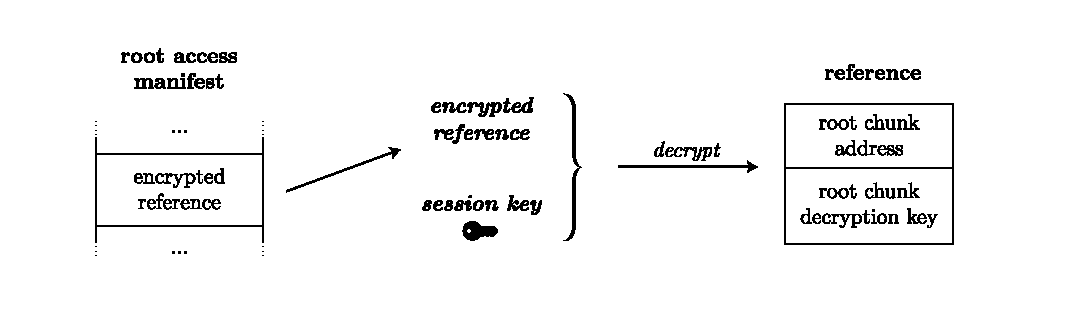
\includegraphics[width=\textwidth]{fig/access-control-single-party.pdf}
\caption[Access key as session key for single party access  \statusyellow]{Access key as session key for single party access.}
\label{fig:access-control-single-party}
\end{figure}

First, a \gloss{session key} is derived from the provided credentials. In the case of granting access to a single party, the session key is used directly as the access key, see Figure \ref{fig:access-control-single-party}. However, in the case of multiple parties, an additional mechanism is used to transform the session key into the access key.

\subsubsection{Passphrase}
The simplest credential is a \emph{passphrase}. The session key is derived from a passphrase using \lstinline{scrypt} with parameters that are specified within the root access meta-information. The output of scrypt is a 32-byte key that may be directly used for Swarm encryption and decryption algorithms.

In typical use cases, the passphrase is distributed by an off-band means with adequate security measures, or exchanged in person. Any user knowing the passphrase from which the key was derived will be able to access the content.

\subsubsection{Asymmetric derivation}

A more sophisticated credential is a \emph{private key}, identical to those used throughout Ethereum for accessing accounts, i.e. an  elliptic curve using secp256k1. In order to obtain the session key, an \gloss{elliptic curve Diffie-Hellman} (\gloss{ECDH}) key agreement must be performed between the content publisher and the grantee. The resulting shared secret is hashed together with a salt. The content publisher's public key as well as the salt are included among metadata in the \gloss{root access manifest}. Based on the standard assumptions of ECDH, this session key can only be computed by the publisher and the grantee and no-one else. 
Once again, when access is granted to a single public key, the session key derived this way can be directly used as the access key for the decryption of the encrypted reference. 
Figure \ref{fig:credentials-to-derive-session-key} summarises the use of credentials to derive the session key.

\begin{figure}[htbp]
\centering
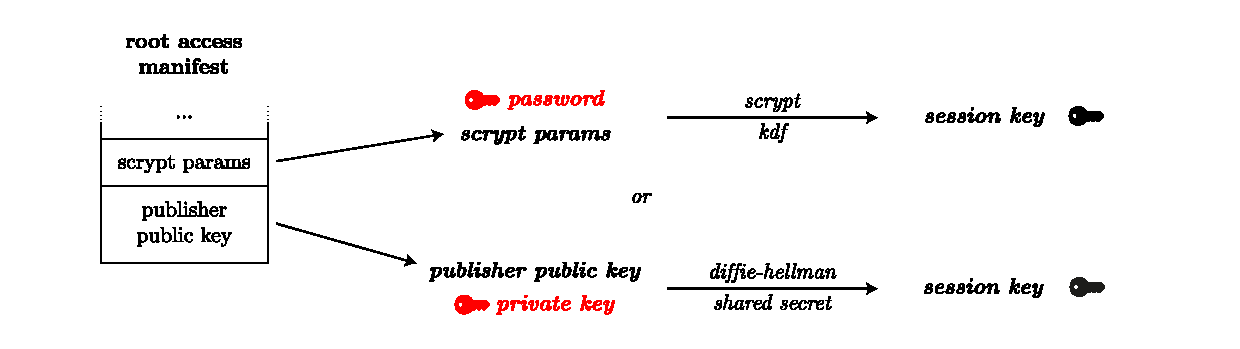
\includegraphics[width=\textwidth]{fig/credentials-to-derive-session-key.pdf}
\caption[Credentials to derive session key  \statusyellow]{Credentials to derive session key.}
\label{fig:credentials-to-derive-session-key}
\end{figure}


\subsection{Selective access to multiple parties\statusgreen}

In order to manage access by multiple parties to the same content, an additional layer is introduced to obtain the access key from the session key. In this variant, grantees can be authenticated using either type of credentials, however, the session key derived as
described above is not used directly as the access key for decrypting the reference. Instead, two keys are derived from the session key: a \gloss{lookup key} and an \gloss{access key decryption key}. These keys are obtained by hashing the session key with two different constants ($0$ and $1$, respectively).

When granting access, the publisher needs to generate a global access key to encrypt the full reference, and then encrypts it with the
access key decryption keys for each grantee. Thereafter, a lookup table is created, mapping each grantee's lookup key to their encrypted access key. Then, for each lookup key, the access key is encrypted with the corresponding access key decryption key.

This lookup table is implemented as an \gloss{access control trie} (\gloss{ACT}) in Swarm manifest format with paths corresponding to lookup keys and manifest entries containing the ciphertext of the encrypted access keys as metadata attribute values. The ACT manifest is an independent resource referenced by a URL, which is included among the root access metadata to indicate whether or not an ACT is to be used.

When accessing content, the user follows these steps: they retrieve the root access meta data, identify the ACT resource, and then calculate their session key using either their passphrase and the scrypt parameters or the publisher public key, their private key, and a salt. From the session key, they can derive the lookup key by hashing it with $0$ and then retrieve the manifest entry from the ACT. For this, they will need to know the root of the ACT manifest and then use the lookup key as the URL path. If the entry exists, the user obtains the value of the access key attribute in the form of a ciphertext that is decrypted with a key derived by hashing the session key with the constant $1$. The resulting access key can then be used to decrypt the encrypted reference included in the root access manifest, see Figure \ref{fig:access-control-multiple-party}. Once the manifest root is unlocked, all references contain the decryption key.

\begin{figure}[htbp]
\centering
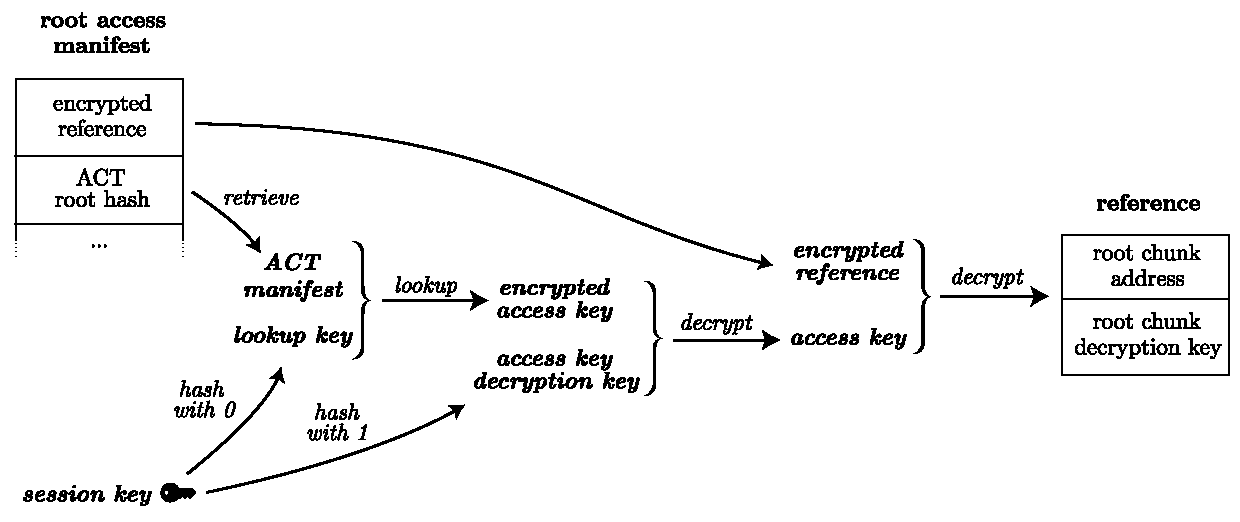
\includegraphics[width=\textwidth]{fig/access-control-multiple-party.pdf}
\caption[Access control for multiple grantees \statusyellow]{Access control for multiple grantees involves an additional layer to get from the session key to the access key. Each user must lookup the global access key specifically encrypted to them. Both the key to look up and the key for decrypting the access key are derived from the session key, which, in turn, requires their credentials.} 
\label{fig:access-control-multiple-party}
\end{figure}


This access control scheme offers several desirable properties:
\begin{itemize}
\item Checking and looking up one's own access is logarithmic in the size of the ACT.
\item The size of the ACT merely provides an upper bound on the number of grantees, without disclosing any information beyond this upper bound about the set of grantees to third parties. Even those included in the ACT can only learn that they are grantees, but obtain no information about other grantees beyond an upper bound on their number.
\item Granting access to an additional key requires extending the ACT by a single entry, which is logarithmic in the size of the ACT. 
\item Revoking access requires changing the access key and therefore the rebuilding of the ACT. Note that this also requires that the publisher retain a record of the public keys of grantees after the initial creation of the ACT.
\end{itemize}

\subsection{Access hierarchy\statusgreen}

In the simplest case, the access key is a symmetric key. However, this represents a special case within a more flexible solution, where
the access key consists of both a symmetric key and a key derivation path derived from a root key. In this case, a derivation path may also be included in addition to the encrypted reference. Any party with an access key whose derivation is a prefix to the derivation path of the reference can decrypt the reference by deriving its key using their own key and the rest of the reference's derivation path.

This allows for a tree-like hierarchy of roles, possibly reflecting an organizational structure. As long as role changes are "promotions", i.e. they result in increased privileges, modifying a single ACT entry for each role change is sufficient.




\section{Feeds: mutability in an immutable store \statusyellow}\label{sec:feeds}

\green{}

Feeds are a unique feature of Swarm that constitute the primary use case for single owner chunks. Feeds can be used for versioning revisions of a mutable resource, indexing sequential updates to a topic, publish parts to streams, or posting consecutive messages in a communication channel, to name but a few. Feeds implement persisted pull-messaging and can also be interpreted as a pub-sub system.

In Section \ref{sec:feed-chunks}, we introduce how feeds are composed of single owner chunks with an indexing scheme, the choice of which we discuss in \ref{sec:indexing-schemes}. We then delve into the importance of feed integrity and methods for verifying and enforcing it in \ref{sec:feed-integrity}. Section \ref{sec:epoch-based-feeds} describes \gloss{epoch-based feeds} which provide feeds that receive sporadic updates a way to be searched. Finally, in \ref{sec:feed-as-channel}, we demonstrate how feeds can be used as an outbox for sending and receiving subsequent messages within a communication channel.


\subsection{Feed chunks \statusyellow}\label{sec:feed-chunks}

A feed chunk is a single owner chunk with the associated constraint that the identifier is composed of the hash of a \gloss{feed topic} and a \gloss{feed index}. The topic is a 32-byte arbitrary byte array, this is typically the Keccak256 hash of one or more human-readable strings specifying the topic and optionally the subtopic of the feed, see Figure \ref{fig:feed-chunk}. 


\begin{figure}[htbp]
\centering
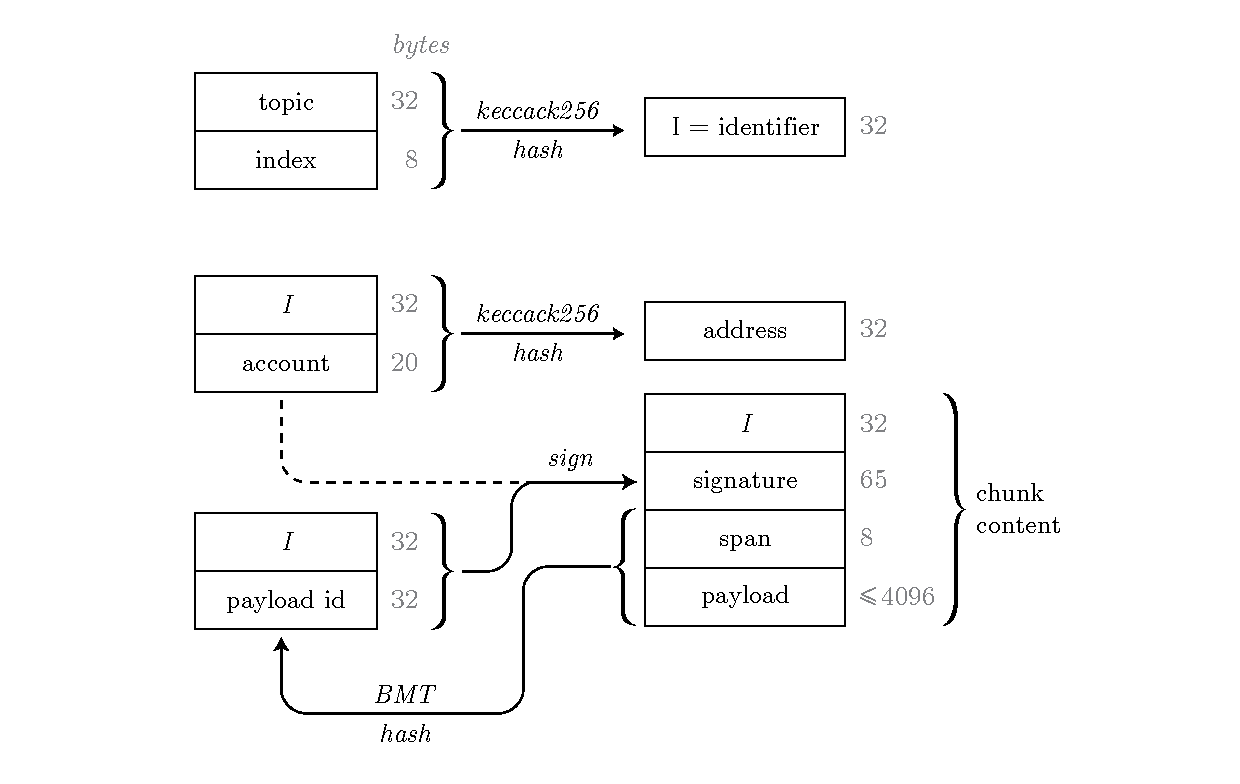
\includegraphics[width=\textwidth]{fig/feed-chunk.pdf}
\caption[Feed chunk \statusgreen]{Feed chunks are single owner chunks where the identifier is the hash of the topic and an index. Indexes are deterministic sequences calculated according to an indexing scheme. Subsequent indexes for the same topic represent identifiers for feed updates.}
\label{fig:feed-chunk}
\end{figure}

The index of a feed can take various forms defining some of the potential types of feeds. The ones discussed in this section are: (1) simple feeds that use incremental integers as their index (\ref{sec:indexing-schemes}); (2)  \gloss{epoch-based feeds} that use an epoch ID (\ref{sec:epoch-based-feeds}); and (3) private channel feeds that use nonces generated through a \gloss{double ratchet} key chain.  (\ref{sec:feed-as-channel}).
The common characteristics among all these feed types is that both the publisher (owner) and the consumer must be aware of the \gloss{indexing scheme}. 

Publishers have exclusive ownership of the feed chunks and are the only ones authorised to post updates to their feed. Posting an update requires (1) constructing the identifier from the topic and the correct index, and (2) signing the identifier concatenated with the hash of the arbitrary content of the update. Since the identifier designates an address in the owner's subspace of addresses, this signature effectively assigns the payload to this address (see \ref{sec:single-owner-chunks}). In this way, all items published on a particular feed can be verified to have been created solely by the owner of the corresponding private key.

On the consumer side, users can retrieve a feed by specifying the chunk address. Retrieving a specific update requires the consumer to construct the address using the owner's public key and the identifier. To calculate the identifier, the user needs two pieces of information: the topic and the appropriate index, for which they need to know the indexing scheme. 

Feeds enable Swarm users to represent a sequence of content updates. The content of each update serves as the payload, which the feed owner signs against the identifier. The payload can be a swarm reference, allowing users to retrieve the associated data.

\subsection{Indexing schemes \statusyellow}\label{sec:indexing-schemes}

Different types of feeds require different \glossplural{indexing scheme} and different lookup strategies. In the following sections, we introduce a few largely independent dimensions in which feeds can be categorised and which appear relevant in making a choice.


The actual indexing scheme used, or even the presence of one (i.e. if the single owner chunk is a feed chunk at all), is left unrevealed in the structure of a feed chunk. As this information is not needed for the validation of a chunk by forwarding nodes, there is no need to include the subtype explicit in the structure. Doing so would only result in unnecessary information leakage. 

\subsubsection{Update semantics}

Updates of a feed can be categorised into three subtypes, each with distinct semantics. 
Revisions, or mutable resource updates are \emph{substitutive}, series updates are \emph{alternative}, while partition updates are \emph{accumulative}. 

Feeds that represent revisions of the same semantic entity are called \gloss{mutable
resource updates}. These resources mutate because the underlying semantic entity changes such as versions of your CV or the resource description becomes more elaborate like the Wikipedia entry about a Roman emperor. Users will typically be interested in the latest update of such resources, with past versions having only historical significance. 

The second subtype, \gloss{series} updates, represents a series of content that is connected by a common thread, theme, or author. Updates in a series are interpreted as alternative and independent instantiations or episodes manifesting in temporal sequence. Examples include social media status updates, a person's blog posts, or blocks of a blockchain.

Finally, there are \gloss{partitions} expressed as feeds, where updates are meant to be accumulated or added to earlier ones. A common example is a video stream consisting of multiple parts. These mainly differ from series in that the individual feed updates are not interpretable on their own, and the temporal sequence may represent a processing order corresponding to some serialisation of the structure of the resource rather than temporal succession. When such a feed is accessed, it may be necessary to accumulate all the parts in order to ensure the integrity of the represented resource.

If subsequent updates of a feed include a reference to a data structure that indexes the previous updates (e.g. a key--value store using the timestamp for the update or simply the root hash of the concatenation of update content), then the \gloss{lookup strategy} in all three cases reduces to retrieving the latest update.

\subsubsection{Update frequency}

Feeds that are updated over time may be categorised into several types. Some are \gloss{sporadic feeds} with irregular asynchronicities, i.e. updates that can have unpredictable gaps. Another type is \gloss{periodic feeds}, where updates are published at regularly recurring intervals.

Additionally, we will discuss \gloss{real-time feeds}, where the update frequencies may not follow a regular pattern but instead vary within the temporal span of real-time human interaction, i.e. they are punctuated by intervals in the second to minute range.

\subsubsection{Subscriptions}

Feeds can be interpreted as \gloss{pub-sub systems} that offer persistence, enabling asynchronous pulls. In what follows, we analyse how the choice of \gloss{indexing scheme} affects the implementation of subscriptions to feeds as pub/sub.

In order to cater for subscribers of a feed, the updates need to be tracked. If we know the latest update, periodic polling needs to be used to fetch subsequent updates. 
If the feed is periodic, one can start polling after a known period. Alternatively, if the feed updates are frequent enough (at most a 1-digit integer orders of magnitude rarer than the desired polling frequency), then polling is also feasible.
However, if the feed is sporadic and updates occur unpredictably, polling may not be practical, and alternative methods such as push notifications (see \ref{sec:trojan} and \ref{sec:notification-requests}) are preferable.

If we have missed out on polling for a period of time due to being offline, or just created the subscription, we can also rely on push notifications or use a \gloss{lookup strategy}. 

Looking up partitions poses no difficulty as each update needs to be fetched and accumulated. In this case, the strategy of just iterating over the successive indexes cannot be improved.
For periodic feeds, we can just calculate the index for a given time, hence asynchronous access is efficient and trivial. 
Looking up the latest version of a sporadically updated feed, however, necessitates some search and hence benefits from \gloss{epoch-based indexing}.



\subsubsection{Aggregate indexing}

A set of sporadic feeds can be turned into a periodic one using \gloss{feed aggregation}. Imagine, for example, a multi-user forum like Reddit, where each registered participant would publish comments on a post using sporadic feeds. In this scenario, it is not practical for each user to monitor the comment feed of every other user and search through their sporadic feeds for updates in order to retrieve all the comments on the thread. It is far more efficient to just do it once though for all users. Indexers do exactly that: aggregate everyone's comments into an index, a data structure whose root can then be published as a periodic feed, see Figure \ref{fig:feed-aggregation}. The period can be chosen to provide a real-time feed experience; even if the rate of change does not justify it, i.e. some updates will be redundant, the cost amortises over all users who use the aggregate feed, making it economically sustainable. 

\begin{figure}[htbp]
\centering
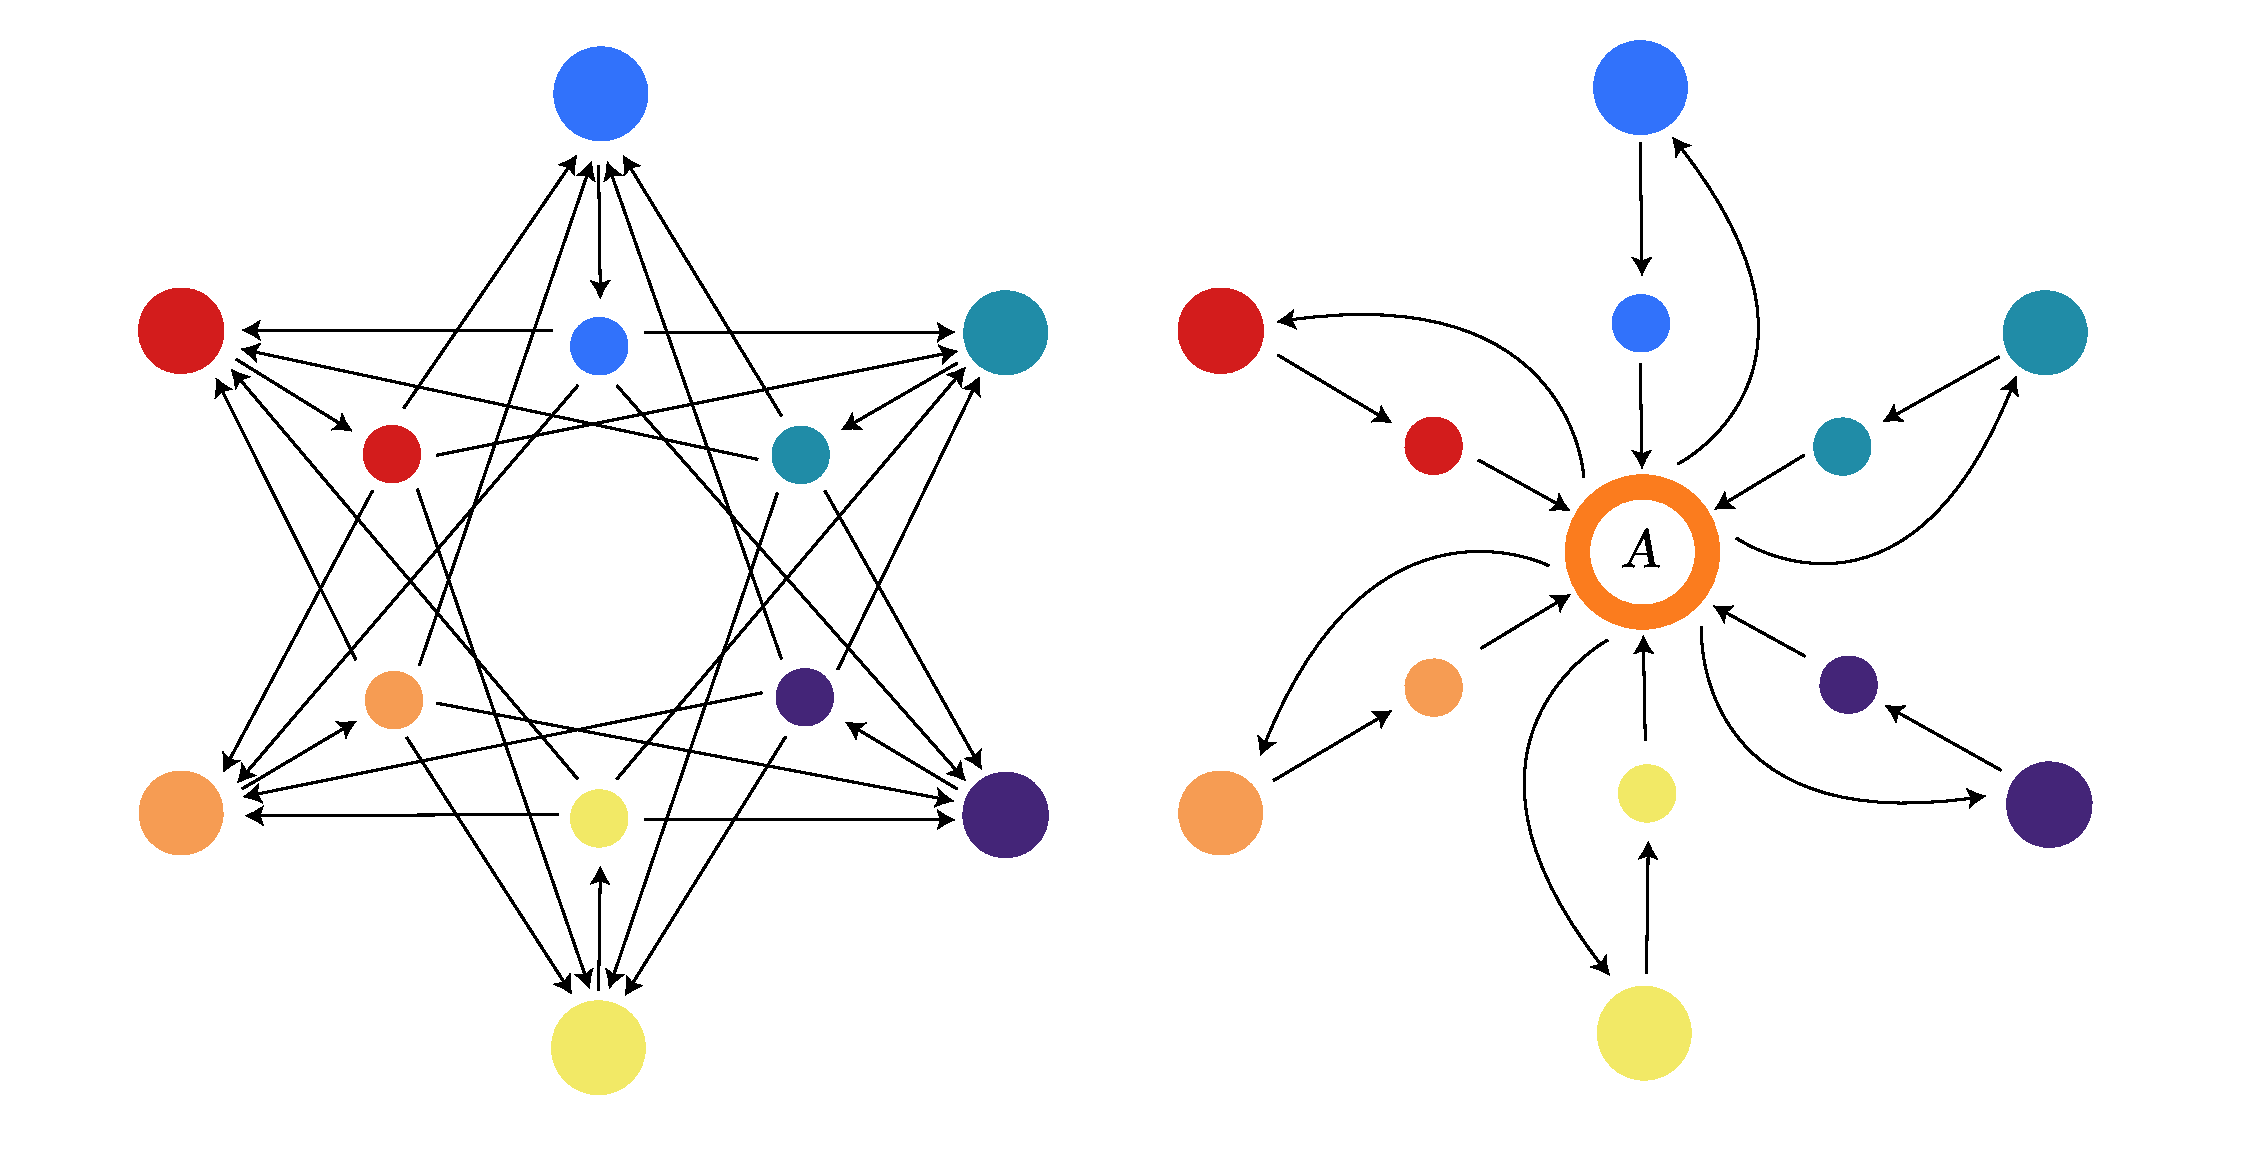
\includegraphics[width=\textwidth]{fig/feed-aggregation-2.pdf}
\caption[Feed aggregation \statusyellow]{Feed aggregation serves to merge information from several source feeds in order to save consumers from duplicate work. \textbf{Left:} 6 nodes involved in group communication (discussing a post, having real time chat, or asynchronous email thread). Each node publishes their contributions as outbox feed updates (small coloured circles). Each participant polls the other's epoch-based feeds, duplicating work with the lookup. \textbf{Right:} the 6 nodes now register  as sources  with an aggregator which polls the nodes' feed and creates indices that aggregate the sources into one data structure which each participant can then pull.}
\label{fig:feed-aggregation}
\end{figure}

A service of this kind can be provided with arbitrary levels of security, yet trustlessly, without relying on reputation. Using consensual data structures for the aggregation, incorrect indexes can be proven using inexpensive and compact inclusion proofs (see \ref{sec:files}) and therefore any challenges related to correctness can be evaluated on chain. Providers face the risk of losing their deposit if a challenge remains unrefuted, which acts as a strong incentive for them to maintain a high quality of service.

\subsection{Integrity \statusyellow}\label{sec:feed-integrity}

We consider a feed to have \emph{integrity} when each of its updates is unambiguous. Formally, this means that for each index, the respective feed identifier is only ever assigned to a single payload. Incidentally, this also implies that the corresponding feed chunk has integrity. As discussed in \ref{sec:single-owner-chunks}, this is a prerequisite for consistent retrieval. 
If the payloads of the successive updates are imagined as blocks of a blockchain, then the criterion of integrity requires feed owners to avoid creating forks in their chain. 

In fact, the integrity of a feed can only be guaranteed by the owner. However, it is important to consider whether the integrity can be effectively checked or enforced. Owners can commit to the integrity of their feeds by staking a deposit on the blockchain, which they stand to lose if they are found to double sign on an update. While this may provide a strong disincentive to fork a feed in the long run, by itself, it does not offer sufficient guarantees to consumers of the feed with respect to integrity. Because of this, we must design indexing schemes that actively enforce this integrity.

\subsubsection{Authoritative version history}

Mutable resource update feeds track versions pretty much the same way as the Ethereum Name Service does.  
When a version is consolidated, for example, of a website, the owner wants to register the content address of the current version. In order to guarantee that there is no dispute over history, the payload needs to incorporate the hash of the previous payload. This imposes the requirement that the payload must be a composite structure. However, if we want the payload to just be a manifest or manifest entry, so that it can be rooted to a URL path or directly displayed, this is not possible. Additionally, if the feed content is not a payload hash, ENS registers a payload hash even though the chunk may not exist on Swarm, thus violating the semantics of ENS.

An indexing scheme which incorporates the previous payload hash into the subsequent index operates in a similar manner to a blockchain. It expresses the owner's unambiguous commitment to a particular history and that any consumer who reads and uses it acknowledges their acceptance of that history. 
Looking up such feeds is only possible by retrieving each update since the last known one. The address refers to the update chunk, so registering the update address both guarantees historic integrity and preserves ENS semantics so that the registered address is just a Swarm reference to a chunk.
Such feeds implement an \gloss{authoritative version history}, i.e. a secure audit trail of the revisions made to a mutable resource. 

\subsubsection{Real-time integrity check}

A deterministically indexed feed provides the ability to perform a \gloss{real-time integrity check}. In the context of feeds that represent blockchains (ledgers/side-chains), integrity refers to having a non-forking and unique chain commitment. The ability to enforce this in real-time allows fast and secure definitions of transaction finality. 

We illustrate this with an example of an off-chain p2p payment network where each node's locked-up funds are allocated to a fixed set of creditors (see more detail in \cite{ethersphere2019swap}). Creditors of the node need to verify the accuracy of the reallocations, i.e. that the total increases are covered by countersigned decreases. 
If a debitor keeps publishing a deposit allocation table for an exhaustive list of creditors, by issuing two alternatives to targeted creditors, the debitors will be able to orchestrate a double spend. Conversely, if there is certainty in the uniqueness of this allocation table, the creditor can confidently conclude finality.

We claim that using Swarm feeds, this uniqueness constraint can be verified in real-time.

The key insight is that meaningfully controlling the responses to a single owner chunk request is impossible: Even if an attacker has control over the entire neighbourhood of the chunk address, there is no systematic way to respond with particular versions to particular requestors.%
%
\footnote{If the chunks are uploaded using the same route, the chunk that comes later will be rejected as already known. If the two chunks originate from different addresses in the network, they might both end up in their local neighbourhood. This scenario will result in inconsistent retrievals depending on which node the request ends up with.}
%
This is due to the inherent ambiguity of the originator of the request in the forwarding Kademlia protocol. Let us imagine that the attacker, with some sophisticated traffic analysis, has the chance of $1/n$ (asymptotic ceiling) to identify the originator and give a differential response. By sending multiple requests from random addresses, however, one can test integrity and consider a consistent response a requirement to conclude finality. The chance that the attacker can give a consistent differential response to a creditor testing with $k$ independent requests is $1/n^k$. With linear bandwidth cost in $k$, we can achieve exponential degrees of certainty about the uniqueness of an update. If a creditor observes consistency in the responses, it can conclude that there is no alternative allocation table.


By requiring the allocation tables to be disseminated as feed updates, we can leverage permissionlessness, availability, and anonymity to enforce feed integrity. If the feed is a blockchain-like ledger, a real-time integrity check translates to fork finality. 


\subsection{Epoch-based 
indexing \statusyellow}\label{sec:epoch-based-feeds}

\yellow{}

In order to use single owner chunks to implement feeds with flexible update frequency, we introduce \gloss{epoch-based feeds}, an indexing scheme where the single owner chunk's identifier incorporates anchors related to the time of publishing. In order to be able to find the latest update, we introduce
an adaptive lookup algorithm. 

\subsubsection{Epoch grid}

An \gloss{epoch} represents a concrete time period starting at a specific point in time, called the \gloss{epoch base time} and has a specific length.  
Period lengths are expressed as powers of 2 in seconds. The shortest period is $2^0 = 1$ second, the longest is $2^{31}$ seconds. 

An \gloss{epoch grid} is the arrangement of epochs where rows (referred to as levels) represent alternative partitioning of time into various disjoint epochs with the same length. Levels are indexed by the logarithm of the epoch length putting level 0 with 1 second epoch length at the bottom by convention, see Figure \ref{fig:epoch-grid}.

\begin{figure}[htbp]
\centering
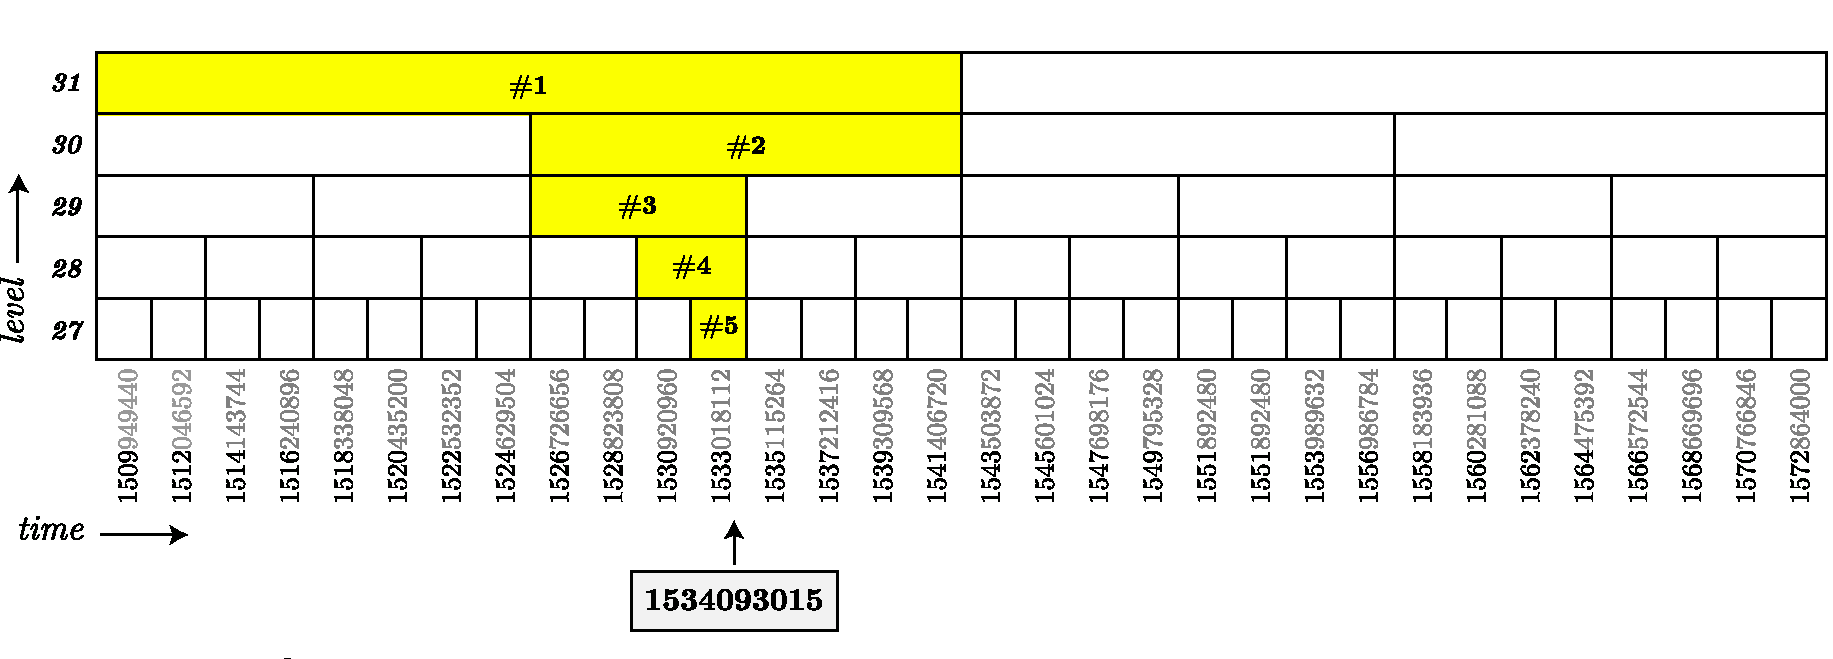
\includegraphics[width=\textwidth]{fig/epoch-grid.pdf}
\caption[Epoch grid with epoch-based feed updates\statusorange]{Epoch grid showing the first few updates of an epoch-based feed. Epochs occupied are marked in yellow and are numbered to reflect the order of updates they represent. }
\label{fig:epoch-grid}
\end{figure}

When representing a epoch-based feed in an epoch grid, each update is assigned to a different epoch in the grid based on their timestamp. In particular, an update is mapped to the longest free epoch that includes the timestamp. This structure gives the series of updates a contiguous structure which allows for easy search. The contiguity requirement implies that by knowing the epoch of the previous update, a subsequent update can be mapped to an epoch unambiguously.


To identify a specific epoch, we need to know both the epoch base time and the level. This pair is called the  \gloss{epoch reference}. To calculate the epoch base time of any given instant in time $t$ at a particular level $l$, we are dropping the $l$ least significant bits of $t$. 
The level requires one byte, and the epoch base time (using linux seconds) 4 bytes so the epoch reference can be serialised in 5 bytes. 
The epoch reference of the very first update of any epoch-based feed is always the same.

\subsubsection{Mapping epochs to feed update chunks}

Feed updates can then be mapped to feed chunks using the serialised epoch reference as the \gloss{feed index}. The topic of the feed hashed together with the index results in the feed identifier used in constructing the single owner chunk that expresses the feed chunk. 

To determine the epoch in which to store a subsequent update, the publisher needs to know where they stored the previous update. If the publisher does not keep track of this, they can use the lookup algorithm to find their last update.



\subsubsection{Lookup algorithm}

When consumers retrieve feeds, they typically will either want to look up the state of the feed at a particular time (historical lookup) or to find the latest update.

If historical lookups based on a \emph{target} time are required, the update can incorporate a data structure mapping timestamps to states. In such cases, finding any update later than the target can be used to deterministically look up the state at an earlier time. 

If no such index is available, historical lookups need to find the shortest filled epoch whose timestamp is earlier than the target. 

To select the best starting epoch from which to walk our grid, we have to assume the worst case scenario, which is that the resource was never again updated after we last saw it. If we don't know when the resource was last updated, we assume 0 as the "last time" it was updated.

We can guess a start level as the position of the first nonzero bit of $\mathit{lastUpdate}\xor \mathit{NOW}$ counting from the left. The bigger the difference among the two times (last update time and now), the higher the level will be.

% In \ref{sec:epoch-based-feeds-appendix}, we walk the reader through an example.

\subsection{Real-time data exchange \statusyellow}\label{sec:feed-as-channel}

Feeds can be used to represent a communication channel, i.e. the outgoing messages of a persona. Such a feed, called an \gloss{outbox feed} can be created to provide email-like communication or instant messaging, or even the two combined. For email-like asynchronicities, \gloss{epoch-based indexing} can be used while for instant messaging, it is best to use deterministic sequence indexing. 
In group chat or group email, confidentiality is handled using an access control trie over the data structure, indexing each party's contribution to the thread. Communication clients can retrieve each group member's feed relating to a thread and merge their timelines for rendering. 

Even forums could be implemented with such an outbox mechanism, however, above a certain number of registered participants, aggregating all outboxes on the client side may become impractical and require index aggregators or other schemes to crowdsource combination of the data.

\subsubsection{Two-way private channels}
 
Private two-party communication can also be implemented using outbox feeds, see Figure \ref{fig:feeds-as-channel}. The parameters of such feeds are set as part of an initial key exchange or registration protocol (see \ref{sec:pss-key-exchange}) which ensures that the parties consent on the indexing scheme as well as the encryption used. 


\begin{figure}[htbp]
  \centering
  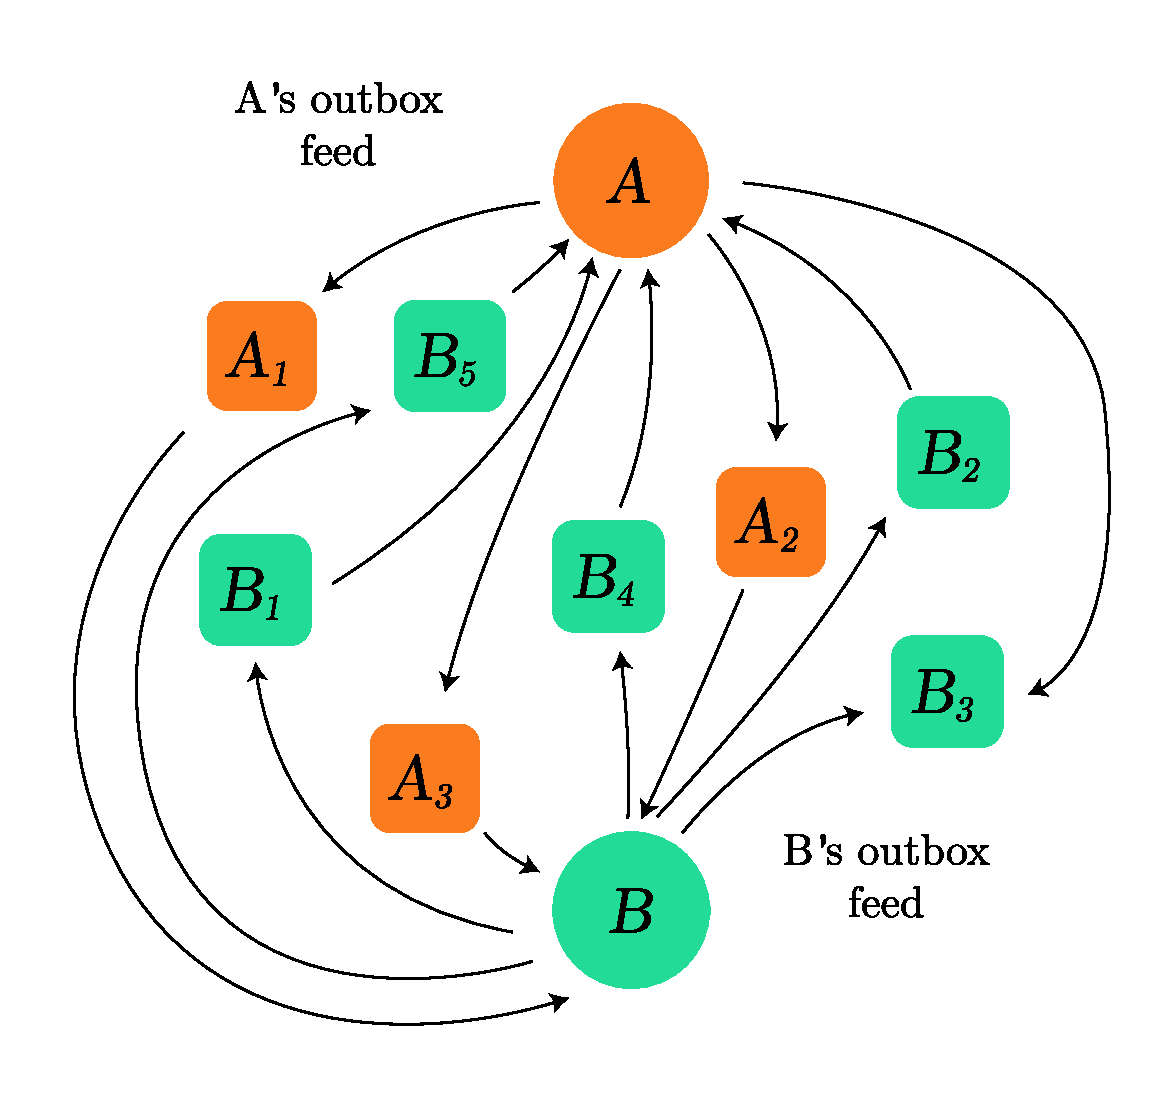
\includegraphics[width=0.7\textwidth]{fig/feeds-as-channel.pdf}  
  \caption[Swarm feeds as outboxes \statusgreen]{Swarm feeds as outboxes for private communication. Outbox feeds represent consecutive messages from a party in a conversation. The indexing scheme can follow a key management system with strong privacy which obfuscates the communication channel itself and renders interception attacks prohibitively expensive.}
\label{fig:feeds-as-channel}
\end{figure}


The real-time series feed used for instant messaging ought to have an indexing scheme with deterministic continuations for at least a few updates ahead. This enables sending retrieve requests for future updates ahead of time, i.e. during or even prior to processing the previous messages. When such retrieve requests arrive at the nodes whose address is closest to the requested update address, the chunk will obviously not be able to be found as the other party will not have sent them yet. However, even these storer nodes are incentivised to keep retrieve requests alive until they expire (see the argument in \ref{sec:retrieval}). This means that up until the end of their time-to-live setting (30 seconds), requests will behave as subscriptions: the arrival of the update chunk triggers the delivery response to the open request as if it was the notification sent to the subscriber. This reduces the expected message latency down to less than twice the average time of one-way forwarding paths, see Figure \ref{fig:outbox-feed-latency}. 


\begin{figure}[htbp]
\includegraphics[width=\textwidth]{fig/outbox-feed-latency.pdf}  
\centering
\caption[Advance requests for future updates \statusgreen]{Advance requests for future updates. The diagram shows the time of a series of events during instant messaging between two parties A and B using outbox feeds. The columns designate the neighbourhood locations of the feed update addresses. Circles show the time of protocol messages arriving: colors indicate the origin of data, empty circles are retrieve requests, full circles are push sync deliveries arriving at the respective neighbourhood. Note that the outbox addresses are deterministic 3 messages ahead so retrieve requests can be sent before the update arrives.

Importantly, latency between one party sending a message $m$ and the other receiving it is shown as $\delta(m)$. Messages $A_3$ and $A_4$ arrive before $A_2$ which can be reported and repaired. If address predictability was only possible for 1 message ahead, both $B_2$ and $B_3$ would have much longer latencies.

Also note that the latency of $B_2$ and $B_3$ are helped by advance requests:  the retrieve requests for $B_4$ and $B_5$ are sent upon receipt of $B_1$ and $B_2$ and arrive at their neighbourhood the same time as the messages $B_2$ and $B_3$ arrive at theirs, respectively. If address predictability was only 1 message ahead, this would also cause both $B_2$ and $B_3$ to have much longer latencies.}
\label{fig:outbox-feed-latency}
\end{figure}


\subsubsection{Post-compromise security}

A key management solution called \gloss{double ratchet} is the de-facto industry standard used for encryption in instant messaging.
It is customary to use the \gloss{extended triple Diffie--Hellmann key exchange} (\gloss{X3DH}) to establish the initial parameters for the double-ratchet key chains (see \ref{sec:pss-key-exchange}).

Double-ratchet combines a ratchet based on a continuous key-agreement protocol with a ratchet based on key-derivation function \cite{perrin2016double}. This scheme can be generalised \cite{alwen2019double} and understood as a combination of well-understood primitives and shown to provide  (1) forward secrecy, (2) backward secrecy,%
%
\footnote{Also known as future secrecy or post-compromise security.}
%
and (3) immediate decryption and message loss resilience.


\begin{figure}[htbp]
\centering
\includegraphics[width=.6\textwidth]{fig/double-ratchet.png}
\caption[Future secrecy for update addresses \statusorange]{Future secrecy for update addresses}
\label{fig:double-ratchet-for-feeds}
\end{figure}

On top of the confidentiality due end-to-end encryption, Swarm offers further resistance to attacks. Due to forwarding Kademlia, the sender is ambiguous and deniable. Due to normal push-sync and pull-sync traffic, messages are also obfuscated. To make it really hard for an attacker, the sequence of indexes can also provide \gloss{future secrecy} if we add more key chains to the double-ratchet machinery. Beside root, sending and receiving encryption key chains, we would need to introduce two more: outgoing and incoming \gloss{outbox index key chains}, see Figure \ref{fig:double-ratchet-for-feeds}. As a result of this measure the underlying communication channel is obfuscated, i.e. intercepting an outbox update chunk and knowing its index, reveals nothing about previous or subsequent outbox update indexes. This makes subsequent messages prohibitively difficult and costly to monitor or intercept.

In \ref{sec:feed-integrity}, we used factoring in the payload hash into the indexing scheme to achieve non-mergeability of chains (unambiguous history). Inspired by this, we propose also to factor in the payload hash into the subsequent feed update index. This results in the additional property called \gloss{recover security},  which, intuitively, ensures that once an adversary manages to forge a message from A to B, then no future message from A to B will be accepted by B.
This is guaranteed if the authenticity of A's  messages to B affects the subsequent \gloss{feed index}. If there is a mismatch (one of the messages was forged), messages will be looked up at the wrong address and therefore the communication channel will be abandoned and a new one is initiated. Such a communication channel represents a completely confidential zero-leak solution for real-time messaging.




\section{Pss: direct push messaging with mailboxing \statusgreen}\label{sec:pss}

\green{}

This section introduces \emph{pss}, Swarm's direct node-to-node push messaging solution. 
Functionalities of and motivation for its existence are playfully captured by alternative resolutions of the term:

\begin{itemize}[noitemsep]
\item \emph{postal service on Swarm} -- Delivering messages if recipient is online or depositing for download if not.
\item \emph{pss is bzz whispered} -- Beyond the association to Chinese whispers, it surely carries the spirit and aspiration of Ethereum Whisper.%
%
\footnote{Whisper is a gossip-based dark messaging system, which is no longer developed. It never saw wide adoption due to its (obvious) lack of scalability. Whisper, alongside Swarm and the Ethereum blockchain, was the communication component of the holy trinity, the basis for Ethereum's original vision of web3.}
%
Pss piggy-backs on Swarm's \gloss{distributed storage} for chunks and hence inherits their full incentivisation for relaying and persistence. At the same time it borrows from Whisper's crypto, envelope structure and API.
\item \emph{pss! instruction to hush/whisper} -- Evokes an effort to not disclose information to 3rd parties, which is found exactly in the tagline for pss: truly zero-leak messaging where beside anonymity and confidentiality, the very act of messaging is also undetectable.
\item  \emph{pub/sub system} -- API allows publishing and subscription to a topic.
\end{itemize}

First, in \ref{sec:trojan}, we introduce Trojan Chunks, i.e. messages to storers that masquerade as chunks whose content address happens to fall in the proximity of their intended recipient. 
\ref{sec:pss-key-exchange} discusses the use of pss to send a contact message to open a real time communication channel.
In \ref{sec:addressed-envelopes}, we explore the mining of feed identifiers to target a neighbourhood with the address of a single owner chunk and present the construct of an addressed envelope. Finally, building on Trojan chunks and addressed envelopes, \ref{sec:notification-requests} introduces update notification requests.

\subsection{Trojan chunks\statusgreen}\label{sec:trojan}

Cutting edge systems promising private messaging often struggle to offer truly zero-leak communication \cite{kwon2016riffle}. While linking the sender and recipient is cryptographically proven to be impossible, resistance to traffic analysis is harder to achieve. Having sufficiently large anonymity sets requires high volumes available at all times. In the absence of mass adoption, guaranteeing high message rate in dedicated messaging networks necessitates constant fake traffic. With Swarm, the opportunity arises to disguise messages as chunk traffic and thereby obfuscate even the act of messaging itself. 

We define a \gloss{Trojan chunk} as a content addressed chunk the content of which has a fixed internal structure, see Figure \ref{fig:trojan-chunk}:

\begin{enumerate}
    \item \emph{span} -- 8 byte little-endian uint64 representation of the length of the message  
    \item \emph{nonce} -- 32 byte arbitrary nonce 
    \item \emph{Trojan message} -- 4064 byte asymmetrically encrypted message ciphertext with underlying plaintext composed of
    \begin{enumerate}
        \item \emph{length} -- 2 byte little-endian encoding of the length of the message in bytes $0\leq l\leq 4030$,
        \item \emph{topic} -- $32$ byte obfuscated topic id   
        \item \emph{payload} -- $m$ bytes of a message 
        \item \emph{padding} -- $4030-m$ random bytes.
    \end{enumerate}
\end{enumerate}

\begin{figure}[htbp]
\centering
\includegraphics[width=\textwidth]{fig/trojan-generic.pdf}
\caption[Trojan chunk or pss message\statusgreen]{A pss message is a Trojan chunk that wraps an obfuscated topic identifier with a Trojan message, which in turn wraps the actual message payload to be interpreted by the application that handles it.}
\label{fig:trojan-generic}
\end{figure}

\begin{figure}[htbp]
\centering
\includegraphics[width=\textwidth]{fig/trojan-chunk-3.pdf}
\caption[Trojan chunk\statusgreen]{The Trojan chunk wraps an asymmetrically encrypted Trojan message.}
\label{fig:trojan-chunk}
\end{figure}

Knowing the public key of the recipient, the sender wraps the message in a trojan message (i.e. prefixing it with length, then padding it to 4030 bytes) then encrypts it using the recipient's public key to obtain the ciphertext payload of the trojan chunk by asymmetric encryption. Then the sender finds a random nonce such that when it is prepended to the payload, the chunk hashes to an address that starts with a \gloss{destination target} prefix. The destination target is a bit sequence that represents a specific neighbourhood in the address space. If the target is a partial address derived as a prefix of the recipient overlay address, matching the target means that the chunk falls in the neighbourhood of the recipient. If only the public key is known, it is assumed that it is the bzz account of the recipient, i.e. their overlay address can be calculated from it%
%
\footnote{Alternative overlays can be associated with a public key, and several public keys can be listened on by a node at a particular address.}
%
(see \ref{sec:overlay-addressing}). The sender then uploads the resulting chunk to Swarm with postage stamps of their choice which then ends up being synced to the recipient address' neighbourhood. If the recipient node is online they receive the chunk for certain provided the bit length of the matching target is greater than the recipient's neighbourhood depth. In practice, targets should be $n+c$ bits long where $n$ is the estimated average depth in swarm and $c$ is a small integer. 

\subsubsection{Receiving Trojan messages}

The recipient only knows that a chunk is a pss message if and when they successfully opened the Trojan message with the private key corresponding to the public key that they advertise as their resident key (see \ref{sec:pss-key-exchange}) and do an integrity check/topic matching. Nodes that want to receive such Trojan Messages will keep trying to open all messages that they are closest to. Forwarding nodes (or anyone else apart from sender and recipient) have no way to distinguish between a random encrypted chunk and a trojan message, which means that communication is perfectly obfuscated as generic chunk traffic.

After the recipient has opened the envelope using asymmetric decryption, there is a combined step of integrity check and topic matching. Knowing the length of the payload (from the first 2 bytes of the message), the recipient takes the payload slice and calculates the Keccak256 hash of it. Now for each topic the client has a subscription to, it then hashes the payload hash together with the topic. If the resulting segment xor-ed with the topic matches the obfuscated topic id in the message then the message is indeed meant as a message with the said topic and the registered handler is called with the payload as argument.

\subsubsection{Mailboxing for asynchronous delivery}

If the recipient is not online the chunk will prevail as any other chunk would, depending on the postage stamp it has. Whenever the recipient node comes online, it pull-syncs the chunks from the neighbourhood closest to it, amongst them all the Trojan chunks, and amongst them their own as yet unreceived messages. In other words, through Trojan messages pss automatically provides asynchronous \emph{mailboxing} functionality, i.e. 
without any further action needed from the sender, even if they are offline at the time that their correspondent has sent them, undelivered messages are preserved and available to the recipient whenever they come online. The duration of mailboxing is controlled with postage stamps in exactly the same way as the storage of chunks, in fact, it is totally indistinguishable.

\subsubsection{Mining for proximity}

The process of finding a hash close to the recipient address is analogous to mining blocks on the blockchain. The nonce segment in a Trojan chunk also plays exactly the same role as a block nonce: it provides sufficient entropy to guarantee a solution. The difficulty of mining corresponds to the length of the destination target: The minimum proximity order required to ensure that the recipient will receive the message needs to be higher than the neighbourhood depth of the recipient%
%
\footnote{It makes sense to use the postage batch uniformity depth (see \ref{sec:postage-stamps}) as a heuristic for the target proximity order when mining a Trojan chunk. This is available as a read-only call to the postage stamp smart contract.}
%
when it comes online, so it is logarithmic in the number of nodes in the network. The expected number of nonces that need to be tried per Trojan message before an appropriate content address is found is exponential in the difficulty, and therefore equal to the number of nodes in the network. As the expected number of computational cycles needed to find the nonce equals the network size, in practice, mining a Trojan will never be prohibitively expensive or slow even for a single node. A small delay in the second range is expected only in a network of a billion nodes and even that is acceptable given that Trojan messages are meant to be used only for one-off instances such as initiations of a channel. All subsequent real-time exchange will happen using the previously described bidirectional outbox model using single owner chunks.


\subsubsection{Anonymous mailbox}

Asynchronous access to pss messages is guaranteed if the postage stamp has not yet expired. The receiver only needs to create a node with an overlay address corresponding to the destination target advertised to be the recipient's resident address.    

One can simply create an anonymous mailbox. An anonymous mailbox can receive pss messages on behalf of a client and then publish those on a separate, private feed so that the intended recipient can read them whenever they come back online.

\subsubsection{Register for aggregate indexing}

As mentioned in \ref{sec:indexing-schemes}, aggregate indexing services help nodes in monitoring sporadic feeds. For instance, a forum indexer aggregates the contribution feeds of registered members. For public forums, off-chain registration is also possible and can be achieved by simply sending a pss message to the aggregator. 


\subsection{Initial contact for key exchange\statusgreen}\label{sec:pss-key-exchange}


Encrypted communication requires a handshake to agree on the initial parameters that are used as inputs to a symmetric key generation scheme. The \gloss{extended triple Diffie--Hellmann key exchange} (\gloss{X3DH}) is one such protocol \cite{marlinspike2016x3dh}, and is used to establish the initial parameters for a post-handshake communication protocol such as the \emph{double-ratchet scheme} discussed earlier in the section on feeds (see \ref{sec:feed-as-channel}). 
In what follows, we describe how the X3DH protocol can be implemented with pss in a serverless setting. 

Swarm's X3DH uses the same primitives as are customary in Ethereum, i.e. secp256k elliptic curve, Keccak256 hash, and a 64-byte encoding for EC public keys. 

The Swarm X3DH protocol is set out to allow two parties to establish a shared secret that forms the input used to determine the encryption keys which will be used during post-handshake two-way messaging. The \emph{initiator} is the party that initiates a two-way communication with the \emph{responder}. The responder is supposed to advertise the information necessary for parties not previously known to the responder to be able to initiate contact. Zero leak communication can be achieved by first performing an X3DH to establish the seed keys used by the double-ratchet protocol for the encryption of data, as well as the feed indexing methodology used. This will enable the responder to retrieve the updates of the outbox feed.

X3DH uses the following keys:%
%
\footnote{The protocol specifies one-time pre-keys for the responder, but these can be safely ignored since they only serve as replay protection, which is solved by other means in this implementation.}

\begin{itemize}[noitemsep]
\item responder long-term public identity key - $K^{\mathrm{ENS}}_r$,
\item responder resident key (aka signed pre-key) - $K^{\mathrm{Res}}_r$,
\item initiator long-term identity key - $K^{\mathrm{ID}}_i$,
\item initiator ephemeral key for the conversation - $K^{\mathrm{EPH}}_i$.
\end{itemize}{}



\begin{figure}[htbp]
   \centering
   \includegraphics[width=\textwidth]{fig/prekey-bundle-feed-update.pdf}
   \caption[X3DH pre-key bundle feed update \statusgreen]{The X3DH pre-key bundle feed update contains the resident key and resident address and is optionally together encrypted with the ENS name hash to prove uniqueness and provide authentication.}
\label{fig:prekey-bundle-feed-update}
\end{figure}


A \gloss{pre-key bundle} consists of all information the initiator needs to know about responder. However, instead of being stored on (usually 3rd-party) servers, this information is instead stored in Swarm. For human-friendly identity management, ENS can be optionally used to provide familiar username based identities. The owner of the ENS resolver represents the long-term public identity key of this persona and is considered authenticated. The long-term identity address can be used to construct an epoch-based feed with a topic id indicating it provides the pre-key bundle for would be correspondents. When communication is initiated with a new identity, the latest update from the feed is retrieved by the initiator, containing the current \emph{resident key} (aka \emph{signed pre-key}) and current \emph{addresses of residence}, i.e. (potentially multiple) overlay destination targets where the persona is expecting she may receive pss messages. The signature in the feed update chunk signs both the resident key (cf. signed pre-key) and the destination targets. The public key that is recovered from this signature gives the long-term identity public key, see Figure \ref{fig:prekey-bundle-feed-update}.


\begin{figure}[htbp]
   \centering
   \includegraphics[width=.8\textwidth]{fig/x3dh-initial-message.pdf}
   \caption[X3DH initial message \statusgreen]{X3DH initial message. Initiator retrieves the ENS owner as well as the latest update of responder's pre-key bundle feed containing the resident key and resident address. Initiator sends their identity key and an ephemeral key to responder's resident address using the resident key for encryption. }
\label{fig:x3dh-initial-message}
\end{figure}


In order to invite a responder to an outbox-feed based private communication channel, the initiator first looks up the responder's public pre-key bundle feed and sends an initial message to the responder (see Figure \ref{fig:x3dh-initial-message}) in which the intent to communicate is indicated. She then shares the parameters required to initiate the encrypted conversation. This consists of the public key of its long-term identity, as well as the public key of the ephemeral key-pair which has been generated just for that conversation. These details are delivered to the potential responder by sending a Trojan pss message addressed to the responder's current address of residence which is also being advertised in their pre-key bundle feed. 

\begin{figure}[htbp]
   \centering
   \includegraphics[width=.6\textwidth]{fig/x3dh.pdf}
   \caption[X3DH secret key \statusgreen]{X3DH secret key. Both parties can calculate the triple Diffie-Hellmann keys and xor them to get the X3DH shared secret key used as the seed for the post-handshake protocol.}
   \label{fig:x3dh}
\end{figure}

After the responder receives this information, both parties have all the ingredients needed to generate the triple Diffie-Hellmann shared secret, see Figure \ref{fig:x3dh}.%
%
\footnote{If the X3DH does not use one-time pre-keys, the initial message can in theory be re-sent by a third party and lead the responder to assume genuine repeated requests. Protocol replay attacks like this are eliminated if the post-handshake protocol adds random key material coming from the responder. 
But the initial Trojan message can also be required to contain a unique identifier, e.g. the nonce used for mining the chunk. Reusing the id is not possible since it leads to the same chunk.}
%
This shared secret constitutes the seed key for the double-ratchet continuous key agreement protocol as used in the signal protocol. The double-ratchet scheme provides forward secrecy and post-compromise security to the end-to-end encryption. By applying separate key-chains for the outbox feed's indexing scheme, additional \gloss{recover security}, i.e. resilience to message insertion attack, can be achieved. Most importantly, however, by adding forward and backward secrecy to outbox addresses, the communication channel is obfuscated, which renders sequential message interception contingent on the same security assumptions as encryption and therefore eliminates the only known attack surface for double-ratchet encryption. The obfuscation and deniability of the channel based on outbox feeds, together with the initial X3DH message being disguised indistingushable as a chunk warrants designating this as  zero-leak communication.

\subsection{Addressed envelopes\statusgreen}\label{sec:addressed-envelopes}

\subsubsection{Mining single owner chunk addresses}

The question immediately arises whether it makes sense to somehow mine single owner chunks. Since the address in this case is the hash of a 32 byte identifier and a 20 byte account address, the id provides sufficient entropy to mine addresses even if the owner account is fixed. So for a particular account, if we find an id such that the resulting single owner chunk address is close to a target overlay address, the chunk can be used as a message in a similar way to Trojan chunks. Importantly, however, since the address can be mined before the chunk content is associated with it, this construct can serve as an \gloss{addressed envelope}.

Let us make explicit the roles relevant to this construct:

\begin{itemize}[noitemsep]
\item \emph{issuer} ($I$) - creates the envelope by mining an address. 
\item \emph{poster} ($P$) - puts the content into the envelope and posts it as a valid single owner chunk to Swarm.
\item \emph{owner} ($O$) - possesses the private key to the account part of the address and can thus sign off on the association of the payload to the identifier. This effectively decides on the contents of the envelope.
\item \emph{target} ($T$) - the constraint for mining: a bit sequence that must form the prefix of the mined address. It represents a neighbourhood in the overlay address space where the envelope will be sent. The length of the target sequence corresponds to the difficulty for mining. The longer this target is, the smaller the neighbourhood that the envelope will be able to reach.
\item \emph{recipient} ($R$) - the party whose overlay address has the target sequence as its prefix and therefore the destination of the message
\end{itemize}

The envelope can be perceived as open: since the poster is also the owner of the response single owner chunk, they are able to control what content is put into the chunk. By constructing such an envelope, the issuer effectively allows the poster to send an arbitrary message to the target without the computation requirement needed to mine the chunk. See Figure \ref{fig:addressed-envelope-events}. 


\begin{figure}[htbp]
   \centering
   \includegraphics[width=0.75\textwidth]{fig/prepaid-addressed-envelopes-events.pdf}
   \caption[Stamped addressed envelopes timeline of events \statusgreen]{Stamped addressed envelopes timeline of events. Issuer $I$ creates the envelope encrypted for $P$ with an identifier such that $P$ as the single owner of the chunk, produces an address that falls in the recipient $R$'s neighbourhood. As a result (only) $P$ can fill the envelope with arbitrary content and then use simple push-syncing to post it to $R$.}
   \label{fig:addressed-envelope-events}
\end{figure}

All the poster needs to do when they wish to send a message to the recipient is to create a Trojan message and sign it against the identifier using the private key of the same account the issuer used as an input when they mined the address. If they do this, the chunk will be valid. See Figure \ref{fig:addressed-envelope}.


\begin{figure}[htbp]
   \centering
   \includegraphics[width=\textwidth]{fig/addressed-envelope.pdf}
   \caption[Stamped addressed envelopes \statusgreen]{A stamped addressed envelope issued for $P$ and addressed to $R$ consists of an identifier which is mined so that when used to create a single owner chunk owned by $P$, it produces an address which falls within $R$'s neighbourhood. This allows $P$ to construct a message, sign it against the identifier and using the postage stamp, post it using the network's normal push-syncing to $R$ for free. }
   \label{fig:addressed-envelope}
\end{figure}

\subsubsection{Pre-paid postage}

These chunks behave in the same way as normal Trojan messages, with their privacy properties being the same if not somewhat better since the issuer/recipient can associate a random public key with which the message is encrypted, or even use symmetric encryption. If a postage stamp is pre-paid for an address and given to someone to post later, they can use push-sync to send the chunk to the target without the poster needing to pay anything, the cost of this having already been covered by the \gloss{stamped addressed envelope}. Such a construct effectively implements \emph{addressed envelopes with pre-paid postage} and serves as a base layer solution for various high-level communication needs: 1) push notifications about an update to subscribers without any computational or financial postage burden on the sender 2) free contact vouchers 3) zero-delay direct message response.  


\subsubsection{Issuing a stamped addressed envelope}

Issuing a stamped addressed envelope involves the following process:

\begin{enumerate}[noitemsep]
\item \emph{assume} issuer $I$, prospective poster $P$, and prospective recipient $R$ with public keys $K_I, K_P, K_R$ and overlay addresses $A_I, A_P, A_R$.
\item \emph{mine} -- $I$ finds a nonce $N_R$ such that when used as an identifier to create a \gloss{single owner chunk}, the  address of the chunk hashes to $H_R$ which is in the nearest neighbourhood of $A_R$.
\item \emph{pay postage} -- $I$ signs $H_R$ to produce a witness for an appropriate postage payment to produce stamp $PS_R$.
\item \emph{encapsulate} -- package $N_R$ and $PS_R$ which represent the pre-paid envelope pre-addressed to recipient address and encrypt it with $K_P$ then wrap it as a Trojan chunk.
\item \emph{mine} -- find a nonce $N_P$ such that the Trojan chunk hashes to $H_P$ which is in the nearest neighbourhood of $A_P$. 
\end{enumerate}




\subsubsection{Receiving a stamped addressed envelope}

A prospective poster $P$ is assumed to receive a a Trojan message consisting of pre-paid envelope $E$. In order to open it, she carries out the following steps:

\begin{enumerate}[noitemsep]
    \item \emph{decrypt} message with the private key belonging to $K_P$
    \item \emph{deserialise} unpack and identify $PS_R$ and $N_R$, extract $H_R$ from $PS_R$
    \item \emph{verify} postage stamp $PS_R$ and check if $N_R$ hashed with the account for $K_P$ results in $H_R$ to ensure the associated address is in fact owned by $P$.
    \item \emph{store} $N_R$ and $PS_R$ 
\end{enumerate}

\subsubsection{Posting a stamped addressed envelope}

When the poster wants to use the envelope to send an arbitrary message $M$ to $R$ (with recipient $R$ potentially unknown to the sender), they must follow the following steps:

\begin{enumerate}[noitemsep]
\item \emph{encrypt} the message content $M$ with $K_R$ to create a payload and wrap it in Trojan message $T$
\item \emph{hash} the encrypted Trojan message resulting in $H_T$
\item \emph{sign} $H_T$ against the identifier $N_R$ using the private key belonging to $K_P$ producing signature $W$
\item \emph{encapsulate} nonce $N_R$ as id, the signature $W$ and the Trojan message $T$ as the payload of a valid single owner chunk with address $H_R$
\item \emph{post} the chunk with the valid stamp $PS_R$
\end{enumerate}

\subsubsection{Receiving a posted addressed envelope}

When $R$ receives chunk with address $H_R$

\begin{enumerate}[noitemsep]
\item \emph{verify} postage stamp $PS_R$ and validate the chunk as a single owner chunk with payload $T$.
\item \emph{decrypt} $T$ with the private key belonging to $K_R$.
\item \emph{deserialise} the plaintext as a Trojan message, identify the message payload $M$ and check its integrity.
\item \emph{consume} $M$.
\end{enumerate}

\subsection{Notification requests\statusgreen}\label{sec:notification-requests} 

\yellow{new}

This section elaborates on the concept of addressed envelopes and presents three flavours, each implementing different types of notifications.

\subsubsection{Direct notification from publisher}

If an issuer wants a recipient to be notified of the next activity on a feed, she must construct a stamped addressed envelope embedded in a regular Trojan message and send it to the publisher, see Figure \ref{fig:direct-notification}. If the issuer is also the recipient, then the account that is used in the request and the one in the response envelope may be one and the same. 


When the feed owner publishes an update to her feed, the reference to the update chunk is put into the envelope and is sent to the recipient. More formally, the publisher creates a single owner chunk from the identifier representing the pre-addressed envelope and therefore, as the owner, signs off on the identifier associated with the feed update content as the payload of the single owner chunk. Right after this, the same publisher acting as the poster, push-syncs the chunk to the swarm. This construct is called \gloss{direct notification from publisher}. 

\begin{figure}[htbp]
   \centering
   \includegraphics[width=\textwidth]{fig/direct-notification.pdf}
   \caption[Direct notification request and response \statusgreen]{A direct notification request contains a reference to a feed and wraps a pre-paid envelope mined for $P$ (the publisher or a known distributor of the feed) and addressed to recipient $R$. The response is identical to the process used for generic stamped addressed envelopes and only differs in that the message is supposed to be the feed update or a reference to its content.}
   \label{fig:direct-notification}
\end{figure}

The Trojan message specifies in its topic that it is a notification and is encrypted using the public key. As the address is mined to match the recipient overlay address on a sufficiently long prefix, the message ends up push-synced to the recipient's neighbourhood. Whenever the recipient comes online and receives the chunk by push-sync it detects that it is intended as a message. It can be identified as such either by decrypting the chunk content successfully with the key for the address they had advertised, or in case that the recipient has issued the pre-addressed envelope themselves, simply by looking it up the against the record of the address they saved when it was issued.  See Figure \ref{fig:direct-notification-events} for the timeline of events.


\begin{figure}[htbp]
   \centering
    \includegraphics[width=0.8\textwidth]{fig/direct-notification-events.pdf}
   \caption[Direct notification from publisher timeline of events \statusgreen]{Direct notification from publisher timeline of events. Issuer $I$ constructs a prepaid envelope for the publisher or a known distributor of the feed $P/F$ and addressed to recipient $R$. Together with a feed topic $I$, it is sent to $P/F$ wrapped in a pss trojan message. $P/F$ receives it and stores the request. When they publish the update, they wrap it in the envelope, i.e. sign the identifier received from $I$ against the feed update notification message and post it as a chunk, which $R$ will receive and hence, be notified of the feed update. }
   \label{fig:direct-notification-events}
\end{figure}


Notifications coming from publishers directly enable the poster to put arbitrary content into the envelope. The poster is at the same time the owner so that they can sign off on any content against the identifier when posting the envelope. In order for the issuer to be able to create the notification chunk address in advance, the prospective poster's account must be known. However, the feed update address need not be fixed, so this scheme remains applicable to (sporadic) epoch-based feeds.

\subsubsection{Notification from neighbourhood}

Assume there is a feed whose owner has not revealed their overlay (destination target) or refuses to handle notifications.  The feed is updated sporadically using simple sequential indexing and therefore polling is not feasible when it comes to looking up the latest update, especially as the consumer can go offline any time.
Is there a way for consumers to still get notified? 

We introduce another construct, a \gloss{neighbourhood notification} which works without the issuer of the notification knowing the identity of prospective posters. It presupposes, however, that the content or at least the hash of the content is known in advance so that it can be signed by the issuer themselves.


An issuer wants a recipient to be notified of the next update. The issuer can create a \gloss{neighbourhood notification} request, simply a Trojan chunk wrapping a message. This message contains an addressed envelope (identifier, signature and postage stamp) that the poster can use to construct the single owner chunk serving as the notification. Note that the notification message need not contain any new information, merely the fact of receiving it is sufficiently informative to the recipient. In order to indicate what it is a notification of, the notifications payload contains the feed update address. Upon receiving the notification, the receiver can then simply send a regular retrieve request to fetch the actual feed update chunk containing or pointing to the content of the message. See Figure \ref{fig:notification-from-neighbourhood} for the structure of neighbourhood notifications and notification requests.
                                

\begin{figure}[htbp]
\centering
\includegraphics[width=\textwidth]{fig/notification-from-neighbourhood.pdf}
\caption[Neighbourhood notifications \statusgreen]{Neighbourhood notification requests are not only including identifier and postage stamp but also a notification message together with the signature attesting it against the address. Thus $P$ needs to construct the actual notification and when publisher $F$ posts their update to $P$-s neighbour, $P$ can post the notification to recipient $R$.}
\label{fig:notification-from-neighbourhood}
\end{figure}

If the notification needs only to contain the feed update address as its payload then associating it with the identifier can be signed off by the issuers themselves. This signature together with the identifier should be considered a necessary component of the envelope and must be sent as part of the notification request.
Unlike the \emph{open} envelopes used with publishers directly, neighbourhood notifications can be viewed as \emph{closed} envelopes, where the content is sanctioned by the issuer in advance. 

Now the issuer and not the poster becomes the owner of the chunk and the signature is already available to the poster when they create and post the notification. As a consequence no public key or account address information is needed from the poster. In fact, the identity of the poster does not need to be fixed, any peer could qualify as a candidate poster. Issuers therefore can send the notification request to the neighbourhood of the feed update chunk. The nearest neighbours will keep holding the request chunk as dictated by the attached postage stamps until they receive the appropriate feed update chunk that indicates the receipt of the notification. See Figure \ref{fig:neighbourhood-notification-events} for the timeline of events when using neighbourhood notifications.

\begin{figure}[htbp]
\centering
\includegraphics[width=0.8\textwidth]{fig/neighbourhood-notification-events.pdf}
\caption[Neighbourhood notification timeline of events \statusgreen]{Neighbourhood notification timeline of events. Issuer $I$ mines an identifier for a single owner chunk with themselves as owner such that the chunk address falls in recipient $R$'s neighbourhood. The issuer, being the owner also must sign the identifier against a prefabricated reminder and remember which node should be notified. When $P$ syncs the feed update the notification is sent to $R$, delivered by the usual push-syncing.}
\label{fig:neighbourhood-notification-events}
\end{figure}
  

But how can we make sure that notifications are not sent too early or too late? While the integrity of notification chunks is guaranteed by the issuer as their single owner, measures must also be taken to prevent nodes that manage the notifications from sending them before the update should actually arrive. It would be ideal if the notification could not be posted before the arrival of the update, otherwise false alarms could be generated by malicious nodes that service the request.

A simple measure is to encrypt the message in the request  message symmetrically with a key that is only revealed to the prospective poster when they receive the feed update, for instance, the hash of the feed update identifier.
In order to reveal that the notification request needs to be matched on arrival of the feed update, the topic must be left unencrypted, so here we do not encrypt the pss envelope asymmetrically but only the message and symmetrically.

Note that the feed update address as well as identifier can be known if the feed is public, so neighbourhood notifications are to be used with feeds whose subsequent identifiers are not publicly known.

\subsubsection{Targeted chunk delivery}

Normally, in Swarm's DISC model, chunks are requested with retrieve requests, which are forwarded towards the neighbourhood designated by the requested chunk address (see \ref{sec:retrieval}). The first node on the route that has the chunk will respond with it and the chunk is delivered as a backwarded response travelling back along the same route that the request has taken. In certain cases, however, it may be useful to have a mechanism to request a chunk from an arbitrary neighbourhood where it is known to be stored and send it to an arbitrary neighbourhood where it is known to be needed. A construct called \gloss{targeted chunk delivery} is meant for such a use case: the request is a Trojan pss message while the response, the delivery, must be a single owner chunk wrapping the requested chunk, with an address mined to fall into the neighbourhood of the recipient.  


\begin{figure}[htbp]
\centering
\includegraphics[width=\textwidth]{fig/targeted-chunk-delivery.pdf}      
\caption[Targeted chunk deliveries \statusgreen]{Targeted chunk deliveries are similar to neighbourhood notifications in that they are not only pre-addressed and pre-paid but also pre-signed. Similarly, the identifier is mined so that given issuer $I$ as the owner, it produces an chunk address that falls in recipient $R$'s neighbourhood. Here the issuer signs the identifier against the hash of a content addressed chunk that they want to see posted to $R$. If the targeted chunk delivery request lands with any node that has the chunk in question, they can use the envelope and the content of the chunk to produce a valid response which is a single owner chunk wrapping a content addressed chunk.}
\label{fig:targeted-chunk-delivery}
\end{figure}

\begin{figure}[htbp]
\centering
\includegraphics[width=.8\textwidth]{fig/targeted-chunk-delivery-events.pdf}
\caption[Targeted chunk delivery timeline of events\statusgreen]{Targeted chunk delivery timeline of events. Uploader $U$ uploads a chunk to Swarm and it lands with a storer node $S$. Nodes within $P$ replicate (and pin) this chunk. Now, if issuer $I$ wants this chunk delivered to $R$, it will take the prepaid envelope addressed to $R$ and sends it to the neighbourhood of a known host unencrypted so that anyone who has the chunk can construct the notification and send or store it for later.}
\label{fig:targeted-chunk-delivery-events}
\end{figure}



These 'chunk-in-a-soc' responses are structurally similarly to neighbourhood notifications in that the payload's hash is already known (the content address of the chunk requested). The requestor can then sign off on its association with the identifier which, along with the signature, is sent as part of the request, see Figure \ref{fig:targeted-chunk-delivery-events}. A node that got the request only needs to have the requested chunk stored and they can construct the response as a valid single owner chunk addressed to the recipient's neighbourhood.
This makes the request generic, i.e. not fixed to the identity of the prospective poster. Therefore it can be sent to any neighbourhood that requires the content. Even multiple requests can be sent simultaneously: due to the uniqueness of the valid response, multiple responses cannot hurt chunk integrity (see \ref{sec:single-owner-chunks} and \ref{sec:feed-integrity}). Targeted delivery is used in missing chunk recovery, see \ref{sec:recovery-chunks}.

The difference is that neighbourhood notifications are not giving any new information while targeted chunk delivery supplies the chunk data. Also, a chunk delivery wrapped in a single owner chunk uses no message wrapping and has no topic. Neither request nor response uses encryption.
A consequence of not using encryption is that, if there are multiple tartgets, it is sufficient that the initial Trojan request matches any one of these targets. 

Table \ref{tab:notifications} summarises various properties of the three notification-like constructs.

\begin{table}[htpb]
    \centering
    \begin{tabular}{c|c|c|c|c|}
    type & owner & poster & request encryption & notification  \\\hline
         direct & poster & publisher & asymmetric on pss & feed update  content\\
         neighbourhood & issuer & any & symmetric on envelope & feed update arrival\\
         targeted delivery & issuer & any & none & chunk content\\
    \end{tabular}
    \caption[Feed update notifications]{Requests of and responses to types of feed update notifications and targeted chunk delivery.}
    \label{tab:notifications}
\end{table}

\chapter{Persistence \statusgreen}\label{sec:persistence}


In this chapter, we focus on data persistence, i.e. the ways of making sure that content stays available on Swarm. 
We introduce error coding schemes, which can provide cross-neighbourhood redundancy to secure availability against churn at a cost of the storage overhead. 
In particular \glossplural{erasure code} (\ref{sec:erasure}) and \glossplural{entanglement code}  %(\ref{sec:entanglements}) 
provide redundancy optimised for documents with different access patterns.
% First we discuss how popular content stays alive due to opportunistic caching (\ref{sec:caching}).  
After introducing the notion of local pinning in \ref{sec:reupload}, i.e. the ability to mark content as sticky in your Swarm local storage, we will present ways in which this can help achieve global persistence across the network through \emph{stewardship}. We define a \gloss{missing chunk notification protocol}, which allows content maintainers to make sure their published content is restored in the event of some chunks being garbage collected, by proxying retrieval through select \glossplural{pinner} of the content.

In Section \ref{sec:dream}, we discuss how an immutable chunk store can support user-controlled deletion of content.
% Finally, in \ref{sec:insurance}, we present the holy grail, that is, decentralised file insurance: combining the concepts of the postage lottery and missing chunk notifications, Swarm offers a protocol that enables users to pay other nodes to keep their content available. While ordinary storer nodes are rewarded for storing chunks via the postage lottery, for a higher premium, staked nodes will promise to take responsibility for storing and responding to requests for chunks, accepting the risk of punitive measures that will be imposed on them in the event that the insured data does not remain available to the network.


% \section{Redundancy, latency and repair \statusgreen}\label{sec:repair}



\section{Cross-neighbourhood redundancy: erasure codes and dispersed replicas \statusgreen}\label{sec:erasure}
\green{}

First, in \ref{sec:error-correcting-codes}, we introduce \glossplural{erasure code} and their application to files in Swarm in \ref{sec:erasure-bmt}. In \ref{sec:dispersed-replicas}, we present a construct that enables cross-neighbourhood redundancy for singleton chunks that completes erasure coding. Finally, in \ref{sec:strategies}, we explore systematic codes that facilitate various retrieval strategies of erasure-coded files, while preserving random access capabilities.

\subsection{Error correcting codes \statusgreen}\label{sec:error-correcting-codes}
% \enlargethispage*{\baselineskip}
%

\emph{Error correcting codes} are widely utilised in the context of data storage and transfer to ensure data integrity even in the face of a system fault. Error correction schemes define how to rearrange the original data by adding redundancy to its representation before upload or transmission (\emph{encoding}\,) so that it can correct corrupted data or recover missing content upon retrieval or reception (\emph{decoding}\,). The different schemes are evaluated by quantifying their strength (\emph{tolerance}, in terms of the rate of data corruption and loss) as a function of their cost (\emph{overhead}, in terms of storage and computation). 

In the context of  computer hardware architecture, synchronising arrays of disks is crucial to provide resilient storage in data centres.
In \emph{erasure coding}, %
%
%\footnote{\cite{buterin2014erasure}}
%
in particular, the problem can be framed as follows: How does one encode the stored data into shards distributed across the disks so that the data remains fully recoverable in the face of an arbitrary probability that any one disk becomes faulty?
Similarly, in the context of Swarm's distributed immutable chunk store, the problem can be reformulated as follows: How does one encode the stored data into chunks distributed across neighbourhoods in the network so that the data remains fully recoverable in the face of an arbitrary probability that any one chunk is not retrievable?%
%
\footnote{%
It is safe to assume that the retrieval of any one chunk will fail with equal and independent probability.}

\gloss{Reed-Solomon coding} (\gloss{RS}) \cite{lubyetal1995CRS,plank2006optimizing,li2013erasure} 
is the father of all  error correcting codes and also the most widely used and implemented.%
%
\footnote{%
For a thorough comparison of an earlier generation of implementations of RS, see \cite{plank2009performance}.}
% 
When applied to data of $m$ fixed-size blocks (message of length $m$), it produces an encoding of $m+k$ \emph{codewords} (blocks of the same size) 
in such a way that having any $m$ out of $m+k$ blocks is enough to reconstruct the original data. Conversely, $k$ puts an upper bound on the number of \emph{erasures} allowed (number of blocks unavailable) for full recoverability, i.e., it expresses (the maximum) \emph{loss tolerance}.%
%
\footnote{Error correcting codes that has a focus on correcting data loss are referred to as \emph{erasure codes}, a typical scheme of choice for distributed storage systems \cite{balaji2018erasure}.}
%
$k$ is also the count of \emph{parities}, quantifying the data blocks added during the encoding on top of the original volume, i.e., it expresses \emph{storage overhead}. While RS is, therefore, optimal for storage (since loss tolerance cannot exceed the storage overhead), 
it has high bandwidth demands%
%
\footnote{Both the encoding and the decoding of RS codes takes $O(mk)$ time (with $m$ data chunks and $k$ parities). However, we found computational overhead both insignificant for a network setting as well as undifferentiating.}
%
for local repair processes.%
%
\footnote{Entanglement codes \cite{estrada2018alpha, estrada2019building} require a minimal bandwidth overhead for a local repair, but at the cost of storage overhead that is in multiples of $100\%$.}
%
The decoder needs to retrieve $m$ chunks to recover a particular unavailable chunk. 
Hence, ideally, RS is used on files which are supposed to be downloaded in full,%
%
\footnote{Or in  fragments large enough  to include the data span over which the encoding is defined, such as videos.}
%
 but it is inappropriate for use cases needing only local repairs.%
%
\footnote{Use cases requiring random access to small amounts of data (e.g., path lookup) benefit from simple replication to optimise on bandwidth, which is suboptimal in terms of storage \cite{weatherspoon2002erasure}.}

When using RS, it is customary to use \emph{systematic} encoding, which means that the original data forms part of the encoding, i.e., the parities are actually added to it.%
%
%
%\footnote{Our library of choice implementing exactly such a scheme is \url{https://github.com/klauspost/reedsolomon}.}
% 
%


\subsection{Erasure coding in the Swarm hash tree \statusgreen}
\label{sec:erasure-bmt}

Swarm uses the \emph{Swarm hash tree} to represent files. This structure is a Merkle tree \cite{merkle1980protocols}, whose leaves are the consecutive segments of the input data stream. These segments are turned into chunks and are distributed among the Swarm nodes for storage. The consecutive chunk references (either in the form of an address or an address and an encryption key) are written into a chunk on a higher level.
These so-called \emph{packed address chunks} (PACs) constitute the intermediate chunks of the tree.
The branching factor $b$ is chosen so that the references to its children fill up a full chunk.
With a reference size of 32 or 64 (hash size 32) and a chunk size of 4096 bytes, $b$ is 128 for unencrypted, and 64 for encrypted content 
(see Figure \ref{fig:Swarm-hash-split}).


\begin{figure}[!ht]
   \centering
   \input{fig/Swarm-hash-split.tex}
   \caption[Swarm hash split \statusgreen]{The Swarm tree is the data structure encoding how a document is split into chunks.}
   \label{fig:Swarm-hash-split}
\end{figure}

Note that on the right edge of the hash tree, the last chunk of each level may be shorter than 4K: in fact, unless the file is exactly $4\cdot b^n$ kilobytes long, there is always at least one \emph{incomplete chunk}.  Importantly, it makes no sense to wrap a single chunk reference in a PAC, so it is attached to the first level where there is open chunks. Such \emph{"dangling" chunks} will appear if and only if the file has a zero digit in its $b$-ary representation. 

During file retrieval, a Swarm client starts from the root hash reference and retrieves the corresponding chunk. Interpreting the metadata as encoding the span of data subsumed under the chunk, it decides that the chunk is a PAC if the span exceeds the maximum chunk size. 
In case of standard file download, all the references packed within the PAC are followed, i.e., the referenced chunk data is retrieved. 

PACs offer a natural and elegant way to achieve consistent redundancy within the swarm hash tree.
The input data for an instance of erasure coding is the chunk data of the children, with the equal-sized bins corresponding to the chunk data of the consecutive references packed into it. The idea is that instead of having each of the $b$ references packed represent children, only $m$ would, and the rest of the $k=b-m$ would encode RS parities (see Figure \ref{fig:Swarm-hash-erasure}).


The \emph{chunker} algorithm that incorporates PAC-scoped RS encoding would work as follows: 

\begin{enumerate}[noitemsep]
\item Set the input to the actual data level and produce a sequence of chunks from the consecutive 4K segments of the data stream. Choose $m$ and $k$ such that $m+k=b$ is the branching factor (128 for unencrypted, and 64 for encrypted content).
\item Read the input one chunk at a time. Count the chunks by incrementing a counter $i$. 
\item Repeat Step 2 until either $i = m$ or there's no more data left.
\item Use the RS scheme on the last $i\leq m$ chunks to produce $k$ parity chunks resulting in a total of $n = i+k \leq b$ chunks.
\item Concatenate the references of all these chunks to result in a packed address chunk (of size $h\cdot n$ of the next level) of the level above. If this is the first chunk on that level,  set the input to this level and spawn this same procedure from Step 2. 
\item When the input is consumed, signal the end of input to the next level and quit the routine. If there is no next level, record the single chunks as the root chunk and use the reference to refer to the entire file.
\end{enumerate}



\begin{figure}[htbp]
   \centering
   \resizebox{1\textwidth}{!}{
        \input{fig/Swarm-hash-erasure.tex}
   }
   \caption[Swarm hash erasure \statusgreen]{The Swarm tree with extra parity chunks using $m=112$ out of $n=128$ RS encoding. Chunks $P_{0}$ through $P_{15}$ are parity data for chunks $H_0 $ through $H_{111}$ on every level of intermediate chunks.}
   \label{fig:Swarm-hash-erasure}
\end{figure}


This pattern repeats itself all the way down the tree. Thus, hashes $H_{m+1}$ through $H_{127}$ point to parity data for chunks pointed to by $H_0$ through $H_{m}$. Since parity chunks $P_i$ do not have children, the tree structure does not have uniform depth.

\subsection{Incomplete chunks and dispersed replicas}
\label{sec:dispersed-replicas}

If the number of file chunks is not a multiple of $m$, it is not possible to proceed with the last batch in the same way as the others. We propose that we encode the remaining chunks with an erasure code that guarantees at least the same level of security as the others.% 
%
\footnote{Note that this is not as simple as choosing the same redundancy. For example, a $50\text{-out-of-}100$ encoding is much more secure against loss than a $1\text{-out-of-}2$ encoding, even though the redundancy is $100\%$ in both cases.} 
%
Overcompensating, we still require the same number of parity chunks even when there are fewer than $m$ data chunks.

This leaves us with only one corner case: it is not possible to use our $m\text{-out-of-}n$ scheme on a single chunk ($m=1$) because it would amount to $k+1$ copies of the same chunk. The problem is that copies of the same chunk all have the same hash and therefore are automatically deduplicated. Whenever a single chunk is left over ($m=1$) (which is always the case for the root chunk itself), we would need to replicate the chunk in a way that (1) ideally, the replicas are dispersed in the address space in a balanced way, yet (2) their address can be known by retrievers who ideally only know the reference to the original chunk's address.%
%
\footnote{We could create replicas by having the chunk data as the payload of one of more single owner chunks with an address that is deterministically derivable using the content owner's public key and the original root hash. This method has the disadvantage that replicas produced this way are not reuploadable by parties other than the publisher.}

The solution is to reference the root hash with its BMT root hash (before it is hashed with the metadata). By making the metadata fully or partially non-semantic, we gain the flexibility to generate entropy to mine the overall chunk hash into a sufficient number of neighbourhoods. This construct is called \glossplural{dispersed replica} and the detailed method for finding them is as follows:

Let's assume $h$ is the BMT root hash of the chunk.
Given $n$ bits available to find a nonces to generate  $2^k$  perfectly balanced replicas, initialise a chunk array $\rho$ of length $2^k$ and start with $i=0$ and $C=0$.

\begin{enumerate}[noitemsep]
    \item create the metadata by copying the bits of the big-endian binary encoding of $i$ onto the $n$ available bits, resulting in the metadata bytes $m$.
    \item calculate the the chunk hash by prepending      $m$ to $h$ and use the Keccak256 base hash to hash them $a_i:=H(m\concat h)$, and record $c_i=\mathit{CAC}(d,m)$
    \item calculate the bin this hash belongs to by decoding $k$-bit prefix as big-endian binary number $j$ between $0\leq j<2^k$.
    \item if $\rho\idx{j}$ is unassigned, then let $\rho\idx{j}:=c_i$ and increment $C$.
    \item if $C=2^k$, then quit
    \item increment $i$, if $i=2^n$, then quit
    \item repeat from Step 1 
\end{enumerate}

With this solution, we are able to provide an arbitrary level redundancy for the storage of data of any length. Note that if $n$ is small, then generating all $2^k$ balanced replicas may not be achievable, and if $n<k$, this is certainly not possible.
In general, given $n, k$ at least $m$ miss has a probability of $\left(\frac{2^k-m}{2^k}\right)^{2^n}$.


\subsection{Strategies of retrieval}
\label{sec:strategies}

When downloading, systemic per-level erasure codes allow for 3 strategies of use:
\begin{itemize}[noitemsep]
      \item[---]
\emph{direct with no recovery}
– For all intermediate chunks, RS parity chunks are ignored. Retrieval involves  only the original chunks, no recovery. This is the choice for random access.
\item[---]
\emph{selective with fallback}
– For all intermediate chunks, first retrieve $ m$ chunks that are deemed to be the fastest to download (e.g., the $m$ closest to the node), and then fall back to $j\leq k$ if and only if the retrieval of $j$ out of $m$ chunks is unattainable. This saves
some bandwidth and the corresponding costs at the expense of speed: if a selected chunk
is missing, fallback to RS is delayed.
\item[---] \emph{race} – the client initiates requests for all $m+k$ and will need to wait only for the first $m$ chunks to be delivered in order to proceed. This is equivalent to saying that the  $k$ slowest chunk retrievals can be ignored, therefore this strategy is optimal for latency at the expense of cost.
\end{itemize}

This technique can effectively overcome the occasional unavailability of chunks due to faults like network contention, connectivity gaps, node churn, prohibitively overpriced neighbourhoods, or even malicious attacks targeting certain localities. Given a particular fault model for churn and throughput, erasure codes can be calibrated to
\emph{guarantee an upper limit on retrieval latencies}, a strong service quality proposition.




\section{Data stewardship: pinning, reupload and recovery \statusyellow}\label{sec:reupload}

This section introduces the notion of pinning, i.e. locally sticky content protected from the garbage collection routines of its storage nodes (\ref{sec:pinning}). In \ref{sec:global-pinning}, we discuss how pinners of content can play together to pin content for the entire network globally. \ref{sec:erasure} defines a recovery protocol that downloaders can use to notify storers of missing chunks belonging to content they are responsible for pinning globally. With such on-demand repair and the uninterrupted download experience it enables, recovery implements a poor man's persistence measure which can ensure network wide availability of specific chunks without requiring the financial outlay of insurance.

\subsection{Local pinning \statusgreen}\label{sec:pinning}

Local \gloss{pinning} is the mechanism that makes content sticky and prevents it from being garbage collected. It pins the content only in the node's local storage to enable local persistence of data and speedy retrieval. Pinning is applied at the chunk level in the local database of the client and exposes an API for users to pin and unpin files and collections in their local node (see \ref{sec:features}).

In order to pin all the chunks comprising files, the clients need to keep a \gloss{reference count} for each chunk which incremented and decremented when the chunk is pinned and unpinned respectively. As long as the reference count is non-zero, the chunk is considered to be part of at least one document that is pinned and therefore immune to garbage collection. Once a chunk is pinned, only when the reference count returns to zero, after it has been respectively unpinned for every time it has been pinned, is the chunk once again considered for garbage collection.

Local pinning can be thought of as a feature which allows Swarm users to mark specific files and collections as important, and therefore not removable. Pinning a file in local storage will also make it always accessible for the local node even without an internet connection. As a result using pinned content for storage of local application data enables an offline-first application paradigm, with Swarm automatically handling network activity on re-connection. However, since if the chunk is not in the node's area of responsibility, local pinning by itself is not enough to ensure the chunk generally retrievable to other nodes, since the pinner is not in the Kademlia neighbourhood where the chunk is meant to be stored and hence where it will be searched for when the chunk is requested using the pull-sync protocol. In order to provide this functionality, we must implement a second half of the pinning protocol.

\subsection{Global pinning}\label{sec:global-pinning}

If a chunk is removed as a result of garbage collection by storers in its nominated neighbourhood, local pinning in nodes elsewhere in the network will offer no way to retrieve it alone. In order for pinning to aid global network persistence, two issues must be tackled:

\begin{itemize}[noitemsep]
    \item  notify global pinners of a missing chunk belonging to the content they pin -- so they can re-upload it,
    \item  maintain retrievability of chunks that are garbage collected but globally pinned -- so that downloaders experience no interruption. 
\end{itemize}

One naive way to achieve this is to periodically check for a pinned chunk in the network and re-upload the contents if it is not found. This involves a lot of superfluous retrieval attempts, has immense bandwidth overhead and ultimately provides no reduction in latency.

An alternative, reactive way is to organise notifications to the pinner which are somehow triggered when a user accesses the pinned content and finds a chunk to be unavailable. Ideally, the downloader notifies the pinner with a message that triggers (1) the re-upload of the missing chunk, and (2) the delivery of the chunk in response to the request of the downloader.  

\subsubsection{Fallback to a gateway}

Let us assume that a set of pinner nodes have the content locally pinned and our task is to allow fallback to these nodes. In the simplest scenario, we can set up the node as a gateway (potentially load-balancing to a set of multiple pinner nodes): Users learn of this gateway if it is included in the manifest entry for the file or collection. If the user is unable to download the file or collection from the Swarm due to a missing chunk, they can simply resort to the gateway and find all chunks locally.
This solution benefits from simplicity and therefore likely the first global persistence milestone to be implemented.  

\subsubsection{Mining chunks to pinners' neighbourhoods}

The second, brute force solution is more sophisticated in that the publisher can construct the chunks of a file in such a way that they all fall within the neighbourhood of the pinner (or of any pinner node in the set). In order to do this, the publisher needs to find an encryption key for each chunk of the file so that the encrypted chunk's address matches one of the pinners on at least their first $d$ bits, where $d$ is chosen to be comfortably larger than that pinner's likely neighbourhood depth.%
%
\footnote{Note that in case that the pinner nodes do not share infrastructure and the mined chunks need to be sent to pinners with the push-sync protocol, then each postage batch used will be used at most $n$ times. Although this non-uniformity implies a higher unit price, if pinners pin out of altruism (i.e. not for compensation), only a minimum postage price needs to be paid.
}

These solutions can already accomplish persistence, but they reintroduce a degree of centralisation and also require publishers to maintain and control server infrastructure. Surely, they also suffer from the usual drawbacks of server-client architecture, namely decreased fault-tolerance and the likelihood of compromised performance due to the fact that requests will be more concentrated. These solutions also do not address the question of how pinner nodes are provided the content and disregard any privacy considerations. For these reasons, although the low-level pinning API is provided for swarm users, usage of it is considered to be a less desirable alternative to the gold standard of incentivised file insurance discussed elsewhere. As such use cases should be carefully considered to ensure that they would not benefit from the enhanced privacy and resilience provided by the incentivised system.



\subsection{Recovery \statusyellow}\label{sec:recovery-chunks}


In what follows we describe a simple protocol for notifying pinners of the loss of a chunk, which they can react to by (1) re-uploading the lost chunk to the network and at the same time (2) responding to the notifier by delivering to them the missing chunk. 

If replicas of a chunk are distributed among willing hosts (pinners), then downloaders not finding a chunk can fall back to a \gloss{recovery} process requesting it from one of these hosts using the \gloss{missing chunk notification protocol} called \gloss{prod}.
As usual, the resolutions of this acronym capture the properties of the protocol:

\begin{itemize}[noitemsep]
\item \emph{protocol for recovery on deletion} - A protocol between requestor and pinners to orchestrate chunk recovery after garbage collection. The process is triggered by downloaders if they fail to retrieve a chunk.
\item \emph{process request of downloader} - Recovery hosts continuously listen for potential recovery requests from downloaders.
\item \emph{provide repair of DISC} - 
Prod provides a service to repair the Swarm DISC, in the event of data loss.
\item \emph{pin and re-upload of data} -     
Hosts pin the data and re-upload it to its designated area when prompted with a recovery request. 
\item \emph{prompt response on demand}  - If the requestor demands a prompt direct response, the host will post the missing chunk using a recovery response envelope and accompanying postage stamp.
\end{itemize}

\subsubsection{Recovery hosts}

\glossupperplural{recovery host} are pinners that are willing to provide pinned chunks in the context of recovery. These pinners are supposed to have indicated that they will take on this task to the publisher and to have downloaded all the relevant chunks and have pinned them all in their local instance. 

The publisher that wishes to advertise its publication as globally pinned or repairable would then gather the overlay addresses of these volunteering recovery hosts. In fact, it is sufficient to collect just the prefixes of the overlay with a length greater than Swarm's depth. We will call these partial addresses \gloss{recovery targets}.

Publishers will advertise the recovery targets for their content to the consumers of their data via a feed called a \gloss{recovery feed}. This feed can be tracked by consumers of the publisher's data based on the convention of constructing the topic using a simple sequential indexing scheme. 

\begin{figure}[htbp]
\centering
\includegraphics[width=.8\textwidth]{fig/missing-chunk-notification.pdf} \caption[Missing chunk notification process \statusgreen]{The missing chunk notification process is similar to the targeted chunk delivery. Here a downloader mines the identifier to match their own address, i.e. a self-notification. If downloader $D$ encounters a missing chunk (a request times out), they send a recovery request to one of several neighbourhoods where there is a chance of finding the chunk. A successful response then will comprise a single owner chunk wrapping the missing chunk which is sent to the downloader. The chunk is also re-uploaded to the proper place in the network.}
\label{fig:missing-chunk-notification}
\end{figure}

\subsubsection{Recovery request}

Once the recovery hosts overlay targets are revealed to the downloader node, upon encountering a missing chunk, they should "prod" one of the recovery hosts by sending them a notification called a \gloss{recovery request}. This instance of targeted chunk delivery (see \ref{sec:notification-requests}) is a public unencrypted Trojan message containing at least the missing chunk address, see Figure \ref{fig:recovery-request}.

\begin{figure}[htbp]
  \centering
  \includegraphics[width=\textwidth]{fig/recovery-request.pdf}
  \caption[Recovery request \statusgreen]{A recovery request is a Trojan chunk that is used as missing chunk notification. It is unencrypted and its payload is structured as a pss message containing the address of the chunk to be recovered. Optionally, it also includes a special recovery response envelope, an identifier with a signature attesting to the association of the identifier and the missing chunk hash.}
  \label{fig:recovery-request}
\end{figure}

In order to create a recovery request, a downloader needs to (1) create the payload of the message (2) find a nonce which when prepended to the payload results in a content address that matches one of the \gloss{recovery targets} indicated by the publisher. The matching target means that by push-syncing the chunk, it will be sent to the neighbourhood of the recovery host represented by a target prefix. 

If the targeted recovery host is online, they will receive the recovery request, extract the missing chunk address, retrieve the corresponding chunk that is pinned in their local storage and re-upload it to the network with a new postage stamp.

\subsubsection{Recovery response envelope}

A \gloss{recovery response envelope} serves to provide a way for recovery hosts to be able to respond directly to the originator of the recovery request, promptly and without associated cost or computational burden. It is an instance of targeted chunk delivery response (see \ref{sec:notification-requests}), an addressed envelope construct which is neutral to the poster but fixed for the content. The request message includes the components prospective posters will need to create the valid targeted chunk delivery response: an identifier with a signature attesting to the association of the identifier and the missing chunk hash. The identifier is chosen so that the address of the single owner chunk (the hash of the id with the owner account) falls into the requestor's neighbourhood and so it is automatically delivered there by the network's implementation of the push-sync protocol.

\begin{figure}[htbp]
\centering
\includegraphics[width=\textwidth]{fig/recovery-response-2.pdf}
\caption[Recovery response \statusgreen]{Recovery response is a single owner chunk that wraps the missing chunk. Anyone in possession of the headers and the chunk data is able to construct a valid single owner chunk and send it to the downloader for free.}
\label{fig:recovery-response}
\end{figure}

If the targeted recovery host is online, they will receive the recovery request and extract the missing chunk address as well as the identifier and the signature from the recovery response. After retrieving the corresponding chunk they pinned in their local storage they can simply create the recovery response. The hash of the identifier and the payload hash concatenated together forms the plain text of the signature. The signature received in the recovery request allows her to recover the public key of the requestor. From this public key they are able to calculate the requestor's address and finally, hashing this with the identifier results in the address of the single owner chunk. This scheme makes more sense if a postage stamp is also attached to the request which can be sent along with the recovery response as requestors are able to cover the Swap costs of returning the chunk which compensates the global pinner. In this way, it is possible for downloaders to intelligently cover the operating costs of nodes using micro-payments, hence ensuring the availability of data for the whole of the network.

\section{Dream: deletion and immutable content}\label{sec:dream}
The increasing digitisation of data and the widespread use of cloud services have amplified concerns surrounding the privacy and control of personal information like never before.  
In response, regulators often impose requirements on removability without recognising that it is virtually impossible to make material once seen become unseen.
However, the reality is that entities operating infrastructure that underpins digital publishing have control over the technology that serves the content and can implement "removal" by denying access.
This centralised gate-keeping approach may seem appealing from a regulatory standpoint, as it can be thought of as an instrument of law enforcement. Although such interventions rarely address the breach of unrealistic privacy rights, the gate-keeper still provides a well-defined responsible party with the effective course of action: not serving censored content.
While this gives the unwary a phony sense of security, it only exemplifies the larger issue of censorship: publishing platforms possess the technological means to filter content, and centralised control makes it more affordable to exert influence over the content.  What starts out as sensible measures of content curation gradually transforms into extant censorship. This is all the more problematic with social platforms that have gained quasi-monopolistic status as a result of network effects. Due to the high costs associated with switching platforms, innocent content creators increasingly find themselves 'deplatformed'. Similarly, the ability to identify hosts and deny access to content through legal means gives powers to be the means to infringe on freedom of speech. 

In the decentralised paradigm of web 3, there is no longer a single operating entity controlling the publishing platform or the hosting infrastructure. This renders the cost of censorship infeasible. And yet, the potential permanent exposure of personal data remains a significant concern for most individuals. Therefore, there is a need for novel solutions that can restore the sense of security that centralised gate-keepers purportedly represent. 

\subsection{Deletion and revoking access}

First, notice that any reference to removal of information in the sense of erasing it from all physical storage devices is both unenforceable and impractical. Even the most rigorous data protection audits do not require the erasure of offending data from backup tapes. In general, the tacit assumption is that information ordered to be removed should become inaccessible through \emph{typical precedented methods of access}.

In what follows, we formulate the strongest meaningful definition of deletion applicable to decentralised storage systems and offer a construction that implements it.
Importantly, this approach is purely technical, focusing on the capabilities and costs of primary actors, rather than relying on procedural measures that impose obligations on intermediaries to respect the rights of primary actors. 

The primary actors in this context are the \emph{uploaders} who wish to share content by granting read access to a number of parties, called \emph{downloaders}.  Granting access is defined as providing a canonical \emph{reference} to the content, allowing  the system to eventually retrieve the complete information that is intended to be disclosed. Any party that is privileged to access this information is able to store, re-code, and potentially disseminate it. This provides a myriad of ways to make the content accessible at any later point in time, bypassing any process that would qualify as deletion or removal of access. 
There is, by definition, no protection possible against such adversity. As a consequence, any legally sound notion of deletion (retrospective revocation of access) is meant to be interpreted in a narrower sense: \emph{the viability to replay the same access method}  at a lower cost than the \emph{full cost} of storing the content.%
%
\footnote{That is, the total storage cost paid for the full size of the content starting from the time access was revoked until the attempted breach.}

Let us now define deletion as a scheme for uploading content with access revocation, meeting the following requirements: 

\begin{itemize}
    \item \emph{specialisation} -- The uploader is able to choose at the time of publishing a specialised construct%
%
\footnote{From a user's perspective, content that is meant to be reliably deleted should be uploaded as such. The costs of uploading such content is allowed to be a (small integer) multiple of the cost of regular, censorship-resistant but non-deletable uploads.}
%
    allowing retrospective revocation of access.
    \item \emph{sovereignty} -- The uploader is the sovereign owner of the data and is in sole possession of the means to revoke access from any party that was previously granted access.%
%
\footnote{The uploader's credentials are necessary to delete their own deletable content. Deletables must also allow access control, i.e., they are only available to a specific set of recipients.}
%
    \item \emph{security} -- After the revocation of access, a grantee is unable to access the content using the same reference or any other cue shorter than the deleted content.%
%
\footnote{In other words, if the downloader has \emph{not} stored at least as much information as the deleted information itself, they will have no way of retrieving it.}
%
\end{itemize}

Note that regularly uploaded content may be \emph{forgotten}: if nobody pays for storing it and the content is not accessed frequently, the chunks constituting it will be garbage collected. However, chunks with  expired postage stamps cannot be regarded as reliably deleted in order to satisfy the requirements of sovereignty and security. 


\subsection{Construction}

The goal of this section is to arrive at a formal construction of a DISC-based revocable access model. We will restrict our scheme to \emph{chunks}, the fundamental fixed-sized storage units of Swarm's DISC model.  The proposed \emph{dream} construct implements a  deletable content storage and access model that fulfills the requirements of specialisation, sovereignty, and security. The use of the word 'dream' alludes to the somewhat unexpected finding that such a construct is even possible in the immutable DISC model. On top of this, as customary in Swarm, it serves as a mnemonic acronym, resolving to the 5 \emph{dream attributes} expressing requirements of access control.

\begin{itemize}
    \item[\textbf{D}] \emph{deniable} -- the dream key serves as a one-time pad for decryption. Since multiple content chunks (in fact any arbitrary content) can use the same dream pad, the key's association to any content is plausibly deniable.
    \item[\textbf{R}] \emph{revocable} -- access granted through  dream keys is revocable. Revoking access from all parties, including oneself, is considered as deletion.   
    \item[\textbf{E}] \emph{expirable} -- the scheme allows for one-time use, i.e., the key can only be retrieved once.
    \item[\textbf{A}] \emph{addressable} -- access can be granted to a neighbourhood, where only clients operating a node within a particular an overlay address range are able to access the content.
    \item[\textbf{M}] \emph{malleable}  --  the construct is resilient to churn and dynamic changes in network size; it is reusable across independent grantees and upgradeable.
\end{itemize}

The scheme is built on top of DISC's APIs and can be implemented entirely as a second-layer solution.  Despite its rich feature set, the scheme does not use complex cryptography, but instead leverages the interplay of various component subsystems.

% The network protocols of Swarm use forwarding Kademlia  meaning that requests are routed to their destination through a series of hops successively relayed by forwarding nodes with ever increasing proximity to the target address.

% The chunk delivery to storer nodes can also be seen as a request: the closest node respond with a statement of custody that is passed back via the same route as the original request (\emph{backwarding}). 

% \subsubsection{Pseudo-random sequence from generator}

Assume we have a pseudo-random deterministic function that generates a longer (e.g., chunk-sized = 4K) sequence $c$ from a key-sized (32 byte) generator $g$.%
%
\footnote{For example, the Keccak sponge function used throughout Ethereum for hashing does have this capability. Alternatively, the blockcipher encryption using initial nonce $g$ could be applied to a  fixed constant chunk such as all zeros.}

% \subsubsection{Dream: deniable, revocable, expirable, addressable, malleable}

The central construct called a \emph{dream} is a chunk-sized one time pad which acts as a decryption key for the deletable content. The dream chunk is collectively created by a set of nodes following a network protocol. Each node in the sequence of participating peers receives a piece of data and combines it as input with data from their reserve to produce an output, which is then sent to the neighbourhood of the next node in the chain. As long as each node in the chain performs the same calculation and forwards the same result, the same one-time pad can be generated, enabling the retrieval and reading of the deletable content.

The insight here is that retrieving a deletable chunk's references involves calculations using a set of immutable chunks controlled by the uploader. The uploader's ability to change this underlying set holds the key to providing the necessary mutability required by any notion of deletion. 
 
Let $b$ be the batch ID (a 32-byte hash) of a postage batch owned by $U$, and 
let $\mathit{Chunks}(\gamma,b,p)$ stand for all chunks stamped by $b$ at block $\gamma$ in the bucket designated by the pivot $p$. Define  $\overline{\Huge\chi}(\gamma,b,p)$ as the chunk stamped by batch $b$ in the bucket designated by $p$ older than $\gamma$  whose address is closest (has minimal XOR distance) to pivot $p$.

\begin{eqnarray}
\overline{\Huge\chi}&:& \Gamma\times\mathit{Batches}\times \mathit{Segment} \mapsto \mathit{Chunks}\\
\overline{\Huge\chi}(\gamma,b,p)&\defeq &\underset{c\in \mathit{Chunks}(\gamma,b,p)}{\operatorname{arg\,min}}{\Large\chi}(p,\textsc{Address}(c))
\end{eqnarray}

If batch $b$ is underutilised, a bucket designated by $p$
may not contain any chunks belonging to the batch bucket.
As a result, there will not be a chunk closest to $p$, rendering the $\overline{\Huge\chi}$ function undefined in such cases.

Let us now define the OTP update function $\Delta(\gamma,b)$
for batch ID and input address $p$ as follows: 
%
\begin{eqnarray}
{\Delta}&:&\Gamma\times\mathit{Batches}\mapsto\mathit{Chunks}\mapsto\mathit{Chunks}\\\
{\Delta}(\gamma, b)&:&\mathit{Chunks}\mapsto\mathit{Chunks}\\
\Delta(\gamma,b)(c)&\defeq&\mathcal{G}\idx{4K}(\textsc{Address}(\overline{\Huge\chi}(\gamma,b,c)))
\end{eqnarray}


Since uniformity depth of batches is intended to be greater than the nodes' storage depth, it is expected that all chunks in a batch bucket designated with $p$ are present in the reserve of every node within the neighbourhood designated by $p$. 

However, if Swarm grows and there are nodes whose storage depth is higher than the uniformity depth of the batch, then the neighbourhood designated by $p$ may not contain all the
chunks in the bucket, thus compromising the computability of the OTP update function.

Nevertheless, if two conditions are met, namely: 1) the bucket of batch $b$ designated by $p$ is not empty and 2) the neighbourhoods include one or more buckets, then the update function is computable by any storer node within the neighbourhood designated by $p$.

Since the update function can be applied to its own output, we can define the \emph{dream path} as follows:


\begin{eqnarray}
\Pi(b,g)&\defeq&c_0,\ldots, c_n\in\mathit{Chunks}\{n\}\\
c_i&\defeq&\begin{cases}
\mathcal{G}\idx{4K}(g) &\text{if }i=0\\   
\Delta(b,c_{i-1}) &\text{otherwise}
\end{cases}
\end{eqnarray}

The dream path function is a pseudo-random generator that is defined by finite recursion. A \emph{dream} is a particular pairing of a generator and a one time-pad, which serve as the input and output of a dream path.
Given a dream path of length $n$ and grantee overlay address $a$, along with a batch $b$ with a uniformity depth of $d$, the uploader needs to find the generator $g$ such that the $n$-th chunk of the dream path falls within $a$'s neighbourhood (i.e., $\mathit{PO}(a,\textsc{address}(c_{n-1}))\geq d$).

\begin{eqnarray}
\mathit{dream}(b,n,a) &\subset &\mathit{Keys}\times\mathit{Chunks}\\
\langle g, k\rangle &\in& \mathit{dream}(b,n,a) \\
&&\Longleftrightarrow\\
&&k=\Pi(b,g)\idx{n}
\land\\
&&\mathit{PO}(a,H_{\mathit{bmt}}(k))\geq d
\end{eqnarray}

The uploader is able to construct the dream pad, which also allows them to calculate $k$ given $g$. Since $\mathit{H}(k)$ is uniform, the chance of $\mathit{PO}(a,\mathit{H}(k))\geq d$ is 1 in $2^{d}$. 



Now we can turn to the definition of a dream, which is a network protocol based access method that is deniable, revocable, expirable, addressable, and malleable. In order for downloaders to calculate the dream pad, they must rely on the network, where each recursive step is calculated by a node in the neighbourhood designated by the respective input chunk's address. 

In order to guarantee the correct termination, the following criteria must be fulfilled:
\begin{itemize}
\item all  buckets of batch $b$ designated by $p_0,\ldots, p_{n-1}$ must be non-empty
\item the uniformity depth of the batch must remain higher than the storage depth of nodes in the neighbourhoods designated by $p_0, \ldots , p_{n-1}$.
\item the output of each step, produced by a node in the neighbourhood designated by $p_i$, must be sent to the 
neighbourhood designated by $p_{i+1}$. 
\item  nodes in the neighbourhoods along each hop of the dream path (designated by $p_0,\ldots, p_{n-1}$) must be 
incentivised to compute the OTP update and forward the resulting output chunk to the next neighbourhood. 
\end{itemize}


\begin{figure}[htbp]
  \centering
    % \includegraphics[width=0.8\textwidth]{}
  \caption{The dream protocol}
\label{fig:protocol}
\end{figure}


Let us  define a network protocol called \emph{dream} (see Figure \ref{fig:protocol}). Participants in the protocol listen to single owner chunks that wrap the input.
We assume that they extract the batch identifier $b$, and the payload CAC $c$ as parameters to the OTP update function. They calculate the output pad, wrap it as a dream chunk, and send it to the network towards the address of the output chunk. This allows the destination neighbourhood 
to calculate the next step. If the protocol is followed up to $n$ steps, then the target node receives $k=c(n)$ at address $a$. 


We now turn to the construction of dream chunks. 
Uploader $U$ wishes to grant downloader $D$ (at overlay address $a$) revocable  access to content chunk $C$.
$U$  chooses a postage batch $b$ it owns, ensuring that it is not completely filled. Additionally, $U$ chooses a step-count $n$ and a depth $d$.  
$U$ creates a dream generator $\langle g, k\rangle\in\mathit{dream}(b,d,n,a)$, then
calculates the "ciphertext" $C'=C \xor k$ and uploads it to Swarm, obtaining $r=\mathit{H}(C')$ as parity reference. Now $U$ creates the \emph{dream reference} as $\mathit{ref}(C)=\langle r,b,g\rangle $ which can be given to the downloader grantee $D$.%
%
\footnote{So far, references to swarm content included an address (\emph{Swarm hash} for unencrypted content) or an address with a decryption key (for encrypted content). The dream reference now defines a third type of reference, serialised in four segments comprising the parity address, the batch ID, the initial generator, and a decryption key.}

\subsection{Correctness, Security and Privacy}

\subsubsection{Retrieval}
% \label{def:retrieval}
$D$, in possession of a dream chunk reference as 
$\langle r,b,g\rangle $ calculated by $U$  as $\mathit{ref}(C)$, constructs $p=\mathcal{G}\idx{4K}(g)$, wraps it as a dream chunk, and sends it to Swarm. When $D$ it receives the dream chunk for $b$, it extracts payload $k$.

$D$ retrieves the parity chunk $C'$ using reference $r$ and then decodes $C=C'\xor k$.
The retrieval process is trivially correct as long as: 
\begin{enumerate}
\item  The parity chunk $C'$ is retrievable via normal retrieval methods. 
\item The dream protocol is followed by cooperating nodes.
\item The batch bucket bottom remains unchanged for the neighbourhoods along the dream path. 
\end{enumerate}

\subsubsection{Deletion}
We are now turning to access revocation, which is equivalent to deleting content by revoking all access.


Uploader $U$ had granted $D$ (at address $a$) access to $C$ through the dream reference $\langle r,b,g\rangle $. $U$ revokes $D$'s access by uploading extra chunks to batch $b$ such that $\overline{\Huge\chi}$ changes.

As long as there is at least one honest neighbourhood walked by the protocol, such that the nearest chunk to pivot $p$ from batch $b$ changes, downloader $D$ will no longer be able to retrieve content $C$.

To prove this, first let us assume that there is a bucket designated by some $p_i$ on the dream path such that the $\overline{\Huge\chi}$ for the bucket has changed since the uploader constructed the dream. When the participating node in the neighbourhood designated by $p_i$ calculates the OTP update function, the result will be completely different and the dream chain will not terminate. 

\subsubsection{Privacy}


The reference does not leak any information about the step-count or the neighbourhoods involved. Neither are the participants in the protocol aware of their position in the chain or any details about the other neighbourhoods, except for the immediate next one to which they are push-syncing their chunk.

The construction of the dream reference is deniable.
Beside our sensitive content $C$, let us consider $A$, any uncontroversial content chunk. When producing $C'$, the owner also produces  $A'=A\xor k$ and uploads it. When asked about $k$, producing $A$ makes the denial of other content, including $C$, more plausible. 

\subsubsection{Resolution of attacks}


A powerful adversary could potentially infiltrate every neighborhood of Swarm and archive all information that has ever been uploaded (even without being able to decipher it). They could also keep logs of what has been uploaded in what order, which would allow it to serve up deleted content on demand. But there is a huge price on such indiscriminate archiving of all Swarm's content, and that is the only way to reliably defeat the dream construction.

We now turn to the discussion how to calibrate the step-count in relation to the security model. Let us assume a network-wide neighbourhood infiltration rate of $\frac{1}{2}$, meaning that  half of the neighbourhoods in the network is assumed  to be  malicious and colluding. 

When access is revoked, the owner uploads new chunks in each neighbourhood along the dream path. 
Given a particular dream chain, however, if even a single neighbourhood on the dream path is honest, they will respect the newly arrived chunks and divert the dream path, preventing it from terminating with the grantee. 


Thus, for a breach of access to happen, all neighbourhoods must be malicious.
In our security model, a neighbourhood is malicious with  uniform and independent probability.  For an overall infiltration rate of 1 out of $k$, the chance of all neighbourhoods on a given random dream path being malicious is $k^{-n}$. For a security requirement of success rate of $\sigma$ "nines", where the error rate is less than $10^{-\sigma}$,  we can formulate the requirement as
%
\begin{equation}
    \frac{1}{k^n}< \frac{1}{10^{-\sigma}}
\end{equation}
Now, expressing $k$ as $10^\kappa$, taking the logarithm of both sides and multiplying by $-1$, we get
%
\begin{equation}
    n > \frac{\sigma}{\kappa}
\end{equation}

With one in every 10 neighbourhoods being malicious, the dream path must have as many hops as the number of nines expressing the success rate.%
%
\footnote{I.e., with malicious node probability $0.1$, a 6-hop-long path will effectively revoke access with certainty of $99.9999\%$.}





\chapter{User experience}\label{sec:ux}

This chapter approaches Swarm features introduced in the previous chapters from the user's perspective. In \ref{sec:upload}, we discuss the user experience related to configuring uploads including aspects of postage, pinning, erasure coding, as well as tracking the progress of chunks propagating into the network with the help of upload tags. Then we turn to the user's experience of the storage API, uploading collections in \ref{sec:storage-ux} then turn to a description of the options available for communication in \ref{sec:messaging}.
% Finally, in \ref{sec:buzz-apiary}, we present a complete framework for web3 dapp development.

\section{Configuring and tracking uploads \statusgreen}\label{sec:upload}

\green{}

Upload is the most important interface for Swarm. Section \ref{sec:headers} presents the request headers (or alternatively, query parameters) used for configuring the upload APIs. In \ref{sec:tags} we introduce upload tags which can be used to track the state of the entire upload and displayed using progress bars together with an estimate of how long it will take for the process to complete. Tags also record partial root hashes which can then be used to resume an upload in the event it is interrupted before completion. In \ref{sec:postage-ux}, we sketch the scenarios relating to payment for upload and dispersal into the network, in particular how users can buy and attach stamps to chunks. Finally, \ref{sec:features} runs through optional parameters such as encryption, \gloss{pinning}, and \glossplural{erasure code}.

\subsection{Upload options \statusgreen}\label{sec:headers}

The local http proxy offers the \lstinline{bzz} URL scheme as a storage API. Requests can specify Swarm specific options such as:

\begin{itemize}[noitemsep]
\item \lstinline{tag} -- use this upload tag -- generated and returned in response header if not specified. 
\item \lstinline{stamp} -- upload using this postage subscription -- if not given, the one used most recently is used. 
\item \lstinline{encryption} -- encrypt content if set, if set to a 64-byte hex value encoding a 256 bit integer, then that is used instead of a randomly generated key. 
\item \lstinline{pin} -- pin all chunks of the upload if set. 
\item \lstinline{parities} -- apply RS erasure coding to all intermediate chunks using this number of parities per child batch.
\end{itemize}

These options can be used as URL query parameters or specified as  headers. The name of the header is obtained by capitalising the parameter name and prefixing it with \lstinline{SWARM-},  i.e. \lstinline{SWARM-PARITIES}.  


\subsection{Upload tags and progress bar \statusgreen}\label{sec:tags}                                                                                        
When uploading a file or collection, it is useful to the user to know when the upload is complete in the sense that all newly created chunks are synced to the network and arrived at the neighbourhood where they can be retrieved. At this point, the uploader can "disappear", i.e. can quit their client. A publisher can disseminate the root hash and be assured, the file or collection is retrievable from every node on Swarm. 

Since the push-sync protocol provided statements of custody receipts for individual chunks we only need to collect and count those for an upload. Tracking the ratio of sent chunks and returned receipts provides the data to a \emph{progress bar}. An \gloss{upload tag} is an object representing an upload and tracking the progress by counting how many chunks have reached a particular state. The states are: 

\begin{itemize}[noitemsep]
\item \emph{split} -- Number of chunks split; count chunk instances.
\item \emph{stored} -- Number of chunks stored locally; count chunk instances.
\item \emph{seen} -- Count of chunks previously stored (duplicates).
\item \emph{sent} -- Number of distinct chunks sent with push-sync.
\item \emph{synced} -- Number of distinct chunks for which the statement of custody arrived.
\end{itemize}

With the help of these counts, one can monitor progress of 1) chunking 2) storing 3) push-syncing, and 4) receipts.
If the upload tag is not specified in the header, one is randomly generated and is returned as a response header after the file is fully chunked. In order to monitor 1) and  2) during the upload, the tag needs to be created before the upload and supplied in the request header. Thus, the tag can be queried concurrently while the uploaded content is being processed. 

\subsubsection{Known vs unknown file sizes}

If the file size is known, the total number of chunks can be calculated, so that progress of chunking and storage can be meaningful from the beginning in proportion to the total.

If the size and total number of chunks split is not known prior to the upload, the progress of split is undefined. After the chunker has finished splitting, one can set the total count to the split count and from that point on, a percentage progress as well as ETA are available for the rest of the counts.

Note that if the upload also includes a manifest, the total count will serve only as an estimation until the total is set to the split count. This estimation converges to the correct value as the size of the file grows.


\subsubsection{Duplicate chunks}

\glossupperplural{duplicate chunk} are chunks that occur multiple times within an upload or across uploads. In order to have a locally verifiable definition, we define a chunk as a duplicate (or seen) if and only if it is already found in the local store.
When chunks enter the local store via upload they are push synced, therefore seen chunks need not be push-synced again.

In other words, only newly stored chunks need to be counted when assessing the estimated time of syncing an upload. If we want progress on sent and synced counts, they must report completeness in proportion to stored distinct chunks.

\subsubsection{Tags API} 

The http server's \lstinline{bzz} URL scheme provides the \lstinline{tags} endpoint for the tags API. It supports creating, listing and viewing individual tags. Most importantly there is an option to track the changes of a tag in real time using http streams.



\subsection{Postage \statusgreen}\label{sec:postage-ux}

To impose a cost on uploads and efficiently allocate storage resources in the network, all uploads must be paid for.  This is somewhat unusual for the web, so a novel user experience needs to be developed. The closest and most familiar metaphor is a subscription.

\subsubsection{Postage subscriptions}

The user creates a subscription for a certain amount of time and storage (e.g. 1 month for 100 megabytes) and pays for it according to a price they learn from the client software (this is similar to how transaction fees are determined for the blockchain). Estimates for price can be read from the postage lottery contract. Subscriptions are named, but these names are only meaningful locally. The API will offer a few default options for the chosen storage period, on a logarithmic scale, e.g.: 

\begin{itemize}[noitemsep]
\item \emph{minimal (a few hours)} -- Useful for immediate delivery of pss messages or single owner chunks part of ephemeral chat or other temporary files.
\item \emph{temporary (week)} -- Files or mailboxed messages meant not to be stored long but to be picked up by third parties asynchronously.
\item \emph{long term (year)} -- Default long term storage. 
\item \emph{forever (10 years)} -- Important content not to be lost/forgotten; to survive the growth of the network and subsequent increase of batch depth even if the uploader remains completely offline.
\end{itemize}

When the user uploads files, they can also indicate which subscription to use as the value of the \lstinline{stamp} upload parameter. If this is not given, the most recent one is used as default. If the size of the upload is known, the user can be warned if it is larger than the postage capacity. 

\subsubsection{Postage reuse strategies}

As mentioned in \ref{sec:postage-stamps}, encryption can be used to mine chunks to make sure they fall into \glossplural{collision slot} of postage batches. This strategy of mining chunks into batches makes sense for users that only want to upload a particular file/collection for a particular period or want to keep the option open to change the storage period for the file/collection independently of other uploads.

The alternative is to prepay a large set of postage batches and always keep a fixed number of them open for every period. This way we can make sure that we have a free \gloss{collision slot} in one of the batches for any chunk. The postage batches are ordered by time of purchase and when attaching a stamp to a chunk, the first batch is used that has a free slot for the chunk address in question. This more profitable strategy is used most effectively by power users including insurers who can afford to tie up liquidity for long time periods. The choice of strategy must be specified when creating a subscription.

\subsubsection{The postage subscription API}

In order to manage subscriptions, the \lstinline{bzz} URL-scheme provides the \lstinline{stamp} endpoint for the postage API. With this API the user can create postage subscriptions, list them, view them, top them up, or drain and expire them. 

When checking their subscription(s), the user is informed how much data has already been uploaded to that subscription and how long it can be stored given the current price (e.g. $88/100$ megabytes for $23$ days). If the estimated storage period is low, the files using the subscription are in danger of being garbage collected and therefore, to prevent that, topping up their subscription is instructive.


\subsection{Additional upload features \statusgreen}\label{sec:features}

Additional features such as swap costs, encryption, pinning and erasure coding can be set on upload using request headers. 


\subsubsection{Swap costs}

Uploading incurs swap costs coming from the push-sync protocol showing up in \gloss{SWAP} accounting (\ref{sec:accounting}). On every peer connection, if the balance tilts beyond the effective payment threshold, a cheque is to be issued and sent to the peer. If, however, the checkbook contract does not exist or is lacking sufficient funds to cover the outstanding debt, the peer connection is blocked. This may lead to unsaturated Kademlia and during that time, the node will count as a light node. The download can continue potentially using a smaller number of peers but, since some chunks will need to be sent to peers not closer to the request address than the node itself, the average cost of retrieving a chunk will be higher. 

It is useful to show this average number to the user as well as the average swap balance and the number of peer connections not available due to insufficient funds. This is accomplished through the SWAP API.

\subsubsection{Encryption}

Encrypted upload is available by setting the upload option \lstinline{encryption} to a non-zero value. If the value is a hexadecimal representation of a 32 byte seed, that is used as a seed for encryption. Since encryption and decryption are handled by Swarm itself, it must only be used in situations where the transport between the http client and Swarm's proxy server can be guaranteed to be private. As such, this is not be used on public gateways, but only through local Swarm nodes or those that are private with well configured TLS and self-signed certificates.

\subsubsection{Pinning}

When uploading, the user can specify directly if they want the content to be pinned locally by setting the \lstinline{pin} upload option to a non-zero value. Beyond this, the local http server's \lstinline{bzz} URL scheme provides the \lstinline{pin} endpoint for the pinning API. With this API, users can manage pinned content. A \lstinline{GET} request on the pinning endpoint gives a list of pinned files or connections.  The API also accepts \lstinline{PUT} and \lstinline{DELETE} requests on a hash (or domain name that resolves to a hash) to pin and unpin content, respectively.  

When pinning a file or collection, it is supposed to be retrieved and stored. Pinning triggers traversal of the hash tree and increments the reference count on each chunk; if a chunk is found missing locally, it is retrieved. After pinning, the root hash is saved locally. Unpinning triggers traversal of the hash and decrements the reference count of each chunk; if a chunk is found missing locally, it is ignored and a warning is included in the response. After unpinning, the hash is removed from the list of pinned hashes. 



\subsubsection{Erasure coding}

Erasure coding (see \ref{sec:erasure}) is triggered on an upload by setting the \lstinline{parities} upload option to the number of parity chunks among the children of each intermediate chunk. It is important that erasure coded files cannot be retrieved using the default Swarm downloader so erasure coding settings should be indicated in the encapsulating manifest entry by setting the \lstinline{rs} attribute to the number of parity chunks. 

\section{Storage \statusgreen}\label{sec:storage-ux}

\green{}


In this section, we introduce the storage API provided through the \lstinline{bzz} family of URL schemes by Swarm's local HTTP proxy.

\subsection{Uploading files \statusgreen}\label{sec:file-api}

The \lstinline{bzz} scheme allows for uploading files directly through the \lstinline{file} API. The file is expected to be encoded in the request body or in a multipart form. All the query paramaters (or corresponding headers)  introduced in \ref{sec:headers} can be used with this scheme. The \lstinline{POST} request chunks and uploads the file. A manifest entry is created containing the reference to the uploaded content together with some attributes reflecting the configuration of the upload, e.g. \lstinline{rs} specifying the number of parities per batch for erasure codes.
The manifest entry is provided as a response. The upload tag that we can use to monitor the status of the upload will contain the reference to the uploaded file as well as the manifest entry.

\subsubsection{Appending to existing files}\label{sec:append}

The \lstinline{PUT} request implements appending to pre-existing data in the swarm and expects the URL to point to that file. If the file is referenced directly, settings such as the number of parities for erasure coding are taken from upload headers otherwise those in the enclosing manifest entry are used. The response is the same as in the case of \lstinline{POST} request.


\subsubsection{Resuming incomplete uploads}\label{sec:resume}

As a special case, append is used when resuming uploads after a crash or user initiated abort. For this, one needs to keep track of partial uploads by periodically recording root hashes on the upload tag. When the upload tag specified in the header is not complete, we assume the request is meant to resume the same upload. The last recorded root hash in the tag is used as an append target: the right edge of the existing file is retrieved to initialise the state of the chunker. The file sent with the request is read from where the partial upload ended, i.e. the offset is set to the span of the root chunk recorded on the tag.

\subsection{Collections and manifests \statusgreen}\label{sec:manifests-ux}

As described in \ref{sec:collections}, a manifest can represent a generic index mapping string paths to entries, and therefore can serve as the routing table to a virtual web-site, as the directory tree of a file collection or as a key--value store. 

\subsubsection{Manifest entries vs singleton manifests}

Manifest entries are also needed for single files since they contain key information about the file such as content type, erasure coding which is needed for correct retrieval. A manifest that would contain a single entry to a file on  the empty path is called a \gloss{singleton manifest}. This contains no more information than the the entry itself.  

The http server provides the \lstinline{bzz} URL scheme that implements the collection storage API. When a single file is uploaded via a \lstinline{POST} request the \lstinline{bzz} scheme, the manifest entry is created and stored and the response contains the reference to it.

\subsubsection{Uploading and updating collections}

The API provided by the \lstinline{bzz} URL scheme supports uploading and updating collections too. The \lstinline{POST} and \lstinline{PUT} requests expect a multipart with a \gloss{tar stream}. The directory tree encoded in the tar stream is translated into a manifest while all the files are chunked and uploaded and their Swarm reference is included in the respective manifest entry. The \lstinline{POST} request uploads the resulting manifest and responds with its Swarm reference. The \lstinline{PUT} request requires the request URL to reference an already existing manifest which is updated with the one coming from the tar stream. Updating here means all the new paths are merged with the paths of the existing manifest. In case of identical paths, the entry coming from the upload replaces the old entry.

The API enables inserting a path into a manifest, updating a path in a manifest (\lstinline{PUT}) and deleting (\lstinline{DELETE}) a path from a manifest. In case of a \lstinline{PUT} request, a file is expected in the request body which is uploaded and its manifest entry is inserted at the path present in the URL. If the path already existed in the manifest, the entry is replaced with the entry generated with the upload, implementing an update; otherwise if the path is new, it implements an insert. 

The collection API supports the same headers as the file upload endpoint, namely the ones configuring postage subscription, tags, encryption, erasure coding and pinning.

\subsubsection{Updating manifests directly}

Manipulating manifests is also supported directly: the \lstinline{bzz} URL scheme \lstinline{manifest} endpoint supports the \lstinline{PUT} and the \lstinline{DELETE} methods and behaves similarly to the collection endpoint except that it does not deal with the files referenced in the entries. The  URL path is expected to references a manifest with a path $p$. For \lstinline{PUT}, the request body requires a manifest entry which will be placed at path $p$. The chunks needed for the new manifest are created and stored and the root  hash of the  new manifest is returned in the response. The  \lstinline{DELETE} method expects empty request body  and deletes the entry on the path from the manifest: i.e., it creates a new manifest with the referenced path in  the URL missing. 

The \lstinline{POST} request directly on the manifest API endpoint installs a manifest entry. Practically, calling manifest     \lstinline{POST} on the output of file \lstinline{POST} is equivalent to \lstinline{POST} on the generic storage endpoint.  

Given manifest references $a$ and $b$ , sending a \lstinline{POST} request on \lstinline{manifest/merge/<a>/<b>} 
merges $b$ onto $a$ (merge with giving preference to $b$ in case of conflicts), creates and stores all the chunks constituting the merged manifest and returns its root reference as a response.


In case the URL path references a manifest, another manifest is accepted in the request body which is then merged into the one referenced. In case of conflicts, the one that is uploaded wins. 


\subsection{Access control \statusgreen}\label{sec:access-control-ux}

\glossupper{access control}, as described in  \ref{sec:access-control}, is facilitated through  the \lstinline{bzz} URL scheme, which provides the \lstinline{access} API endpoint. This API is meant as a convenience for users and supports putting a file/collection/site under access control as well as adding and removing grantees.

If the URL path references a collection manifest, then a \lstinline{POST} request with \gloss{AC} settings sent as JSON encoded request body will encrypt the manifest reference and wrap it with the submitted AC settings in a so called \gloss{root access manifest}. This manifest is then uploaded and the unencrypted reference to it is returned as the response body. 

If the URL path references a root access manifest and the access control settings specify an \gloss{ACT} then this can be created or updated using \lstinline{POST}, \lstinline{PUT} and \lstinline{DELETE} requests. All requests expect a JSON array of grantee public keys or URLs in the request body. If the grantee is referenced by URL, the resolver is used to extract the owner public key through ENS.

The \lstinline{POST} request will create the ACT with the list of grantees. \lstinline{PUT} will update an existing ACT by merging the grantees in the body. \lstinline{DELETE} removes all the grantees listed in the request body. The new ACT root hash is then updated in the root access manifest which is uploaded and its Swarm address is returned in the response.



\subsection{Download \statusgreen}\label{sec:download}

Downloading is supported by the \lstinline{bzz} URL scheme. This URL scheme assumes that the domain part of the URL is referencing a manifest as the entry point. 

Although the title of this section is Download, the same  processes are at work if a file is only partially retrieved. As shown in \ref{sec:files}, random access to a file at arbitrary offset is supported at the lowest level. Therefore GET requests on a URL pointing to a file accept \gloss{range queries} in the header. The range queries will trigger the retrieval of all but only those chunks of the file that cover the desired range.  

\subsubsection{Retrieval costs}

Downloading involves retrieving chunks through the network which in turn entails costs showing up as SWAP accounting (\ref{sec:accounting}). On every peer connection, if the balance tilts beyond the effective payment threshold, a cheque is to be issued and sent to the peer. If, however, the checkbook contract does not exist or is lacking sufficient funds to cover the outstanding debt, the peer connection is blocked. This may lead to non-saturated Kademlia and during that time, the node will count as a light node. The download can continue potentially using a smaller number of peers, but since some chunks will need to be sent to peers not closer to the request address than the node itself, the average cost of retrieving a chunk will be higher. 

It is useful to show this average number to the user as well as the average swap balance and the number of peer connections not available to receive retrieve requests due to insufficient funds. This is done through the SWAP API that is provided on the \lstinline{swap} endpoint of the \lstinline{bzz} URL scheme.


\subsubsection{Domain Name Resolution}

The domain part of the URL can be a human readable domain or subdomain with a \gloss{TLD} extension. Depending on the TLD, various name resolvers can be invoked. The TLD \lstinline{eth} is linked to the Ethereum Name Service contract on the Ethereum main chain. If you register a Swarm hash to an \gloss{ENS} domain, Swarm is able to resolve that by calling the ENS contract as a nameserver would. 

\subsubsection{Authentication for access control}

If the domain resolved referenced a \gloss{root access manifest}, the URL retrieved is under \gloss{access control} (see \ref{sec:access-control}). 
Depending on the credentials used, the user is prompted for a password and possibly a key-pair. 
The Diffie--Hellmann shared secret is hashed with a constant to derive the lookup key and another one to derive the access key decryption key. The Swarm address of the ACT manifest root chunk is taken from the root access manifest. 
Next the lookup key is appended the ACT address and the resulting URL is used to retrieve the manifest entry. The reference on this entry is then decrypted with the access key decryption key, and the resulting access key is used to decrypt the original encrypted reference found in the root access manifest.

Next the manifest entry matching the path of the URL is retrieved. The following attributes are taken into account:

\begin{itemize}[noitemsep]
    \item \lstinline{rs} -- {
    structure with attributes needed to use RS erasure coding for retrieval, e.g. number of parity chunks}.
    \item \lstinline{sw3} -- { structure with attributes needed for litigation, i.e. challenge insurer on a missing chunk}. 
\end{itemize}


\subsubsection{Erasure coded files}

If the \lstinline{rs} attribute is given, there are two strategies to follow: 

\begin{itemize}[noitemsep]
\item \emph{fallback} -- For all intermediate chunks, the RS parity chunks are ignored first and only if there is a missing non-parity chunk will they be used. This saves some bandwidth and the corresponding costs at the expense of speed: if a chunk is missing, fallback to RS is delayed.
\item \emph{race} -- for all intermediate chunks, the RS parities are retrieved right away together with the rest of the children chunks. The first $n$ (assuming $k$ as value of \lstinline{rs}, i.e, $n$ out of $n+k$ coding scheme) chunks will be able to reconstruct all the $n$ real children. This is equivalent to saying that the $k$ slowest chunk retrievals can be ignored.  
\end{itemize}

The default strategy choice is \lstinline{race}, if the user wants to save on download, then the fallback strategy can be enforced by setting the header \lstinline{SWARM-RS-STRATEGY=fallback} or completely disabled by setting \lstinline{SWARM-RS-STRATEGY=disabled}. The number of parities for an erasure coded batch is taken from the enclosing manifest's \lstinline{rs} attribute but can be overridden with the header \lstinline{SWARM-RS-PARITIES}.

\subsubsection{Missing chunks}

If a chunk is found missing, we can fall back on the missing chunk notification protocol (see \ref{sec:reupload}). Reference to the root of the data structure representing the set of \gloss{recovery targets} is found at the latest update of the recovery feed. 

When a chunk request times out, the client can start creating the recovery message using the set of pinner hosts. Once created it is sent to the host. If this times out, the next recovery chunk is tried using a different pinner host node. This is repeated until the recovery chunk arrives or all the pinners and insurers are exhausted.

% \subsubsection{Litigation}

% If the missing chunk notifications have not returned the chunk, but the file is insured, as a last resort, the client can litigate (see \ref{sec:chunk-insurance}). For this the receipt is needed. To obtain the receipt, we first identify which insurer is responsible for the chunk in question (see \ref{sec:insurance}). Using their public key, we can construct the feed addresses that point to the current receipt manifest root. With the chunk address appended to this reference, the client can retrieve the receipt. Once the receipt is obtained, the client is able to start the litigation by submitting a challenge to the \emph{swear} contract. Since the data structure holding the receipts is implicitly insured by the insurer, if any chunk needed to obtain the receipt went missing, the challenge can be submitted as the reference to that. Instead of a receipt signed, the challenge will contain the inclusion proof for the segment containing the reference in the root hash found  in the update together with the identifier and the signature in the feed chunk. 

\section{Communication \statusred}\label{sec:messaging}

\red{yet to cover}

Somewhat surprisingly, Swarm's network layer can serve as  an efficient  communication platform with exceptionally strong privacy properties. This chapter aims to define a comprehensive set of primitives that serve as the building blocks for a foundational communication infrastructure, covering the full range of communication modalities including real-time anonymous chat, sending and receiving messages from previously  unconnected and potentially anonymous senders, mailboxing for asynchronous delivery, long-term notifications, and  publish/subscribe interfaces. 

Swarm core offers the lowest level entry-points for communication-related functionality:

\begin{itemize}[noitemsep]
    \item pss offers an API for sending and receiving trojan chunks
    \item bzz offers a way to upload single owner chunks. single owner chunk retrieval requires nothing beyond what is provided by the storage APIs
\end{itemize}



% From a user experience perspective, these  primitive interfaces for pss and feeds are too low-level. It is  crucial however, that any higher level solution can safely be built on top of the core Swarm infrastructure ideally as packages in the apiary.

% \subsection{Feeds \statusorange}\label{sec:feeds-ux}


% \subsection{Pss \statusorange}\label{sec:pss-ux}

Since trojan message handling differs significantly from storage operations, it deserves its  own URL-scheme called \lstinline{pss}. The pss scheme provides an API for sending messages. When sending a \lstinline{POST} request, the URL is interpreted as referencing the X3DH pre-key bundle feed update chunk. This contains the public key needed to encrypt as well as the destination targets,    one of which should match the trojan message address (see \ref{sec:trojan}). 

Destination targets are represented as the buzz serialisation of the target prefixes as a file. The URL path points to this file or is a top-level domain. The topic is specified as a query parameter and the message as the request body.

Receiving messages is supported only by registering topic handlers internally. In an API context this means push notifications via web-sockets.

